
\includegraphics{icones/altair.png}

\hypertarget{logiciel-altair-version-20.08-x}{%
\subsection{Logiciel Altaïr version
20.08-x}\label{logiciel-altair-version-20.08-x}}

\hypertarget{employeur-yyy}{%
\subsubsection{Employeur : YYY}\label{employeur-yyy}}

\hypertarget{siret-yyy}{%
\subsubsection{Siret : YYY}\label{siret-yyy}}

\hypertarget{etablissement}{%
\subsubsection{Etablissement :}\label{etablissement}}

\hypertarget{budget-multibudget}{%
\subsubsection{Budget : multibudget}\label{budget-multibudget}}

\textbf{Période sous revue : 2011 - 2014 }\\
\textbf{Nombre d'exercices : 4 }

Logiciel sous licence \href{../Docs/LICENCE.html}{CeCILL v.2.1}

jeu. 20 août 2020

\textbf{Avertissements}

\emph{1. La production des rapports d'analyse nécessite que les données
de paye soient continues, autrement dit qu'il n'y ait pas d'année ou de
mois manquant dans la série de données disponibles. Lorsque tel est le
cas, il convient de réaliser autant de rapports partiels que de séries
partielles de données continues.}

\emph{2. Il est recommandé de renseigner, dans toute la mesure du
possible, les codes de paye de l'onglet Codes de l'interface graphique}
~
\href{../Docs/Notices/fiche_onglet_codes.odt}{
\includegraphics{icones/Notice.png}}

En cas de dysfonctionnement logiciel, veuillez bien signaler les
difficultés rencontrées au développeur.

\hypertarget{statistiques-de-population}{%
\section{1. Statistiques de
population}\label{statistiques-de-population}}

\hypertarget{effectifs}{%
\subsection{1.1 Effectifs}\label{effectifs}}

~\emph{Tableau 1.1.1 : Effectifs}

\begin{longtable}[]{@{}lccccc@{}}
\toprule
& Effectifs & 2011 & 2012 & 2013 & 2014\tabularnewline
\midrule
\endhead
1 & Matricules gérés en base (a) & 1 321,0 & 1 350,0 & 1 392,0 & 1
354,0\tabularnewline
2 & ~~~dont présents 12 mois & 0,0 & 0,0 & 0,0 & 0,0\tabularnewline
3 & ~~~dont fonctionnaires (b) & 675,0 & 665,0 & 691,0 &
679,0\tabularnewline
4 & ~~~dont fonct. présents 12 mois & 0,0 & 0,0 & 0,0 &
0,0\tabularnewline
5 & ~~~dont non titulaires & 315,0 & 367,0 & 362,0 &
358,0\tabularnewline
6 & ~~~dont élus & 0,0 & 0,0 & 0,0 & 0,0\tabularnewline
7 & ~~~dont élus présents 12 mois & 0,0 & 0,0 & 0,0 & 0,0\tabularnewline
8 & ~~~dont vacataires détectés (c) & 0,0 & 0,0 & 0,0 &
0,0\tabularnewline
9 & ~~~dont assistantes maternelles détectées (c) & 0,0 & 0,0 & 0,0 &
0,0\tabularnewline
10 & Postes non actifs (g) & 315,0 & 277,0 & 332,0 &
276,0\tabularnewline
11 & Postes actifs annexes (g) & 84,0 & 103,0 & 90,0 &
100,0\tabularnewline
12 & Postes actifs non annexes (g) & 922,0 & 970,0 & 970,0 &
978,0\tabularnewline
13 & Total ETP au 31/12 (d) & 790,2 & 828,8 & 829,7 &
828,7\tabularnewline
14 & Total ETPT/année (e) & 800,2 & 823,3 & 843,1 & 840,2\tabularnewline
15 & Total ETPT/année personnes en place (f)(g) & 0,0 & 596,6 & 571,3 &
606,9\tabularnewline
16 & Total ETPT/année fonctionnaires (g) & 559,0 & 565,7 & 570,1 &
567,5\tabularnewline
17 & Total ETPT/année titulaires à temps complet (g) & 0,0 & 0,0 & 0,0 &
0,0\tabularnewline
18 & Total ETPT non titulaires (g) & 177,3 & 191,4 & 205,4 &
194,0\tabularnewline
19 & Total ETPT autre statut & 63,5 & 66,2 & 67,5 & 74,4\tabularnewline
20 & Total ETPT postes non actifs (g) & 0,0 & 0,0 & 0,0 &
0,0\tabularnewline
21 & Total ETPT postes actifs annexes (g) & 12,4 & 15,0 & 17,6 &
16,0\tabularnewline
22 & Total ETPT postes actifs non annexes (g) & 787,8 & 808,3 & 825,4 &
824,2\tabularnewline
\bottomrule
\end{longtable}

\textbf{Nota:}\\
\emph{(a) Nombre de matricules distincts ayant eu au moins un bulletin
de paie dans l'année, en fonction ou non. Tous ces personnels ne sont
pas en fonction : sont inclus des régularisations, des personnels hors
position d'activité ou des ayants droit (reversion, etc.)}\\
\emph{(b) Titulaires ou stagiaires}\\
\emph{(c) Sur la base des libellés d'emploi et des libellés de lignes de
paie. La détection peut être lacunaire.}\\
\emph{(d) ETP : la quotité est retenue au mois de décembre. Un mi-temps
sur 6 mois compte 0,5.}\\
\emph{(e) ETPT : Equivalent temps plein travaillé = somme des quotités
mensuelles divisée par 12. Un mi-temps sur 6 mois compte 0,25.}\\
\emph{(f) Personnes en place : présentes en N et N-1 avec la même
quotité, postes actifs et non annexes uniquement.}\\
\emph{(g) Postes actifs et non annexes :} voir
\href{../Docs/méthodologie.pdf}{Compléments méthodologiques}\\
\emph{~~~Un poste actif est défini par au moins un bulletin de paie
comportant un traitement positif pour un volume d'heures de travail
mensuel non nul.}\\
\emph{~~~Un poste non annexe est défini comme la conjonction de critères
horaires et de revenu sur une année. La periode minimale de référence
est le mois.}\\
\emph{Les dix dernières lignes du tableau sont calculées en ne tenant
pas compte des élus.}

La durée du travail prise en compte dans la base de données est de
151,61 h par mois.

\href{../Bases/Effectifs/tableau.effectifs.csv}{Lien vers la base des
effectifs}\\
\href{../Bases/Effectifs/tableau.effectifs.grades.csv}{Lien vers la base
des effectifs en ETPT par grade}\\
\href{../Bases/Effectifs/tableau.effectifs.emplois.csv}{Lien vers la base
des effectifs en ETPT par emploi}

\hypertarget{pyramide-des-ages-ensemble-des-personnels}{%
\subsection{1.2 Pyramide des âges, ensemble des
personnels}\label{pyramide-des-ages-ensemble-des-personnels}}

\href{../Docs/Notices/fiche_2.odt}{
\includegraphics{icones/Notice.png}}

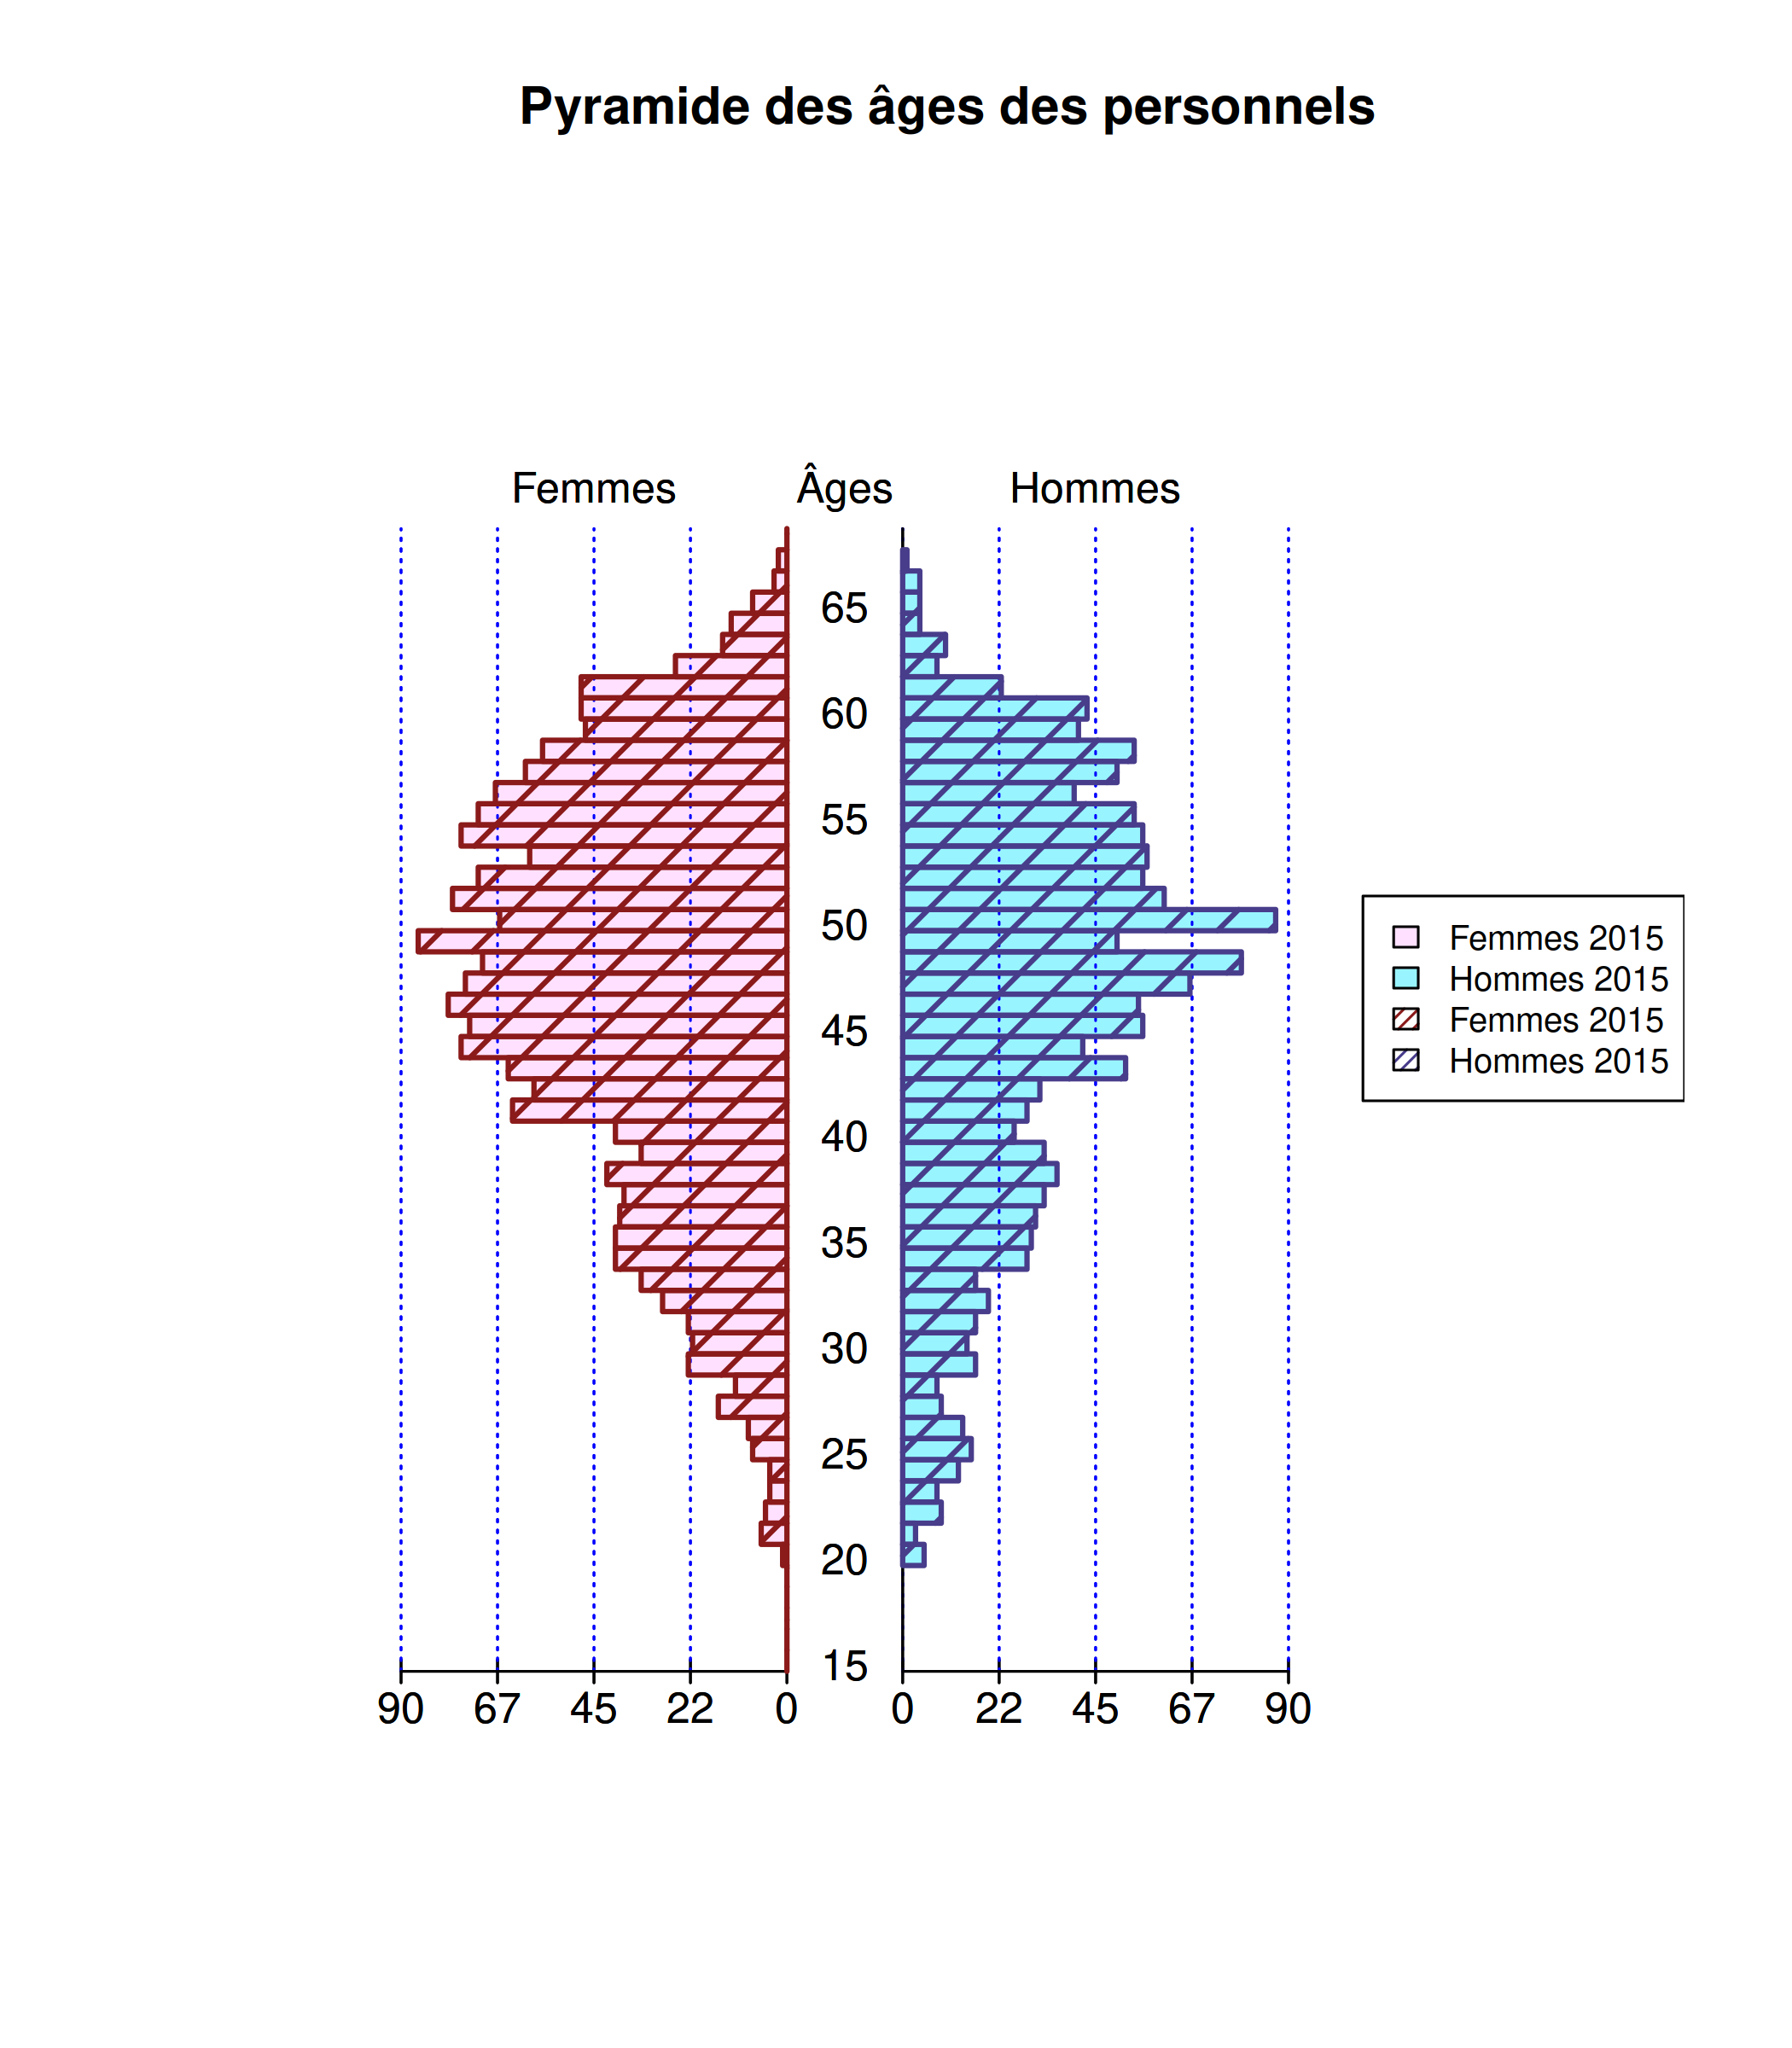
\includegraphics{altair_files/figure-latex/unnamed-chunk-11-1.png}
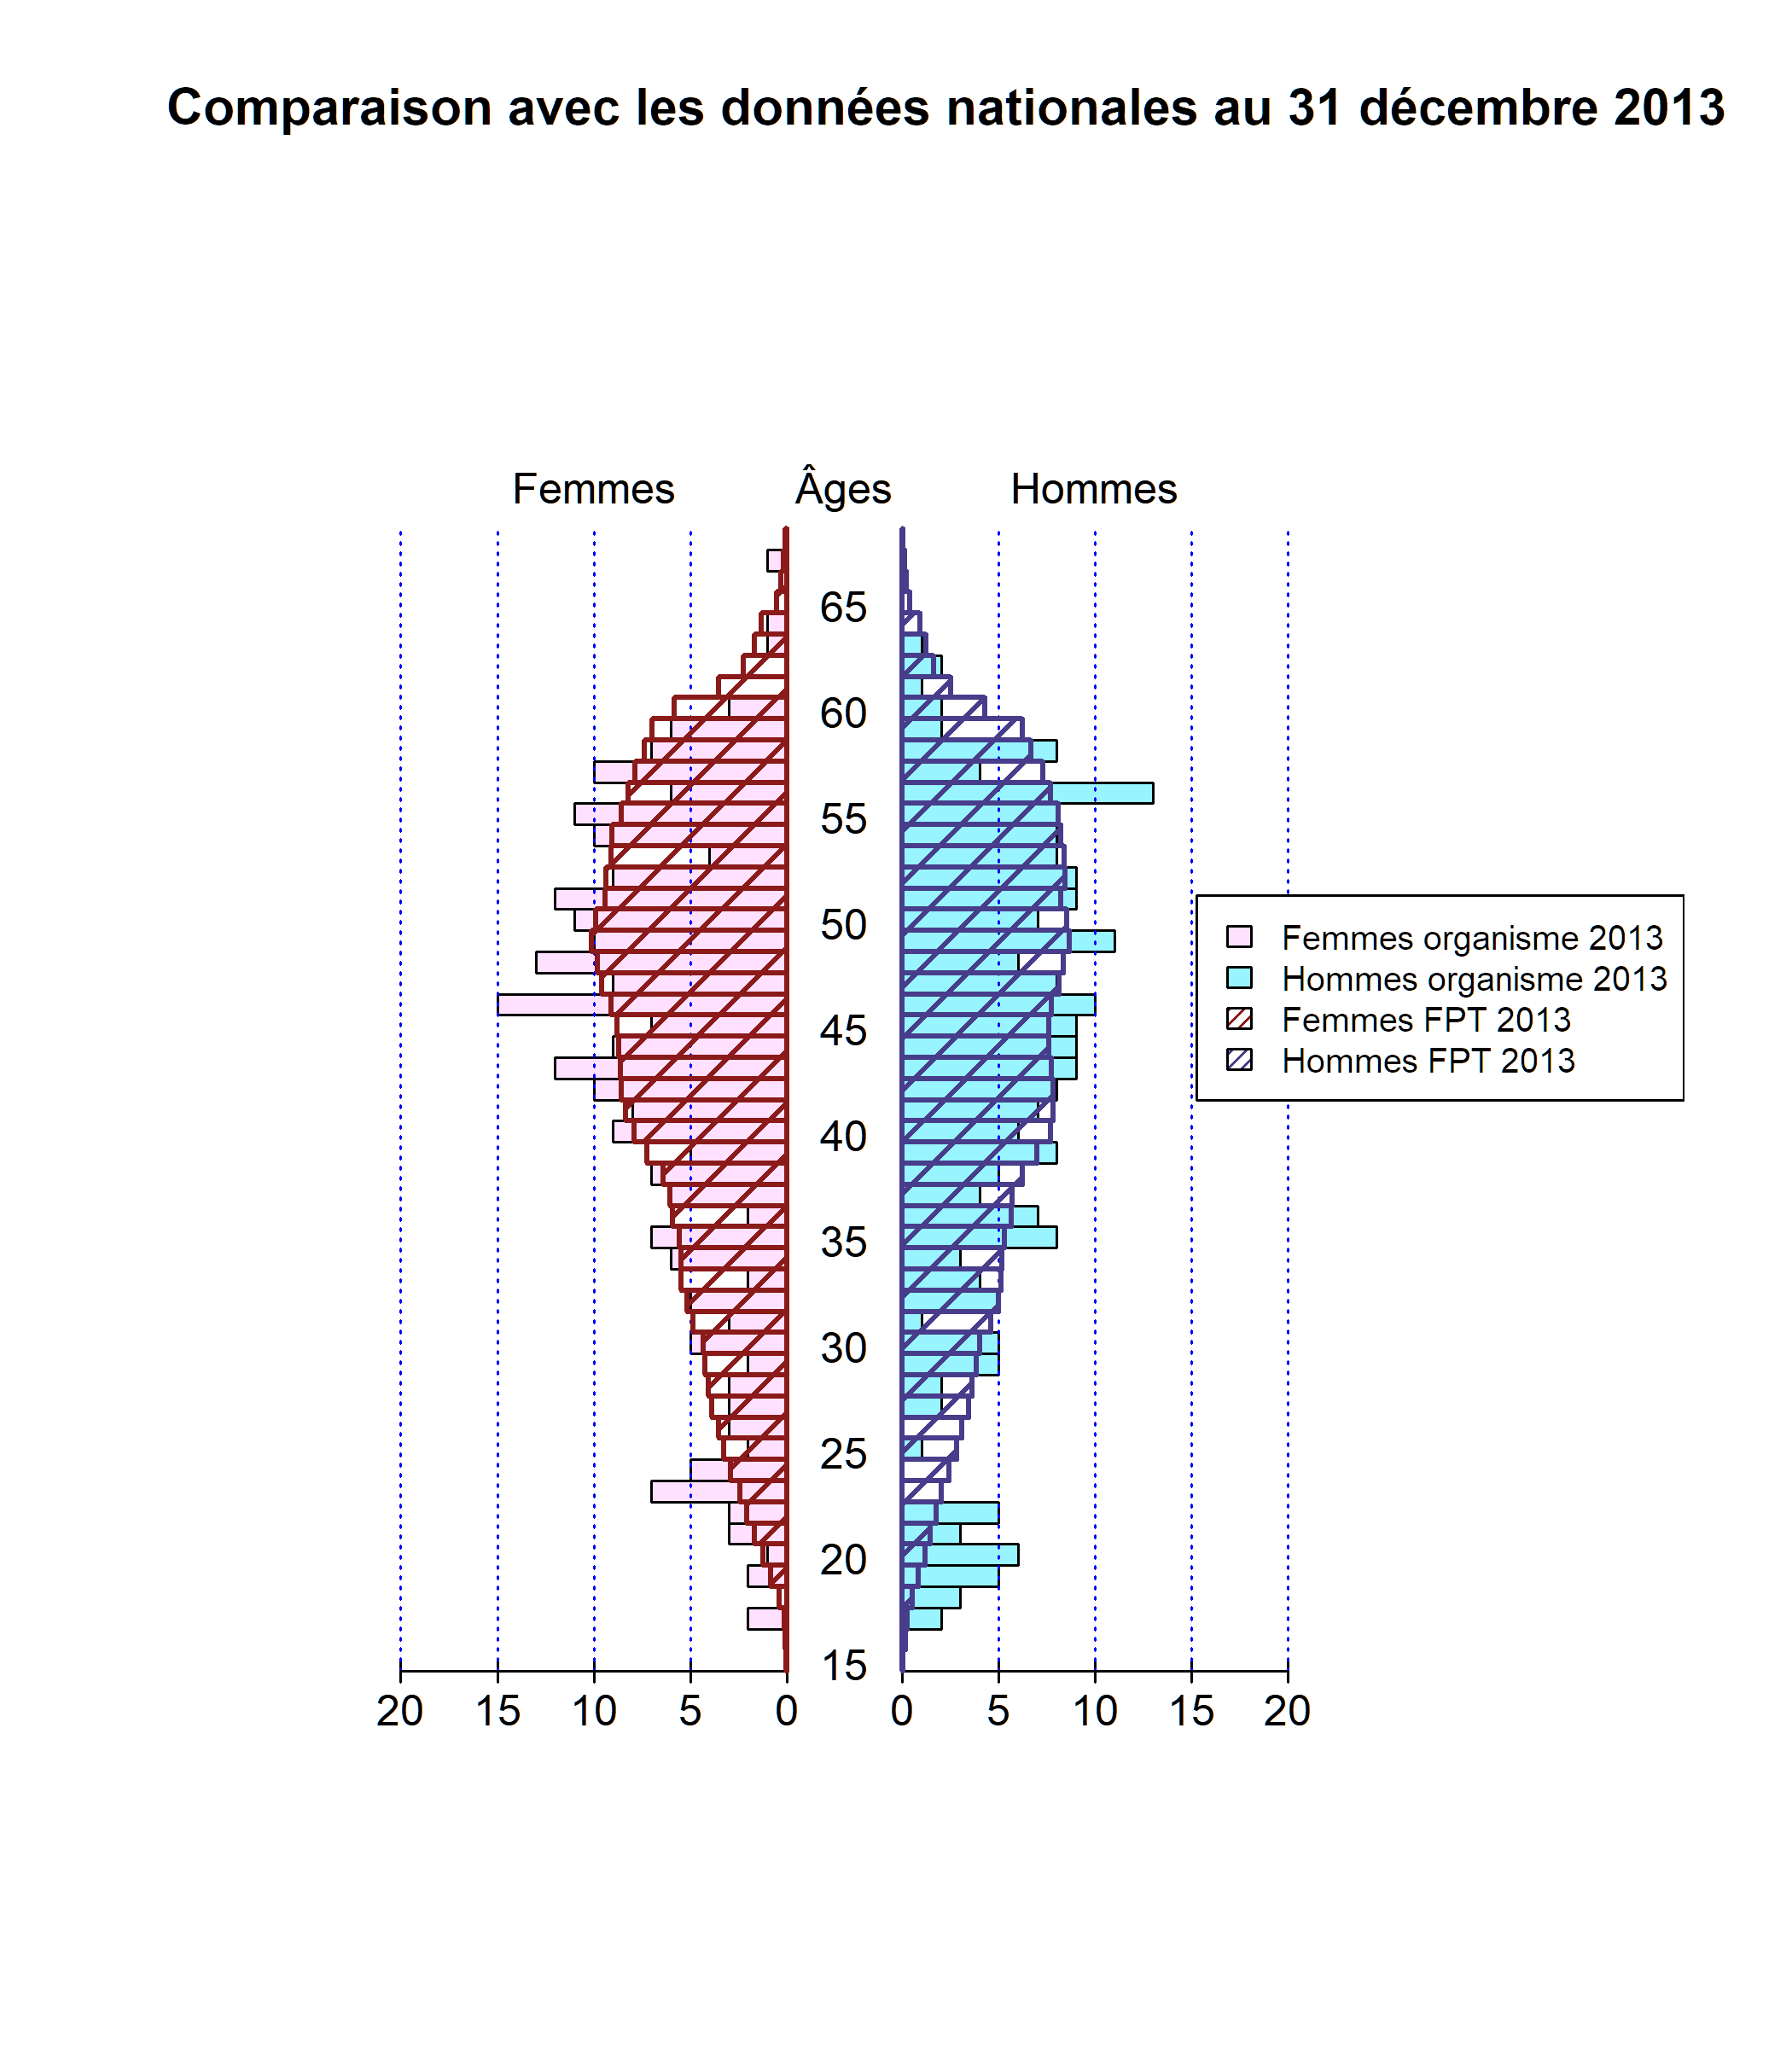
\includegraphics{altair_files/figure-latex/unnamed-chunk-11-2.png} Pour
obtenir les effectifs nationaux, multiplier les abscisses des hommes par
4 431 et les abscisses des femmes par 1 440\newpage
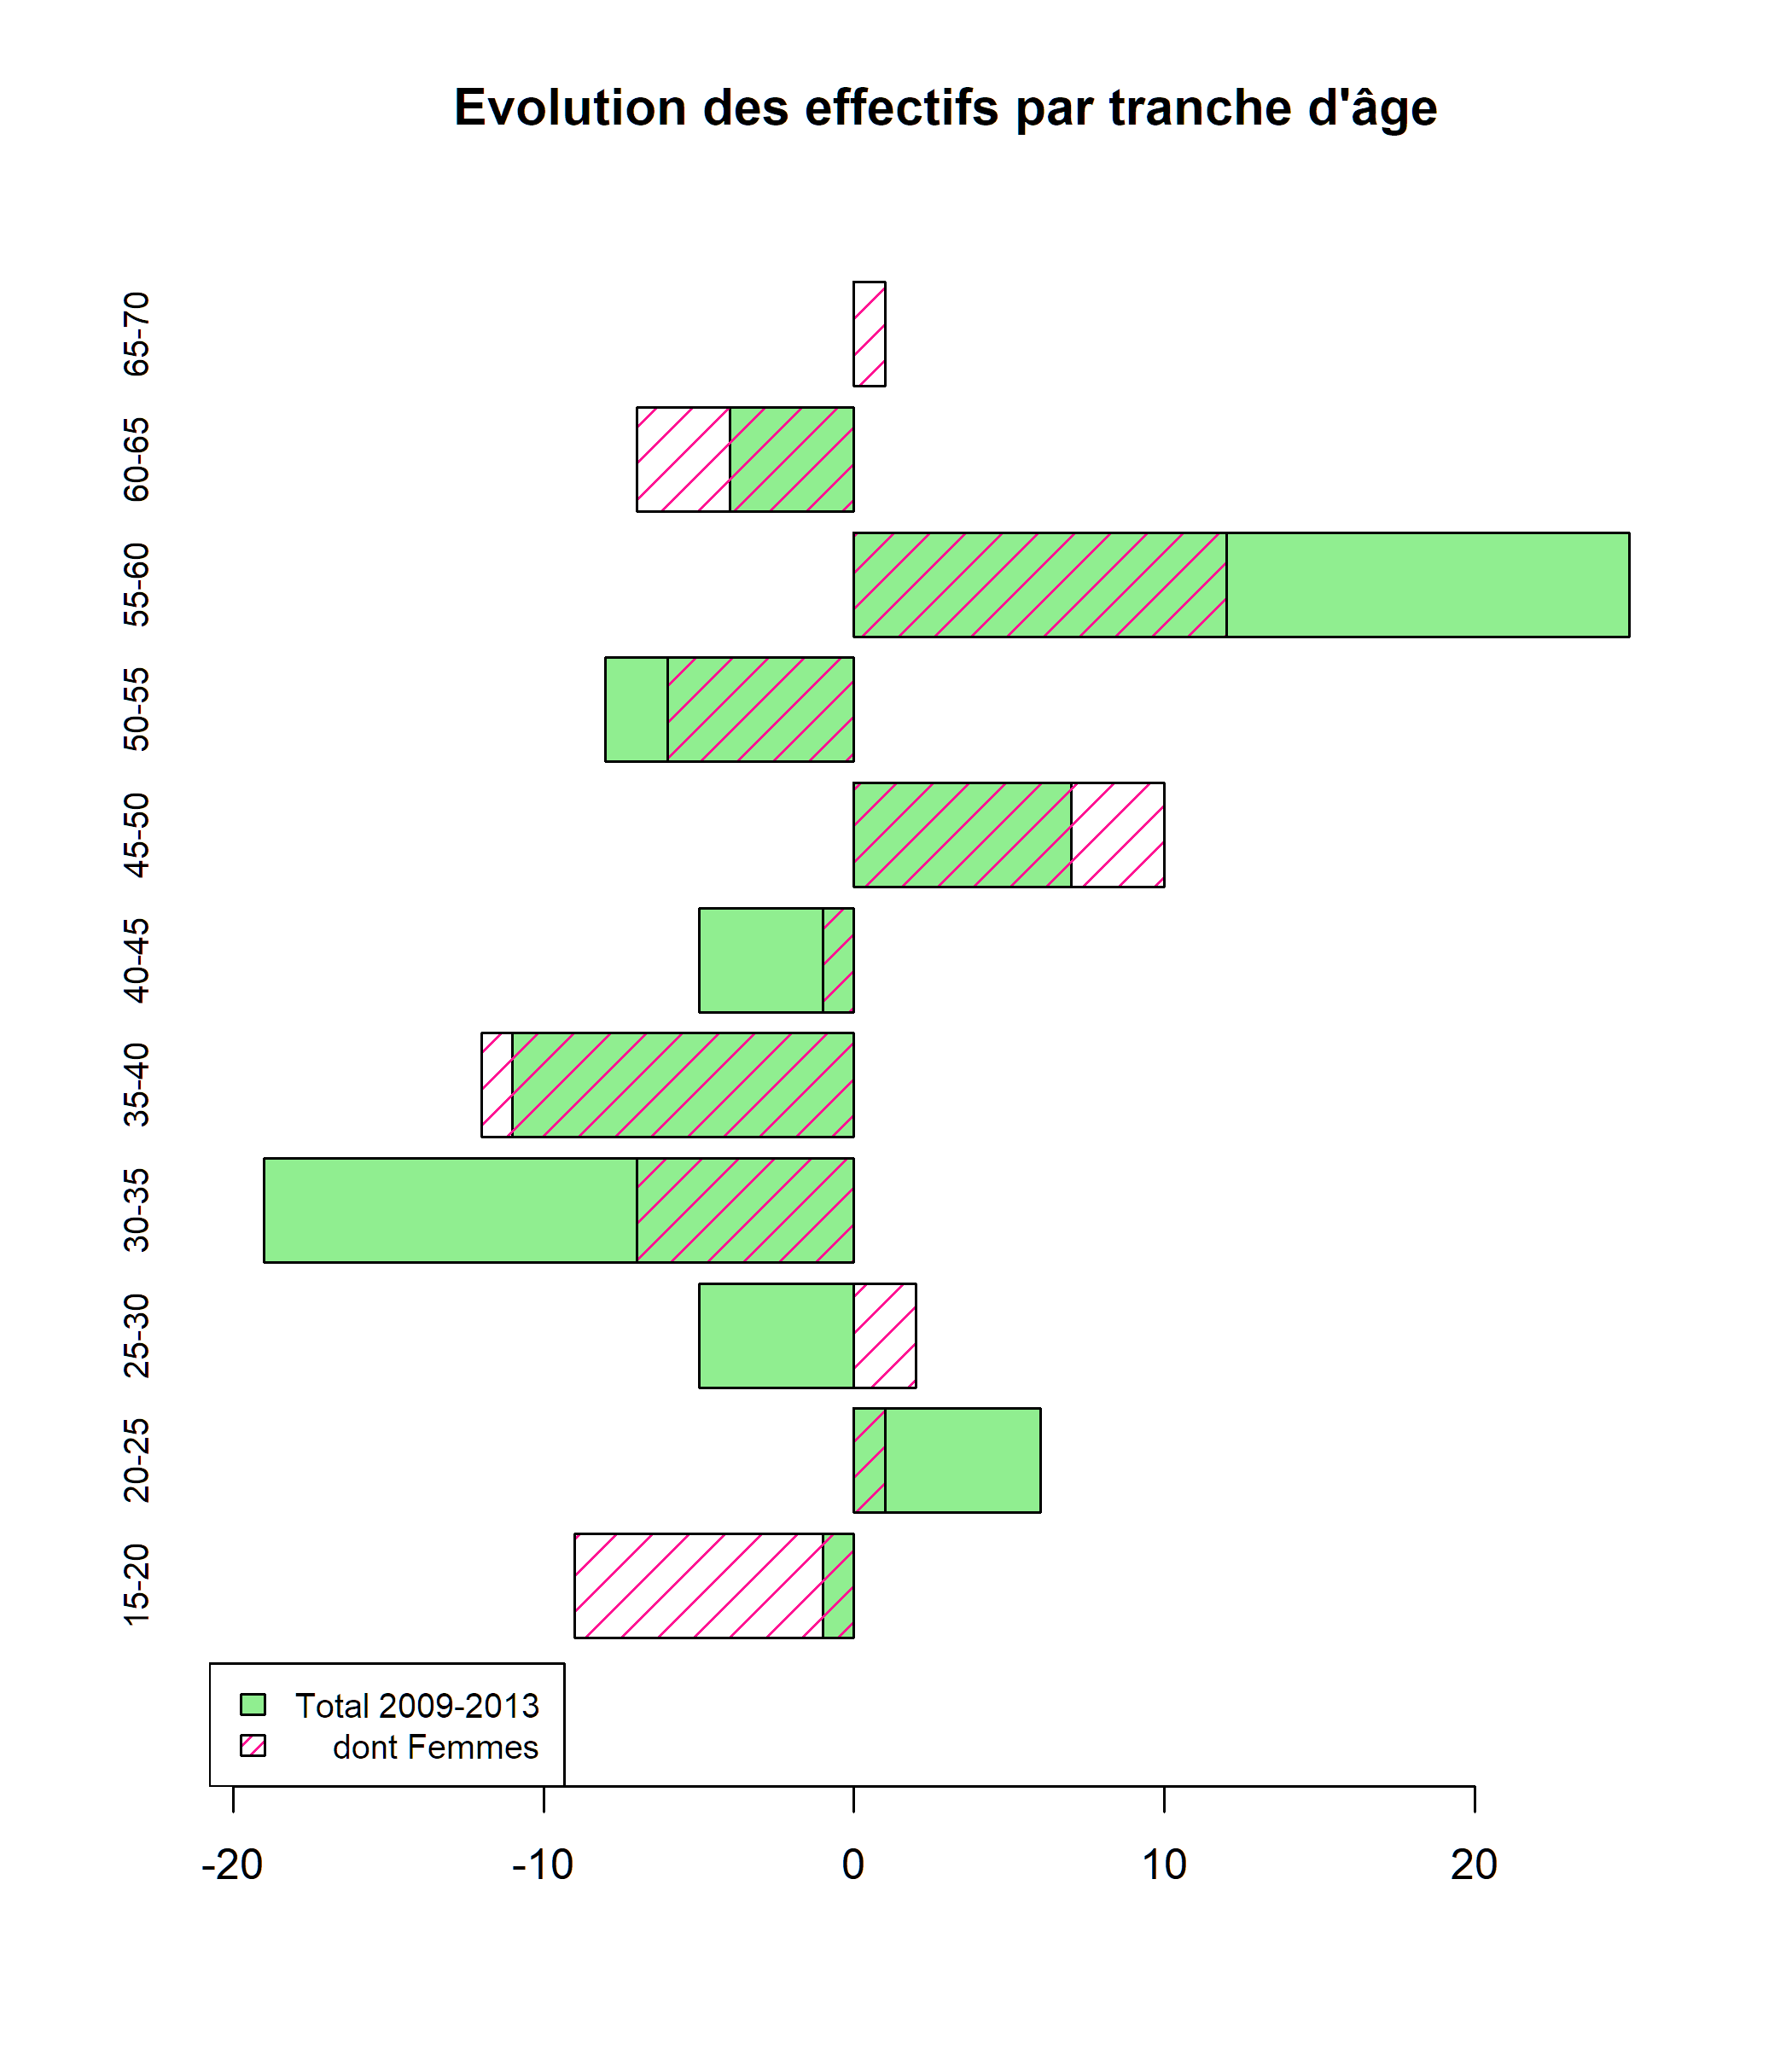
\includegraphics{altair_files/figure-latex/unnamed-chunk-11-3.png}

\href{../Docs/Notices/fiche_3.odt}{
\includegraphics{icones/Notice.png}}

\newpage

~\emph{Tableau 1.2.1}

\begin{longtable}[]{@{}ccccc@{}}
\toprule
\begin{minipage}[b]{0.12\columnwidth}\centering
Statistique\strut
\end{minipage} & \begin{minipage}[b]{0.29\columnwidth}\centering
Âge des personnels au 31/12/2011\strut
\end{minipage} & \begin{minipage}[b]{0.08\columnwidth}\centering
Effectif\strut
\end{minipage} & \begin{minipage}[b]{0.29\columnwidth}\centering
Âge des personnels au 31/12/2014\strut
\end{minipage} & \begin{minipage}[b]{0.08\columnwidth}\centering
Effectif\strut
\end{minipage}\tabularnewline
\midrule
\endhead
\begin{minipage}[t]{0.12\columnwidth}\centering
Minimum\strut
\end{minipage} & \begin{minipage}[t]{0.29\columnwidth}\centering
18,0\strut
\end{minipage} & \begin{minipage}[t]{0.08\columnwidth}\centering
\strut
\end{minipage} & \begin{minipage}[t]{0.29\columnwidth}\centering
18,0\strut
\end{minipage} & \begin{minipage}[t]{0.08\columnwidth}\centering
\strut
\end{minipage}\tabularnewline
\begin{minipage}[t]{0.12\columnwidth}\centering
1er quartile\strut
\end{minipage} & \begin{minipage}[t]{0.29\columnwidth}\centering
31,0\strut
\end{minipage} & \begin{minipage}[t]{0.08\columnwidth}\centering
\strut
\end{minipage} & \begin{minipage}[t]{0.29\columnwidth}\centering
32,0\strut
\end{minipage} & \begin{minipage}[t]{0.08\columnwidth}\centering
\strut
\end{minipage}\tabularnewline
\begin{minipage}[t]{0.12\columnwidth}\centering
Médiane\strut
\end{minipage} & \begin{minipage}[t]{0.29\columnwidth}\centering
41,0\strut
\end{minipage} & \begin{minipage}[t]{0.08\columnwidth}\centering
\strut
\end{minipage} & \begin{minipage}[t]{0.29\columnwidth}\centering
42,0\strut
\end{minipage} & \begin{minipage}[t]{0.08\columnwidth}\centering
\strut
\end{minipage}\tabularnewline
\begin{minipage}[t]{0.12\columnwidth}\centering
Moyenne\strut
\end{minipage} & \begin{minipage}[t]{0.29\columnwidth}\centering
40,1\strut
\end{minipage} & \begin{minipage}[t]{0.08\columnwidth}\centering
926\strut
\end{minipage} & \begin{minipage}[t]{0.29\columnwidth}\centering
40,9\strut
\end{minipage} & \begin{minipage}[t]{0.08\columnwidth}\centering
973\strut
\end{minipage}\tabularnewline
\begin{minipage}[t]{0.12\columnwidth}\centering
3ème quartile\strut
\end{minipage} & \begin{minipage}[t]{0.29\columnwidth}\centering
49,0\strut
\end{minipage} & \begin{minipage}[t]{0.08\columnwidth}\centering
\strut
\end{minipage} & \begin{minipage}[t]{0.29\columnwidth}\centering
50,0\strut
\end{minipage} & \begin{minipage}[t]{0.08\columnwidth}\centering
\strut
\end{minipage}\tabularnewline
\begin{minipage}[t]{0.12\columnwidth}\centering
Maximum\strut
\end{minipage} & \begin{minipage}[t]{0.29\columnwidth}\centering
74,0\strut
\end{minipage} & \begin{minipage}[t]{0.08\columnwidth}\centering
\strut
\end{minipage} & \begin{minipage}[t]{0.29\columnwidth}\centering
72,0\strut
\end{minipage} & \begin{minipage}[t]{0.08\columnwidth}\centering
\strut
\end{minipage}\tabularnewline
\bottomrule
\end{longtable}

\href{../Docs/Notices/fiche_1.odt}{
\includegraphics{icones/Notice.png}}

\href{../Bases/Effectifs/Pyramide-des-ages-des-personnels_2011.csv}{Lien
vers la base des âges - début de periode}

\href{../Bases/Effectifs/Pyramide-des-ages-des-personnels_2014.csv}{Lien
vers la base des âges - fin de periode}

\hypertarget{pyramide-des-ages-des-fonctionnaires}{%
\subsection{1.3 Pyramide des âges des fonctionnaires
~}\label{pyramide-des-ages-des-fonctionnaires}}

\href{../Docs/Notices/fiche_2.odt}{
\includegraphics{icones/Notice.png}}

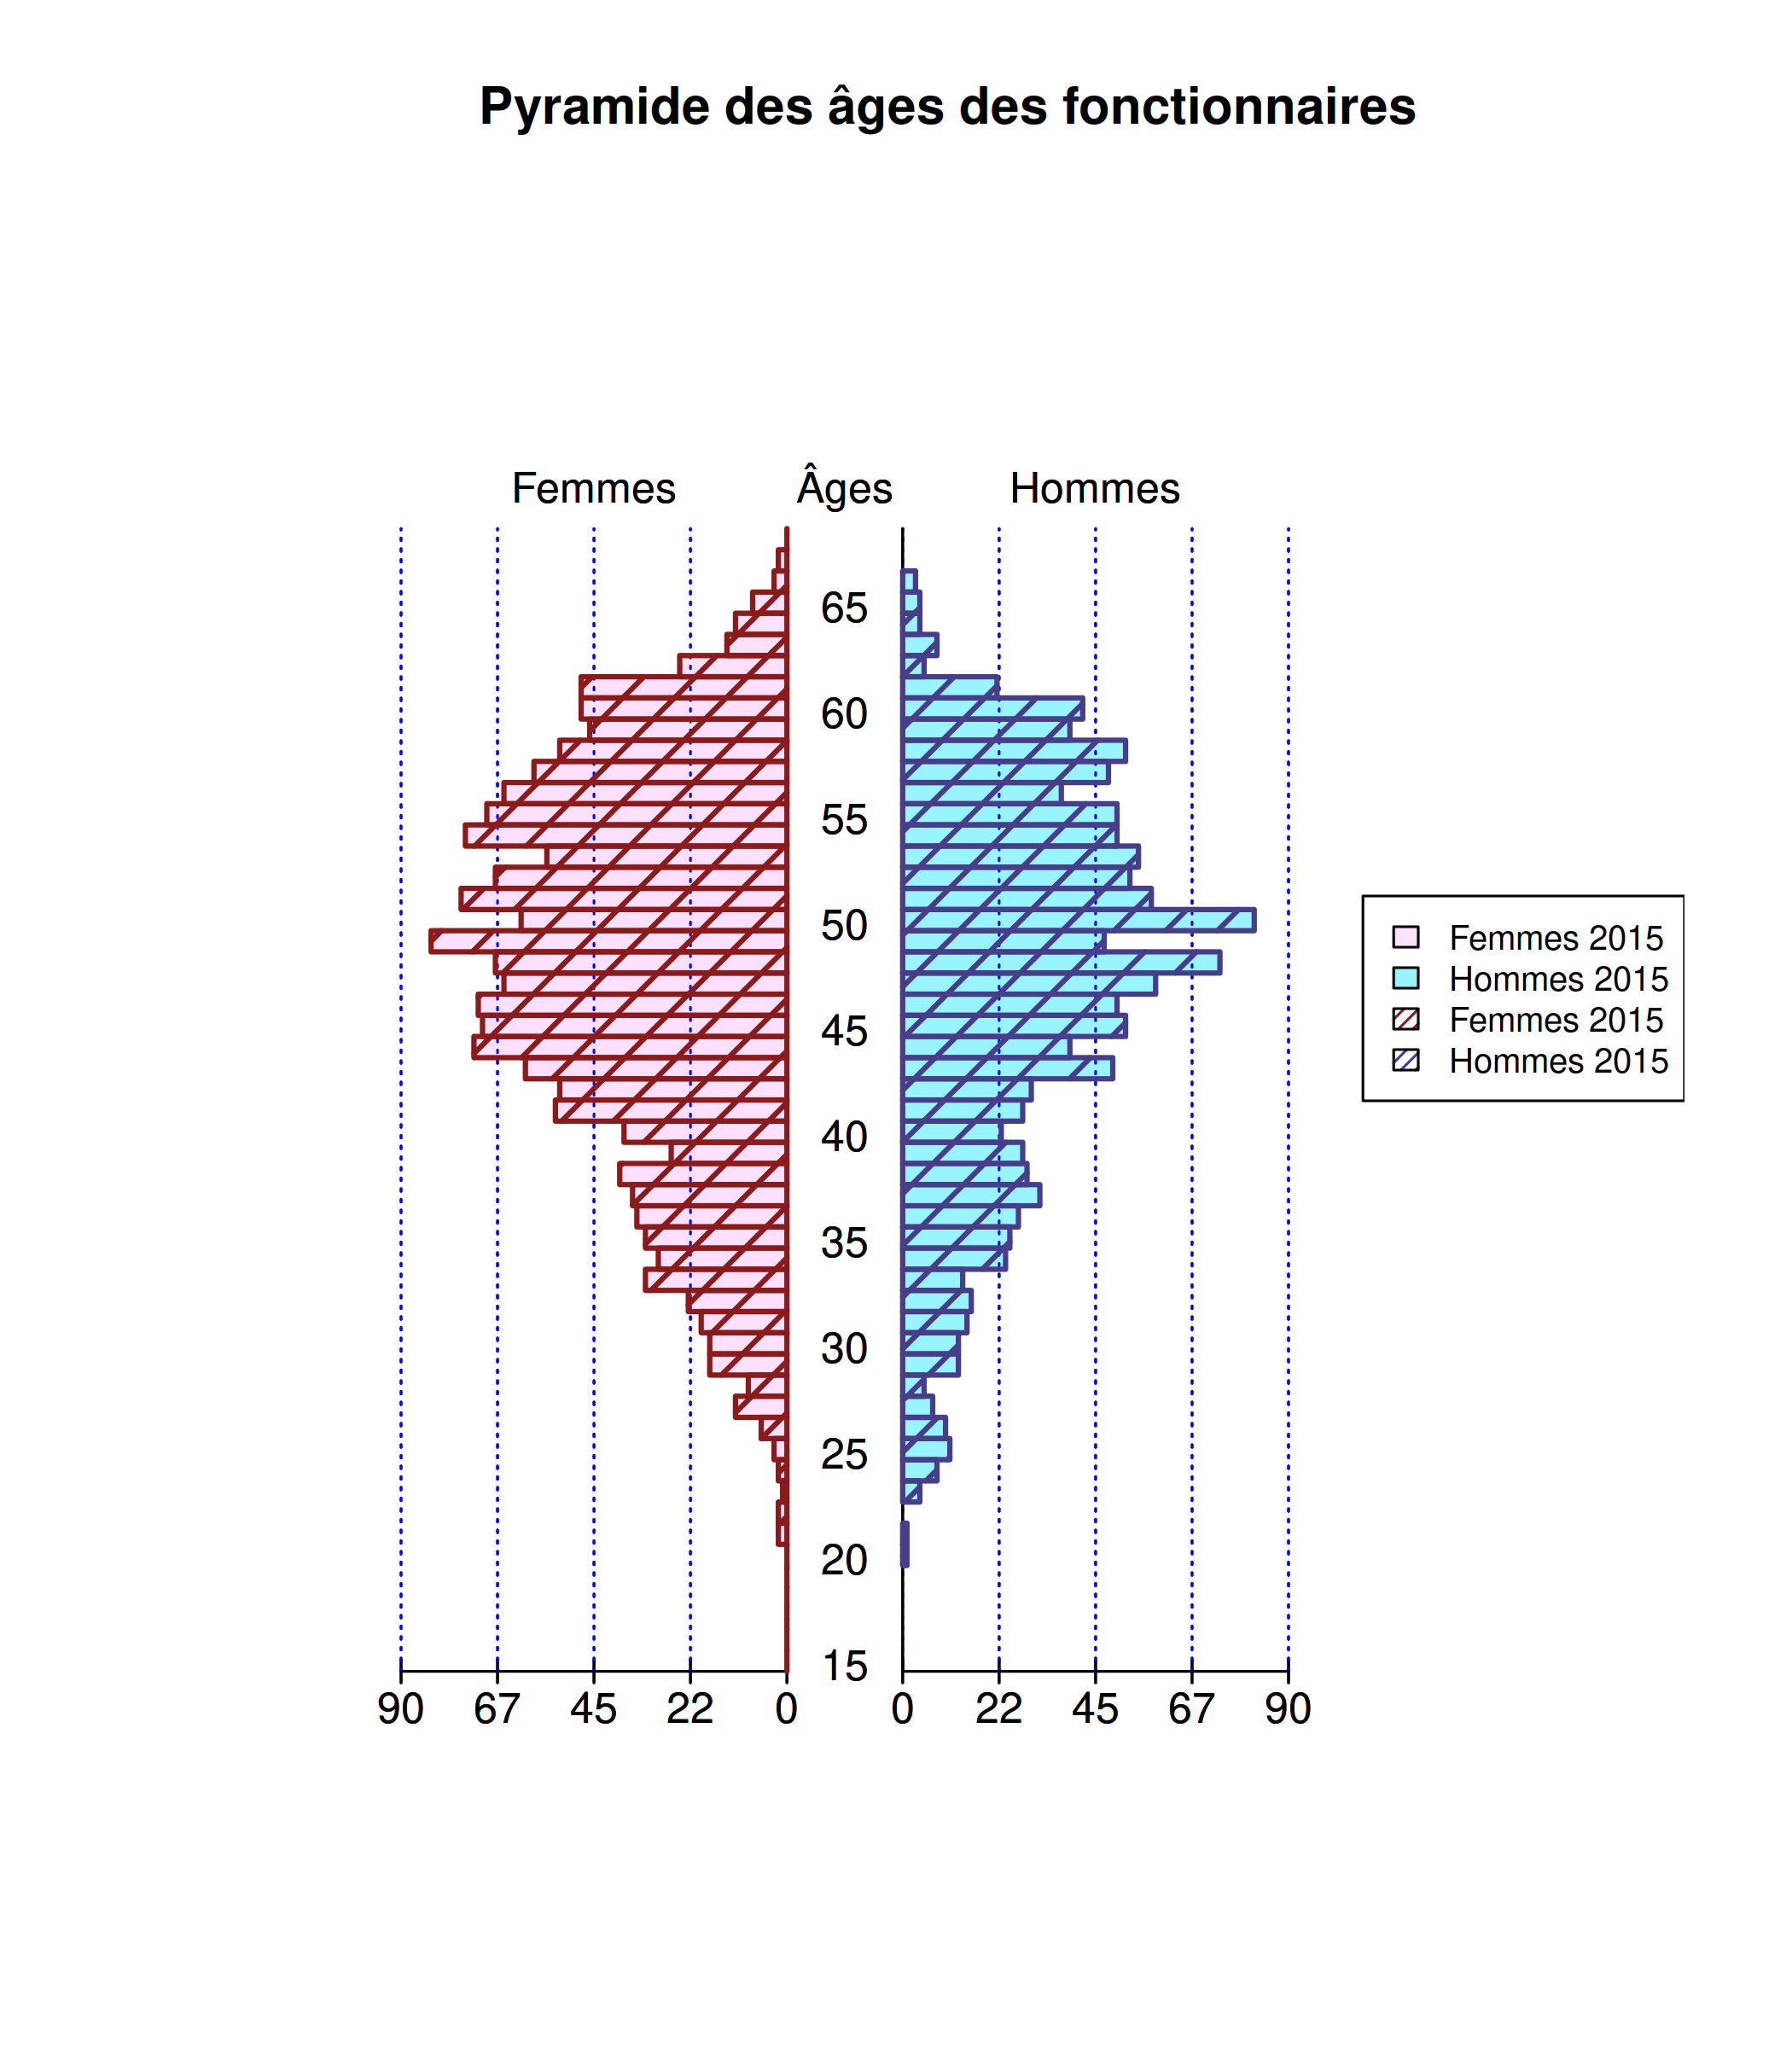
\includegraphics{altair_files/figure-latex/unnamed-chunk-17-1.png}
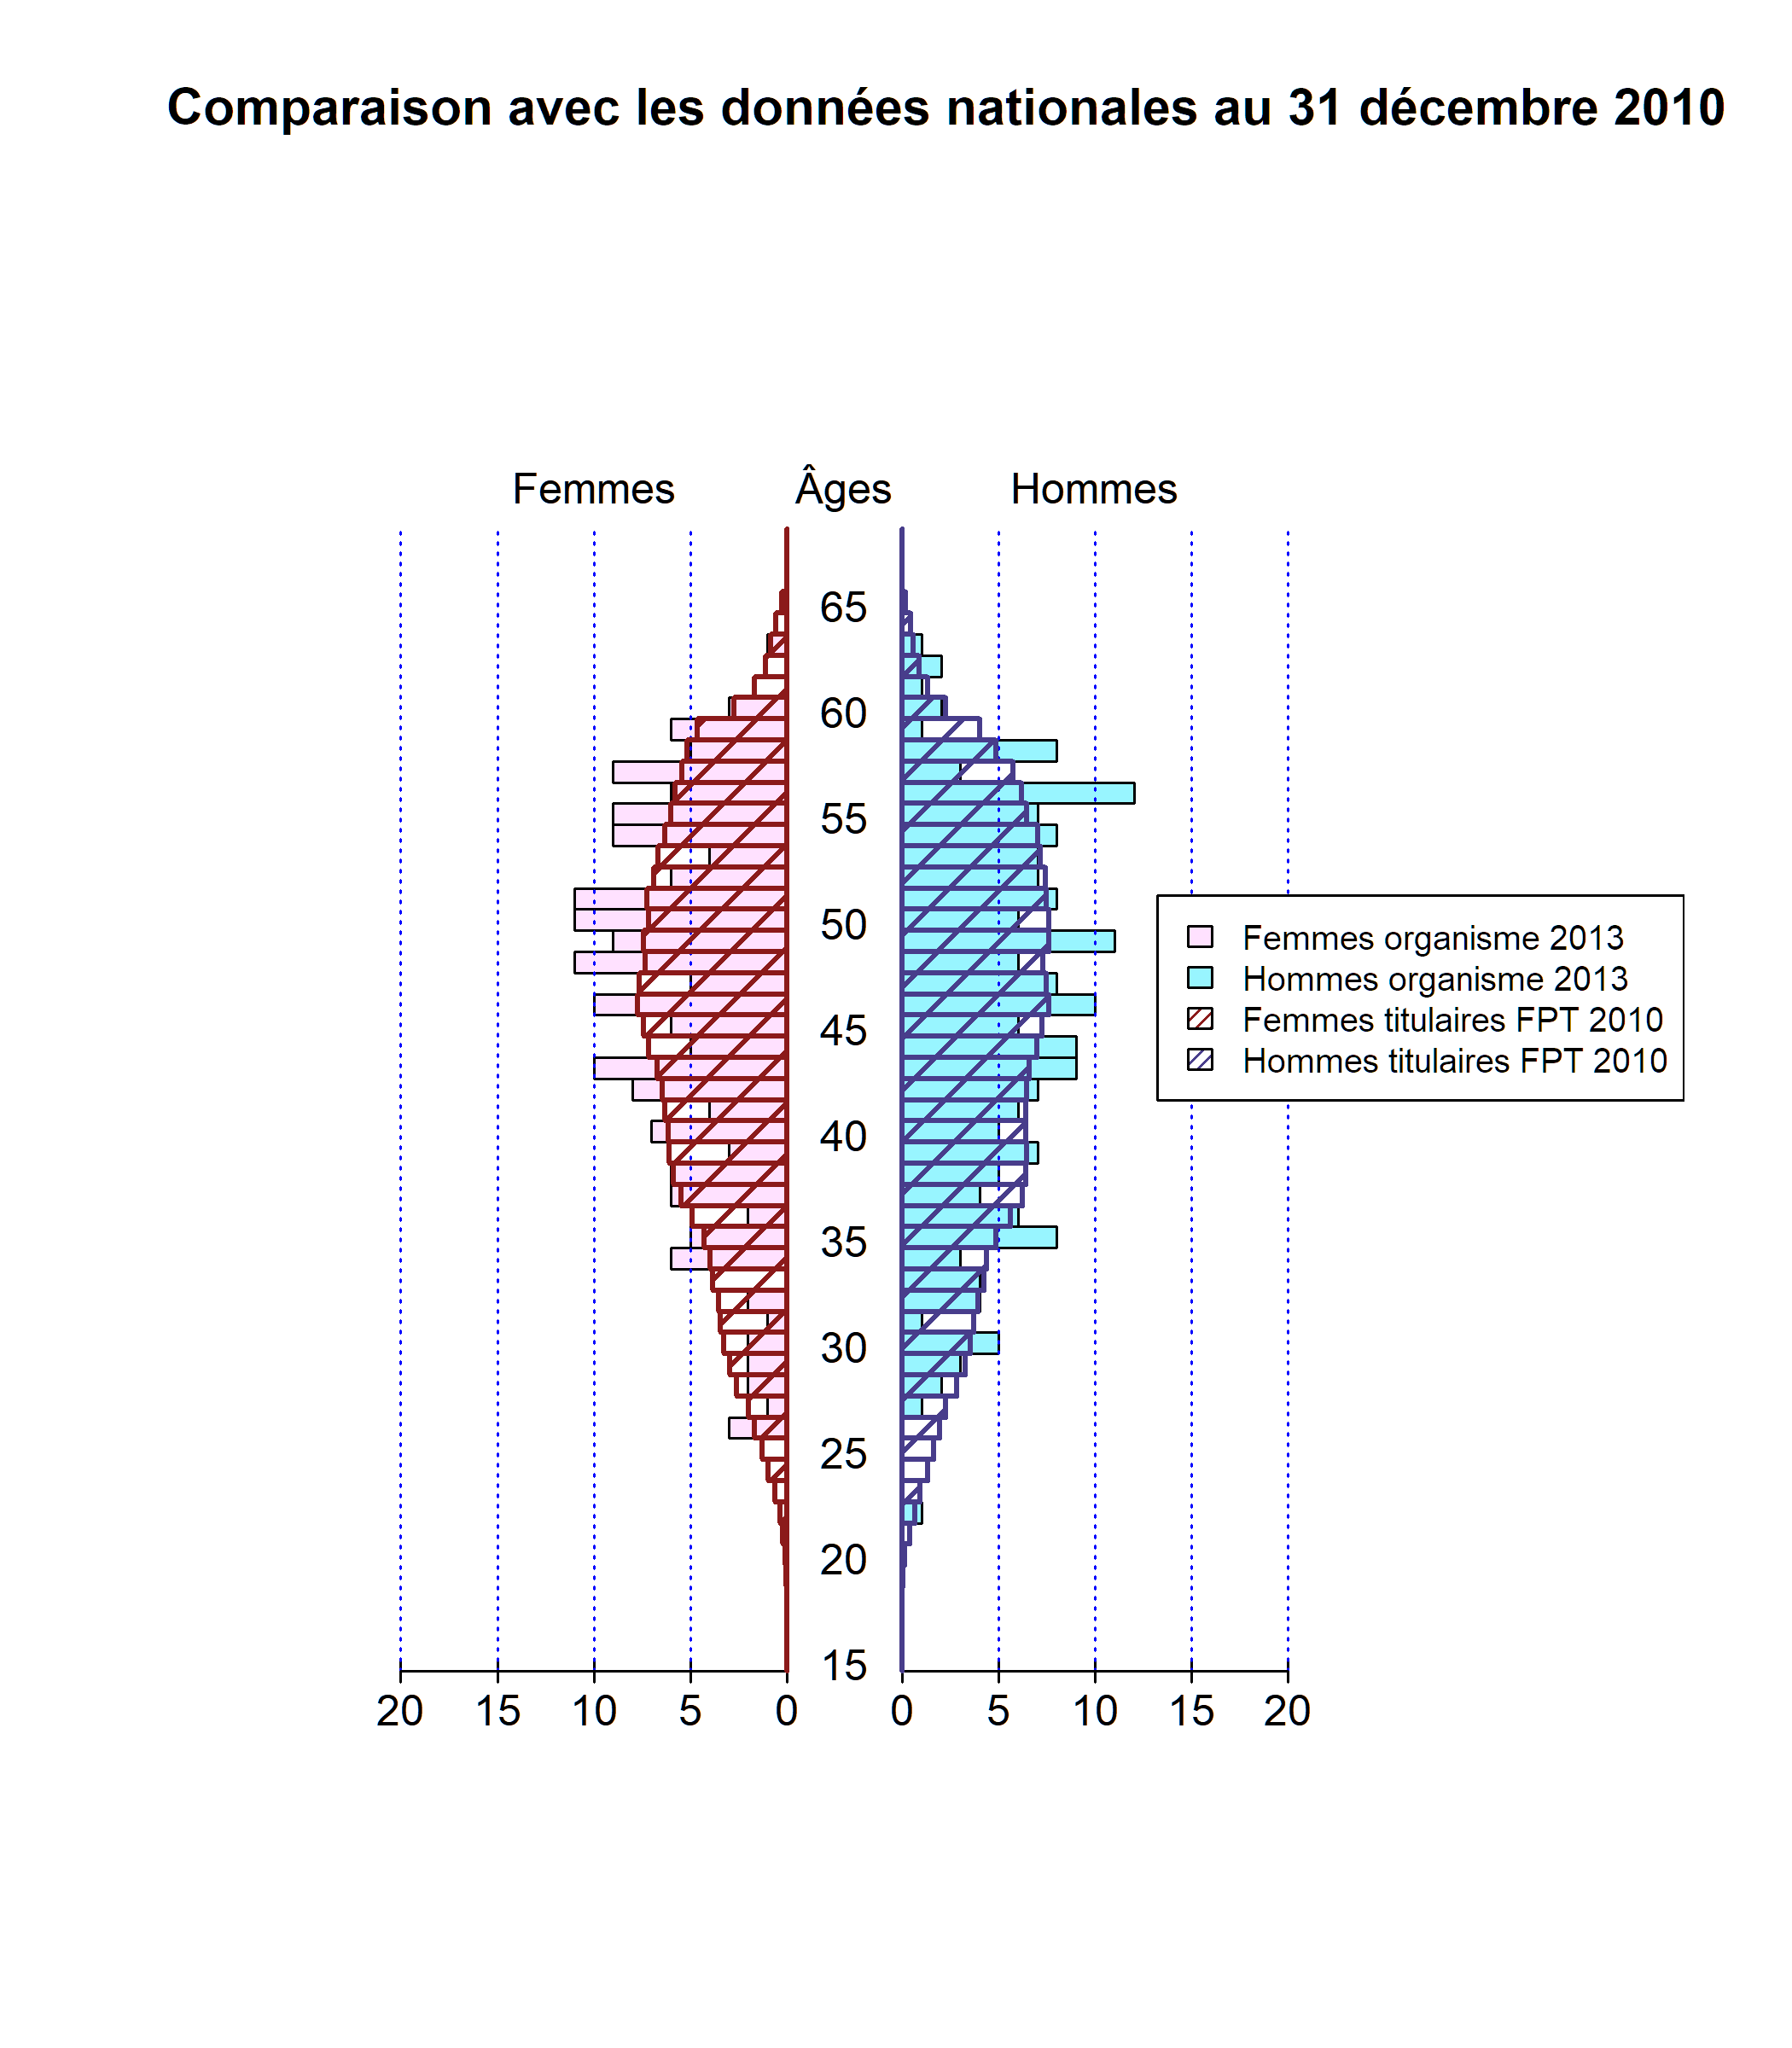
\includegraphics{altair_files/figure-latex/unnamed-chunk-17-2.png} Pour
obtenir les effectifs nationaux, multiplier les abscisses des hommes par
6 051 et les abscisses des femmes par 443\newpage
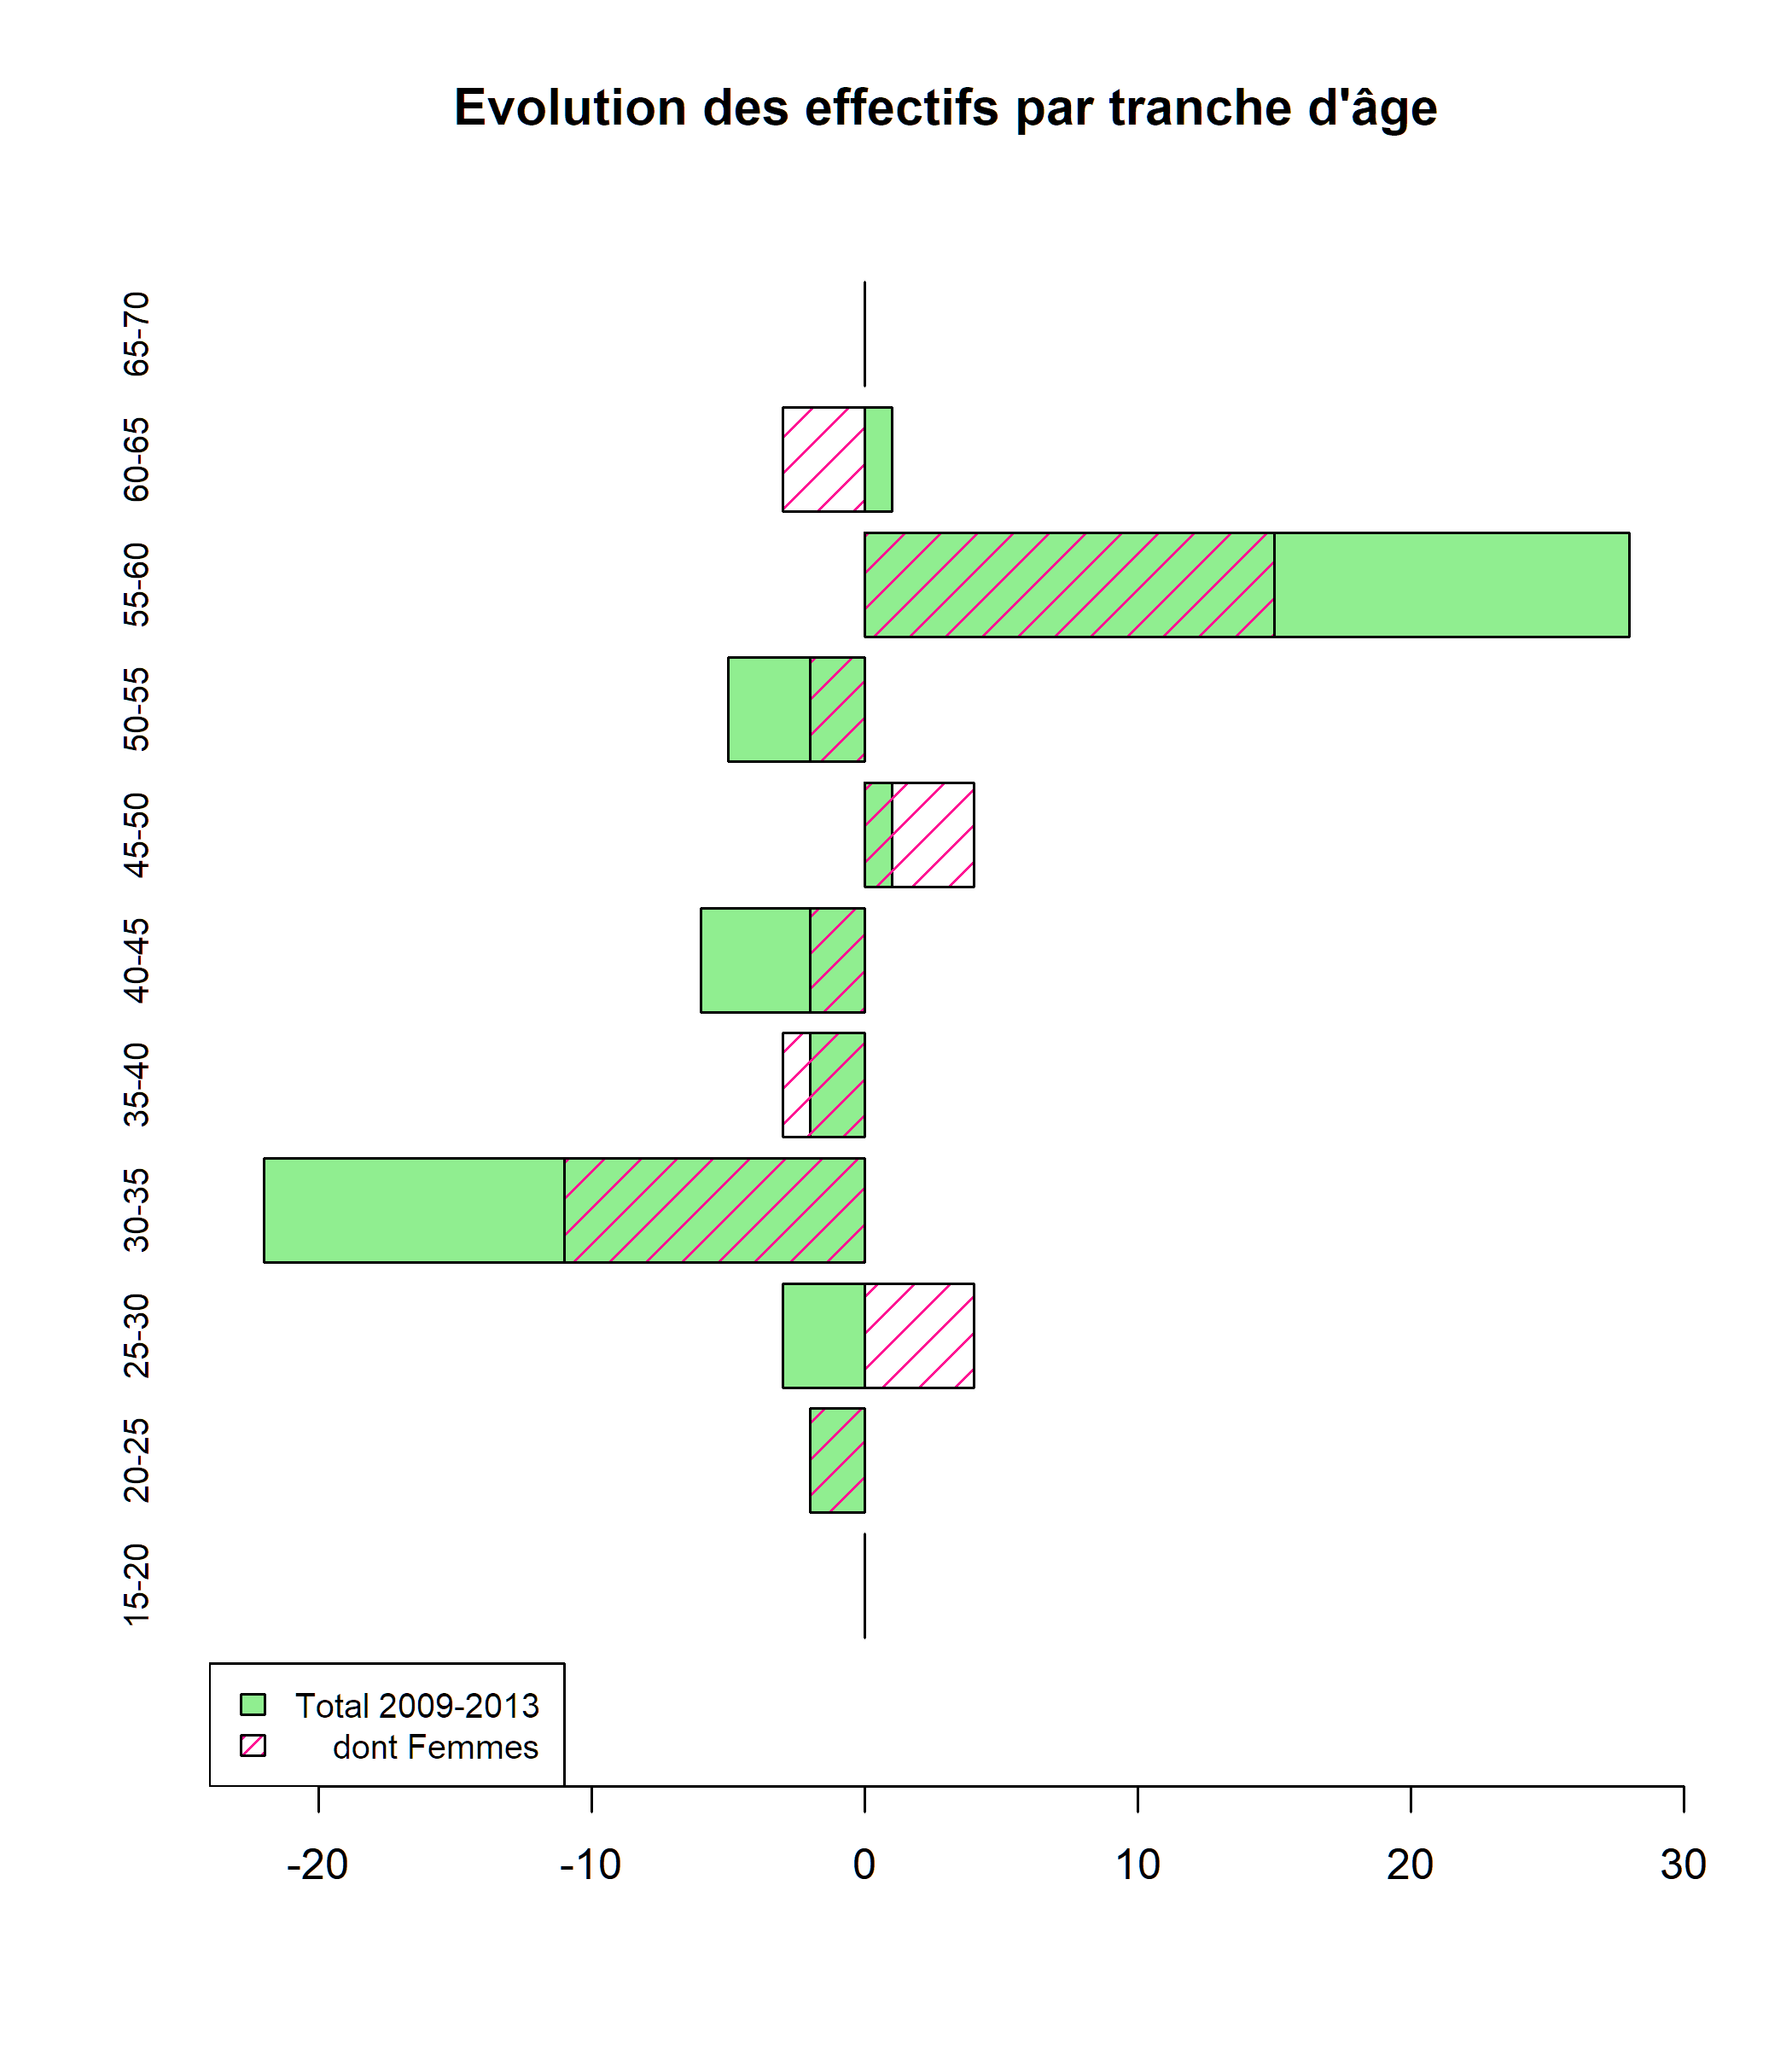
\includegraphics{altair_files/figure-latex/unnamed-chunk-17-3.png}

\href{../Docs/Notices/fiche_3.odt}{
\includegraphics{icones/Notice.png}}

\newpage

~\emph{Tableau 1.3.1}

\begin{longtable}[]{@{}ccccc@{}}
\toprule
\begin{minipage}[b]{0.12\columnwidth}\centering
Statistique\strut
\end{minipage} & \begin{minipage}[b]{0.29\columnwidth}\centering
Âge des personnels au 31/12/2011\strut
\end{minipage} & \begin{minipage}[b]{0.08\columnwidth}\centering
Effectif\strut
\end{minipage} & \begin{minipage}[b]{0.29\columnwidth}\centering
Âge des personnels au 31/12/2014\strut
\end{minipage} & \begin{minipage}[b]{0.08\columnwidth}\centering
Effectif\strut
\end{minipage}\tabularnewline
\midrule
\endhead
\begin{minipage}[t]{0.12\columnwidth}\centering
Minimum\strut
\end{minipage} & \begin{minipage}[t]{0.29\columnwidth}\centering
25,0\strut
\end{minipage} & \begin{minipage}[t]{0.08\columnwidth}\centering
\strut
\end{minipage} & \begin{minipage}[t]{0.29\columnwidth}\centering
25,0\strut
\end{minipage} & \begin{minipage}[t]{0.08\columnwidth}\centering
\strut
\end{minipage}\tabularnewline
\begin{minipage}[t]{0.12\columnwidth}\centering
1er quartile\strut
\end{minipage} & \begin{minipage}[t]{0.29\columnwidth}\centering
36,0\strut
\end{minipage} & \begin{minipage}[t]{0.08\columnwidth}\centering
\strut
\end{minipage} & \begin{minipage}[t]{0.29\columnwidth}\centering
37,0\strut
\end{minipage} & \begin{minipage}[t]{0.08\columnwidth}\centering
\strut
\end{minipage}\tabularnewline
\begin{minipage}[t]{0.12\columnwidth}\centering
Médiane\strut
\end{minipage} & \begin{minipage}[t]{0.29\columnwidth}\centering
43,0\strut
\end{minipage} & \begin{minipage}[t]{0.08\columnwidth}\centering
\strut
\end{minipage} & \begin{minipage}[t]{0.29\columnwidth}\centering
44,0\strut
\end{minipage} & \begin{minipage}[t]{0.08\columnwidth}\centering
\strut
\end{minipage}\tabularnewline
\begin{minipage}[t]{0.12\columnwidth}\centering
Moyenne\strut
\end{minipage} & \begin{minipage}[t]{0.29\columnwidth}\centering
43,1\strut
\end{minipage} & \begin{minipage}[t]{0.08\columnwidth}\centering
612\strut
\end{minipage} & \begin{minipage}[t]{0.29\columnwidth}\centering
44,1\strut
\end{minipage} & \begin{minipage}[t]{0.08\columnwidth}\centering
615\strut
\end{minipage}\tabularnewline
\begin{minipage}[t]{0.12\columnwidth}\centering
3ème quartile\strut
\end{minipage} & \begin{minipage}[t]{0.29\columnwidth}\centering
50,0\strut
\end{minipage} & \begin{minipage}[t]{0.08\columnwidth}\centering
\strut
\end{minipage} & \begin{minipage}[t]{0.29\columnwidth}\centering
51,0\strut
\end{minipage} & \begin{minipage}[t]{0.08\columnwidth}\centering
\strut
\end{minipage}\tabularnewline
\begin{minipage}[t]{0.12\columnwidth}\centering
Maximum\strut
\end{minipage} & \begin{minipage}[t]{0.29\columnwidth}\centering
60,0\strut
\end{minipage} & \begin{minipage}[t]{0.08\columnwidth}\centering
\strut
\end{minipage} & \begin{minipage}[t]{0.29\columnwidth}\centering
62,0\strut
\end{minipage} & \begin{minipage}[t]{0.08\columnwidth}\centering
\strut
\end{minipage}\tabularnewline
\bottomrule
\end{longtable}

\href{../Bases/Effectifs/Pyramide-des-ages-des-fonctionnaires_2011.csv}{Lien
vers la base des âges - début de periode}

\href{../Bases/Effectifs/Pyramide-des-ages-des-fonctionnaires_2014.csv}{Lien
vers la base des âges - fin de periode}

\href{../Docs/Notices/fiche_1.odt}{
\includegraphics{icones/Notice.png}}

\hypertarget{pyramide-des-ages-personnels-non-titulaires}{%
\subsection{1.4 Pyramide des âges, personnels non titulaires
~}\label{pyramide-des-ages-personnels-non-titulaires}}

\href{../Docs/Notices/fiche_2.odt}{
\includegraphics{icones/Notice.png}}

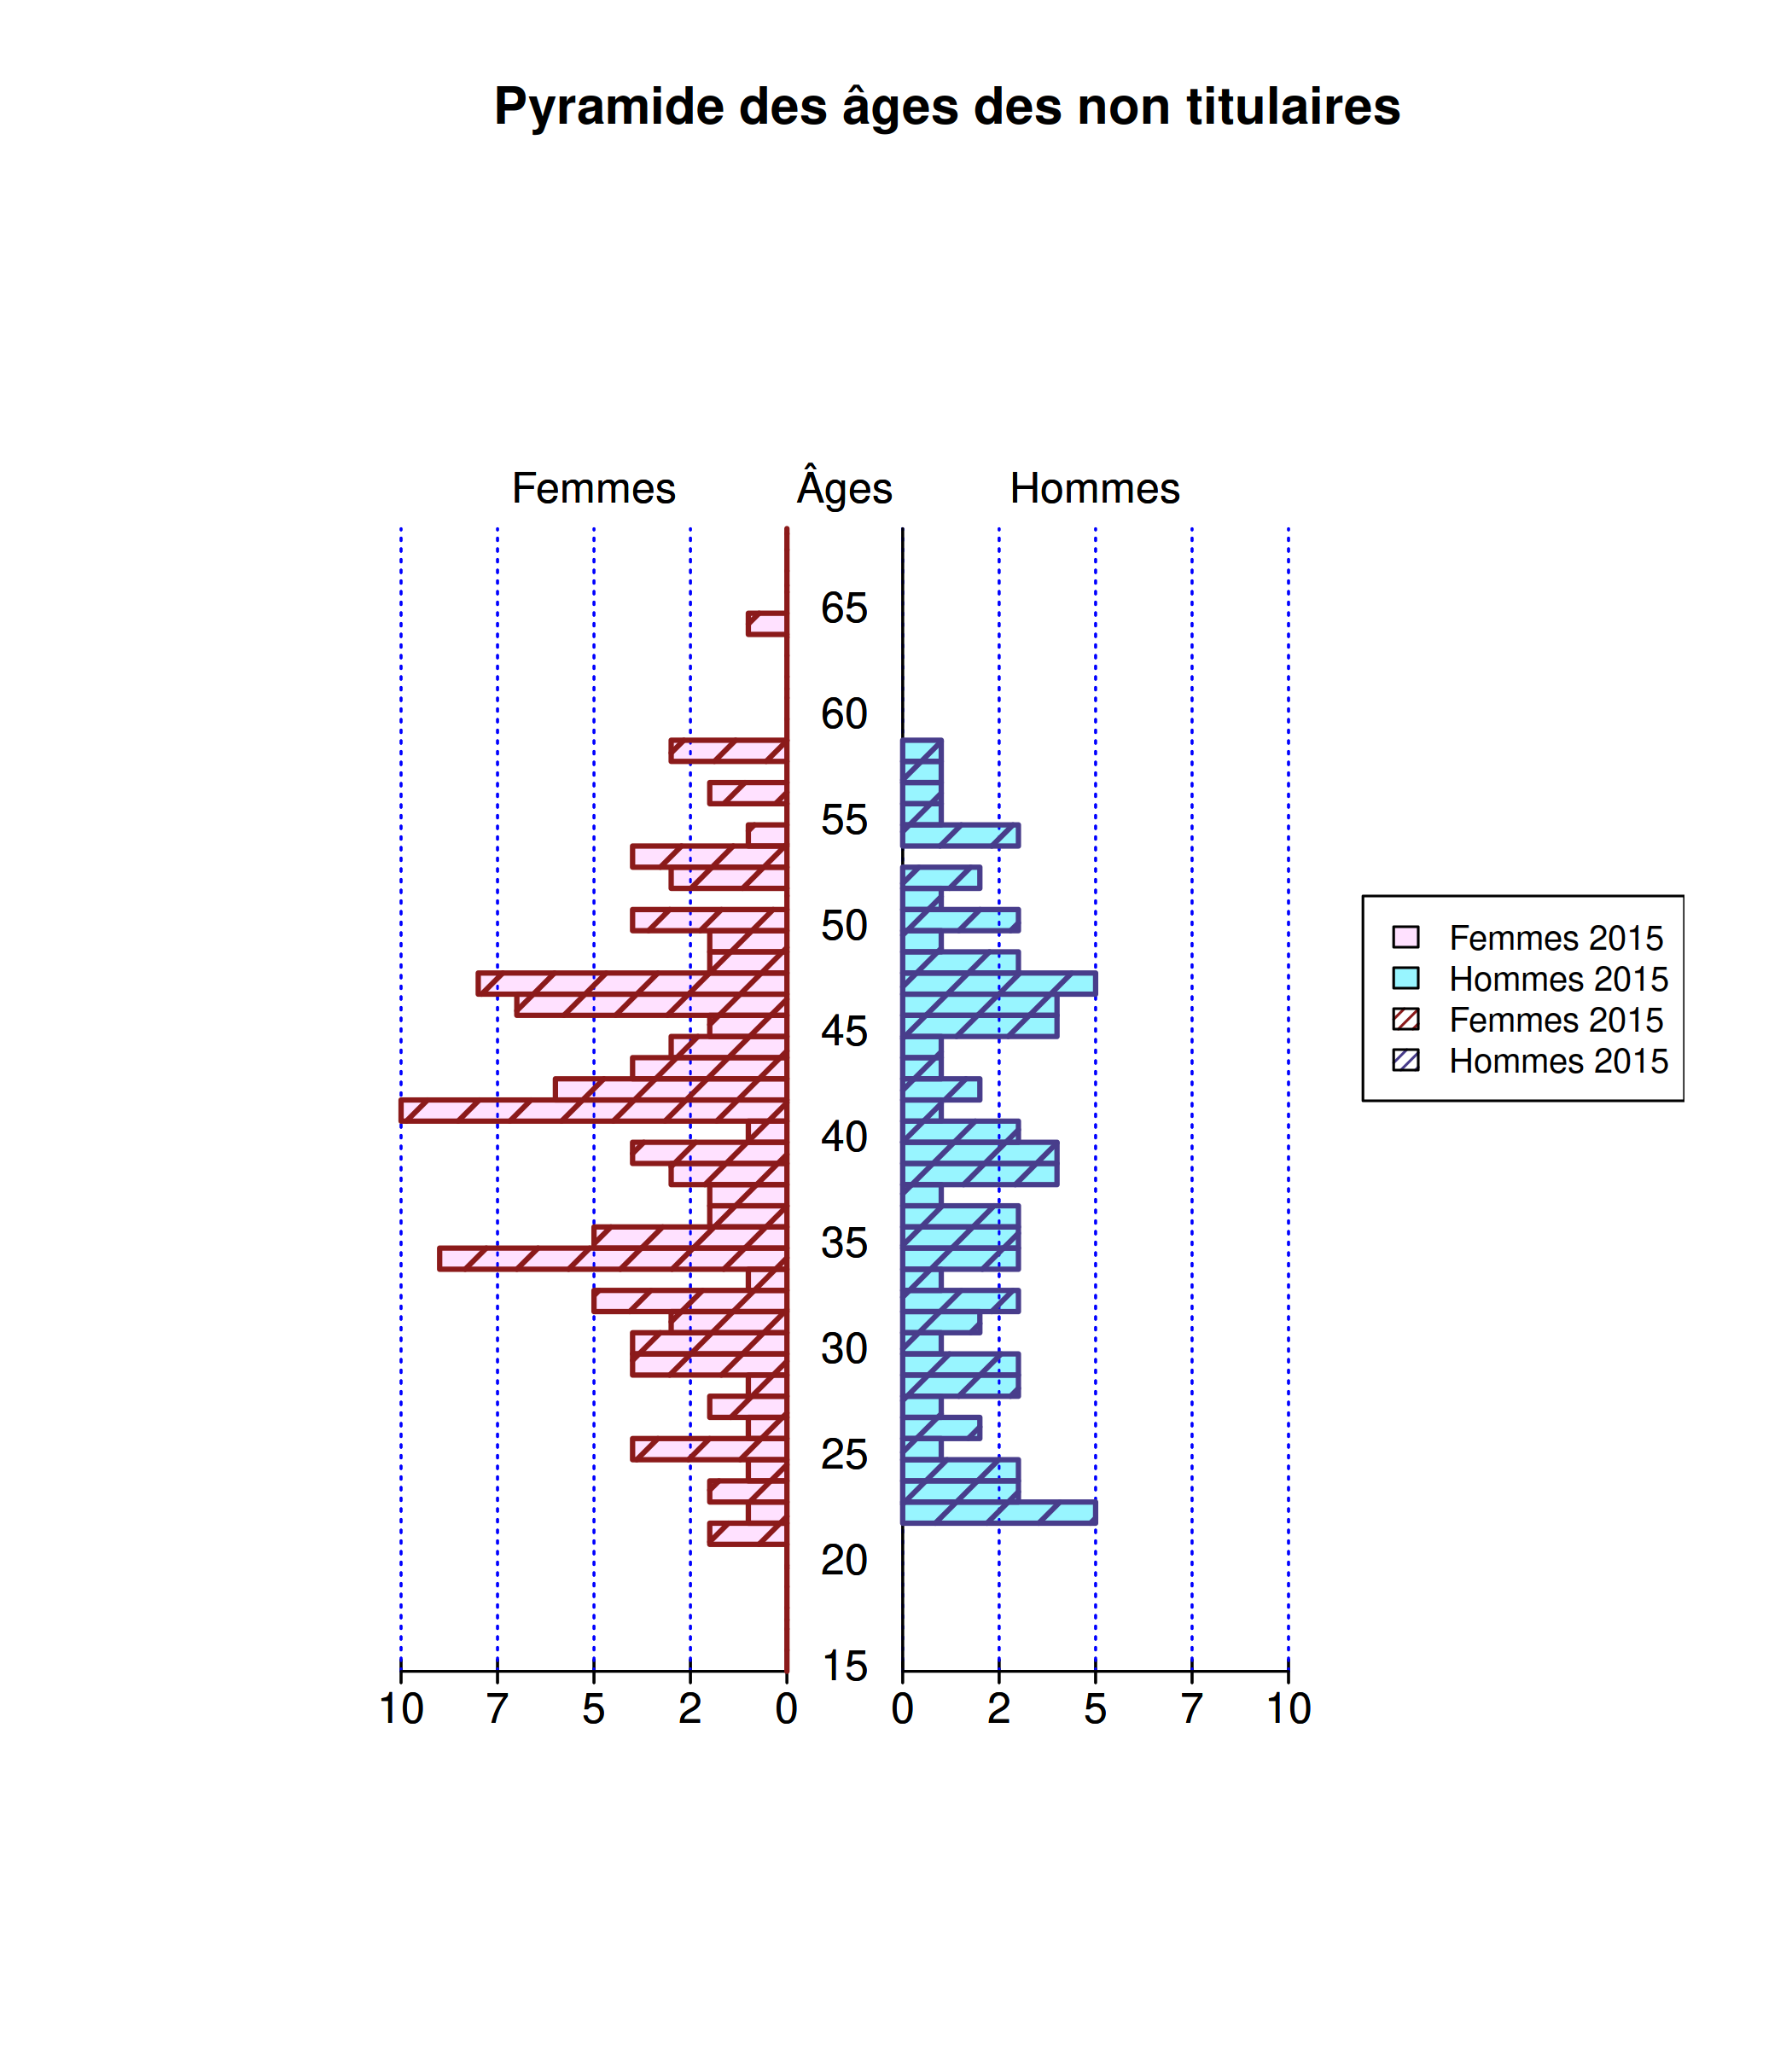
\includegraphics{altair_files/figure-latex/unnamed-chunk-23-1.png}
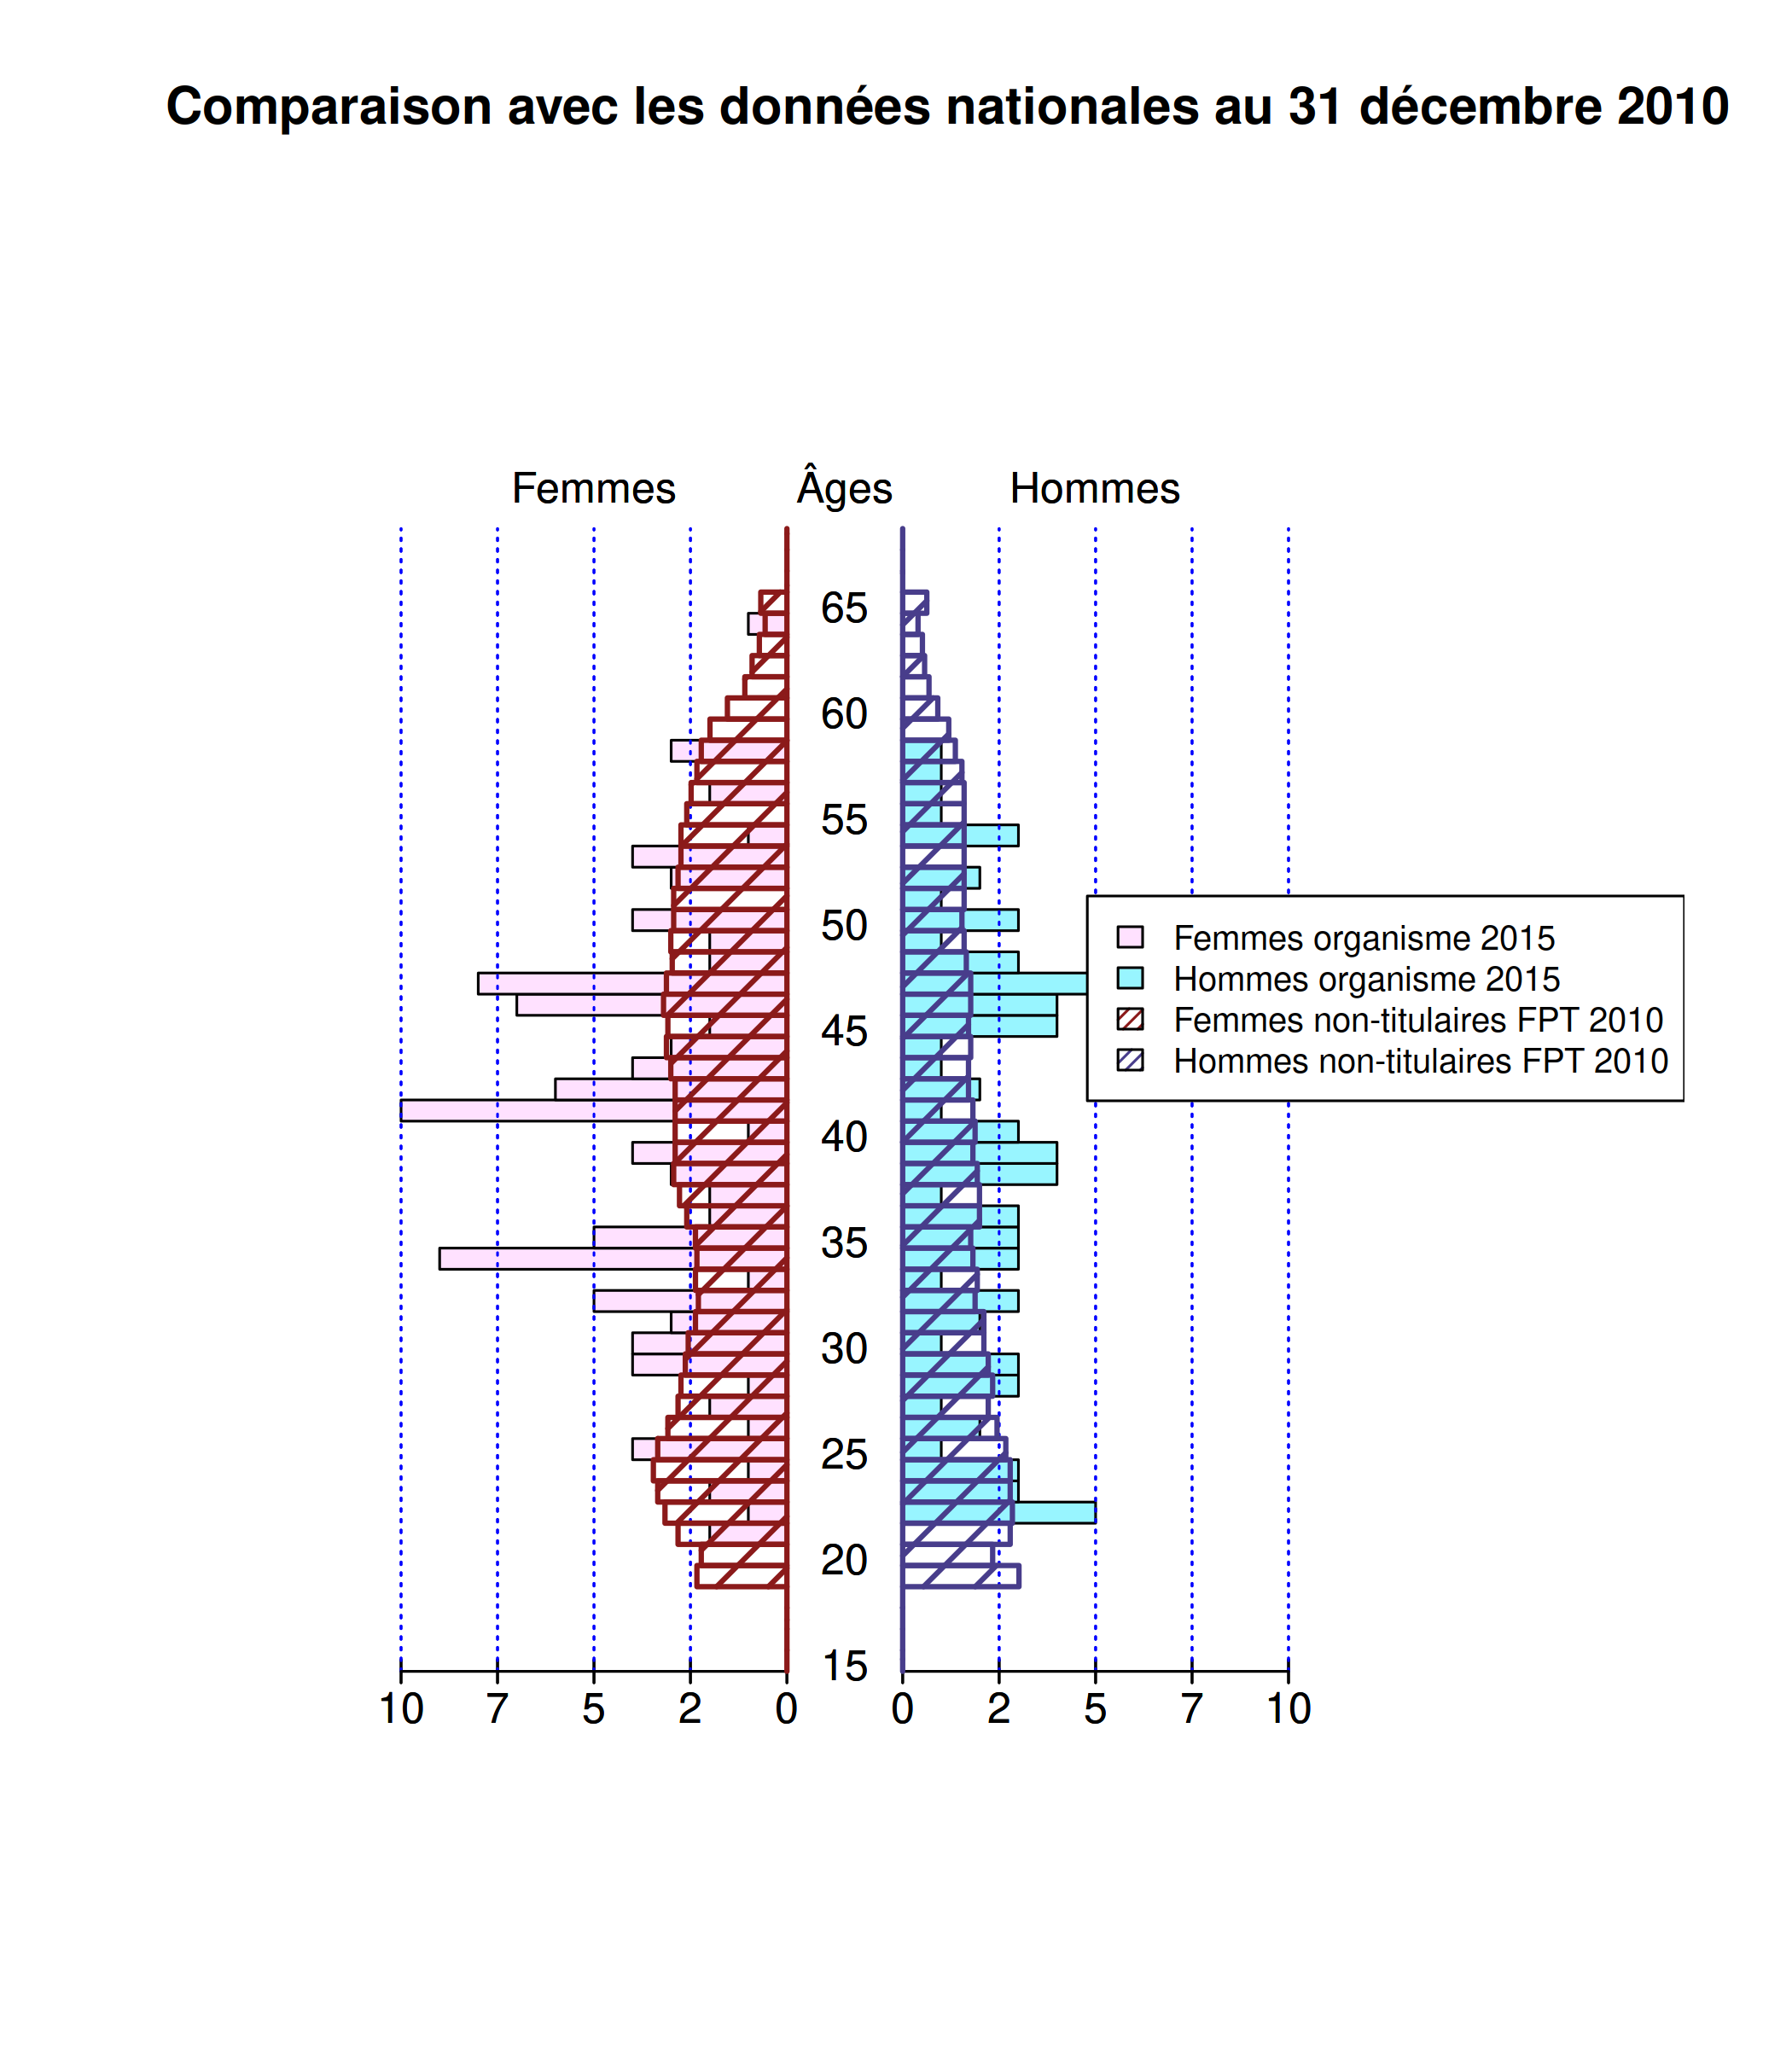
\includegraphics{altair_files/figure-latex/unnamed-chunk-23-2.png} Pour
obtenir les effectifs nationaux, multiplier les abscisses des hommes par
5 167 et les abscisses des femmes par 322\newpage
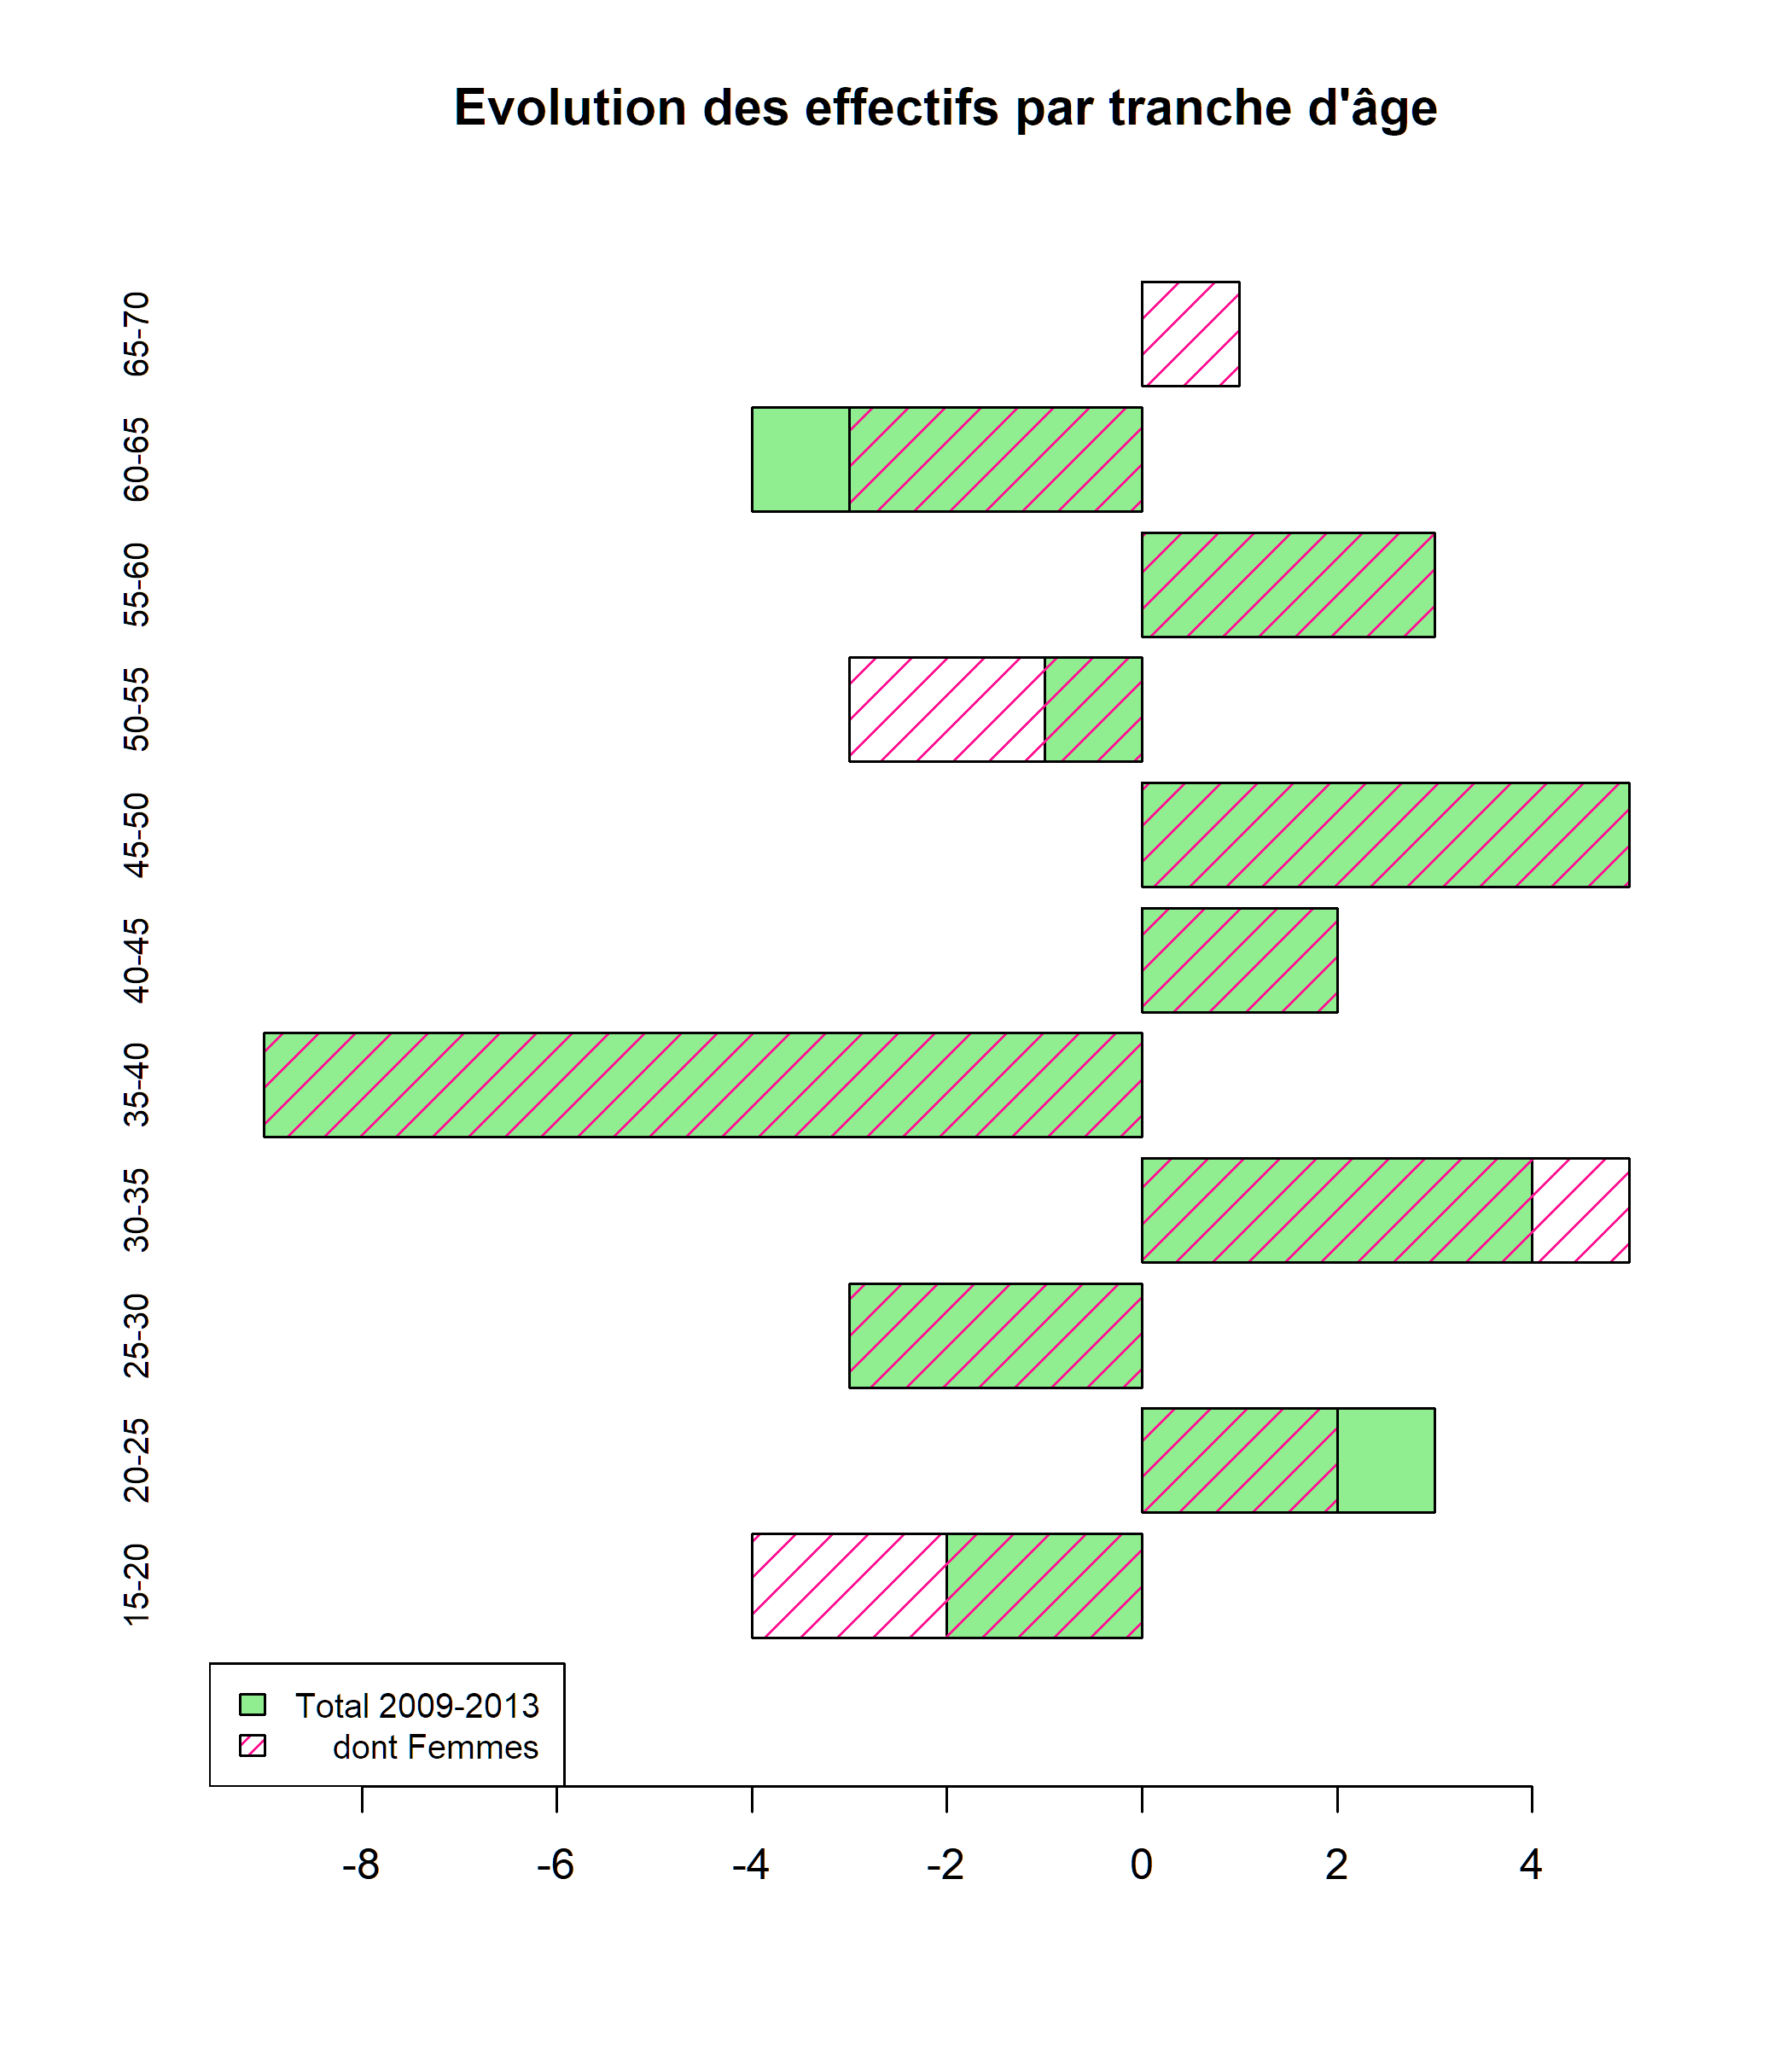
\includegraphics{altair_files/figure-latex/unnamed-chunk-23-3.png}

\href{../Docs/Notices/fiche_3.odt}{
\includegraphics{icones/Notice.png}}

\newpage

~\emph{Tableau 1.4.1}

\begin{longtable}[]{@{}ccccc@{}}
\toprule
\begin{minipage}[b]{0.12\columnwidth}\centering
Statistique\strut
\end{minipage} & \begin{minipage}[b]{0.29\columnwidth}\centering
Âge des personnels au 31/12/2011\strut
\end{minipage} & \begin{minipage}[b]{0.08\columnwidth}\centering
Effectif\strut
\end{minipage} & \begin{minipage}[b]{0.29\columnwidth}\centering
Âge des personnels au 31/12/2014\strut
\end{minipage} & \begin{minipage}[b]{0.08\columnwidth}\centering
Effectif\strut
\end{minipage}\tabularnewline
\midrule
\endhead
\begin{minipage}[t]{0.12\columnwidth}\centering
Minimum\strut
\end{minipage} & \begin{minipage}[t]{0.29\columnwidth}\centering
18,0\strut
\end{minipage} & \begin{minipage}[t]{0.08\columnwidth}\centering
\strut
\end{minipage} & \begin{minipage}[t]{0.29\columnwidth}\centering
18,0\strut
\end{minipage} & \begin{minipage}[t]{0.08\columnwidth}\centering
\strut
\end{minipage}\tabularnewline
\begin{minipage}[t]{0.12\columnwidth}\centering
1er quartile\strut
\end{minipage} & \begin{minipage}[t]{0.29\columnwidth}\centering
24,0\strut
\end{minipage} & \begin{minipage}[t]{0.08\columnwidth}\centering
\strut
\end{minipage} & \begin{minipage}[t]{0.29\columnwidth}\centering
24,0\strut
\end{minipage} & \begin{minipage}[t]{0.08\columnwidth}\centering
\strut
\end{minipage}\tabularnewline
\begin{minipage}[t]{0.12\columnwidth}\centering
Médiane\strut
\end{minipage} & \begin{minipage}[t]{0.29\columnwidth}\centering
27,0\strut
\end{minipage} & \begin{minipage}[t]{0.08\columnwidth}\centering
\strut
\end{minipage} & \begin{minipage}[t]{0.29\columnwidth}\centering
28,0\strut
\end{minipage} & \begin{minipage}[t]{0.08\columnwidth}\centering
\strut
\end{minipage}\tabularnewline
\begin{minipage}[t]{0.12\columnwidth}\centering
Moyenne\strut
\end{minipage} & \begin{minipage}[t]{0.29\columnwidth}\centering
31,9\strut
\end{minipage} & \begin{minipage}[t]{0.08\columnwidth}\centering
180\strut
\end{minipage} & \begin{minipage}[t]{0.29\columnwidth}\centering
32,0\strut
\end{minipage} & \begin{minipage}[t]{0.08\columnwidth}\centering
207\strut
\end{minipage}\tabularnewline
\begin{minipage}[t]{0.12\columnwidth}\centering
3ème quartile\strut
\end{minipage} & \begin{minipage}[t]{0.29\columnwidth}\centering
39,0\strut
\end{minipage} & \begin{minipage}[t]{0.08\columnwidth}\centering
\strut
\end{minipage} & \begin{minipage}[t]{0.29\columnwidth}\centering
38,5\strut
\end{minipage} & \begin{minipage}[t]{0.08\columnwidth}\centering
\strut
\end{minipage}\tabularnewline
\begin{minipage}[t]{0.12\columnwidth}\centering
Maximum\strut
\end{minipage} & \begin{minipage}[t]{0.29\columnwidth}\centering
61,0\strut
\end{minipage} & \begin{minipage}[t]{0.08\columnwidth}\centering
\strut
\end{minipage} & \begin{minipage}[t]{0.29\columnwidth}\centering
65,0\strut
\end{minipage} & \begin{minipage}[t]{0.08\columnwidth}\centering
\strut
\end{minipage}\tabularnewline
\bottomrule
\end{longtable}

\href{../Bases/Effectifs/Pyramide-des-ages-des-non-titulaires_2011.csv}{Lien
vers la base des âges - début de periode}

\href{../Bases/Effectifs/Pyramide-des-ages-des-non-titulaires_2014.csv}{Lien
vers la base des âges - fin de periode}

\href{../Docs/Notices/fiche_1.odt}{
\includegraphics{icones/Notice.png}}

\hypertarget{pyramide-des-ages-autres-statuts}{%
\subsection{1.5 Pyramide des âges, autres statuts
~}\label{pyramide-des-ages-autres-statuts}}

\href{../Docs/Notices/fiche_2.odt}{
\includegraphics{icones/Notice.png}}

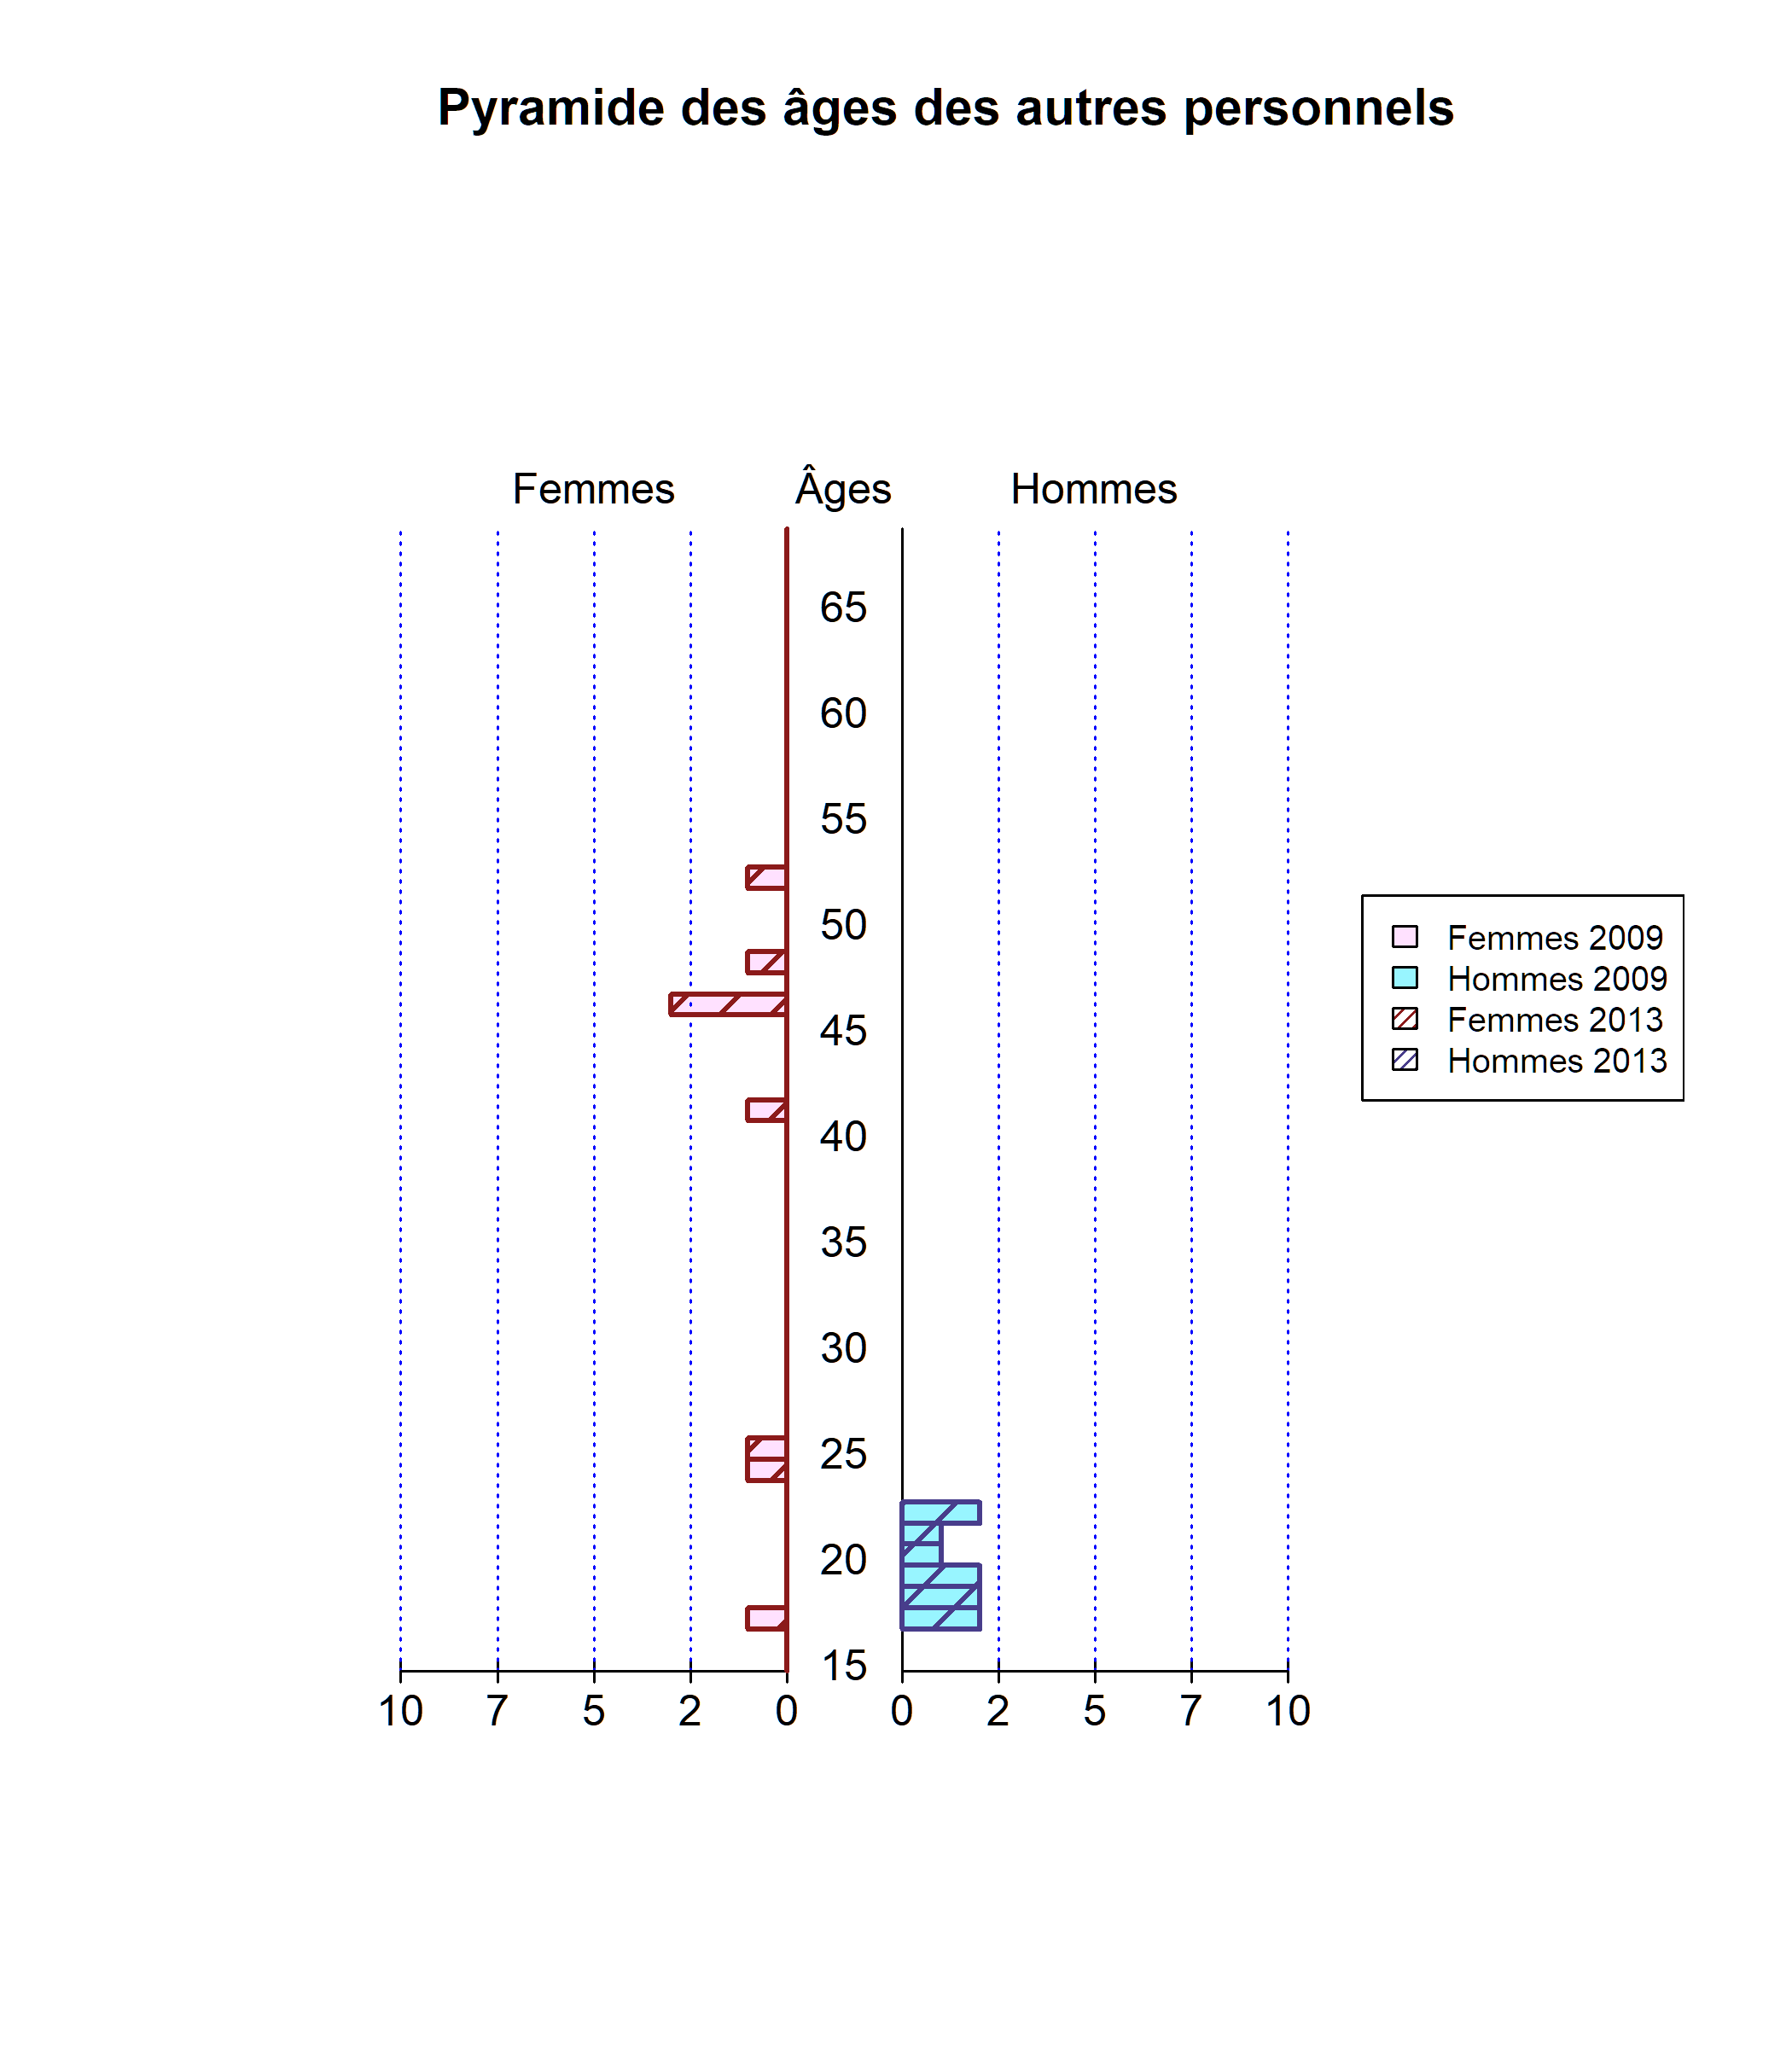
\includegraphics{altair_files/figure-latex/unnamed-chunk-29-1.png}
\newpage
\includegraphics{altair_files/figure-latex/unnamed-chunk-29-2.png}

\href{../Docs/Notices/fiche_3.odt}{
\includegraphics{icones/Notice.png}}

\newpage

~\emph{Tableau 1.5.1}

\begin{longtable}[]{@{}ccccc@{}}
\toprule
\begin{minipage}[b]{0.12\columnwidth}\centering
Statistique\strut
\end{minipage} & \begin{minipage}[b]{0.29\columnwidth}\centering
Âge des personnels au 31/12/2011\strut
\end{minipage} & \begin{minipage}[b]{0.08\columnwidth}\centering
Effectif\strut
\end{minipage} & \begin{minipage}[b]{0.29\columnwidth}\centering
Âge des personnels au 31/12/2014\strut
\end{minipage} & \begin{minipage}[b]{0.08\columnwidth}\centering
Effectif\strut
\end{minipage}\tabularnewline
\midrule
\endhead
\begin{minipage}[t]{0.12\columnwidth}\centering
Minimum\strut
\end{minipage} & \begin{minipage}[t]{0.29\columnwidth}\centering
21,0\strut
\end{minipage} & \begin{minipage}[t]{0.08\columnwidth}\centering
\strut
\end{minipage} & \begin{minipage}[t]{0.29\columnwidth}\centering
19,0\strut
\end{minipage} & \begin{minipage}[t]{0.08\columnwidth}\centering
\strut
\end{minipage}\tabularnewline
\begin{minipage}[t]{0.12\columnwidth}\centering
1er quartile\strut
\end{minipage} & \begin{minipage}[t]{0.29\columnwidth}\centering
24,0\strut
\end{minipage} & \begin{minipage}[t]{0.08\columnwidth}\centering
\strut
\end{minipage} & \begin{minipage}[t]{0.29\columnwidth}\centering
27,0\strut
\end{minipage} & \begin{minipage}[t]{0.08\columnwidth}\centering
\strut
\end{minipage}\tabularnewline
\begin{minipage}[t]{0.12\columnwidth}\centering
Médiane\strut
\end{minipage} & \begin{minipage}[t]{0.29\columnwidth}\centering
33,5\strut
\end{minipage} & \begin{minipage}[t]{0.08\columnwidth}\centering
\strut
\end{minipage} & \begin{minipage}[t]{0.29\columnwidth}\centering
39,0\strut
\end{minipage} & \begin{minipage}[t]{0.08\columnwidth}\centering
\strut
\end{minipage}\tabularnewline
\begin{minipage}[t]{0.12\columnwidth}\centering
Moyenne\strut
\end{minipage} & \begin{minipage}[t]{0.29\columnwidth}\centering
37,7\strut
\end{minipage} & \begin{minipage}[t]{0.08\columnwidth}\centering
134\strut
\end{minipage} & \begin{minipage}[t]{0.29\columnwidth}\centering
40,1\strut
\end{minipage} & \begin{minipage}[t]{0.08\columnwidth}\centering
151\strut
\end{minipage}\tabularnewline
\begin{minipage}[t]{0.12\columnwidth}\centering
3ème quartile\strut
\end{minipage} & \begin{minipage}[t]{0.29\columnwidth}\centering
49,8\strut
\end{minipage} & \begin{minipage}[t]{0.08\columnwidth}\centering
\strut
\end{minipage} & \begin{minipage}[t]{0.29\columnwidth}\centering
53,0\strut
\end{minipage} & \begin{minipage}[t]{0.08\columnwidth}\centering
\strut
\end{minipage}\tabularnewline
\begin{minipage}[t]{0.12\columnwidth}\centering
Maximum\strut
\end{minipage} & \begin{minipage}[t]{0.29\columnwidth}\centering
74,0\strut
\end{minipage} & \begin{minipage}[t]{0.08\columnwidth}\centering
\strut
\end{minipage} & \begin{minipage}[t]{0.29\columnwidth}\centering
72,0\strut
\end{minipage} & \begin{minipage}[t]{0.08\columnwidth}\centering
\strut
\end{minipage}\tabularnewline
\bottomrule
\end{longtable}

\href{../Bases/Effectifs/Pyramide-des-ages-des-autres-personnels_2011.csv}{Lien
vers la base des âges - début de periode}

\href{../Bases/Effectifs/Pyramide-des-ages-des-autres-personnels_2014.csv}{Lien
vers la base des âges - fin de periode}

\href{../Docs/Notices/fiche_1.odt}{
\includegraphics{icones/Notice.png}}

\emph{Source des comparaisons avec les données nationales}

Rapport annuel sur l'état de la fonction publique pour 2016\\
\href{../Docs/insee_pyramide_fph_2013.csv}{Pyramide 2013 FPH}\\
\href{../Docs/insee_pyramide_fpt_2013.csv}{Pyramide 2013 FPT}\\
\emph{Toutes les pyramides des âges sont établies au 31 décembre de
l'annee considérée.}\\
\emph{Les élus ne sont pas compris dans le périmètre statistique.}

\hypertarget{effectifs-des-personnels-par-duree-de-service}{%
\subsection{1.6 Effectifs des personnels par duree de
service}\label{effectifs-des-personnels-par-duree-de-service}}

\textbf{Personnels en fonction (hors élus) des exercices 2011 à 2014
inclus :}

~\emph{Tableau 1.6.1}

\begin{longtable}[]{@{}cccc@{}}
\toprule
Plus de 2 ans & Moins de 2 ans & Moins d'un an & Moins de six
mois\tabularnewline
\midrule
\endhead
0 & 3 840 & 3 840 & 3 840\tabularnewline
\bottomrule
\end{longtable}

\textbf{Effectifs (hors élus)}

~\emph{Tableau 1.6.2}

\begin{longtable}[]{@{}lcccc@{}}
\toprule
& 2011 & 2012 & 2013 & 2014\tabularnewline
\midrule
\endhead
Plus de deux ans & 0 & 0 & 0 & 0\tabularnewline
Moins de deux ans & 922 & 970 & 970 & 978\tabularnewline
Total & 922 & 970 & 970 & 978\tabularnewline
\bottomrule
\end{longtable}

\textbf{Nota :} \emph{Personnels en place : ayant servi au moins deux
années consécutives pendant la periode.}\\
\emph{Plus/moins de deux ans : plus/mois de 730 jours sur la periode
sous revue.}

\hypertarget{remunerations-brutes-analyse-pour-le-premier-exercice}{%
\section{2. Rémunérations brutes : analyse pour le premier
exercice}\label{remunerations-brutes-analyse-pour-le-premier-exercice}}

\textbf{Exercice : 2011 }

\hypertarget{remunerations-brutes-de-lensemble-des-agents}{%
\subsection{2.1 Rémunérations brutes de l'ensemble des
agents}\label{remunerations-brutes-de-lensemble-des-agents}}

\textbf{Cumuls des rémunérations brutes pour l'exercice 2011 }

\emph{Personnels (hors élus)}

~\emph{Tableau 2.1.1}

\begin{longtable}[]{@{}ll@{}}
\toprule
Agrégats & k€\tabularnewline
\midrule
\endhead
Brut annuel (bulletins) & 25 077 949,1\tabularnewline
Brut annuel (lignes) : & 25 335 757,4\tabularnewline
~dont ~Primes : & 2 898 777,0\tabularnewline
~dont ~Autres rémunérations &\tabularnewline
Part de primes en \% & 11,6\tabularnewline
\bottomrule
\end{longtable}

\textbf{Définitions :}

\emph{Brut annuel (bulletins)} : somme du champ \emph{Brut}\\
\emph{Brut annuel (lignes)} : somme du champ \emph{Montant} des lignes
de paye, dont :\\
\emph{Primes} : indemnités sauf remboursements, certaines IJSS,
indemnités d'élu le cas échéant, Supplément familial de traitement et
Indemnité de résidence\\
\emph{Autres rémunérations} : acomptes, retenues sur brut, rémunérations
diverses, rappels

\textbf{Tests de cohérence}

Somme des rémunérations brutes versées aux personnels (non élus) :

~\emph{Tableau 2.1.2}

\begin{longtable}[]{@{}ll@{}}
\toprule
Agrégats & k€\tabularnewline
\midrule
\endhead
Bulletins de paie & 25 077 949,1\tabularnewline
Lignes de paie & 25 335 757,4\tabularnewline
Difference & -257 808,3\tabularnewline
\bottomrule
\end{longtable}

à comparer aux soldes des comptes 641 et 648 du compte de gestion.

\hypertarget{remunerations-brutes-des-fonctionnaires}{%
\subsection{2.2 Rémunérations brutes des
fonctionnaires}\label{remunerations-brutes-des-fonctionnaires}}

\emph{Cette section concerne les personnels fonctionnaires titulaires et
stagiaires}

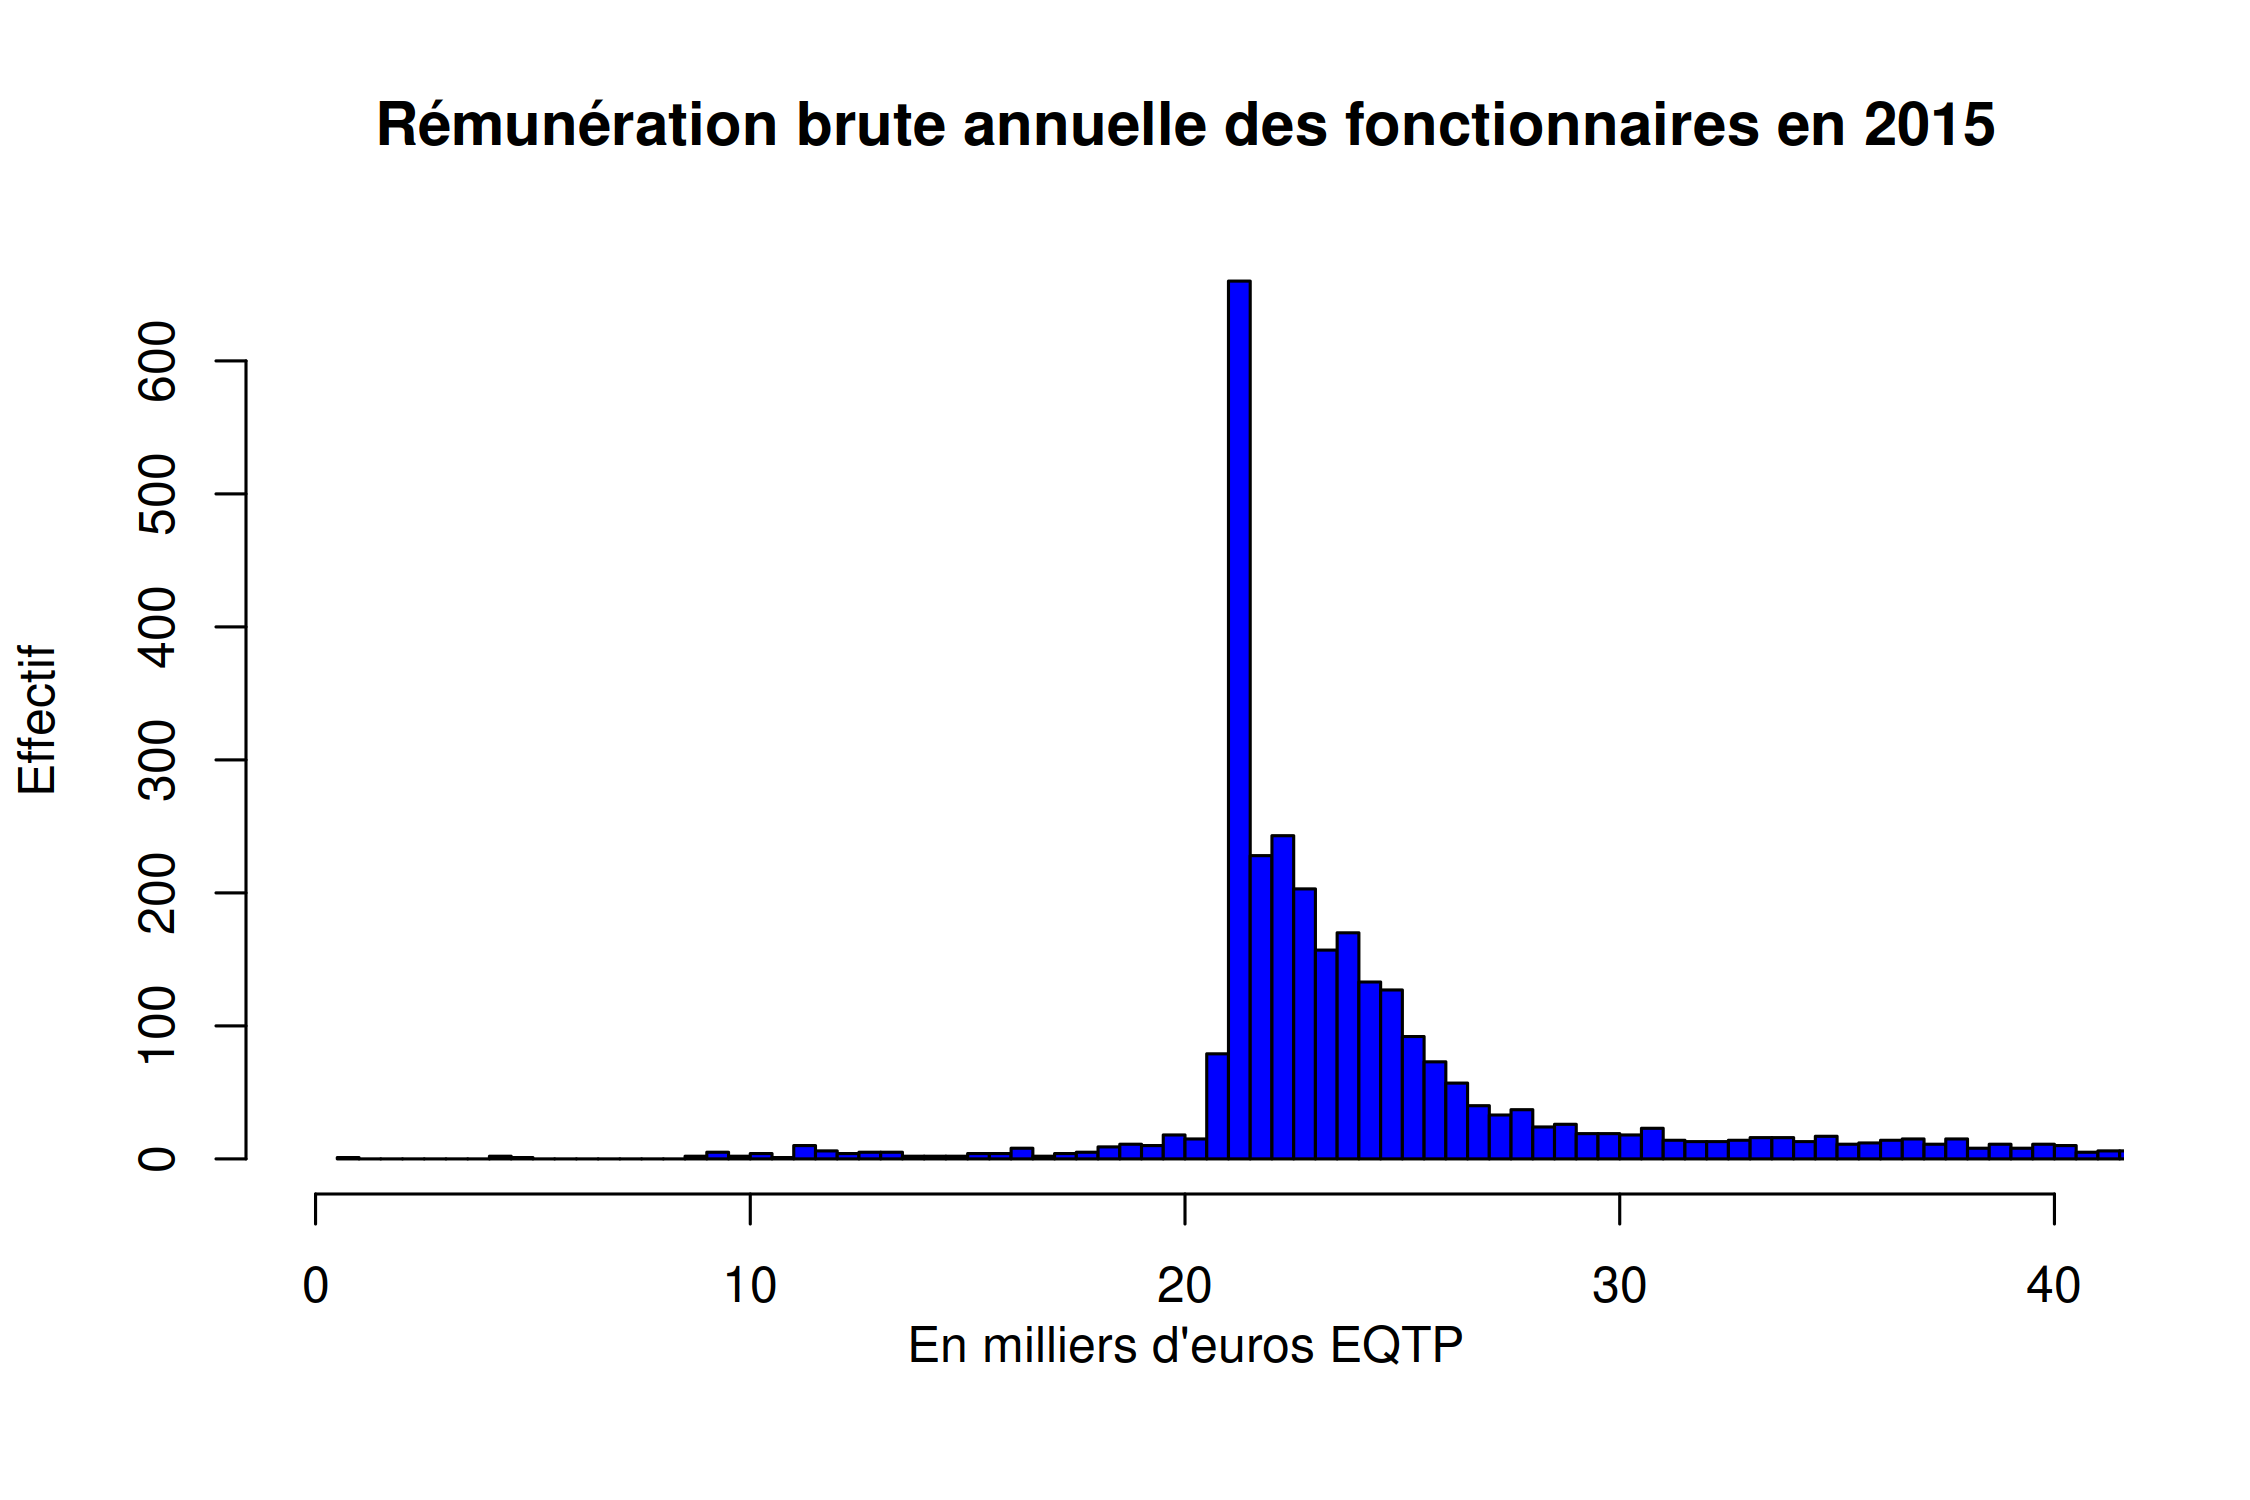
\includegraphics{altair_files/figure-latex/unnamed-chunk-43-1.png}

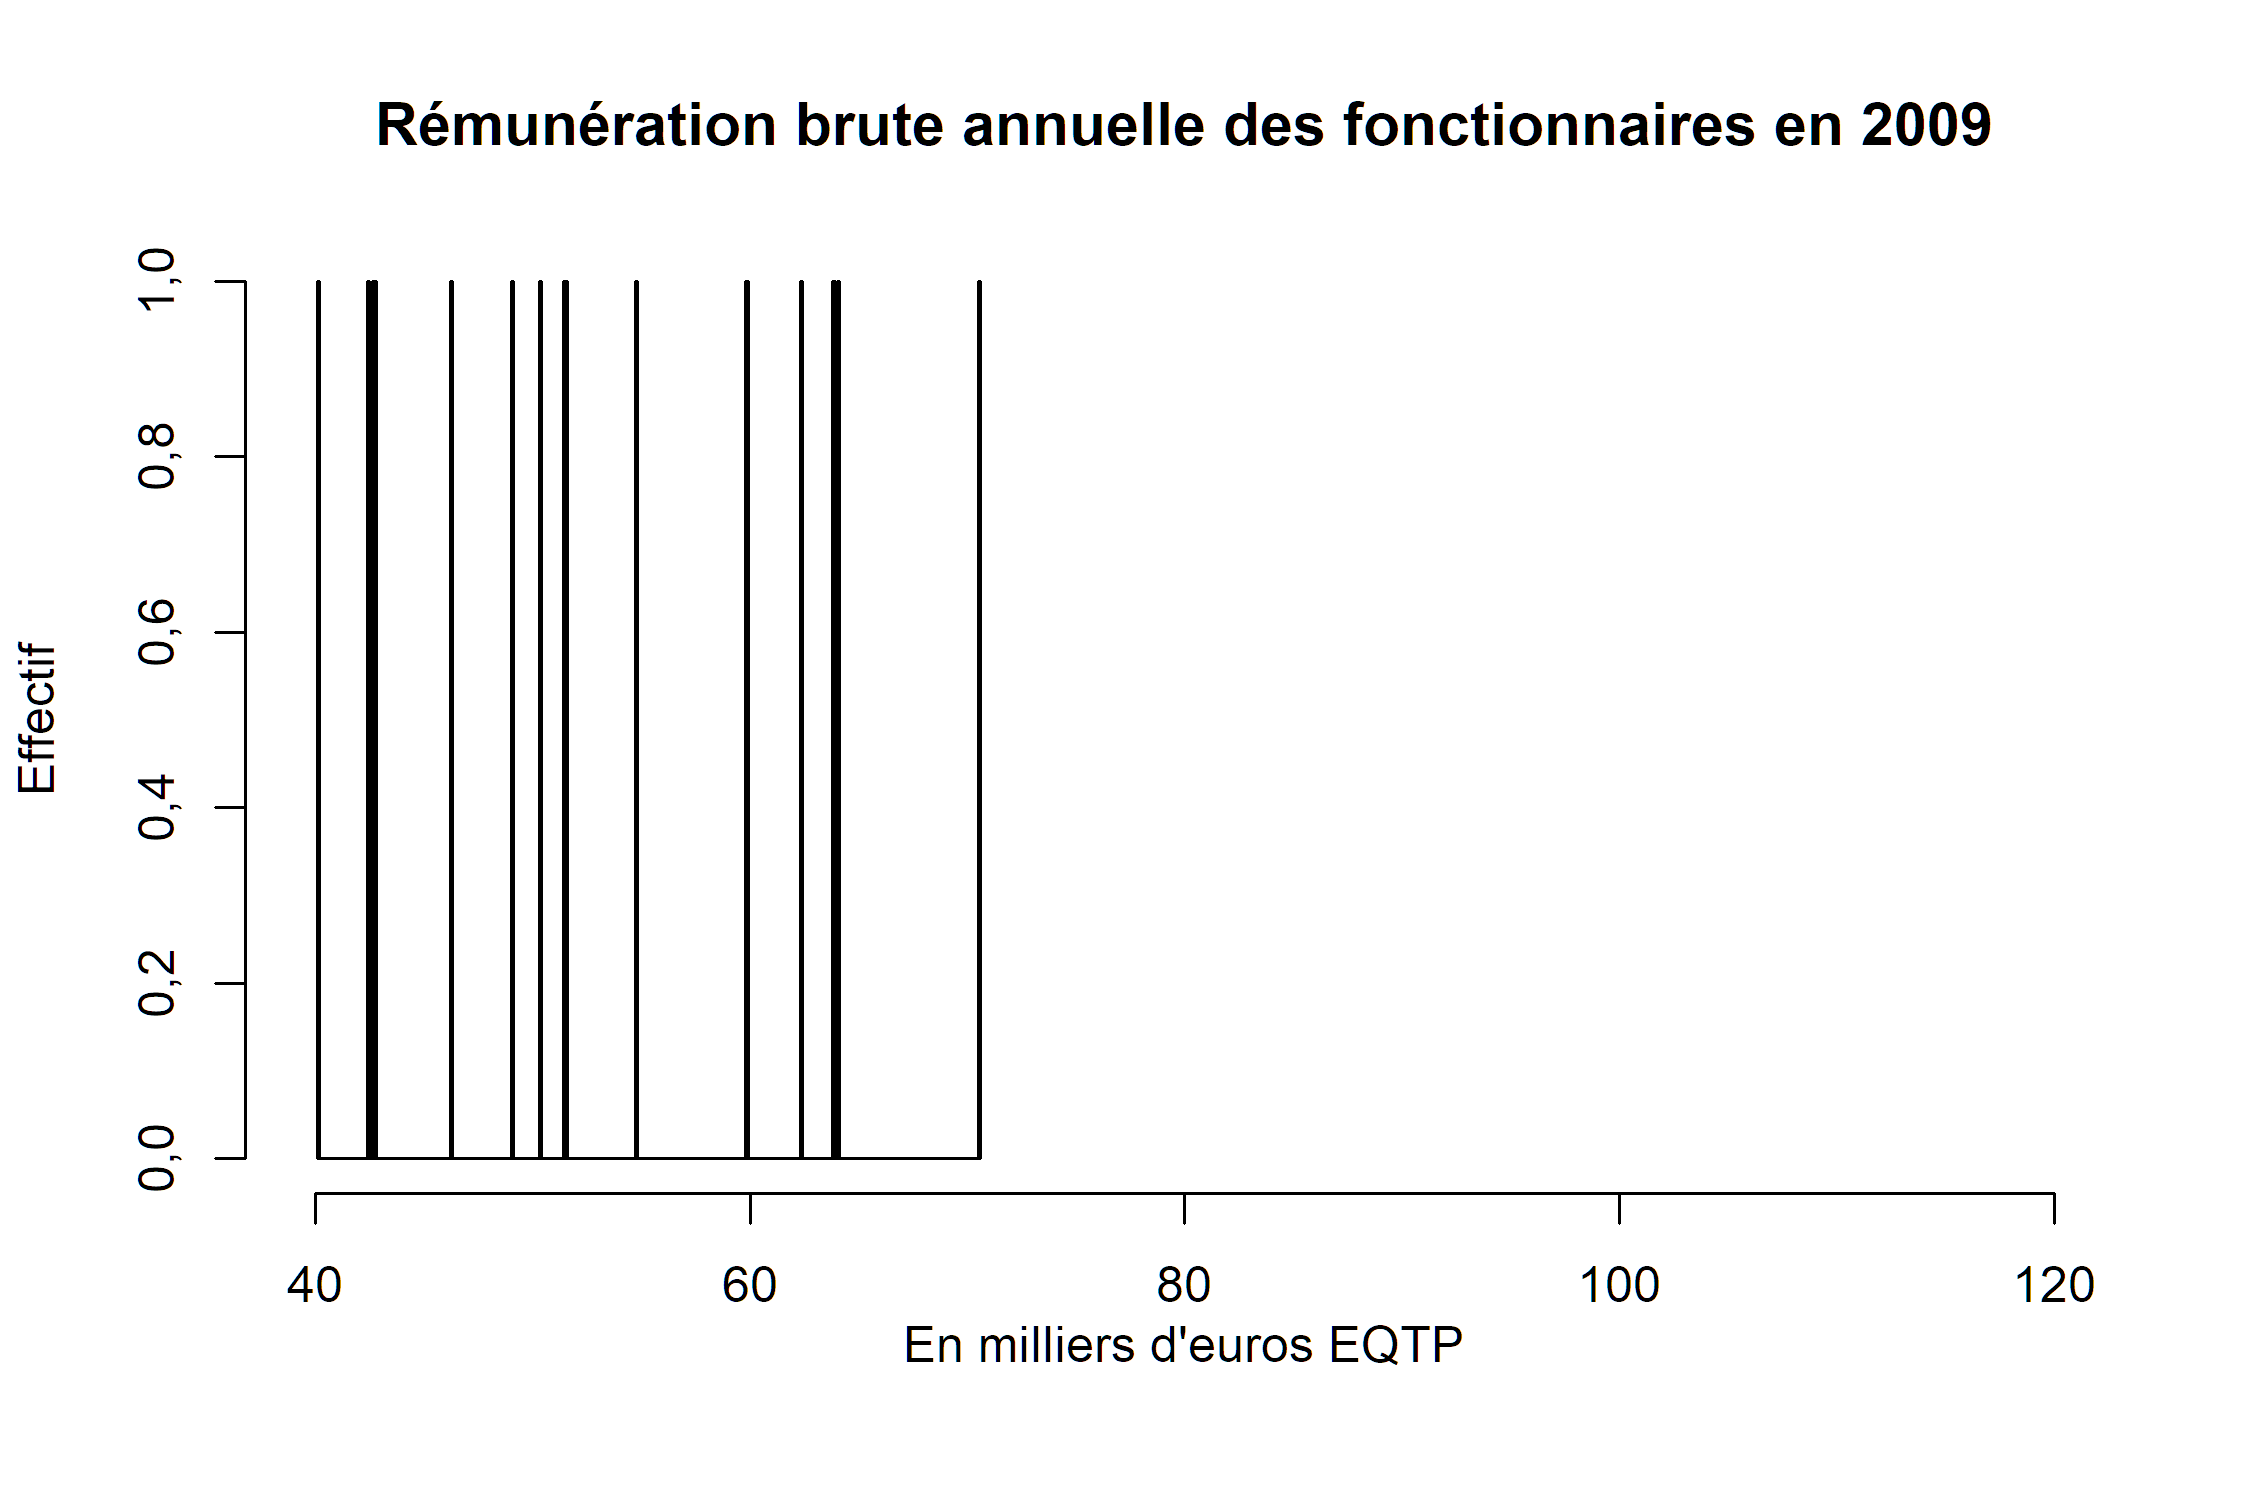
\includegraphics{altair_files/figure-latex/unnamed-chunk-43-2.png}

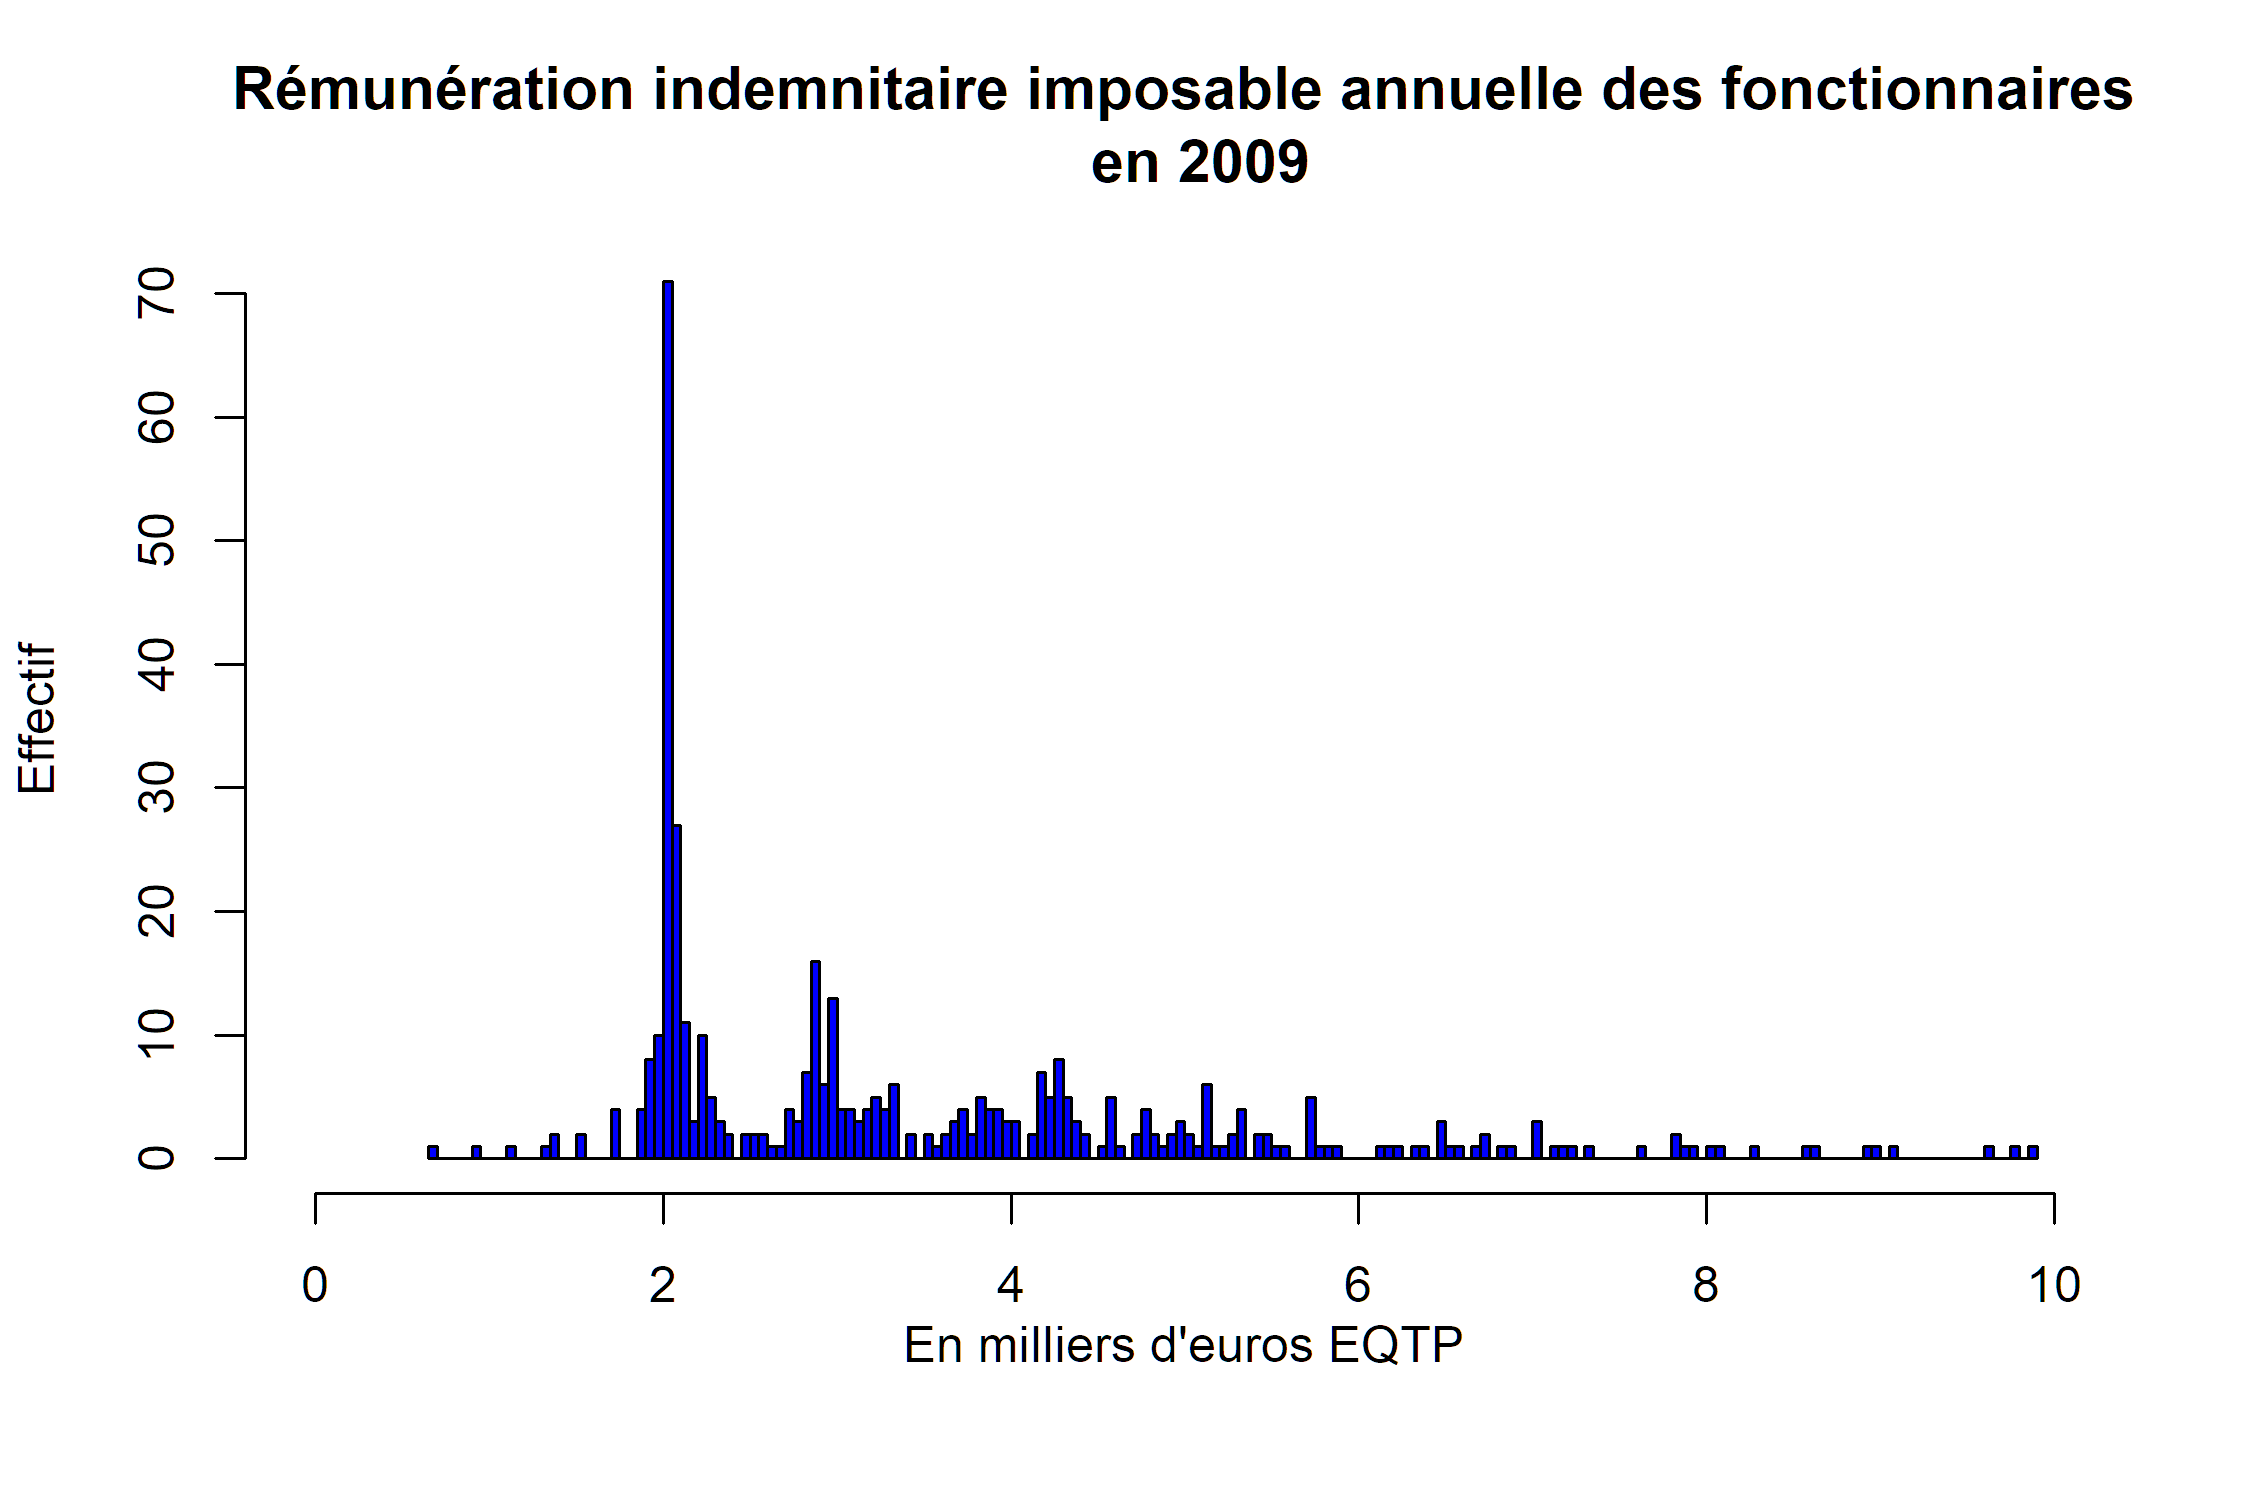
\includegraphics{altair_files/figure-latex/unnamed-chunk-43-3.png}

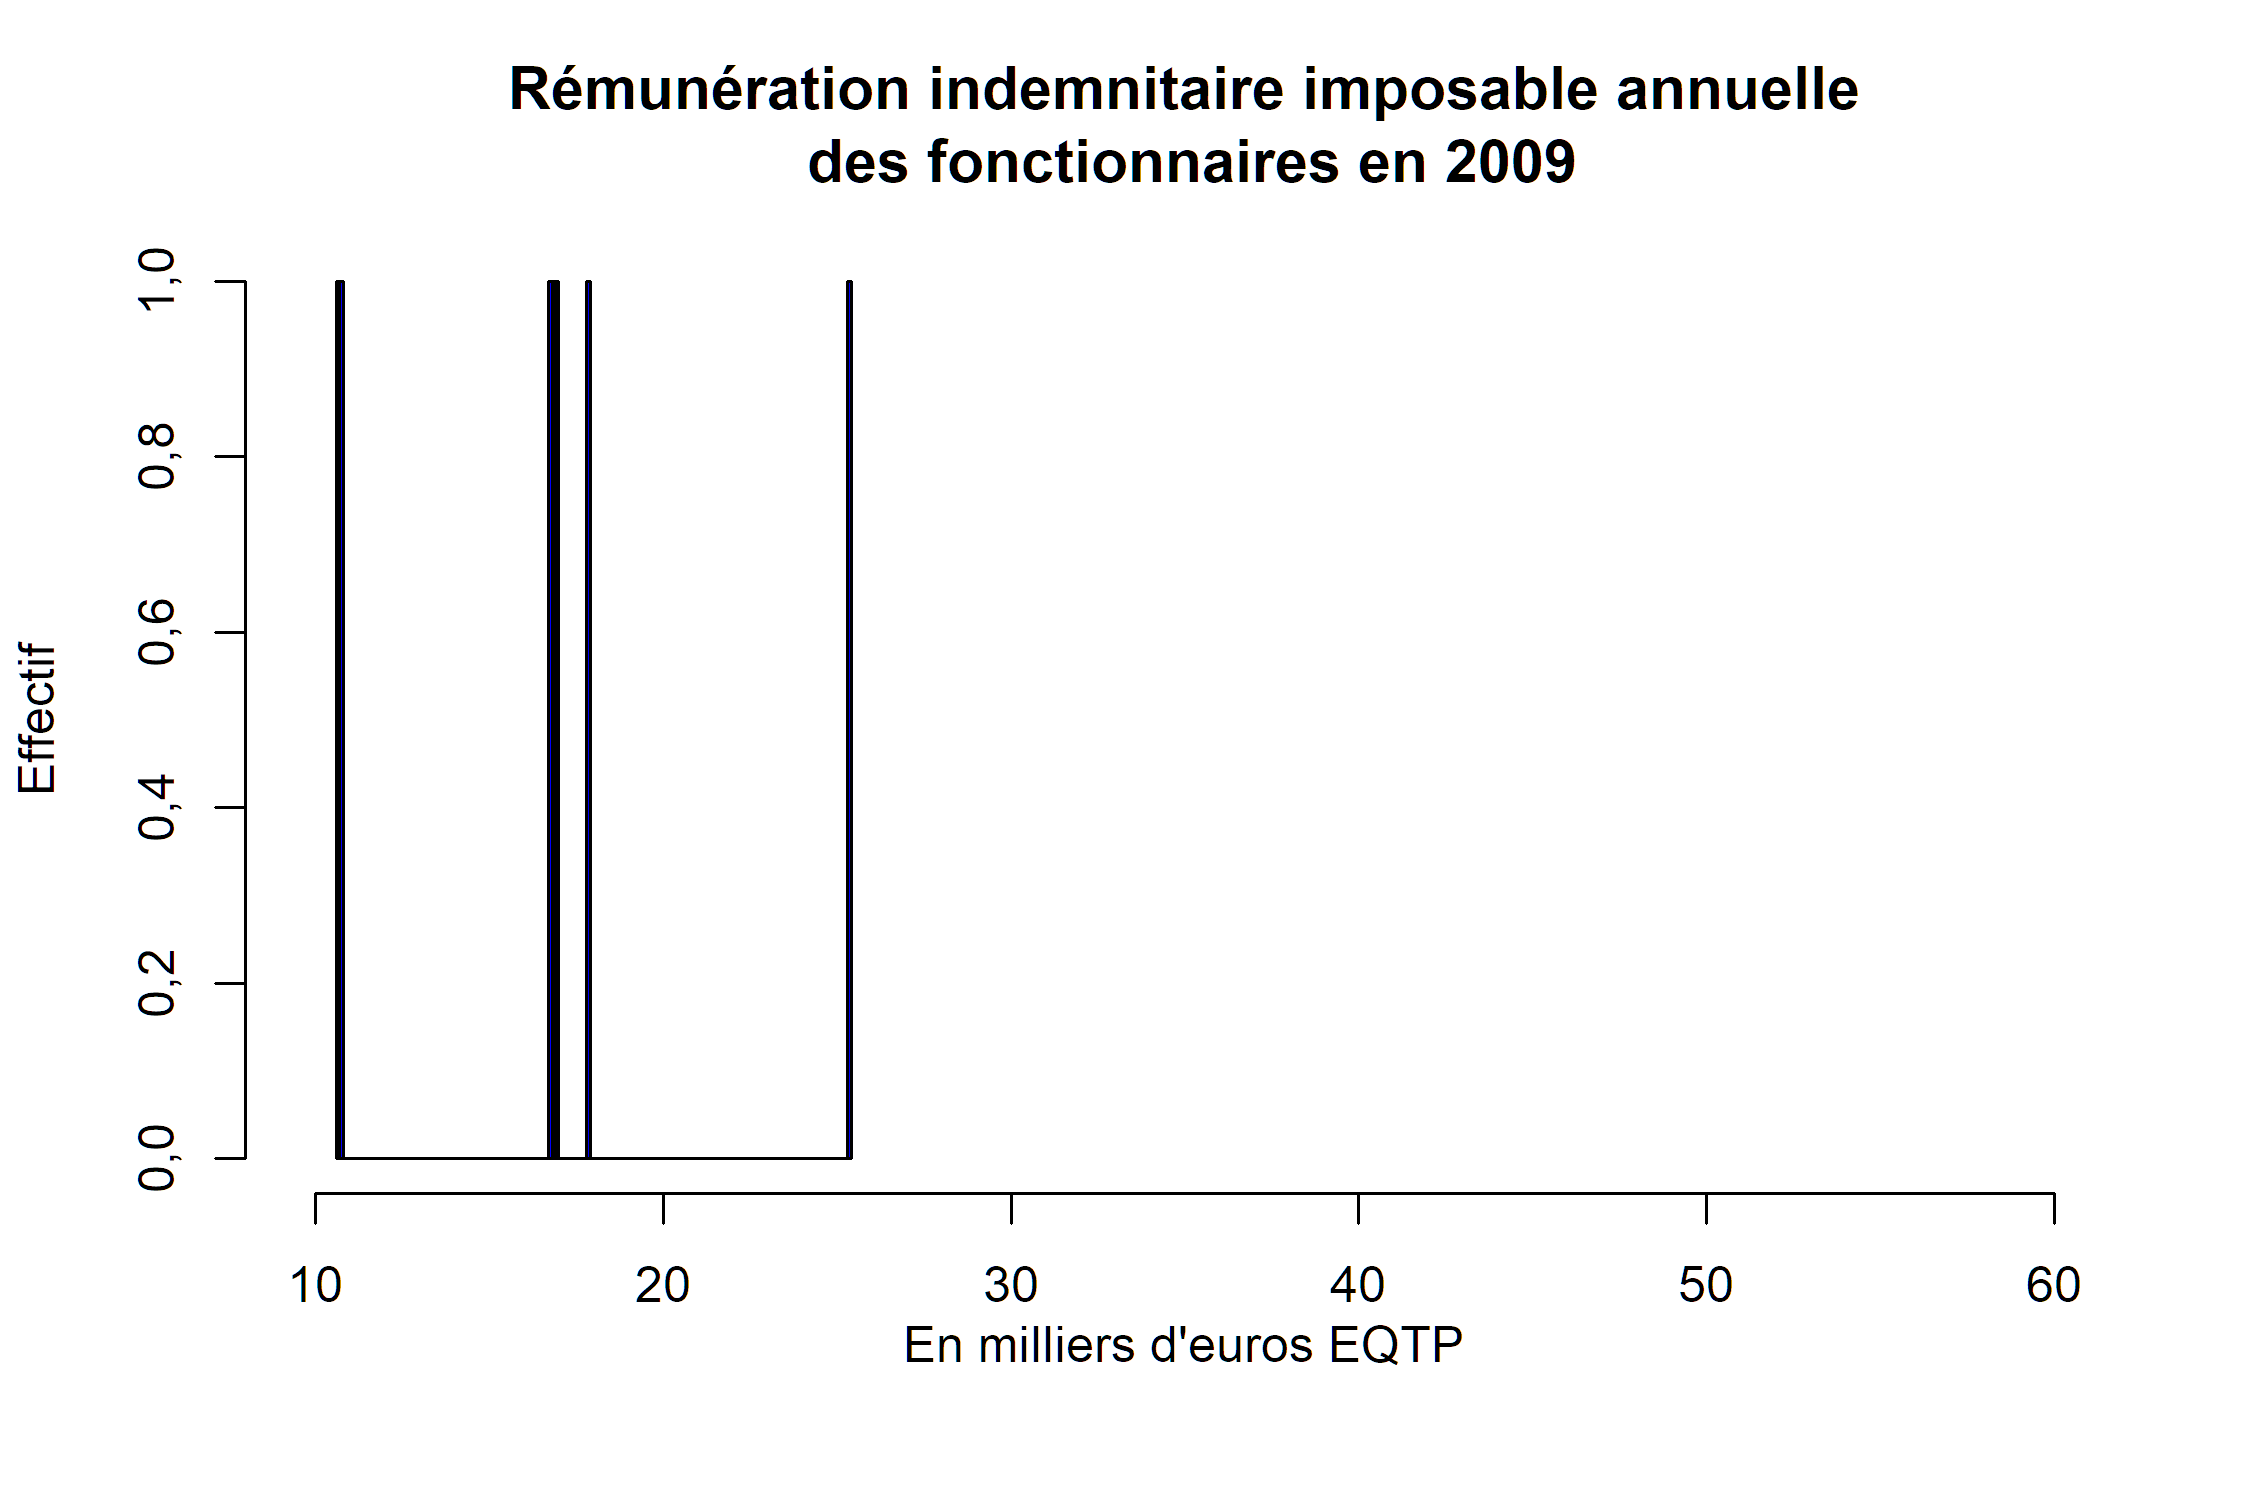
\includegraphics{altair_files/figure-latex/unnamed-chunk-43-4.png}

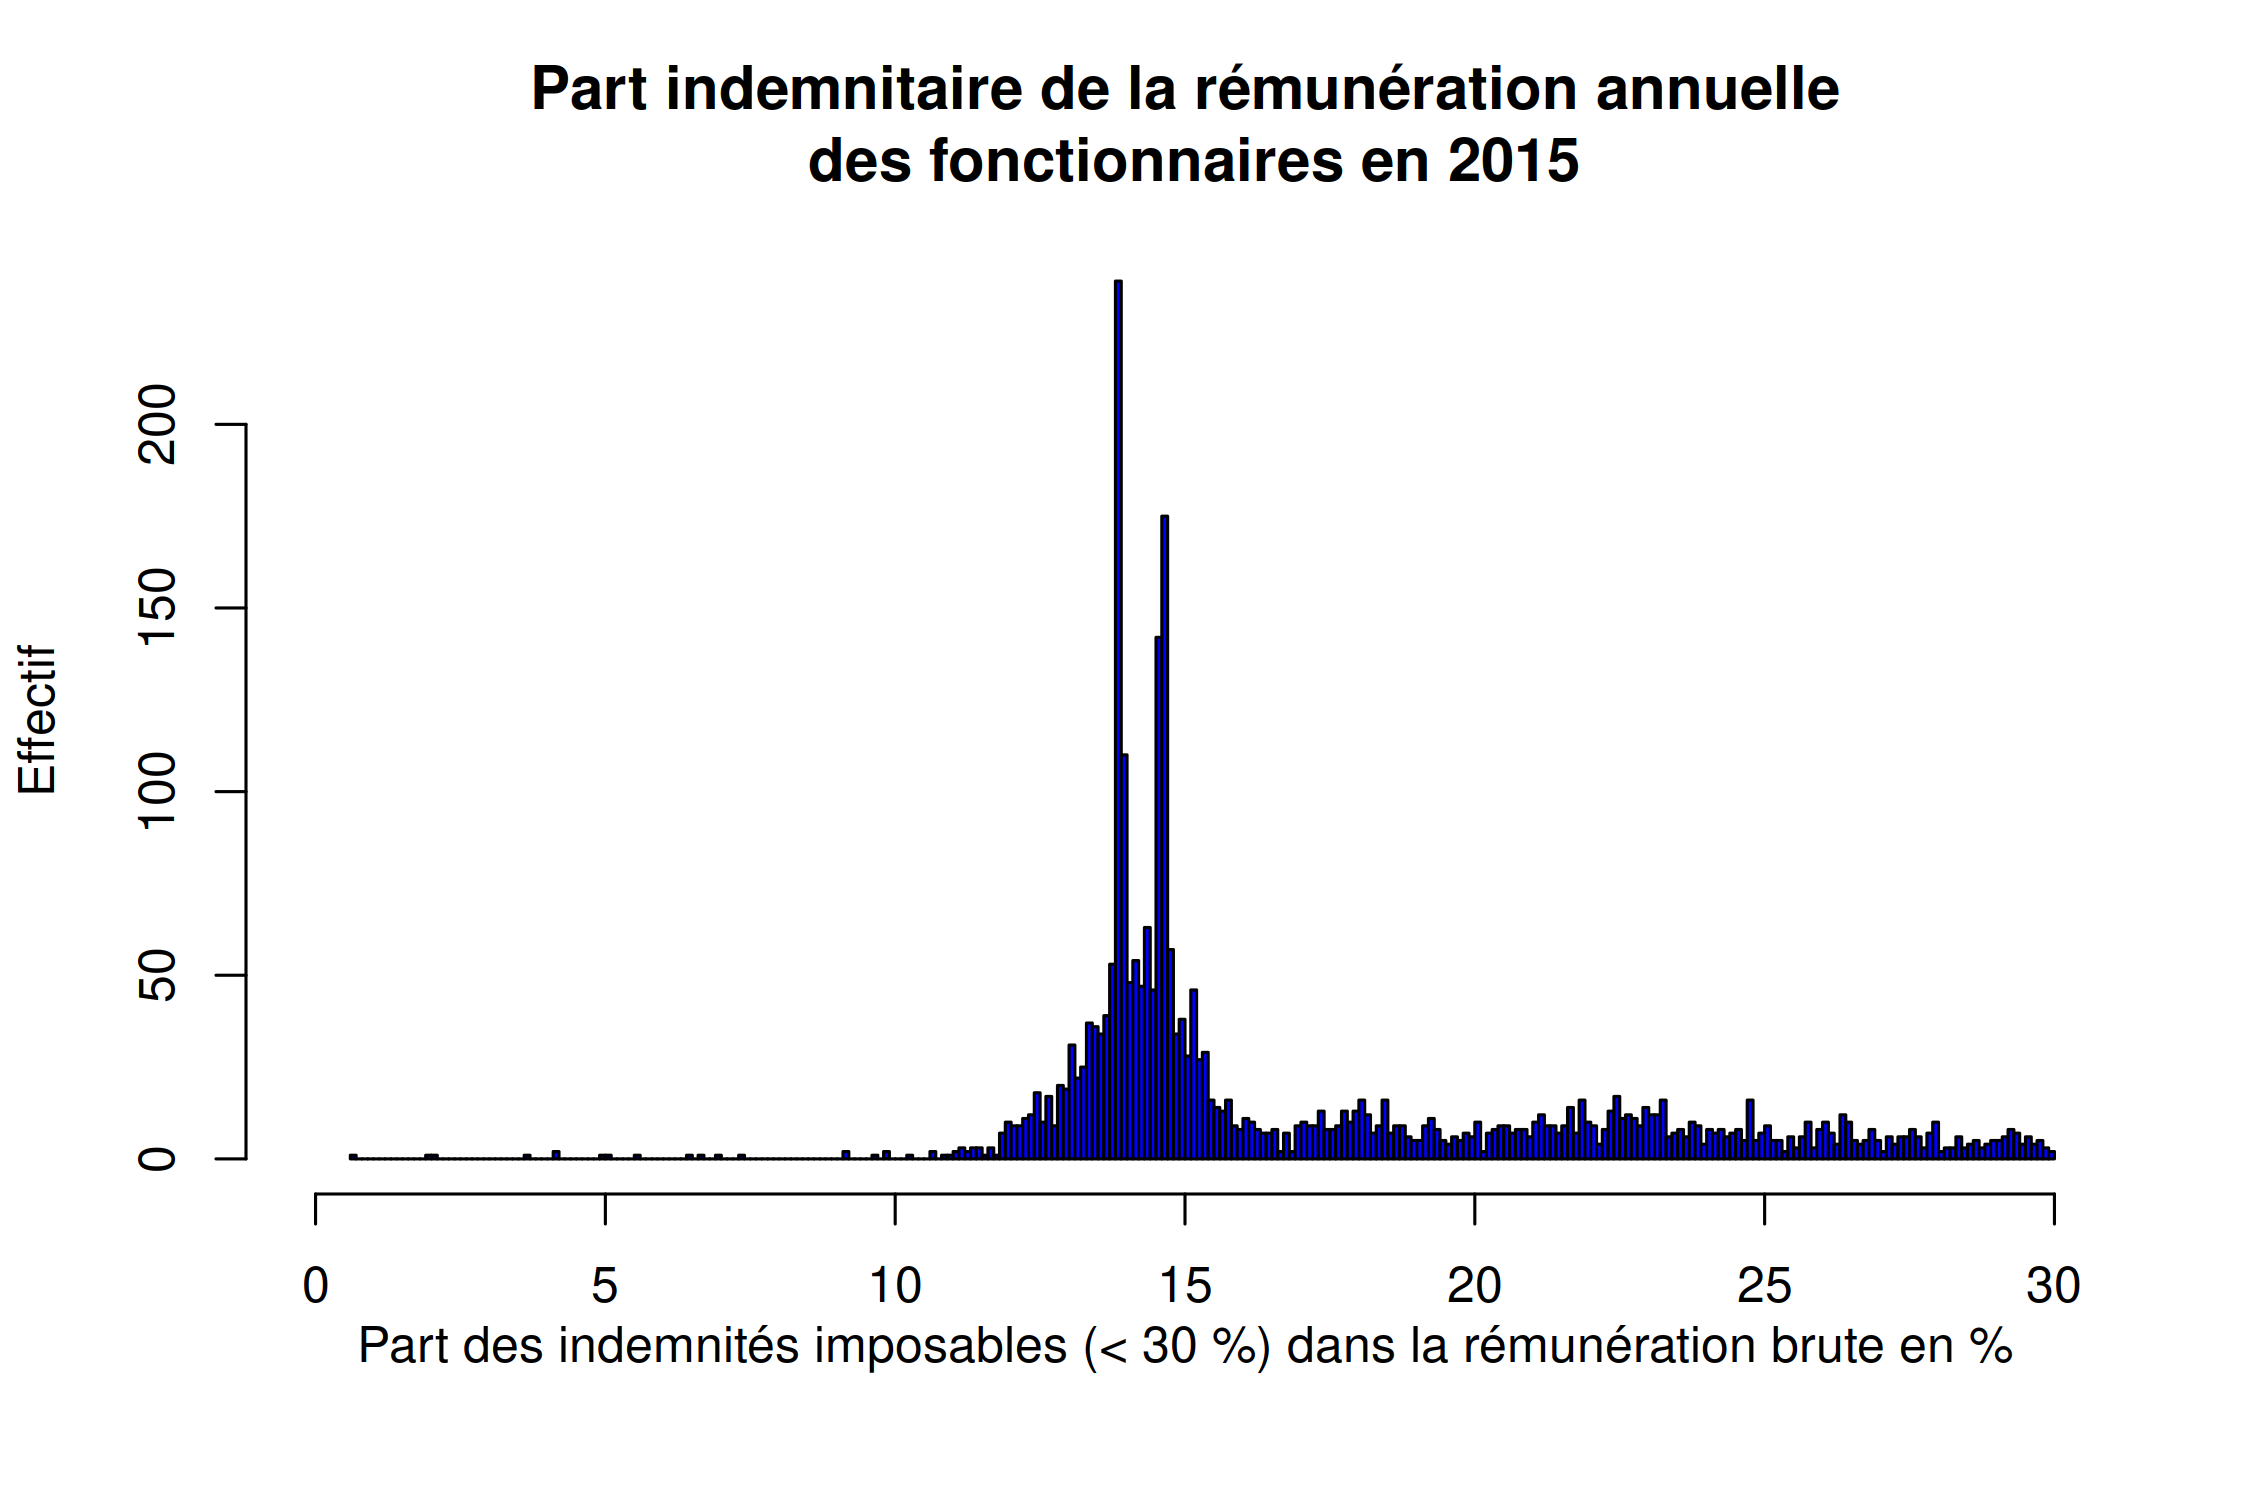
\includegraphics{altair_files/figure-latex/unnamed-chunk-43-5.png}

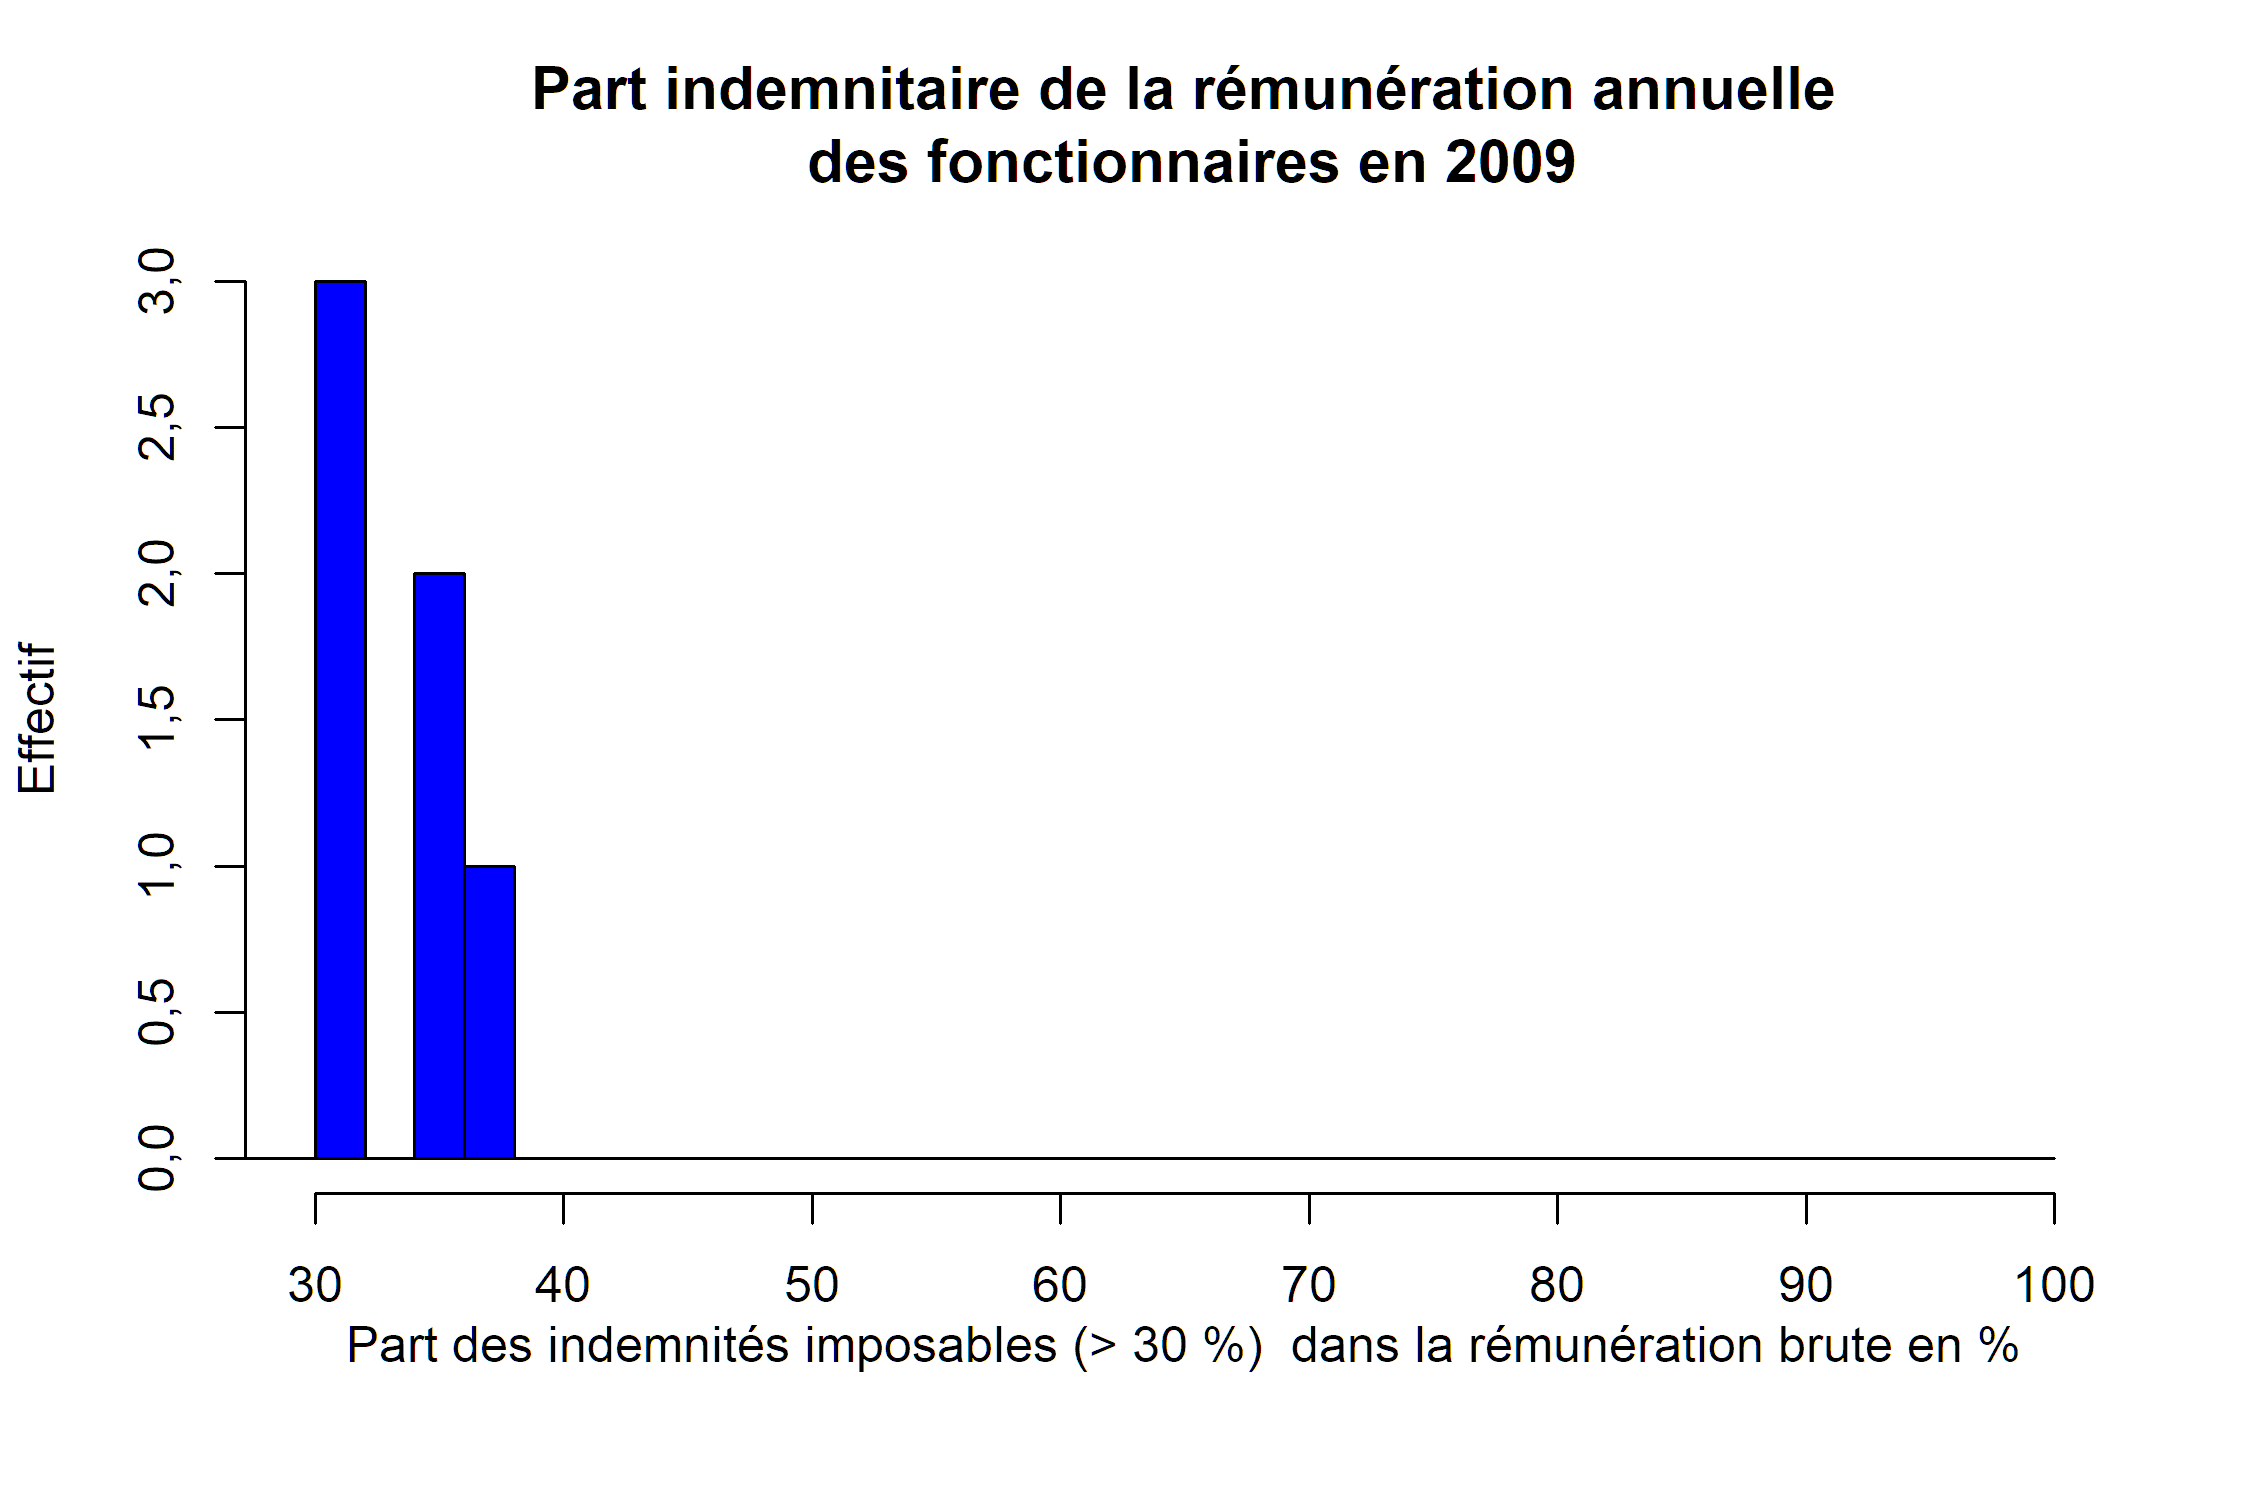
\includegraphics{altair_files/figure-latex/unnamed-chunk-43-6.png}

\textbf{Nota :}\\
\emph{Cet histogramme décrit l'évolution de la rémunération moyenne des
personnes en place (RMPP), définies comme présentes deux annees entières
consécutives avec la même quotité}\\
\emph{L'évolution de la RMPP permet d'étudier le glissement
vieillesse-technicité ``positif'', à effectifs constants sur deux
années}

\textbf{Effectif : 651 }

\textbf{Tests de cohérence}

Somme des rémunérations brutes versées aux personnels titulaires et
stagiaires :

~\emph{Tableau 2.2.1}

\begin{longtable}[]{@{}ll@{}}
\toprule
Agrégats & k€\tabularnewline
\midrule
\endhead
Brut annuel (bulletins) & 16 503 970,4\tabularnewline
Brut annuel (lignes) : & 16 635 201,7\tabularnewline
~dont ~~primes : & 2 272 122,6\tabularnewline
~dont ~autres rémunérations : &\tabularnewline
Part de primes en \% & 13,8\tabularnewline
\bottomrule
\end{longtable}

\textbf{Définitions :}

\emph{Brut annuel (bulletins)} : somme du champ \emph{Brut}\\
\emph{Brut annuel (lignes)} : somme du champ \emph{Montant} des lignes
de paye, dont :\\
\emph{Primes} : indemnités sauf remboursements, certaines IJSS,
Supplément familial de traitement et Indemnité de résidence\\
\emph{Autres rémunérations} : acomptes, retenues sur brut, rémunérations
diverses, rappels

\textbf{Tests de cohérence}

Somme des rémunérations brutes versées aux personnels (fonctionnaires) :

~\emph{Tableau 2.2.2}

\begin{longtable}[]{@{}ll@{}}
\toprule
Agrégats & k€\tabularnewline
\midrule
\endhead
Bulletins de paie & 16 503 970,4\tabularnewline
Lignes de paie & 16 635 201,7\tabularnewline
Difference & -131 231,3\tabularnewline
\bottomrule
\end{longtable}

A comparer aux soldes des comptes 6411, 6419 et 648 du compte de
gestion.

\textbf{Formation et distribution du salaire brut moyen par tête (SMPT)
en EQTP pour l'annee 2011 }

~\emph{Tableau 2.2.3}

\begin{longtable}[]{@{}rrrrrr@{}}
\toprule
\begin{minipage}[b]{0.14\columnwidth}\raggedleft
Statistique\strut
\end{minipage} & \begin{minipage}[b]{0.23\columnwidth}\raggedleft
Traitement indiciaire\strut
\end{minipage} & \begin{minipage}[b]{0.07\columnwidth}\raggedleft
Primes\strut
\end{minipage} & \begin{minipage}[b]{0.22\columnwidth}\raggedleft
Autres rémunérations\strut
\end{minipage} & \begin{minipage}[b]{0.08\columnwidth}\raggedleft
Quotité\strut
\end{minipage} & \begin{minipage}[b]{0.09\columnwidth}\raggedleft
Effectif\strut
\end{minipage}\tabularnewline
\midrule
\endhead
\begin{minipage}[t]{0.14\columnwidth}\raggedleft
Minimum\strut
\end{minipage} & \begin{minipage}[t]{0.23\columnwidth}\raggedleft
4 383\strut
\end{minipage} & \begin{minipage}[t]{0.07\columnwidth}\raggedleft
822\strut
\end{minipage} & \begin{minipage}[t]{0.22\columnwidth}\raggedleft
0\strut
\end{minipage} & \begin{minipage}[t]{0.08\columnwidth}\raggedleft
0,29\strut
\end{minipage} & \begin{minipage}[t]{0.09\columnwidth}\raggedleft
\strut
\end{minipage}\tabularnewline
\begin{minipage}[t]{0.14\columnwidth}\raggedleft
1er quartile\strut
\end{minipage} & \begin{minipage}[t]{0.23\columnwidth}\raggedleft
16 669\strut
\end{minipage} & \begin{minipage}[t]{0.07\columnwidth}\raggedleft
2 791\strut
\end{minipage} & \begin{minipage}[t]{0.22\columnwidth}\raggedleft
0\strut
\end{minipage} & \begin{minipage}[t]{0.08\columnwidth}\raggedleft
0,83\strut
\end{minipage} & \begin{minipage}[t]{0.09\columnwidth}\raggedleft
\strut
\end{minipage}\tabularnewline
\begin{minipage}[t]{0.14\columnwidth}\raggedleft
Médiane\strut
\end{minipage} & \begin{minipage}[t]{0.23\columnwidth}\raggedleft
19 724\strut
\end{minipage} & \begin{minipage}[t]{0.07\columnwidth}\raggedleft
3 574\strut
\end{minipage} & \begin{minipage}[t]{0.22\columnwidth}\raggedleft
0\strut
\end{minipage} & \begin{minipage}[t]{0.08\columnwidth}\raggedleft
1\strut
\end{minipage} & \begin{minipage}[t]{0.09\columnwidth}\raggedleft
\strut
\end{minipage}\tabularnewline
\begin{minipage}[t]{0.14\columnwidth}\raggedleft
Moyenne\strut
\end{minipage} & \begin{minipage}[t]{0.23\columnwidth}\raggedleft
20 835\strut
\end{minipage} & \begin{minipage}[t]{0.07\columnwidth}\raggedleft
3 746\strut
\end{minipage} & \begin{minipage}[t]{0.22\columnwidth}\raggedleft
0\strut
\end{minipage} & \begin{minipage}[t]{0.08\columnwidth}\raggedleft
0,93\strut
\end{minipage} & \begin{minipage}[t]{0.09\columnwidth}\raggedleft
614\strut
\end{minipage}\tabularnewline
\begin{minipage}[t]{0.14\columnwidth}\raggedleft
3ème quartile\strut
\end{minipage} & \begin{minipage}[t]{0.23\columnwidth}\raggedleft
23 464\strut
\end{minipage} & \begin{minipage}[t]{0.07\columnwidth}\raggedleft
4 365\strut
\end{minipage} & \begin{minipage}[t]{0.22\columnwidth}\raggedleft
0\strut
\end{minipage} & \begin{minipage}[t]{0.08\columnwidth}\raggedleft
1\strut
\end{minipage} & \begin{minipage}[t]{0.09\columnwidth}\raggedleft
\strut
\end{minipage}\tabularnewline
\begin{minipage}[t]{0.14\columnwidth}\raggedleft
Maximum\strut
\end{minipage} & \begin{minipage}[t]{0.23\columnwidth}\raggedleft
58 786\strut
\end{minipage} & \begin{minipage}[t]{0.07\columnwidth}\raggedleft
26 704\strut
\end{minipage} & \begin{minipage}[t]{0.22\columnwidth}\raggedleft
0\strut
\end{minipage} & \begin{minipage}[t]{0.08\columnwidth}\raggedleft
1\strut
\end{minipage} & \begin{minipage}[t]{0.09\columnwidth}\raggedleft
\strut
\end{minipage}\tabularnewline
\bottomrule
\end{longtable}

~\emph{Tableau 2.2.4}

\begin{longtable}[]{@{}rrrrrrr@{}}
\toprule
\begin{minipage}[b]{0.11\columnwidth}\raggedleft
Statistique\strut
\end{minipage} & \begin{minipage}[b]{0.20\columnwidth}\raggedleft
Total lignes hors rappels\strut
\end{minipage} & \begin{minipage}[b]{0.09\columnwidth}\raggedleft
Total brut\strut
\end{minipage} & \begin{minipage}[b]{0.14\columnwidth}\raggedleft
SMPT brut en EQTP\strut
\end{minipage} & \begin{minipage}[b]{0.14\columnwidth}\raggedleft
Part indemnitaire\strut
\end{minipage} & \begin{minipage}[b]{0.06\columnwidth}\raggedleft
Quotité\strut
\end{minipage} & \begin{minipage}[b]{0.07\columnwidth}\raggedleft
Effectif\strut
\end{minipage}\tabularnewline
\midrule
\endhead
\begin{minipage}[t]{0.11\columnwidth}\raggedleft
Minimum\strut
\end{minipage} & \begin{minipage}[t]{0.20\columnwidth}\raggedleft
8 044\strut
\end{minipage} & \begin{minipage}[t]{0.09\columnwidth}\raggedleft
8 030\strut
\end{minipage} & \begin{minipage}[t]{0.14\columnwidth}\raggedleft
121 906\strut
\end{minipage} & \begin{minipage}[t]{0.14\columnwidth}\raggedleft
6\strut
\end{minipage} & \begin{minipage}[t]{0.06\columnwidth}\raggedleft
0,29\strut
\end{minipage} & \begin{minipage}[t]{0.07\columnwidth}\raggedleft
\strut
\end{minipage}\tabularnewline
\begin{minipage}[t]{0.11\columnwidth}\raggedleft
1er quartile\strut
\end{minipage} & \begin{minipage}[t]{0.20\columnwidth}\raggedleft
22 186\strut
\end{minipage} & \begin{minipage}[t]{0.09\columnwidth}\raggedleft
22 074\strut
\end{minipage} & \begin{minipage}[t]{0.14\columnwidth}\raggedleft
278 596\strut
\end{minipage} & \begin{minipage}[t]{0.14\columnwidth}\raggedleft
10\strut
\end{minipage} & \begin{minipage}[t]{0.06\columnwidth}\raggedleft
0,83\strut
\end{minipage} & \begin{minipage}[t]{0.07\columnwidth}\raggedleft
\strut
\end{minipage}\tabularnewline
\begin{minipage}[t]{0.11\columnwidth}\raggedleft
Médiane\strut
\end{minipage} & \begin{minipage}[t]{0.20\columnwidth}\raggedleft
25 725\strut
\end{minipage} & \begin{minipage}[t]{0.09\columnwidth}\raggedleft
25 745\strut
\end{minipage} & \begin{minipage}[t]{0.14\columnwidth}\raggedleft
320 005\strut
\end{minipage} & \begin{minipage}[t]{0.14\columnwidth}\raggedleft
14\strut
\end{minipage} & \begin{minipage}[t]{0.06\columnwidth}\raggedleft
1\strut
\end{minipage} & \begin{minipage}[t]{0.07\columnwidth}\raggedleft
\strut
\end{minipage}\tabularnewline
\begin{minipage}[t]{0.11\columnwidth}\raggedleft
Moyenne\strut
\end{minipage} & \begin{minipage}[t]{0.20\columnwidth}\raggedleft
27 601\strut
\end{minipage} & \begin{minipage}[t]{0.09\columnwidth}\raggedleft
27 389\strut
\end{minipage} & \begin{minipage}[t]{0.14\columnwidth}\raggedleft
343 408\strut
\end{minipage} & \begin{minipage}[t]{0.14\columnwidth}\raggedleft
14\strut
\end{minipage} & \begin{minipage}[t]{0.06\columnwidth}\raggedleft
0,93\strut
\end{minipage} & \begin{minipage}[t]{0.07\columnwidth}\raggedleft
614\strut
\end{minipage}\tabularnewline
\begin{minipage}[t]{0.11\columnwidth}\raggedleft
3ème quartile\strut
\end{minipage} & \begin{minipage}[t]{0.20\columnwidth}\raggedleft
30 984\strut
\end{minipage} & \begin{minipage}[t]{0.09\columnwidth}\raggedleft
30 910\strut
\end{minipage} & \begin{minipage}[t]{0.14\columnwidth}\raggedleft
395 085\strut
\end{minipage} & \begin{minipage}[t]{0.14\columnwidth}\raggedleft
16\strut
\end{minipage} & \begin{minipage}[t]{0.06\columnwidth}\raggedleft
1\strut
\end{minipage} & \begin{minipage}[t]{0.07\columnwidth}\raggedleft
\strut
\end{minipage}\tabularnewline
\begin{minipage}[t]{0.11\columnwidth}\raggedleft
Maximum\strut
\end{minipage} & \begin{minipage}[t]{0.20\columnwidth}\raggedleft
103 687\strut
\end{minipage} & \begin{minipage}[t]{0.09\columnwidth}\raggedleft
102 643\strut
\end{minipage} & \begin{minipage}[t]{0.14\columnwidth}\raggedleft
1 208 537\strut
\end{minipage} & \begin{minipage}[t]{0.14\columnwidth}\raggedleft
51\strut
\end{minipage} & \begin{minipage}[t]{0.06\columnwidth}\raggedleft
1\strut
\end{minipage} & \begin{minipage}[t]{0.07\columnwidth}\raggedleft
\strut
\end{minipage}\tabularnewline
\bottomrule
\end{longtable}

\emph{Hors vacataires identifiés, assistantes maternelles, élus locaux
et pour les postes actifs non annexes}

\textbf{Categorie A}

~\emph{Tableau 2.2.5}

\begin{longtable}[]{@{}rrrrr@{}}
\toprule
Statistique & Traitement indiciaire & Primes & Autres rémunérations &
Quotité\tabularnewline
\midrule
\endhead
Minimum & 8 524 & 1 175 & 0 & 0,33\tabularnewline
1er quartile & 20 614 & 3 184 & 0 & 0,8\tabularnewline
Médiane & 25 232 & 3 818 & 0 & 1\tabularnewline
Moyenne & 25 136 & 4 430 & 0 & 0,91\tabularnewline
3ème quartile & 28 912 & 5 024 & 0 & 1\tabularnewline
Maximum & 58 786 & 26 704 & 0 & 1\tabularnewline
\bottomrule
\end{longtable}

~\emph{Tableau 2.2.6}

\begin{longtable}[]{@{}rrrrr@{}}
\toprule
\begin{minipage}[b]{0.14\columnwidth}\raggedleft
Statistique\strut
\end{minipage} & \begin{minipage}[b]{0.20\columnwidth}\raggedleft
Total rémunérations\strut
\end{minipage} & \begin{minipage}[b]{0.25\columnwidth}\raggedleft
Total rémunérations EQTP\strut
\end{minipage} & \begin{minipage}[b]{0.18\columnwidth}\raggedleft
Part indemnitaire\strut
\end{minipage} & \begin{minipage}[b]{0.08\columnwidth}\raggedleft
Quotité\strut
\end{minipage}\tabularnewline
\midrule
\endhead
\begin{minipage}[t]{0.14\columnwidth}\raggedleft
Minimum\strut
\end{minipage} & \begin{minipage}[t]{0.20\columnwidth}\raggedleft
11 057\strut
\end{minipage} & \begin{minipage}[t]{0.25\columnwidth}\raggedleft
132 155\strut
\end{minipage} & \begin{minipage}[t]{0.18\columnwidth}\raggedleft
8,4\strut
\end{minipage} & \begin{minipage}[t]{0.08\columnwidth}\raggedleft
0,33\strut
\end{minipage}\tabularnewline
\begin{minipage}[t]{0.14\columnwidth}\raggedleft
1er quartile\strut
\end{minipage} & \begin{minipage}[t]{0.20\columnwidth}\raggedleft
26 577\strut
\end{minipage} & \begin{minipage}[t]{0.25\columnwidth}\raggedleft
362 360\strut
\end{minipage} & \begin{minipage}[t]{0.18\columnwidth}\raggedleft
11\strut
\end{minipage} & \begin{minipage}[t]{0.08\columnwidth}\raggedleft
0,8\strut
\end{minipage}\tabularnewline
\begin{minipage}[t]{0.14\columnwidth}\raggedleft
Médiane\strut
\end{minipage} & \begin{minipage}[t]{0.20\columnwidth}\raggedleft
32 244\strut
\end{minipage} & \begin{minipage}[t]{0.25\columnwidth}\raggedleft
414 768\strut
\end{minipage} & \begin{minipage}[t]{0.18\columnwidth}\raggedleft
12\strut
\end{minipage} & \begin{minipage}[t]{0.08\columnwidth}\raggedleft
1\strut
\end{minipage}\tabularnewline
\begin{minipage}[t]{0.14\columnwidth}\raggedleft
Moyenne\strut
\end{minipage} & \begin{minipage}[t]{0.20\columnwidth}\raggedleft
33 059\strut
\end{minipage} & \begin{minipage}[t]{0.25\columnwidth}\raggedleft
421 901\strut
\end{minipage} & \begin{minipage}[t]{0.18\columnwidth}\raggedleft
13\strut
\end{minipage} & \begin{minipage}[t]{0.08\columnwidth}\raggedleft
0,91\strut
\end{minipage}\tabularnewline
\begin{minipage}[t]{0.14\columnwidth}\raggedleft
3ème quartile\strut
\end{minipage} & \begin{minipage}[t]{0.20\columnwidth}\raggedleft
37 338\strut
\end{minipage} & \begin{minipage}[t]{0.25\columnwidth}\raggedleft
472 262\strut
\end{minipage} & \begin{minipage}[t]{0.18\columnwidth}\raggedleft
14\strut
\end{minipage} & \begin{minipage}[t]{0.08\columnwidth}\raggedleft
1\strut
\end{minipage}\tabularnewline
\begin{minipage}[t]{0.14\columnwidth}\raggedleft
Maximum\strut
\end{minipage} & \begin{minipage}[t]{0.20\columnwidth}\raggedleft
102 643\strut
\end{minipage} & \begin{minipage}[t]{0.25\columnwidth}\raggedleft
1 208 537\strut
\end{minipage} & \begin{minipage}[t]{0.18\columnwidth}\raggedleft
35\strut
\end{minipage} & \begin{minipage}[t]{0.08\columnwidth}\raggedleft
1\strut
\end{minipage}\tabularnewline
\bottomrule
\end{longtable}

\textbf{Effectif : 226 }

\textbf{Categorie B}

~\emph{Tableau 2.2.7}

\begin{longtable}[]{@{}rrrrr@{}}
\toprule
Statistique & Traitement indiciaire & Primes & Autres rémunérations &
Quotité\tabularnewline
\midrule
\endhead
Minimum & 13 942 & 1 711 & 0 & 0,65\tabularnewline
1er quartile & 20 447 & 3 141 & 0 & 0,9\tabularnewline
Médiane & 23 466 & 3 288 & 0 & 1\tabularnewline
Moyenne & 23 846 & 4 027 & 0 & 0,94\tabularnewline
3ème quartile & 28 825 & 4 542 & 0 & 1\tabularnewline
Maximum & 29 986 & 12 938 & 0 & 1\tabularnewline
\bottomrule
\end{longtable}

~\emph{Tableau 2.2.8}

\begin{longtable}[]{@{}rrrrr@{}}
\toprule
\begin{minipage}[b]{0.12\columnwidth}\raggedleft
Statistique\strut
\end{minipage} & \begin{minipage}[b]{0.17\columnwidth}\raggedleft
Total rémunérations\strut
\end{minipage} & \begin{minipage}[b]{0.21\columnwidth}\raggedleft
Total rémunérations EQTP\strut
\end{minipage} & \begin{minipage}[b]{0.31\columnwidth}\raggedleft
Part de la rémunération indemnitaire\strut
\end{minipage} & \begin{minipage}[b]{0.07\columnwidth}\raggedleft
Quotité\strut
\end{minipage}\tabularnewline
\midrule
\endhead
\begin{minipage}[t]{0.12\columnwidth}\raggedleft
Minimum\strut
\end{minipage} & \begin{minipage}[t]{0.17\columnwidth}\raggedleft
17 535\strut
\end{minipage} & \begin{minipage}[t]{0.21\columnwidth}\raggedleft
241 678\strut
\end{minipage} & \begin{minipage}[t]{0.31\columnwidth}\raggedleft
7,1\strut
\end{minipage} & \begin{minipage}[t]{0.07\columnwidth}\raggedleft
0,65\strut
\end{minipage}\tabularnewline
\begin{minipage}[t]{0.12\columnwidth}\raggedleft
1er quartile\strut
\end{minipage} & \begin{minipage}[t]{0.17\columnwidth}\raggedleft
25 382\strut
\end{minipage} & \begin{minipage}[t]{0.21\columnwidth}\raggedleft
337 183\strut
\end{minipage} & \begin{minipage}[t]{0.31\columnwidth}\raggedleft
9,4\strut
\end{minipage} & \begin{minipage}[t]{0.07\columnwidth}\raggedleft
0,9\strut
\end{minipage}\tabularnewline
\begin{minipage}[t]{0.12\columnwidth}\raggedleft
Médiane\strut
\end{minipage} & \begin{minipage}[t]{0.17\columnwidth}\raggedleft
30 856\strut
\end{minipage} & \begin{minipage}[t]{0.21\columnwidth}\raggedleft
379 795\strut
\end{minipage} & \begin{minipage}[t]{0.31\columnwidth}\raggedleft
11\strut
\end{minipage} & \begin{minipage}[t]{0.07\columnwidth}\raggedleft
1\strut
\end{minipage}\tabularnewline
\begin{minipage}[t]{0.12\columnwidth}\raggedleft
Moyenne\strut
\end{minipage} & \begin{minipage}[t]{0.17\columnwidth}\raggedleft
30 362\strut
\end{minipage} & \begin{minipage}[t]{0.21\columnwidth}\raggedleft
377 561\strut
\end{minipage} & \begin{minipage}[t]{0.31\columnwidth}\raggedleft
13\strut
\end{minipage} & \begin{minipage}[t]{0.07\columnwidth}\raggedleft
0,94\strut
\end{minipage}\tabularnewline
\begin{minipage}[t]{0.12\columnwidth}\raggedleft
3ème quartile\strut
\end{minipage} & \begin{minipage}[t]{0.17\columnwidth}\raggedleft
35 804\strut
\end{minipage} & \begin{minipage}[t]{0.21\columnwidth}\raggedleft
442 584\strut
\end{minipage} & \begin{minipage}[t]{0.31\columnwidth}\raggedleft
15\strut
\end{minipage} & \begin{minipage}[t]{0.07\columnwidth}\raggedleft
1\strut
\end{minipage}\tabularnewline
\begin{minipage}[t]{0.12\columnwidth}\raggedleft
Maximum\strut
\end{minipage} & \begin{minipage}[t]{0.17\columnwidth}\raggedleft
43 372\strut
\end{minipage} & \begin{minipage}[t]{0.21\columnwidth}\raggedleft
510 669\strut
\end{minipage} & \begin{minipage}[t]{0.31\columnwidth}\raggedleft
30\strut
\end{minipage} & \begin{minipage}[t]{0.07\columnwidth}\raggedleft
1\strut
\end{minipage}\tabularnewline
\bottomrule
\end{longtable}

\textbf{Effectif : 43 }

\textbf{Categorie C}

~\emph{Tableau 2.2.9}

\begin{longtable}[]{@{}rrrrr@{}}
\toprule
Statistique & Traitement indiciaire & Primes & Autres rémunérations &
Quotité\tabularnewline
\midrule
\endhead
Minimum & 4 515 & 822 & 0 & 0,38\tabularnewline
1er quartile & 16 544 & 2 081 & 0 & 0,95\tabularnewline
Médiane & 17 015 & 3 572 & 0 & 1\tabularnewline
Moyenne & 17 549 & 3 321 & 0 & 0,95\tabularnewline
3ème quartile & 19 447 & 4 202 & 0 & 1\tabularnewline
Maximum & 23 892 & 7 849 & 0 & 1\tabularnewline
\bottomrule
\end{longtable}

~\emph{Tableau 2.2.10}

\begin{longtable}[]{@{}rrrrr@{}}
\toprule
\begin{minipage}[b]{0.12\columnwidth}\raggedleft
Statistique\strut
\end{minipage} & \begin{minipage}[b]{0.17\columnwidth}\raggedleft
Total rémunérations\strut
\end{minipage} & \begin{minipage}[b]{0.21\columnwidth}\raggedleft
Total rémunérations EQTP\strut
\end{minipage} & \begin{minipage}[b]{0.31\columnwidth}\raggedleft
Part de la rémunération indemnitaire\strut
\end{minipage} & \begin{minipage}[b]{0.07\columnwidth}\raggedleft
Quotité\strut
\end{minipage}\tabularnewline
\midrule
\endhead
\begin{minipage}[t]{0.12\columnwidth}\raggedleft
Minimum\strut
\end{minipage} & \begin{minipage}[t]{0.17\columnwidth}\raggedleft
8 660\strut
\end{minipage} & \begin{minipage}[t]{0.21\columnwidth}\raggedleft
153 148\strut
\end{minipage} & \begin{minipage}[t]{0.31\columnwidth}\raggedleft
6\strut
\end{minipage} & \begin{minipage}[t]{0.07\columnwidth}\raggedleft
0,38\strut
\end{minipage}\tabularnewline
\begin{minipage}[t]{0.12\columnwidth}\raggedleft
1er quartile\strut
\end{minipage} & \begin{minipage}[t]{0.17\columnwidth}\raggedleft
20 648\strut
\end{minipage} & \begin{minipage}[t]{0.21\columnwidth}\raggedleft
258 936\strut
\end{minipage} & \begin{minipage}[t]{0.31\columnwidth}\raggedleft
10\strut
\end{minipage} & \begin{minipage}[t]{0.07\columnwidth}\raggedleft
0,95\strut
\end{minipage}\tabularnewline
\begin{minipage}[t]{0.12\columnwidth}\raggedleft
Médiane\strut
\end{minipage} & \begin{minipage}[t]{0.17\columnwidth}\raggedleft
23 194\strut
\end{minipage} & \begin{minipage}[t]{0.21\columnwidth}\raggedleft
287 671\strut
\end{minipage} & \begin{minipage}[t]{0.31\columnwidth}\raggedleft
15\strut
\end{minipage} & \begin{minipage}[t]{0.07\columnwidth}\raggedleft
1\strut
\end{minipage}\tabularnewline
\begin{minipage}[t]{0.12\columnwidth}\raggedleft
Moyenne\strut
\end{minipage} & \begin{minipage}[t]{0.17\columnwidth}\raggedleft
23 305\strut
\end{minipage} & \begin{minipage}[t]{0.21\columnwidth}\raggedleft
288 104\strut
\end{minipage} & \begin{minipage}[t]{0.31\columnwidth}\raggedleft
14\strut
\end{minipage} & \begin{minipage}[t]{0.07\columnwidth}\raggedleft
0,95\strut
\end{minipage}\tabularnewline
\begin{minipage}[t]{0.12\columnwidth}\raggedleft
3ème quartile\strut
\end{minipage} & \begin{minipage}[t]{0.17\columnwidth}\raggedleft
25 875\strut
\end{minipage} & \begin{minipage}[t]{0.21\columnwidth}\raggedleft
318 245\strut
\end{minipage} & \begin{minipage}[t]{0.31\columnwidth}\raggedleft
17\strut
\end{minipage} & \begin{minipage}[t]{0.07\columnwidth}\raggedleft
1\strut
\end{minipage}\tabularnewline
\begin{minipage}[t]{0.12\columnwidth}\raggedleft
Maximum\strut
\end{minipage} & \begin{minipage}[t]{0.17\columnwidth}\raggedleft
32 697\strut
\end{minipage} & \begin{minipage}[t]{0.21\columnwidth}\raggedleft
423 014\strut
\end{minipage} & \begin{minipage}[t]{0.31\columnwidth}\raggedleft
51\strut
\end{minipage} & \begin{minipage}[t]{0.07\columnwidth}\raggedleft
1\strut
\end{minipage}\tabularnewline
\bottomrule
\end{longtable}

\textbf{Effectif : 326 }

\hypertarget{contractuels-vacataires-et-stagiaires-inclus}{%
\subsection{2.3 Contractuels, vacataires et stagiaires
inclus}\label{contractuels-vacataires-et-stagiaires-inclus}}

\emph{Les assistantes maternelles et les vacataires sont ici inclus,
pour les postes non annexes}

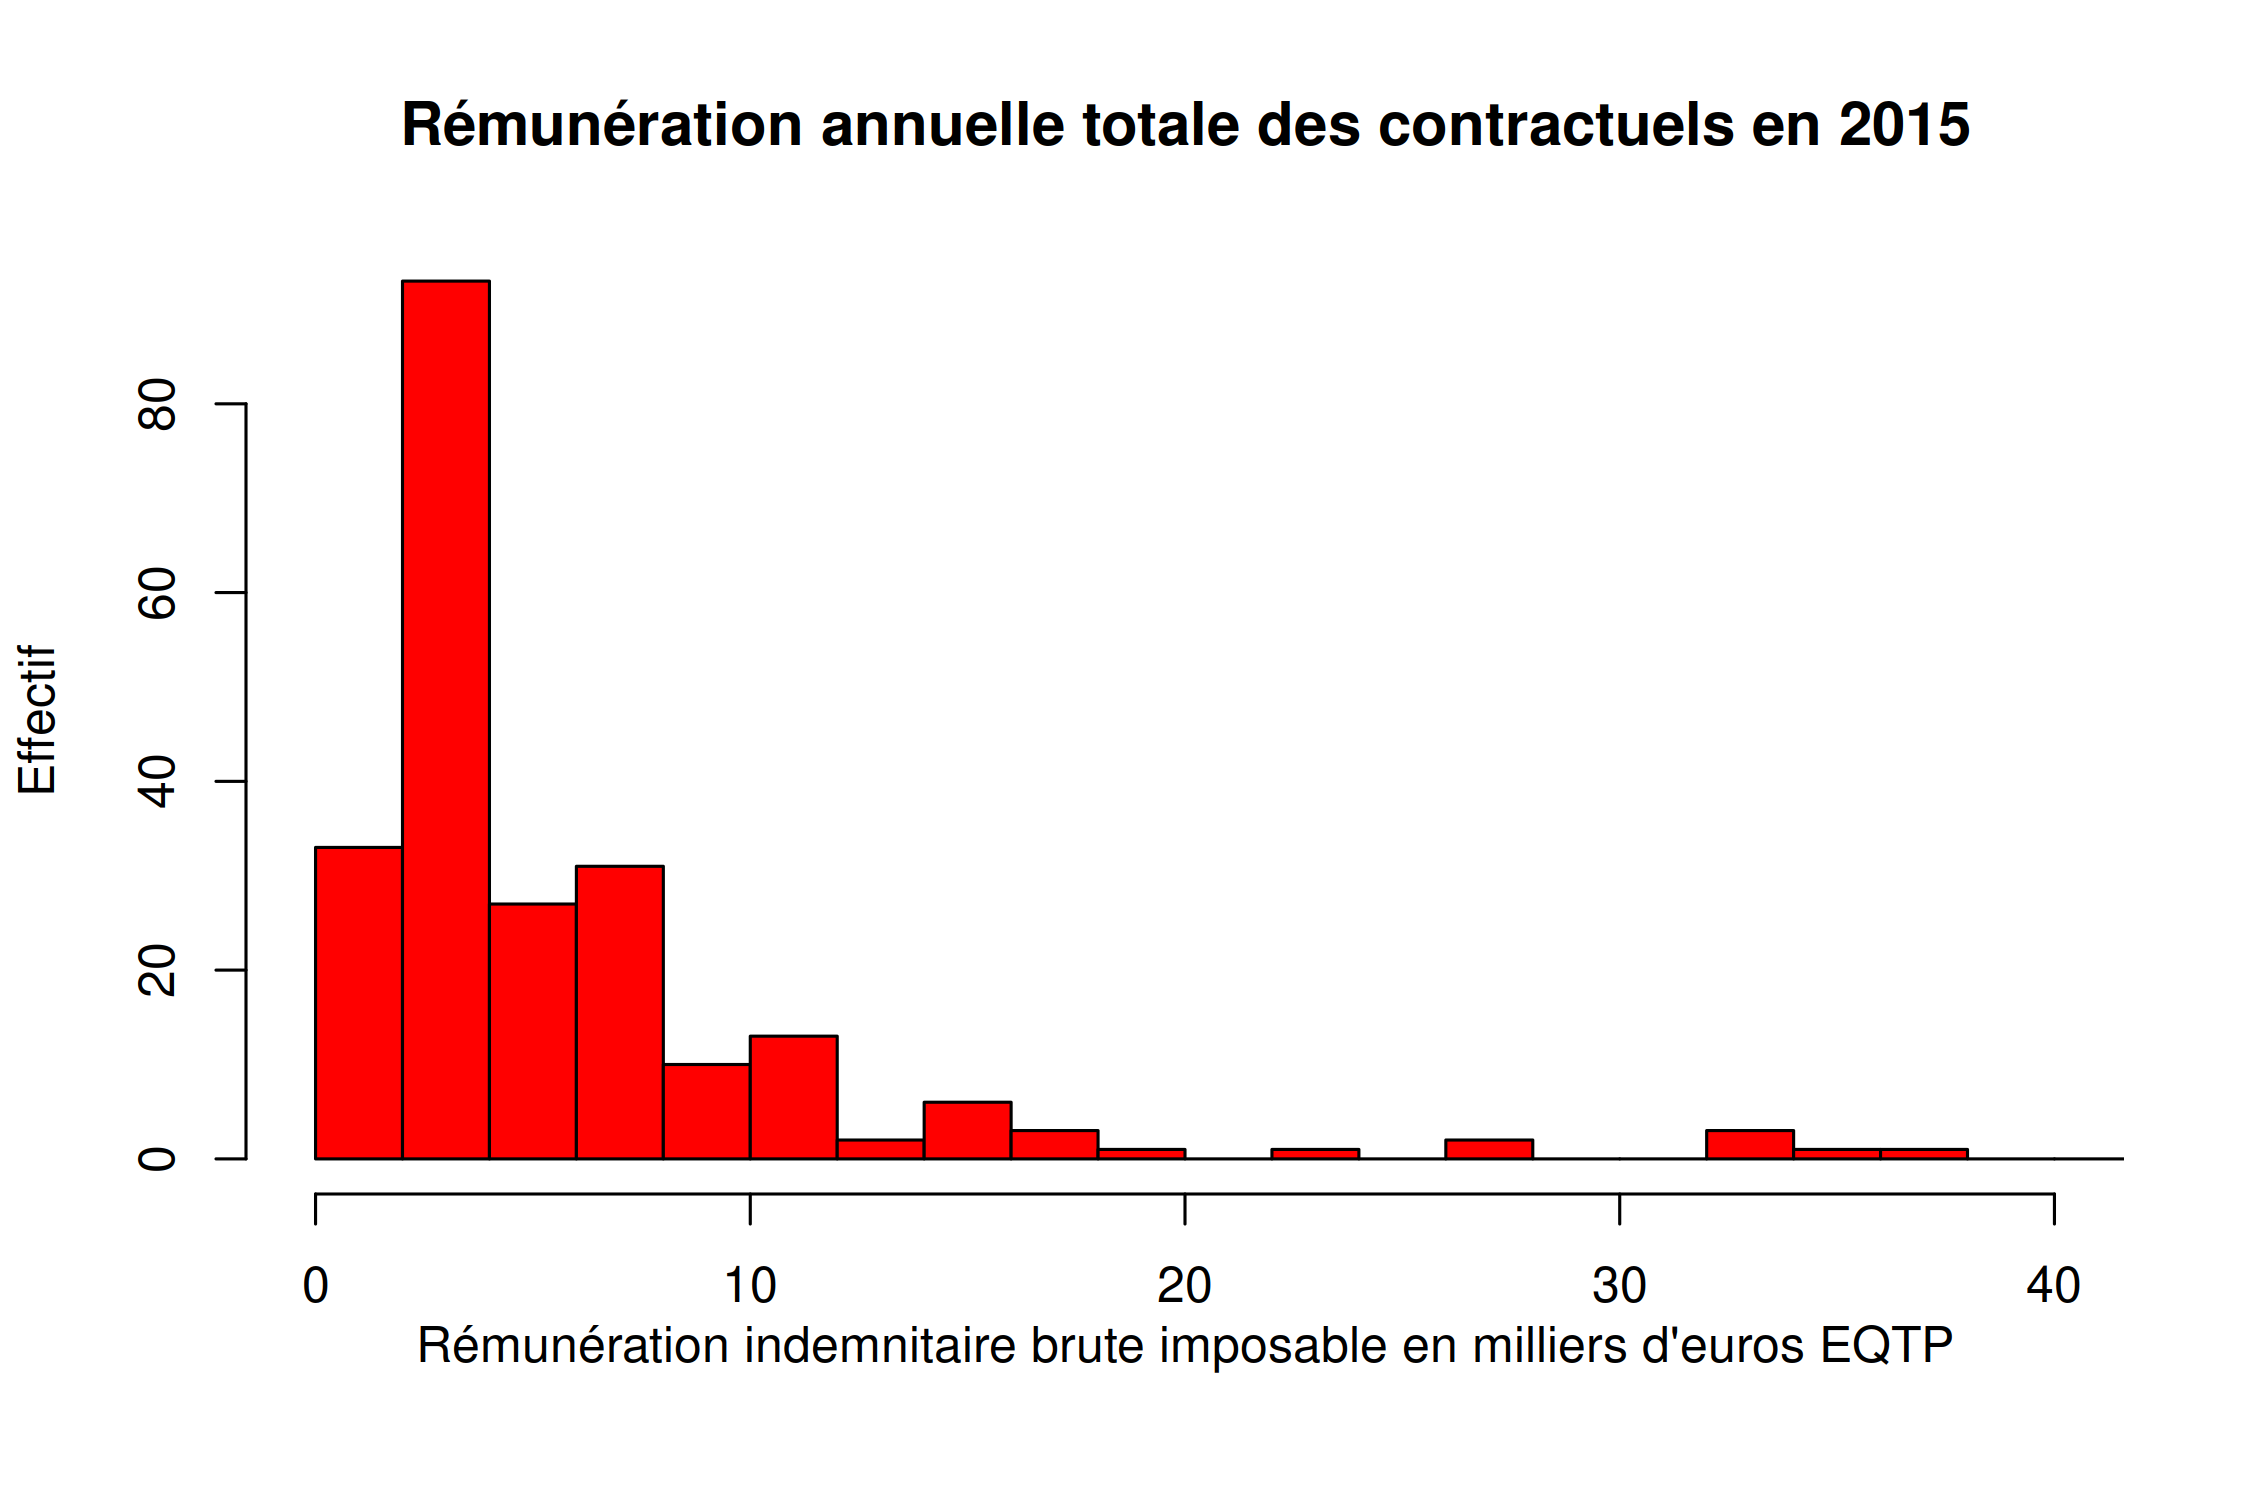
\includegraphics{altair_files/figure-latex/unnamed-chunk-61-1.png}

\textbf{Nota :} Ne sont retenues que les rémunérations supérieures à 1
000 k€. Les élus ne sont pas pris en compte.

\textbf{Formation et distribution du salaire brut moyen par tête (SMPT)
en EQTP pour l'année 2011 }

~\emph{Tableau 2.3.1}

\begin{longtable}[]{@{}rrrrr@{}}
\toprule
Statistique & Primes & Autres rémunérations & Quotité &
Effectif\tabularnewline
\midrule
\endhead
Minimum & -12 272 & 0 & 0,17 &\tabularnewline
1er quartile & 989 & 0 & 0,8 &\tabularnewline
Médiane & 1 601 & 0 & 1 &\tabularnewline
Moyenne & 2 255 & 0 & 0,87 & 308\tabularnewline
3ème quartile & 3 145 & 0 & 1 &\tabularnewline
Maximum & 21 403 & 0 & 1 &\tabularnewline
\bottomrule
\end{longtable}

~\emph{Tableau 2.3.2}

\begin{longtable}[]{@{}rrrrr@{}}
\toprule
Statistique & Total rémunérations & Total rémunérations EQTP & Quotité &
Effectif\tabularnewline
\midrule
\endhead
Minimum & 4 385 & 54 902 & 0,17 &\tabularnewline
1er quartile & 16 338 & 204 632 & 0,8 &\tabularnewline
Médiane & 19 326 & 237 907 & 1 &\tabularnewline
Moyenne & 31 676 & 385 103 & 0,87 & 308\tabularnewline
3ème quartile & 27 477 & 339 739 & 1 &\tabularnewline
Maximum & 128 668 & 1 514 960 & 1 &\tabularnewline
\bottomrule
\end{longtable}

\href{../Bases/Remunerations/Analyse.remunerations.csv}{Lien vers la base
des rémunérations}

\newpage

\hypertarget{remunerations-brutes-analyse-pour-le-dernier-exercice}{%
\section{3. Rémunérations brutes : analyse pour le dernier
exercice}\label{remunerations-brutes-analyse-pour-le-dernier-exercice}}

\textbf{Exercice : 2014 }

\hypertarget{remunerations-brutes-de-lensemble-des-agents-1}{%
\subsection{3.1 Rémunérations brutes de l'ensemble des
agents}\label{remunerations-brutes-de-lensemble-des-agents-1}}

\textbf{Cumuls des rémunérations brutes pour l'exercice 2014 }

\emph{Personnels (hors élus)}

~\emph{Tableau 3.1.1}

\begin{longtable}[]{@{}ll@{}}
\toprule
Agrégats & k€\tabularnewline
\midrule
\endhead
Brut annuel (bulletins) & 27 212 831,9\tabularnewline
Brut annuel (lignes) : & 27 185 653,3\tabularnewline
~dont ~Primes : & 3 089 288,8\tabularnewline
~dont ~Autres rémunérations &\tabularnewline
Part de primes en \% & 11,4\tabularnewline
\bottomrule
\end{longtable}

\textbf{Définitions :}

\emph{Brut annuel (bulletins)} : somme du champ \emph{Brut}\\
\emph{Brut annuel (lignes)} : somme du champ \emph{Montant} des lignes
de paye, dont :\\
\emph{Primes} : indemnités sauf remboursements, certaines IJSS,
indemnités d'élu le cas échéant, Supplément familial de traitement et
Indemnité de résidence\\
\emph{Autres rémunérations} : acomptes, retenues sur brut, rémunérations
diverses, rappels

\textbf{Tests de cohérence}

Somme des rémunérations brutes versées aux personnels (non élus) :

~\emph{Tableau 3.1.2}

\begin{longtable}[]{@{}ll@{}}
\toprule
Agrégats & k€\tabularnewline
\midrule
\endhead
Bulletins de paie & 27 212 831,9\tabularnewline
Lignes de paie & 27 185 653,3\tabularnewline
Difference & 27 178,6\tabularnewline
\bottomrule
\end{longtable}

à comparer aux soldes des comptes 641 et 648 du compte de gestion.

\hypertarget{remunerations-brutes-des-fonctionnaires-1}{%
\subsection{3.2 Rémunérations brutes des
fonctionnaires}\label{remunerations-brutes-des-fonctionnaires-1}}

\emph{Cette section concerne les personnels fonctionnaires titulaires et
stagiaires}

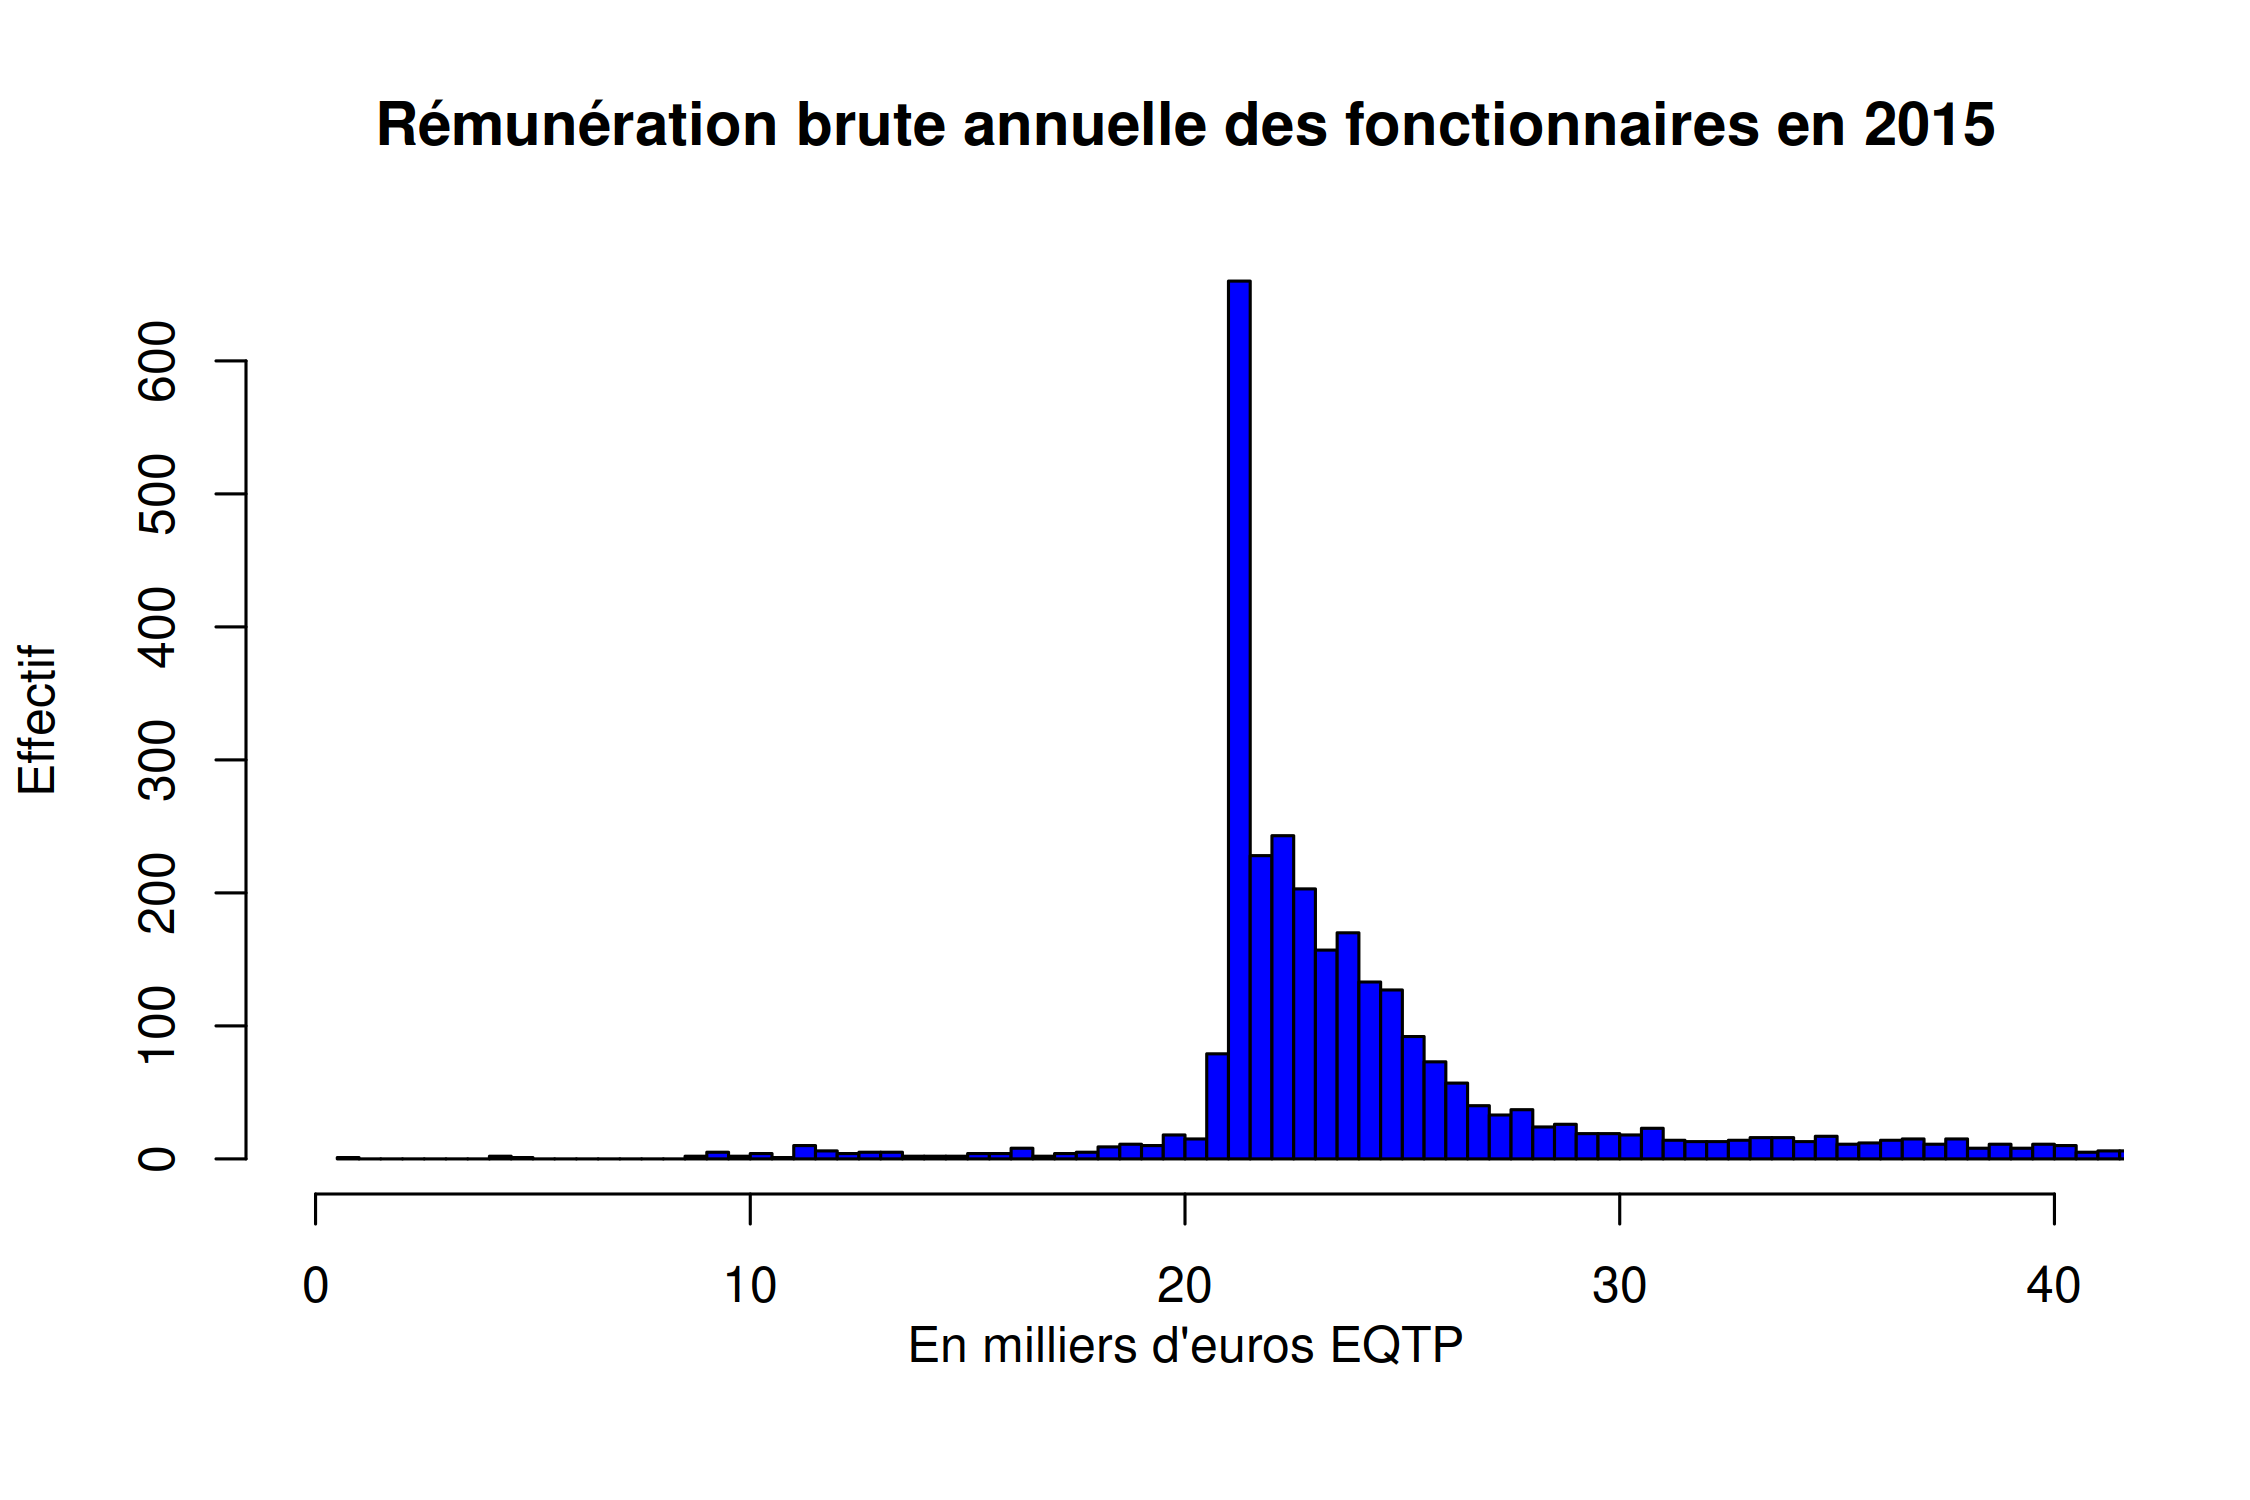
\includegraphics{altair_files/figure-latex/unnamed-chunk-76-1.png}

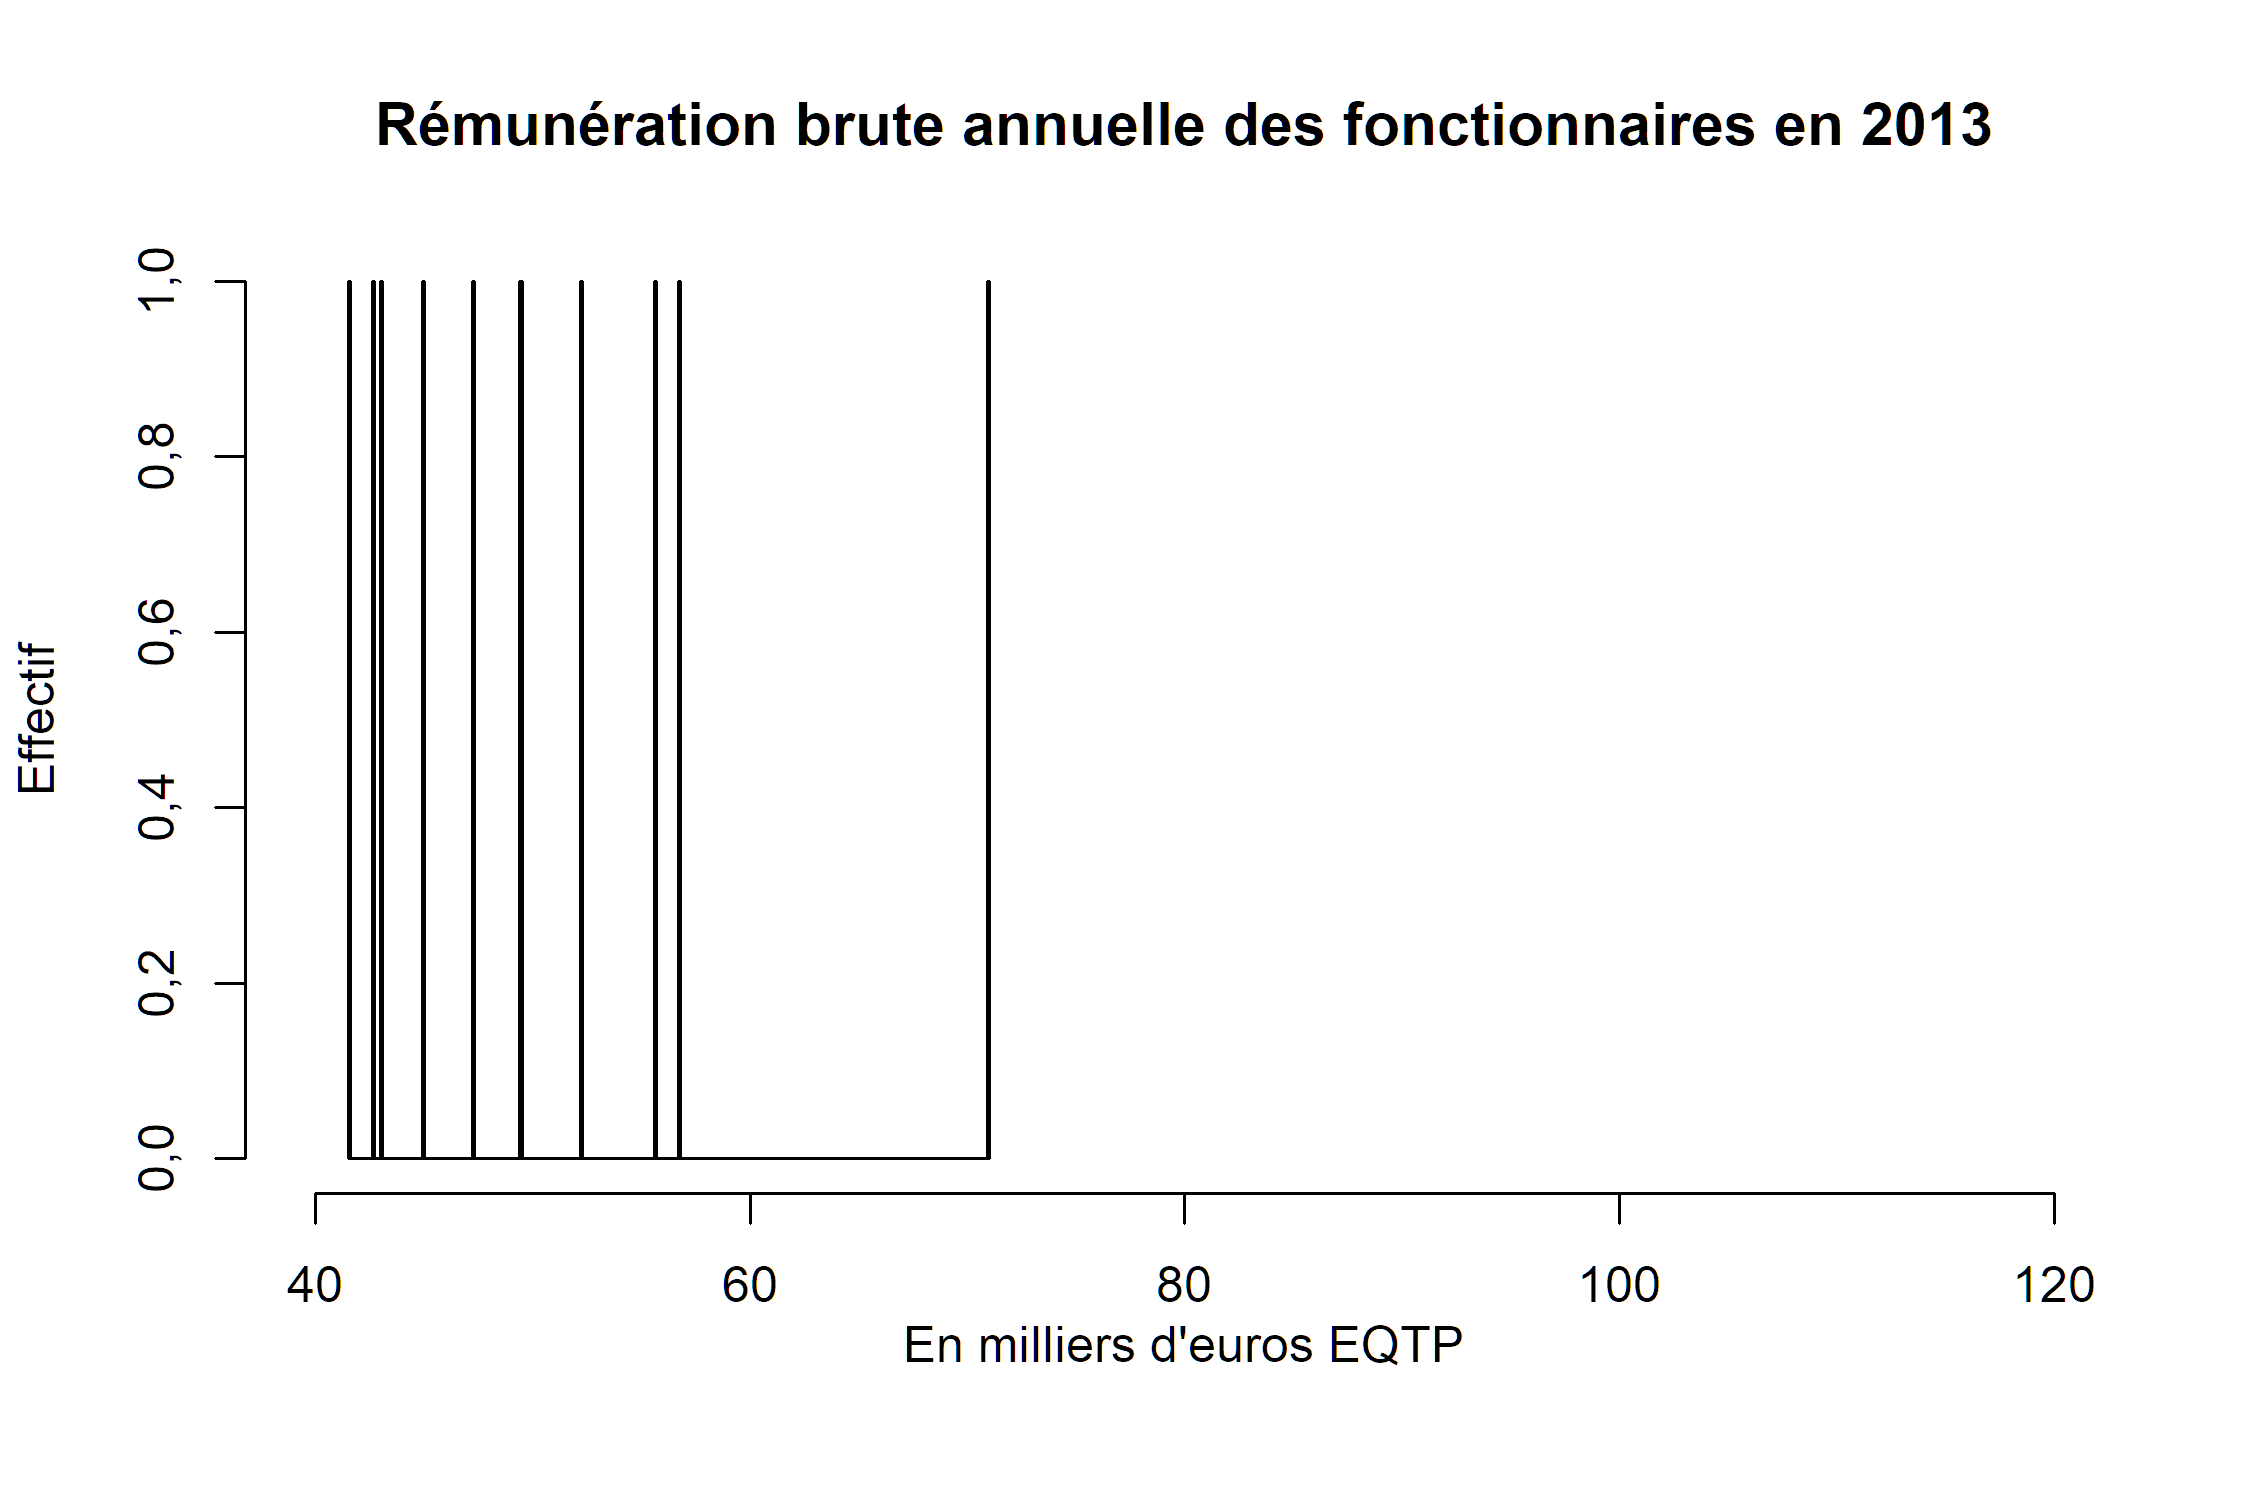
\includegraphics{altair_files/figure-latex/unnamed-chunk-76-2.png}

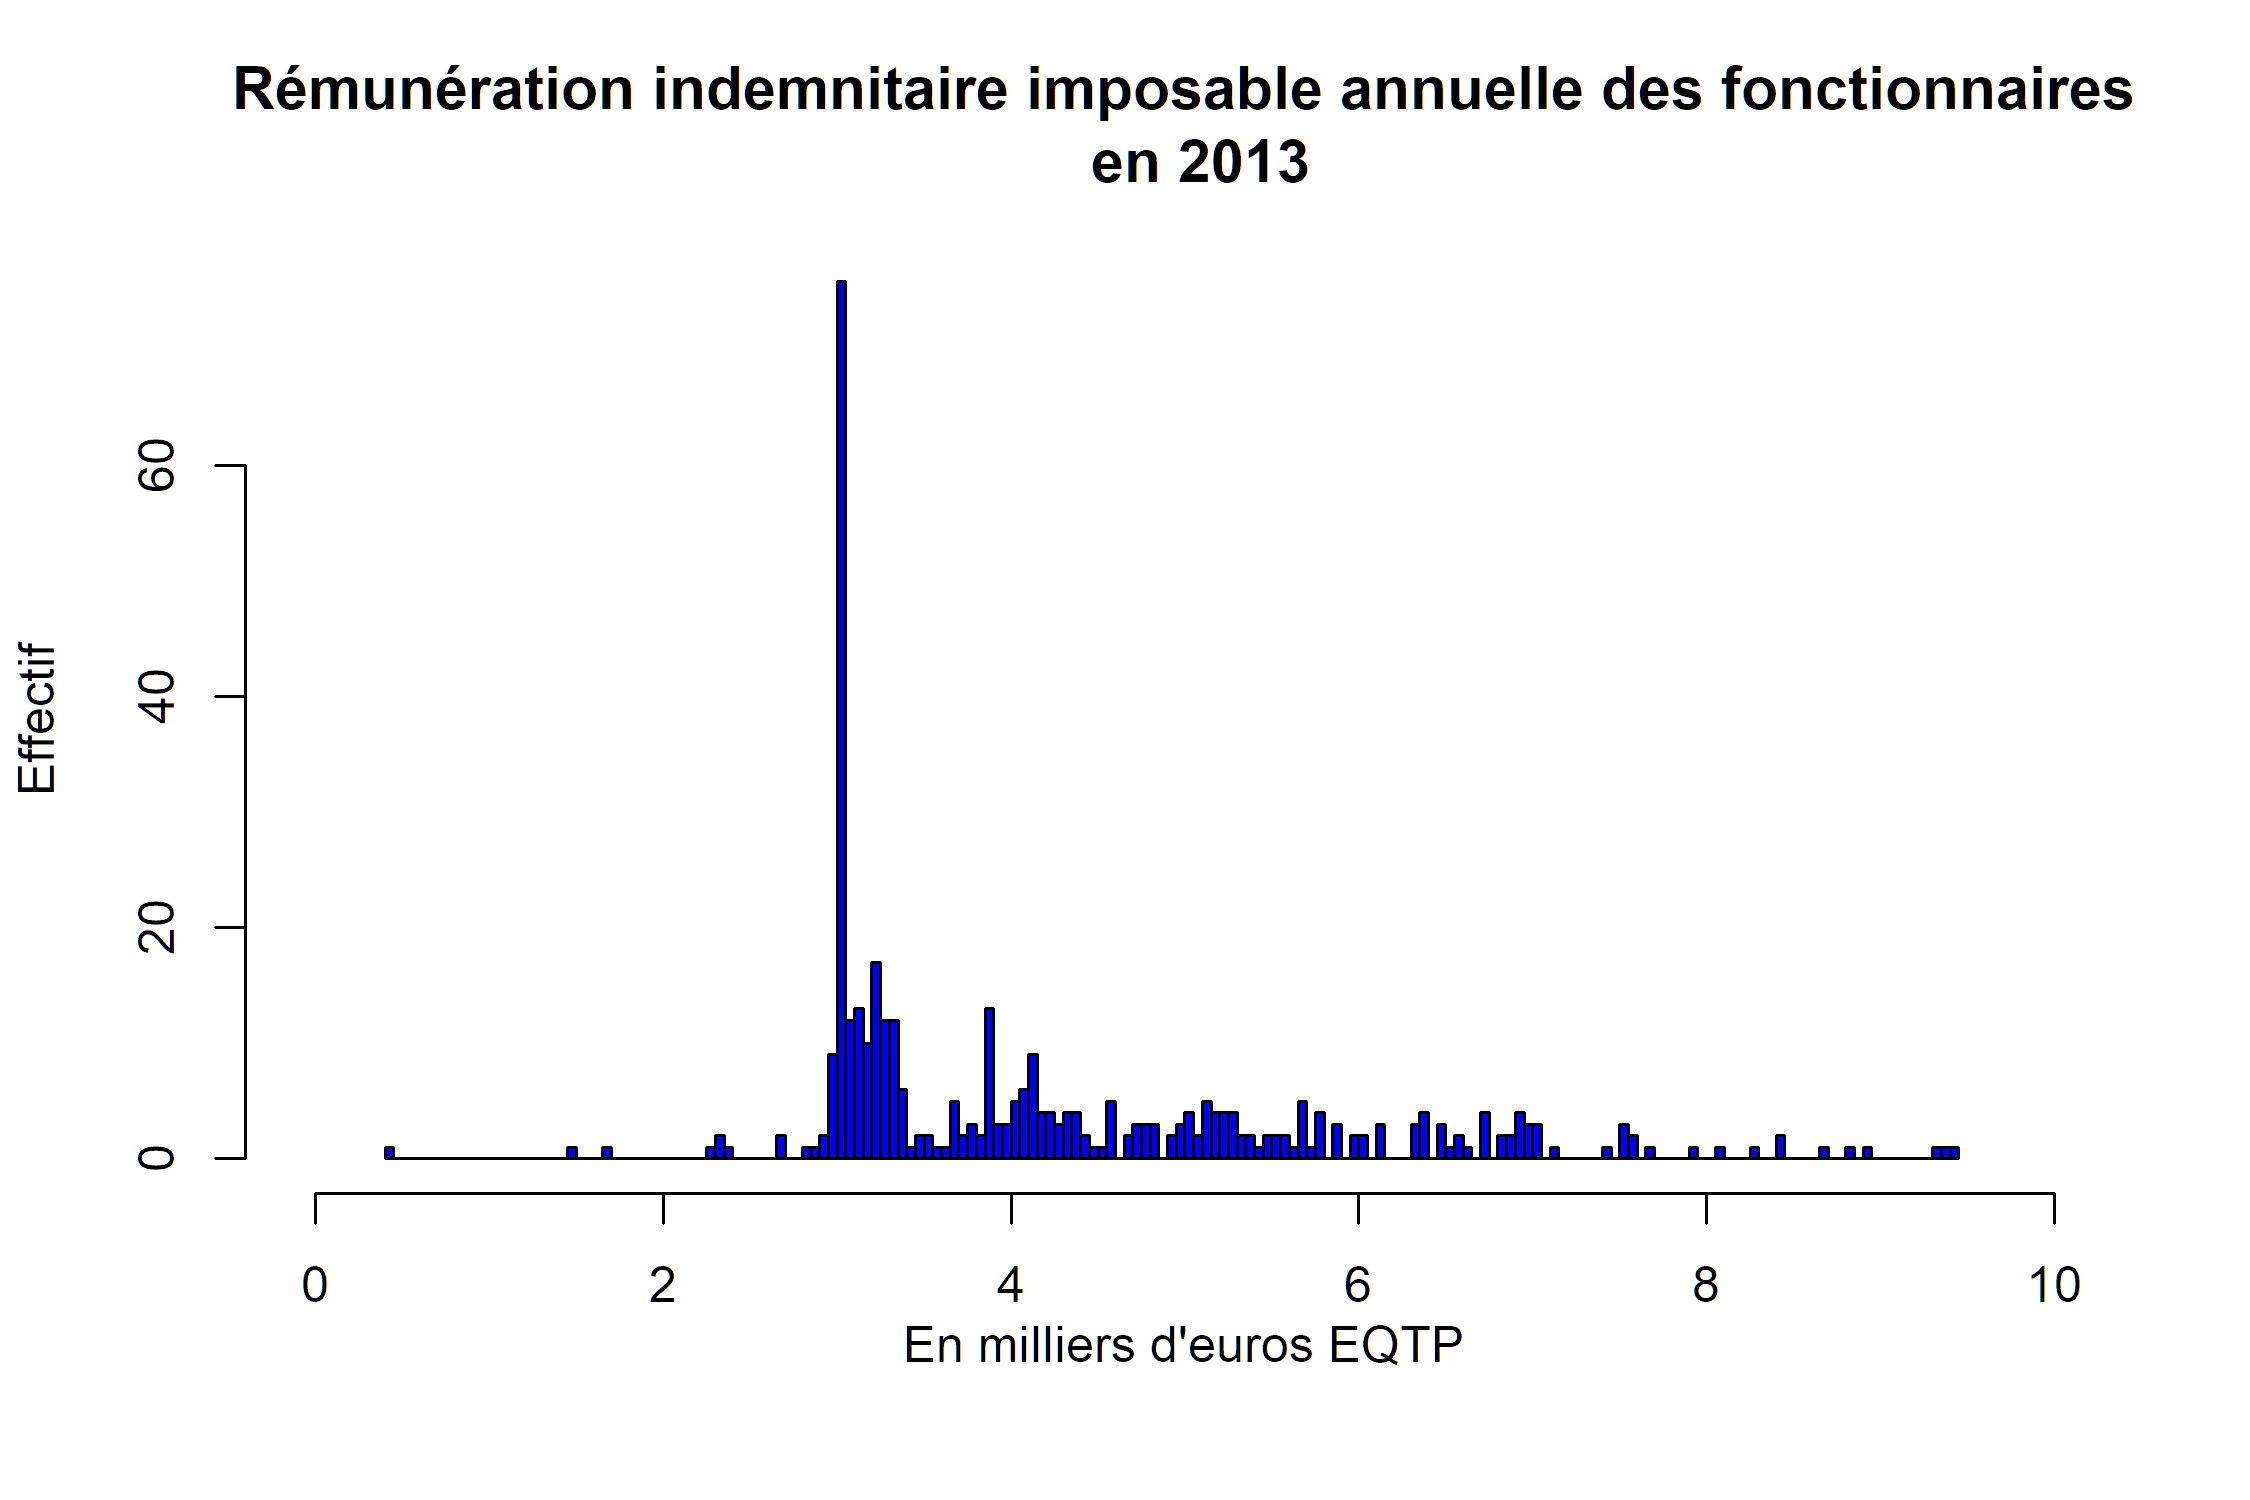
\includegraphics{altair_files/figure-latex/unnamed-chunk-76-3.png}

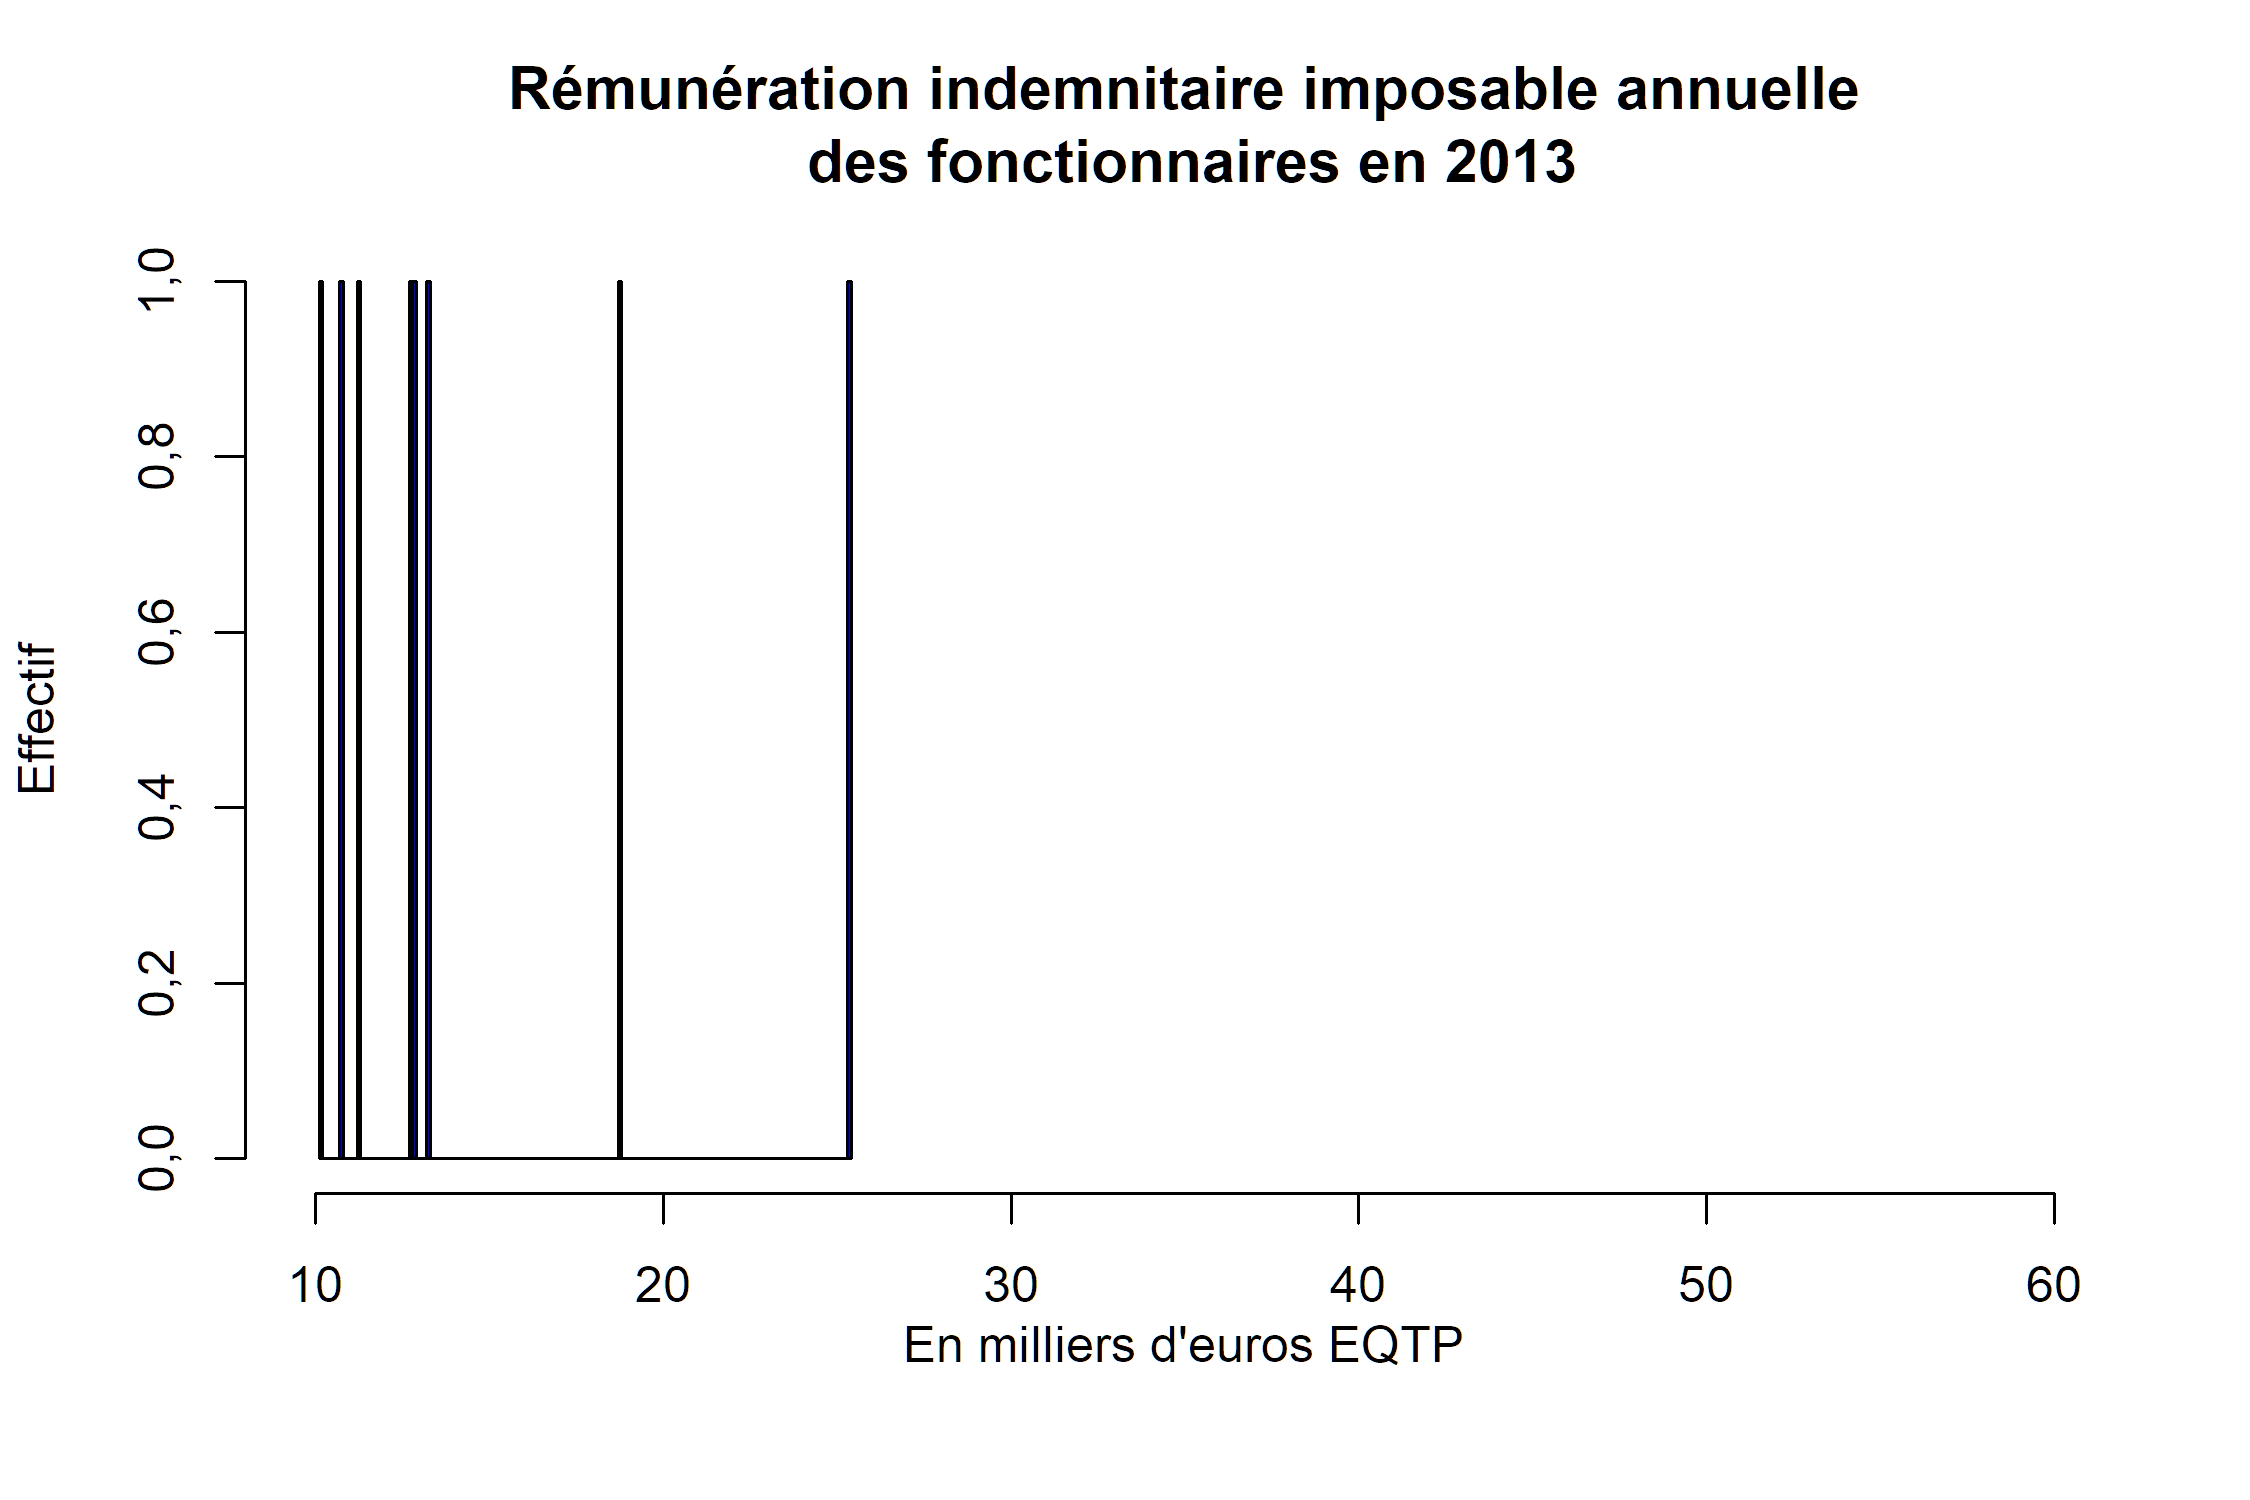
\includegraphics{altair_files/figure-latex/unnamed-chunk-76-4.png}

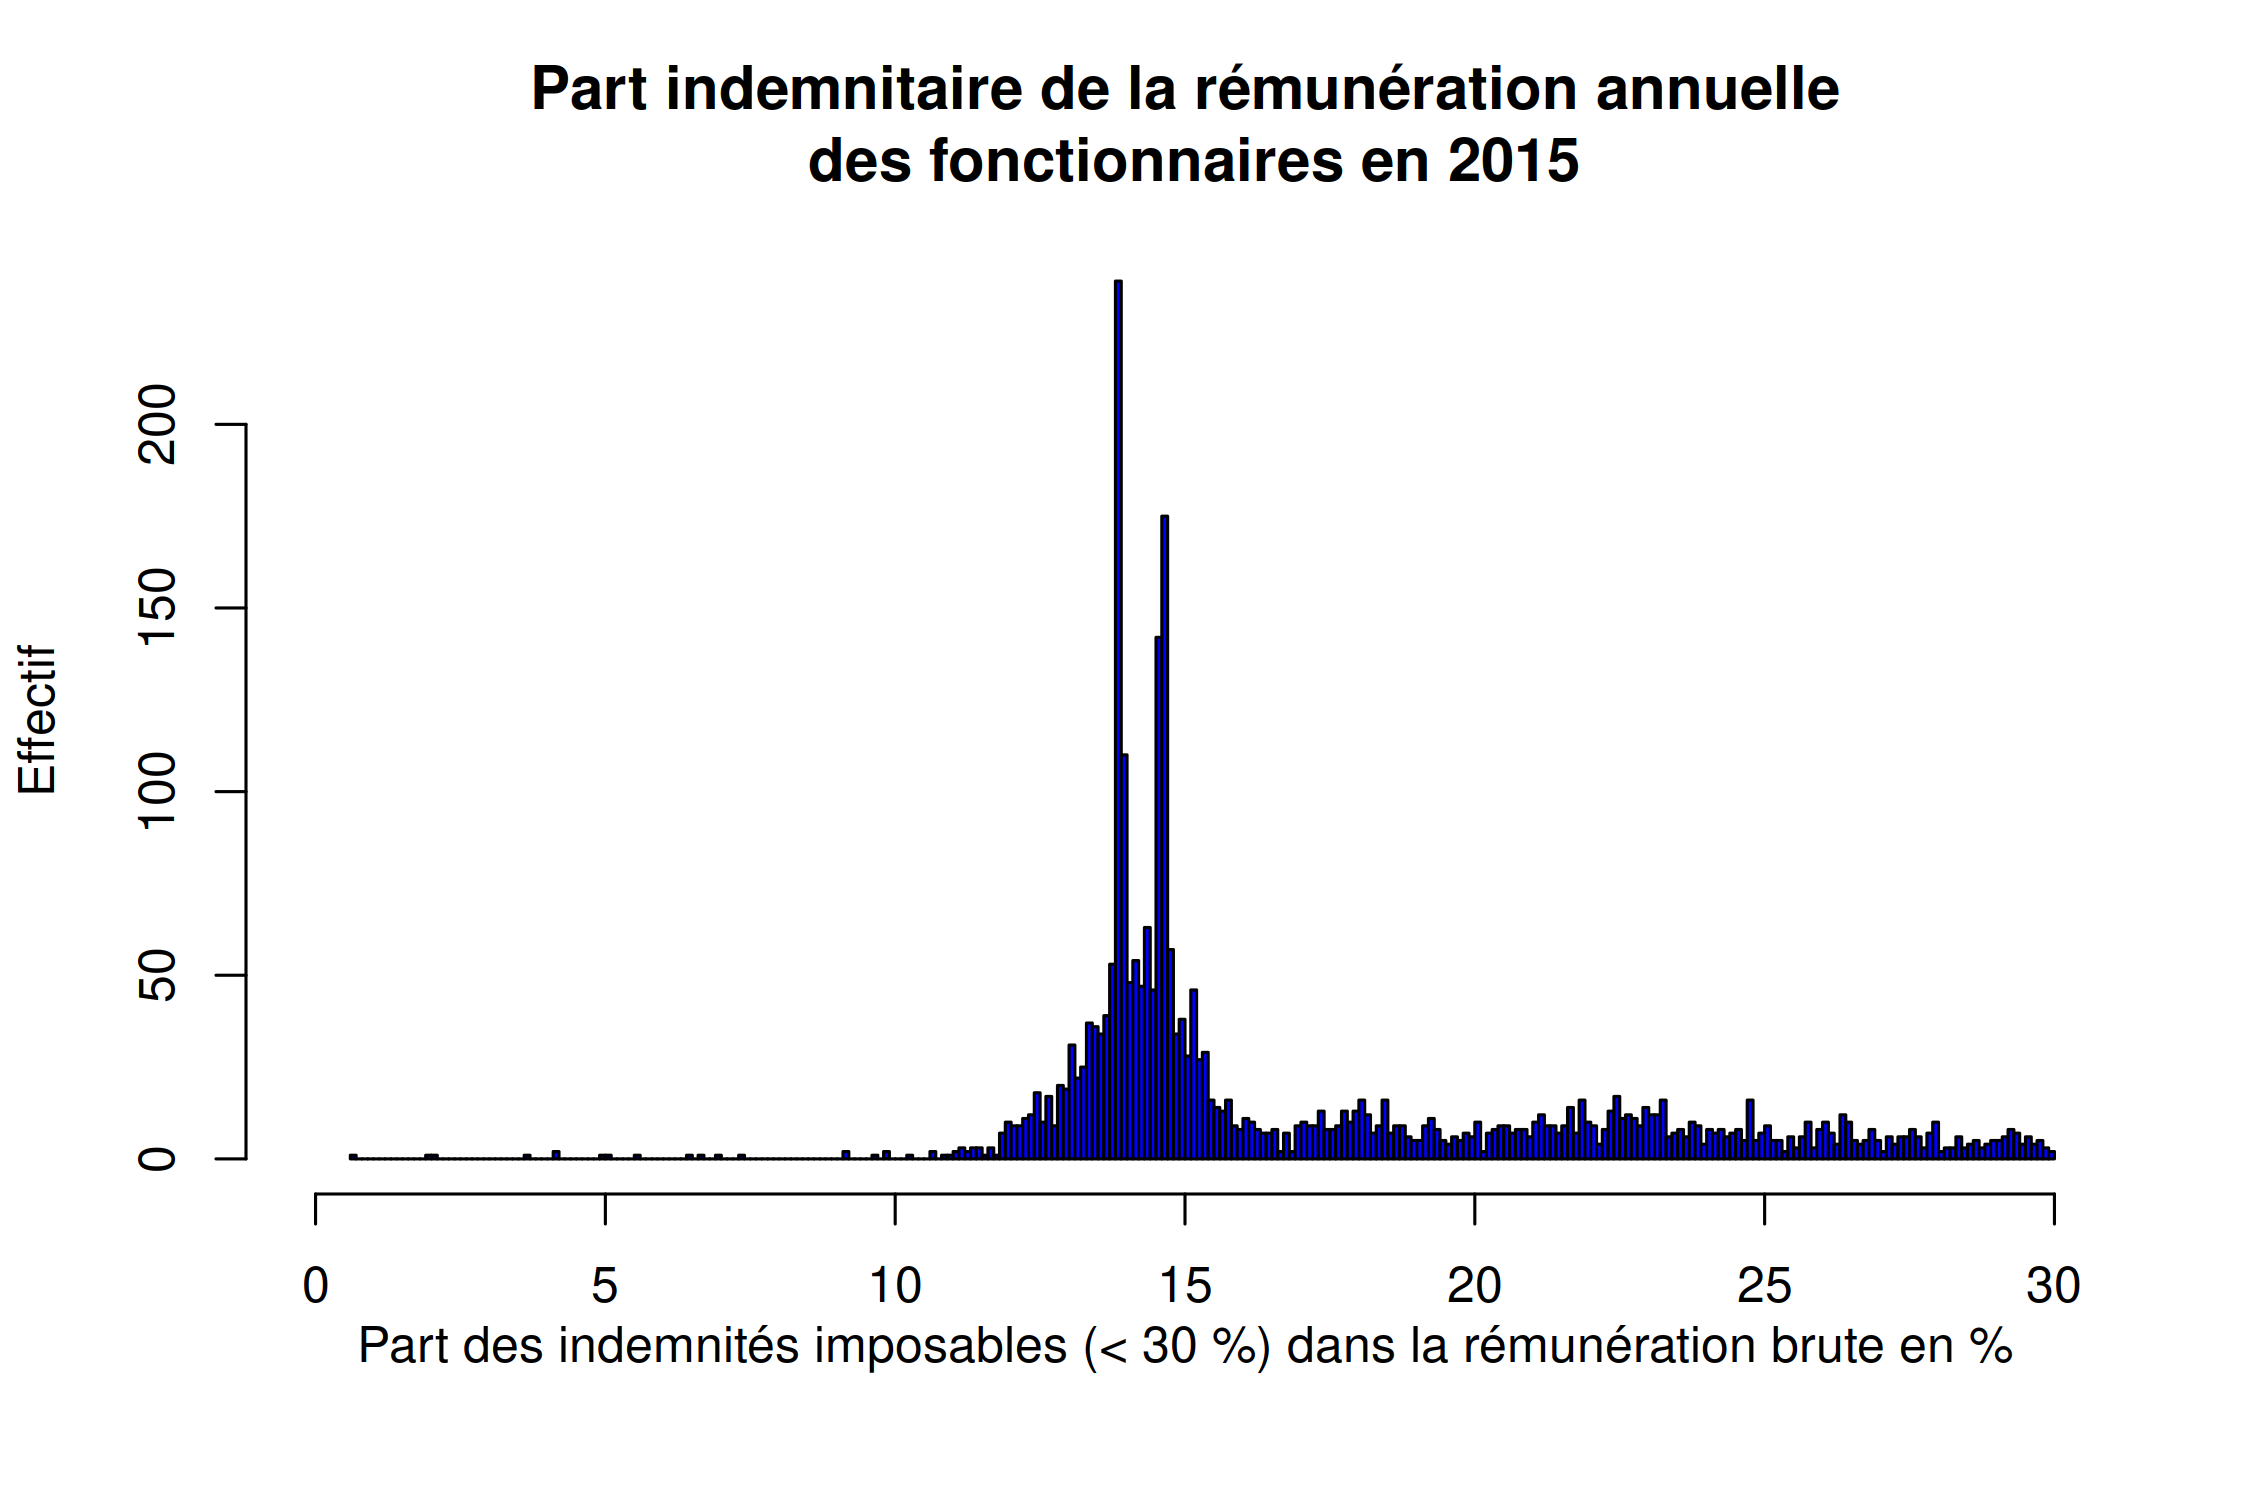
\includegraphics{altair_files/figure-latex/unnamed-chunk-76-5.png}

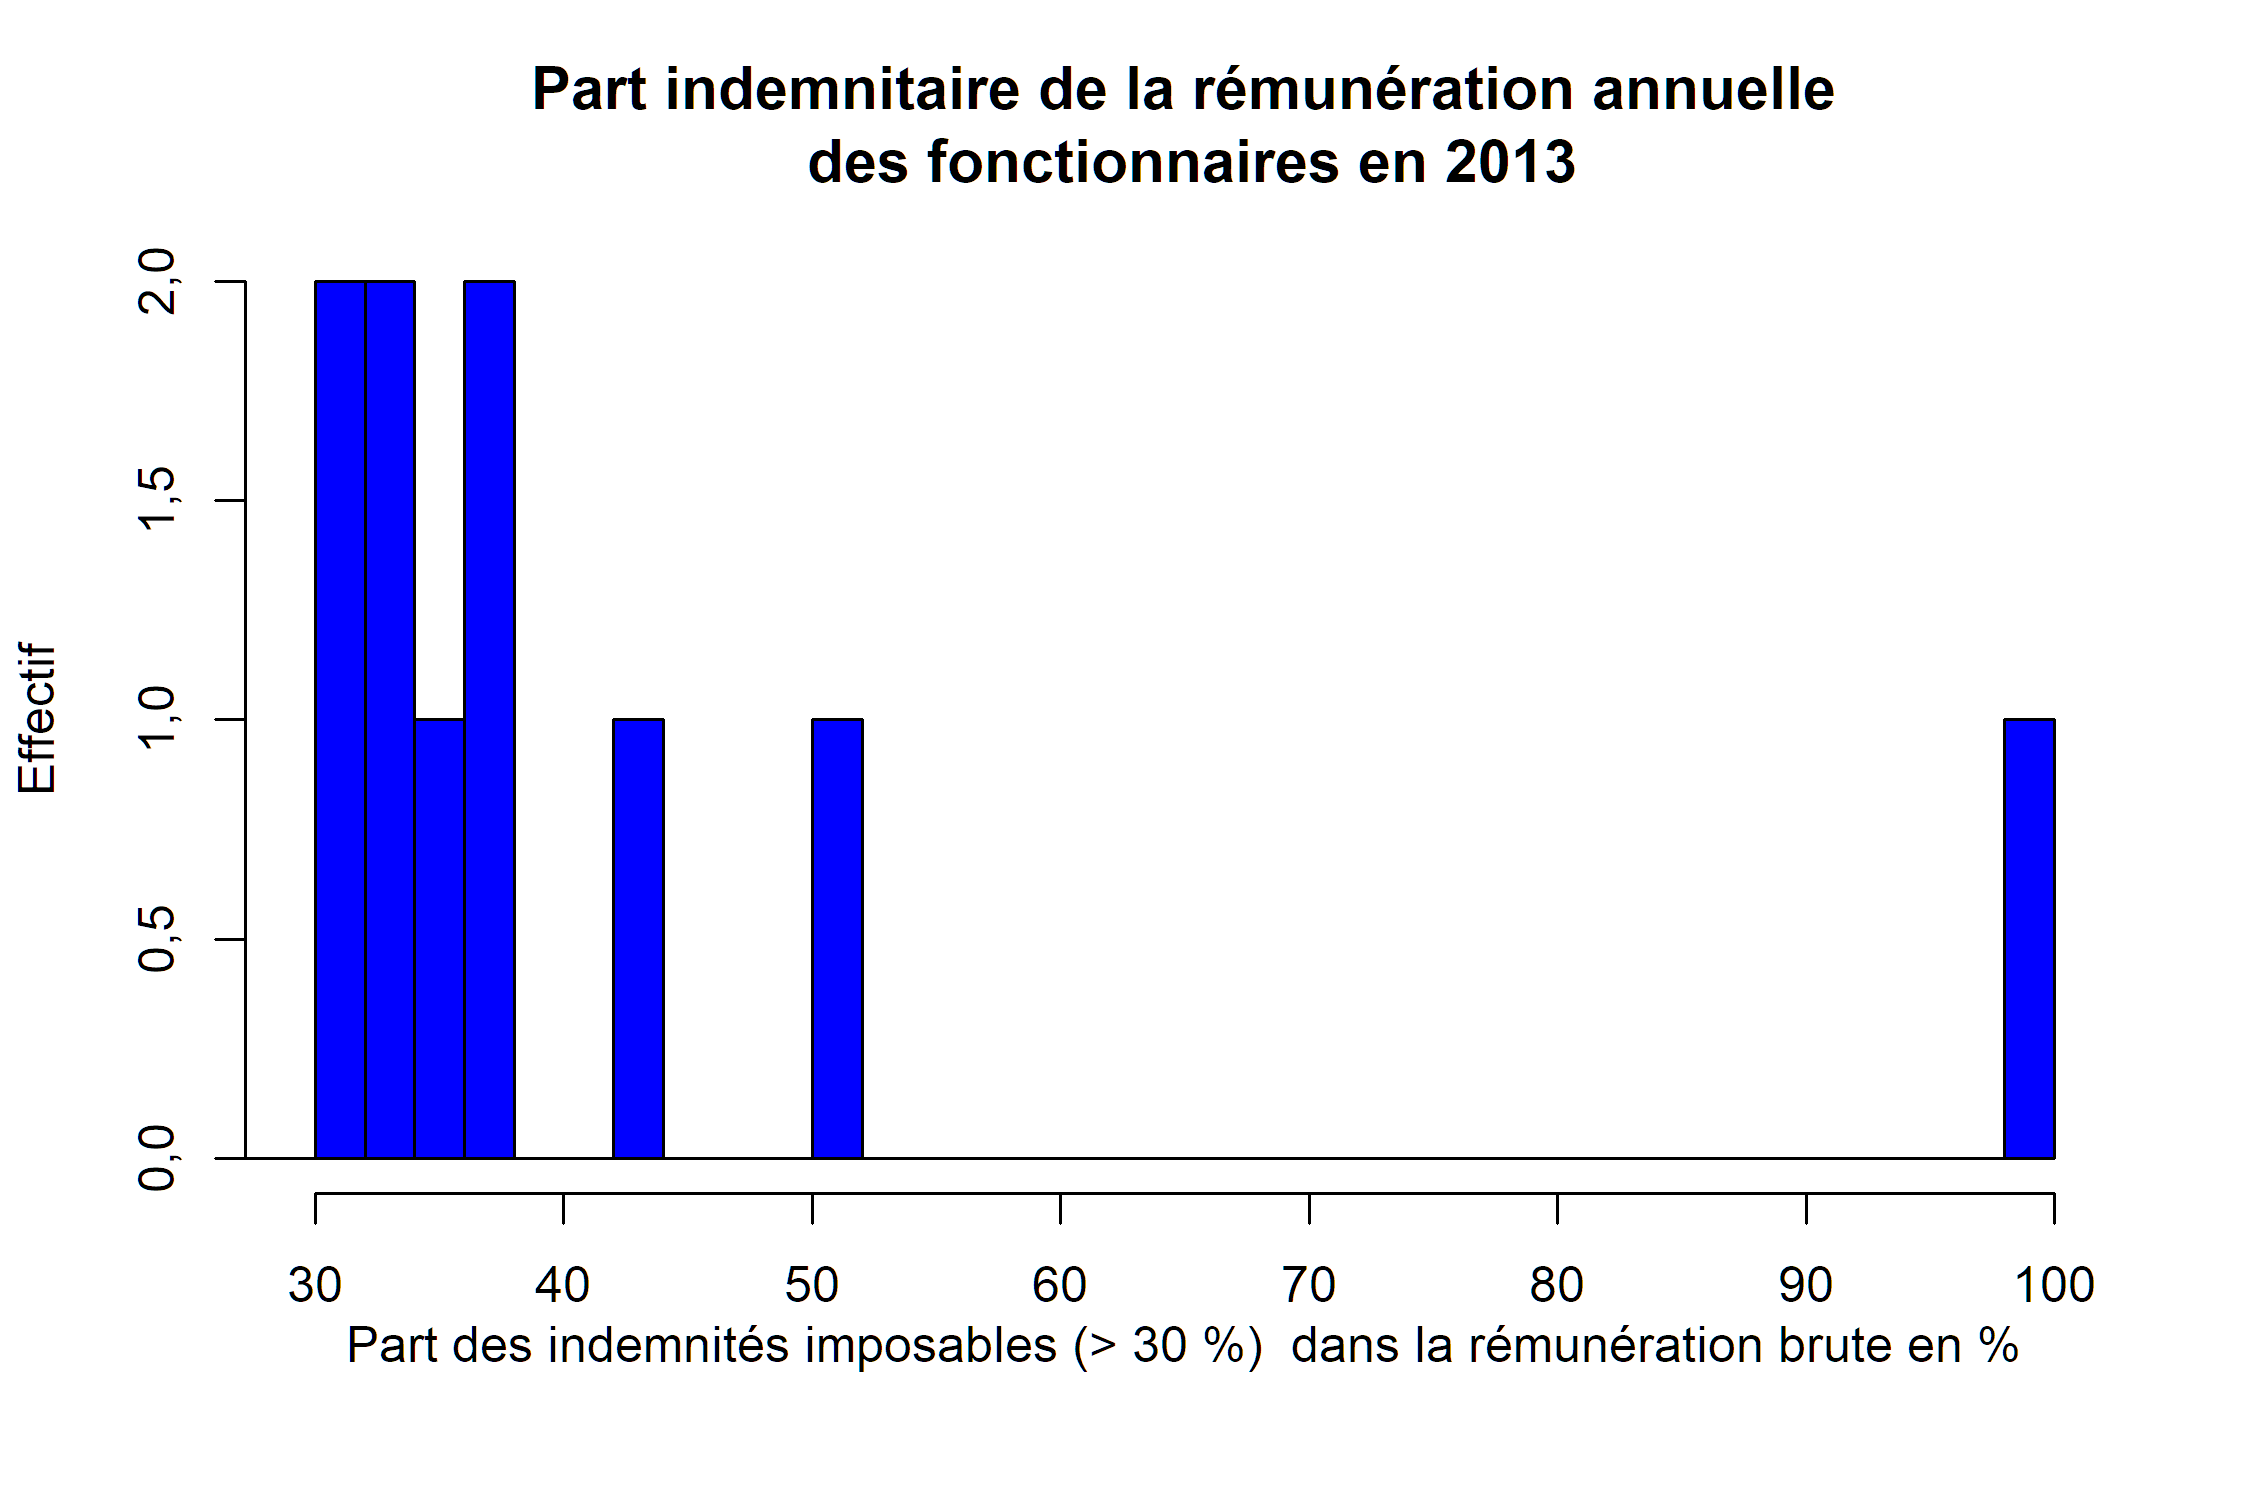
\includegraphics{altair_files/figure-latex/unnamed-chunk-76-6.png}

\textbf{Nota :}\\
\emph{Cet histogramme décrit l'évolution de la rémunération moyenne des
personnes en place (RMPP), définies comme présentes deux annees entières
consécutives avec la même quotité}\\
\emph{L'évolution de la RMPP permet d'étudier le glissement
vieillesse-technicité ``positif'', à effectifs constants sur deux
années}

\textbf{Effectif : 665 }

\textbf{Tests de cohérence}

Somme des rémunérations brutes versées aux personnels titulaires et
stagiaires :

~\emph{Tableau 3.2.1}

\begin{longtable}[]{@{}ll@{}}
\toprule
Agrégats & k€\tabularnewline
\midrule
\endhead
Brut annuel (bulletins) & 17 402 292,3\tabularnewline
Brut annuel (lignes) : & 17 324 086,3\tabularnewline
~dont ~~primes : & 2 336 908,6\tabularnewline
~dont ~autres rémunérations : &\tabularnewline
Part de primes en \% & 13,4\tabularnewline
\bottomrule
\end{longtable}

\textbf{Définitions :}

\emph{Brut annuel (bulletins)} : somme du champ \emph{Brut}\\
\emph{Brut annuel (lignes)} : somme du champ \emph{Montant} des lignes
de paye, dont :\\
\emph{Primes} : indemnités sauf remboursements, certaines IJSS,
Supplément familial de traitement et Indemnité de résidence\\
\emph{Autres rémunérations} : acomptes, retenues sur brut, rémunérations
diverses, rappels

\textbf{Tests de cohérence}

Somme des rémunérations brutes versées aux personnels (fonctionnaires) :

~\emph{Tableau 3.2.2}

\begin{longtable}[]{@{}ll@{}}
\toprule
Agrégats & k€\tabularnewline
\midrule
\endhead
Bulletins de paie & 17 402 292,3\tabularnewline
Lignes de paie & 17 324 086,3\tabularnewline
Difference & 78 206,0\tabularnewline
\bottomrule
\end{longtable}

A comparer aux soldes des comptes 6411, 6419 et 648 du compte de
gestion.

\textbf{Formation et distribution du salaire brut moyen par tête (SMPT)
en EQTP pour l'année 2014 }

~\emph{Tableau 3.2.3}

\begin{longtable}[]{@{}rrrrrr@{}}
\toprule
\begin{minipage}[b]{0.14\columnwidth}\raggedleft
Statistique\strut
\end{minipage} & \begin{minipage}[b]{0.23\columnwidth}\raggedleft
Traitement indiciaire\strut
\end{minipage} & \begin{minipage}[b]{0.07\columnwidth}\raggedleft
Primes\strut
\end{minipage} & \begin{minipage}[b]{0.22\columnwidth}\raggedleft
Autres rémunérations\strut
\end{minipage} & \begin{minipage}[b]{0.08\columnwidth}\raggedleft
Quotité\strut
\end{minipage} & \begin{minipage}[b]{0.09\columnwidth}\raggedleft
Effectif\strut
\end{minipage}\tabularnewline
\midrule
\endhead
\begin{minipage}[t]{0.14\columnwidth}\raggedleft
Minimum\strut
\end{minipage} & \begin{minipage}[t]{0.23\columnwidth}\raggedleft
3 982\strut
\end{minipage} & \begin{minipage}[t]{0.07\columnwidth}\raggedleft
427\strut
\end{minipage} & \begin{minipage}[t]{0.22\columnwidth}\raggedleft
0\strut
\end{minipage} & \begin{minipage}[t]{0.08\columnwidth}\raggedleft
0,33\strut
\end{minipage} & \begin{minipage}[t]{0.09\columnwidth}\raggedleft
\strut
\end{minipage}\tabularnewline
\begin{minipage}[t]{0.14\columnwidth}\raggedleft
1er quartile\strut
\end{minipage} & \begin{minipage}[t]{0.23\columnwidth}\raggedleft
17 569\strut
\end{minipage} & \begin{minipage}[t]{0.07\columnwidth}\raggedleft
2 681\strut
\end{minipage} & \begin{minipage}[t]{0.22\columnwidth}\raggedleft
0\strut
\end{minipage} & \begin{minipage}[t]{0.08\columnwidth}\raggedleft
0,9\strut
\end{minipage} & \begin{minipage}[t]{0.09\columnwidth}\raggedleft
\strut
\end{minipage}\tabularnewline
\begin{minipage}[t]{0.14\columnwidth}\raggedleft
Médiane\strut
\end{minipage} & \begin{minipage}[t]{0.23\columnwidth}\raggedleft
19 711\strut
\end{minipage} & \begin{minipage}[t]{0.07\columnwidth}\raggedleft
3 600\strut
\end{minipage} & \begin{minipage}[t]{0.22\columnwidth}\raggedleft
0\strut
\end{minipage} & \begin{minipage}[t]{0.08\columnwidth}\raggedleft
1\strut
\end{minipage} & \begin{minipage}[t]{0.09\columnwidth}\raggedleft
\strut
\end{minipage}\tabularnewline
\begin{minipage}[t]{0.14\columnwidth}\raggedleft
Moyenne\strut
\end{minipage} & \begin{minipage}[t]{0.23\columnwidth}\raggedleft
21 189\strut
\end{minipage} & \begin{minipage}[t]{0.07\columnwidth}\raggedleft
3 799\strut
\end{minipage} & \begin{minipage}[t]{0.22\columnwidth}\raggedleft
0\strut
\end{minipage} & \begin{minipage}[t]{0.08\columnwidth}\raggedleft
0,94\strut
\end{minipage} & \begin{minipage}[t]{0.09\columnwidth}\raggedleft
622\strut
\end{minipage}\tabularnewline
\begin{minipage}[t]{0.14\columnwidth}\raggedleft
3ème quartile\strut
\end{minipage} & \begin{minipage}[t]{0.23\columnwidth}\raggedleft
23 809\strut
\end{minipage} & \begin{minipage}[t]{0.07\columnwidth}\raggedleft
4 370\strut
\end{minipage} & \begin{minipage}[t]{0.22\columnwidth}\raggedleft
0\strut
\end{minipage} & \begin{minipage}[t]{0.08\columnwidth}\raggedleft
1\strut
\end{minipage} & \begin{minipage}[t]{0.09\columnwidth}\raggedleft
\strut
\end{minipage}\tabularnewline
\begin{minipage}[t]{0.14\columnwidth}\raggedleft
Maximum\strut
\end{minipage} & \begin{minipage}[t]{0.23\columnwidth}\raggedleft
58 036\strut
\end{minipage} & \begin{minipage}[t]{0.07\columnwidth}\raggedleft
26 284\strut
\end{minipage} & \begin{minipage}[t]{0.22\columnwidth}\raggedleft
0\strut
\end{minipage} & \begin{minipage}[t]{0.08\columnwidth}\raggedleft
1\strut
\end{minipage} & \begin{minipage}[t]{0.09\columnwidth}\raggedleft
\strut
\end{minipage}\tabularnewline
\bottomrule
\end{longtable}

~\emph{Tableau 3.2.4}

\begin{longtable}[]{@{}rrrrrrr@{}}
\toprule
\begin{minipage}[b]{0.11\columnwidth}\raggedleft
Statistique\strut
\end{minipage} & \begin{minipage}[b]{0.20\columnwidth}\raggedleft
Total lignes hors rappels\strut
\end{minipage} & \begin{minipage}[b]{0.09\columnwidth}\raggedleft
Total brut\strut
\end{minipage} & \begin{minipage}[b]{0.14\columnwidth}\raggedleft
SMPT brut en EQTP\strut
\end{minipage} & \begin{minipage}[b]{0.14\columnwidth}\raggedleft
Part indemnitaire\strut
\end{minipage} & \begin{minipage}[b]{0.06\columnwidth}\raggedleft
Quotité\strut
\end{minipage} & \begin{minipage}[b]{0.07\columnwidth}\raggedleft
Effectif\strut
\end{minipage}\tabularnewline
\midrule
\endhead
\begin{minipage}[t]{0.11\columnwidth}\raggedleft
Minimum\strut
\end{minipage} & \begin{minipage}[t]{0.20\columnwidth}\raggedleft
6 859\strut
\end{minipage} & \begin{minipage}[t]{0.09\columnwidth}\raggedleft
7 010\strut
\end{minipage} & \begin{minipage}[t]{0.14\columnwidth}\raggedleft
94 008\strut
\end{minipage} & \begin{minipage}[t]{0.14\columnwidth}\raggedleft
6\strut
\end{minipage} & \begin{minipage}[t]{0.06\columnwidth}\raggedleft
0,33\strut
\end{minipage} & \begin{minipage}[t]{0.07\columnwidth}\raggedleft
\strut
\end{minipage}\tabularnewline
\begin{minipage}[t]{0.11\columnwidth}\raggedleft
1er quartile\strut
\end{minipage} & \begin{minipage}[t]{0.20\columnwidth}\raggedleft
22 775\strut
\end{minipage} & \begin{minipage}[t]{0.09\columnwidth}\raggedleft
22 737\strut
\end{minipage} & \begin{minipage}[t]{0.14\columnwidth}\raggedleft
281 755\strut
\end{minipage} & \begin{minipage}[t]{0.14\columnwidth}\raggedleft
9,6\strut
\end{minipage} & \begin{minipage}[t]{0.06\columnwidth}\raggedleft
0,9\strut
\end{minipage} & \begin{minipage}[t]{0.07\columnwidth}\raggedleft
\strut
\end{minipage}\tabularnewline
\begin{minipage}[t]{0.11\columnwidth}\raggedleft
Médiane\strut
\end{minipage} & \begin{minipage}[t]{0.20\columnwidth}\raggedleft
26 374\strut
\end{minipage} & \begin{minipage}[t]{0.09\columnwidth}\raggedleft
26 612\strut
\end{minipage} & \begin{minipage}[t]{0.14\columnwidth}\raggedleft
332 613\strut
\end{minipage} & \begin{minipage}[t]{0.14\columnwidth}\raggedleft
13\strut
\end{minipage} & \begin{minipage}[t]{0.06\columnwidth}\raggedleft
1\strut
\end{minipage} & \begin{minipage}[t]{0.07\columnwidth}\raggedleft
\strut
\end{minipage}\tabularnewline
\begin{minipage}[t]{0.11\columnwidth}\raggedleft
Moyenne\strut
\end{minipage} & \begin{minipage}[t]{0.20\columnwidth}\raggedleft
28 253\strut
\end{minipage} & \begin{minipage}[t]{0.09\columnwidth}\raggedleft
28 381\strut
\end{minipage} & \begin{minipage}[t]{0.14\columnwidth}\raggedleft
355 979\strut
\end{minipage} & \begin{minipage}[t]{0.14\columnwidth}\raggedleft
13\strut
\end{minipage} & \begin{minipage}[t]{0.06\columnwidth}\raggedleft
0,94\strut
\end{minipage} & \begin{minipage}[t]{0.07\columnwidth}\raggedleft
622\strut
\end{minipage}\tabularnewline
\begin{minipage}[t]{0.11\columnwidth}\raggedleft
3ème quartile\strut
\end{minipage} & \begin{minipage}[t]{0.20\columnwidth}\raggedleft
31 806\strut
\end{minipage} & \begin{minipage}[t]{0.09\columnwidth}\raggedleft
32 014\strut
\end{minipage} & \begin{minipage}[t]{0.14\columnwidth}\raggedleft
412 427\strut
\end{minipage} & \begin{minipage}[t]{0.14\columnwidth}\raggedleft
16\strut
\end{minipage} & \begin{minipage}[t]{0.06\columnwidth}\raggedleft
1\strut
\end{minipage} & \begin{minipage}[t]{0.07\columnwidth}\raggedleft
\strut
\end{minipage}\tabularnewline
\begin{minipage}[t]{0.11\columnwidth}\raggedleft
Maximum\strut
\end{minipage} & \begin{minipage}[t]{0.20\columnwidth}\raggedleft
89 500\strut
\end{minipage} & \begin{minipage}[t]{0.09\columnwidth}\raggedleft
92 143\strut
\end{minipage} & \begin{minipage}[t]{0.14\columnwidth}\raggedleft
1 084 906\strut
\end{minipage} & \begin{minipage}[t]{0.14\columnwidth}\raggedleft
76\strut
\end{minipage} & \begin{minipage}[t]{0.06\columnwidth}\raggedleft
1\strut
\end{minipage} & \begin{minipage}[t]{0.07\columnwidth}\raggedleft
\strut
\end{minipage}\tabularnewline
\bottomrule
\end{longtable}

\emph{Hors vacataires identifiés, assistantes maternelles, élus locaux
et pour les postes actifs non annexes}

\textbf{Categorie A}

~\emph{Tableau 3.2.5}

\begin{longtable}[]{@{}rrrrr@{}}
\toprule
Statistique & Traitement indiciaire & Primes & Autres rémunérations &
Quotité\tabularnewline
\midrule
\endhead
Minimum & 7 731 & 1 122 & 0 & 0,4\tabularnewline
1er quartile & 21 244 & 3 372 & 0 & 0,8\tabularnewline
Médiane & 25 717 & 3 798 & 0 & 1\tabularnewline
Moyenne & 25 741 & 4 688 & 0 & 0,9\tabularnewline
3ème quartile & 29 973 & 5 119 & 0 & 1\tabularnewline
Maximum & 58 036 & 26 284 & 0 & 1\tabularnewline
\bottomrule
\end{longtable}

~\emph{Tableau 3.2.6}

\begin{longtable}[]{@{}rrrrr@{}}
\toprule
\begin{minipage}[b]{0.14\columnwidth}\raggedleft
Statistique\strut
\end{minipage} & \begin{minipage}[b]{0.20\columnwidth}\raggedleft
Total rémunérations\strut
\end{minipage} & \begin{minipage}[b]{0.25\columnwidth}\raggedleft
Total rémunérations EQTP\strut
\end{minipage} & \begin{minipage}[b]{0.18\columnwidth}\raggedleft
Part indemnitaire\strut
\end{minipage} & \begin{minipage}[b]{0.08\columnwidth}\raggedleft
Quotité\strut
\end{minipage}\tabularnewline
\midrule
\endhead
\begin{minipage}[t]{0.14\columnwidth}\raggedleft
Minimum\strut
\end{minipage} & \begin{minipage}[t]{0.20\columnwidth}\raggedleft
11 125\strut
\end{minipage} & \begin{minipage}[t]{0.25\columnwidth}\raggedleft
156 775\strut
\end{minipage} & \begin{minipage}[t]{0.18\columnwidth}\raggedleft
6,8\strut
\end{minipage} & \begin{minipage}[t]{0.08\columnwidth}\raggedleft
0,4\strut
\end{minipage}\tabularnewline
\begin{minipage}[t]{0.14\columnwidth}\raggedleft
1er quartile\strut
\end{minipage} & \begin{minipage}[t]{0.20\columnwidth}\raggedleft
27 904\strut
\end{minipage} & \begin{minipage}[t]{0.25\columnwidth}\raggedleft
376 500\strut
\end{minipage} & \begin{minipage}[t]{0.18\columnwidth}\raggedleft
10\strut
\end{minipage} & \begin{minipage}[t]{0.08\columnwidth}\raggedleft
0,8\strut
\end{minipage}\tabularnewline
\begin{minipage}[t]{0.14\columnwidth}\raggedleft
Médiane\strut
\end{minipage} & \begin{minipage}[t]{0.20\columnwidth}\raggedleft
33 970\strut
\end{minipage} & \begin{minipage}[t]{0.25\columnwidth}\raggedleft
434 226\strut
\end{minipage} & \begin{minipage}[t]{0.18\columnwidth}\raggedleft
12\strut
\end{minipage} & \begin{minipage}[t]{0.08\columnwidth}\raggedleft
1\strut
\end{minipage}\tabularnewline
\begin{minipage}[t]{0.14\columnwidth}\raggedleft
Moyenne\strut
\end{minipage} & \begin{minipage}[t]{0.20\columnwidth}\raggedleft
35 074\strut
\end{minipage} & \begin{minipage}[t]{0.25\columnwidth}\raggedleft
451 715\strut
\end{minipage} & \begin{minipage}[t]{0.18\columnwidth}\raggedleft
13\strut
\end{minipage} & \begin{minipage}[t]{0.08\columnwidth}\raggedleft
0,9\strut
\end{minipage}\tabularnewline
\begin{minipage}[t]{0.14\columnwidth}\raggedleft
3ème quartile\strut
\end{minipage} & \begin{minipage}[t]{0.20\columnwidth}\raggedleft
39 148\strut
\end{minipage} & \begin{minipage}[t]{0.25\columnwidth}\raggedleft
496 759\strut
\end{minipage} & \begin{minipage}[t]{0.18\columnwidth}\raggedleft
14\strut
\end{minipage} & \begin{minipage}[t]{0.08\columnwidth}\raggedleft
1\strut
\end{minipage}\tabularnewline
\begin{minipage}[t]{0.14\columnwidth}\raggedleft
Maximum\strut
\end{minipage} & \begin{minipage}[t]{0.20\columnwidth}\raggedleft
92 143\strut
\end{minipage} & \begin{minipage}[t]{0.25\columnwidth}\raggedleft
1 084 906\strut
\end{minipage} & \begin{minipage}[t]{0.18\columnwidth}\raggedleft
49\strut
\end{minipage} & \begin{minipage}[t]{0.08\columnwidth}\raggedleft
1\strut
\end{minipage}\tabularnewline
\bottomrule
\end{longtable}

\textbf{Effectif : 223 }

\textbf{Categorie B}

~\emph{Tableau 3.2.7}

\begin{longtable}[]{@{}rrrrr@{}}
\toprule
Statistique & Traitement indiciaire & Primes & Autres rémunérations &
Quotité\tabularnewline
\midrule
\endhead
Minimum & 13 533 & 1 408 & 0 & 0,58\tabularnewline
1er quartile & 20 931 & 2 842 & 0 & 1\tabularnewline
Médiane & 23 773 & 3 365 & 0 & 1\tabularnewline
Moyenne & 24 338 & 4 061 & 0 & 0,95\tabularnewline
3ème quartile & 28 989 & 4 396 & 0 & 1\tabularnewline
Maximum & 37 339 & 11 566 & 0 & 1\tabularnewline
\bottomrule
\end{longtable}

~\emph{Tableau 3.2.8}

\begin{longtable}[]{@{}rrrrr@{}}
\toprule
\begin{minipage}[b]{0.12\columnwidth}\raggedleft
Statistique\strut
\end{minipage} & \begin{minipage}[b]{0.17\columnwidth}\raggedleft
Total rémunérations\strut
\end{minipage} & \begin{minipage}[b]{0.21\columnwidth}\raggedleft
Total rémunérations EQTP\strut
\end{minipage} & \begin{minipage}[b]{0.31\columnwidth}\raggedleft
Part de la rémunération indemnitaire\strut
\end{minipage} & \begin{minipage}[b]{0.07\columnwidth}\raggedleft
Quotité\strut
\end{minipage}\tabularnewline
\midrule
\endhead
\begin{minipage}[t]{0.12\columnwidth}\raggedleft
Minimum\strut
\end{minipage} & \begin{minipage}[t]{0.17\columnwidth}\raggedleft
17 833\strut
\end{minipage} & \begin{minipage}[t]{0.21\columnwidth}\raggedleft
229 766\strut
\end{minipage} & \begin{minipage}[t]{0.31\columnwidth}\raggedleft
6,9\strut
\end{minipage} & \begin{minipage}[t]{0.07\columnwidth}\raggedleft
0,58\strut
\end{minipage}\tabularnewline
\begin{minipage}[t]{0.12\columnwidth}\raggedleft
1er quartile\strut
\end{minipage} & \begin{minipage}[t]{0.17\columnwidth}\raggedleft
26 661\strut
\end{minipage} & \begin{minipage}[t]{0.21\columnwidth}\raggedleft
327 887\strut
\end{minipage} & \begin{minipage}[t]{0.31\columnwidth}\raggedleft
9\strut
\end{minipage} & \begin{minipage}[t]{0.07\columnwidth}\raggedleft
1\strut
\end{minipage}\tabularnewline
\begin{minipage}[t]{0.12\columnwidth}\raggedleft
Médiane\strut
\end{minipage} & \begin{minipage}[t]{0.17\columnwidth}\raggedleft
30 928\strut
\end{minipage} & \begin{minipage}[t]{0.21\columnwidth}\raggedleft
390 585\strut
\end{minipage} & \begin{minipage}[t]{0.31\columnwidth}\raggedleft
11\strut
\end{minipage} & \begin{minipage}[t]{0.07\columnwidth}\raggedleft
1\strut
\end{minipage}\tabularnewline
\begin{minipage}[t]{0.12\columnwidth}\raggedleft
Moyenne\strut
\end{minipage} & \begin{minipage}[t]{0.17\columnwidth}\raggedleft
31 047\strut
\end{minipage} & \begin{minipage}[t]{0.21\columnwidth}\raggedleft
379 234\strut
\end{minipage} & \begin{minipage}[t]{0.31\columnwidth}\raggedleft
13\strut
\end{minipage} & \begin{minipage}[t]{0.07\columnwidth}\raggedleft
0,95\strut
\end{minipage}\tabularnewline
\begin{minipage}[t]{0.12\columnwidth}\raggedleft
3ème quartile\strut
\end{minipage} & \begin{minipage}[t]{0.17\columnwidth}\raggedleft
35 837\strut
\end{minipage} & \begin{minipage}[t]{0.21\columnwidth}\raggedleft
432 739\strut
\end{minipage} & \begin{minipage}[t]{0.31\columnwidth}\raggedleft
14\strut
\end{minipage} & \begin{minipage}[t]{0.07\columnwidth}\raggedleft
1\strut
\end{minipage}\tabularnewline
\begin{minipage}[t]{0.12\columnwidth}\raggedleft
Maximum\strut
\end{minipage} & \begin{minipage}[t]{0.17\columnwidth}\raggedleft
47 552\strut
\end{minipage} & \begin{minipage}[t]{0.21\columnwidth}\raggedleft
559 881\strut
\end{minipage} & \begin{minipage}[t]{0.31\columnwidth}\raggedleft
34\strut
\end{minipage} & \begin{minipage}[t]{0.07\columnwidth}\raggedleft
1\strut
\end{minipage}\tabularnewline
\bottomrule
\end{longtable}

\textbf{Effectif : 61 }

\textbf{Categorie C}

~\emph{Tableau 3.2.9}

\begin{longtable}[]{@{}rrrrr@{}}
\toprule
Statistique & Traitement indiciaire & Primes & Autres rémunérations &
Quotité\tabularnewline
\midrule
\endhead
Minimum & 4 574 & 737 & 0 & 0,46\tabularnewline
1er quartile & 17 359 & 1 663 & 0 & 1\tabularnewline
Médiane & 17 632 & 3 445 & 0 & 1\tabularnewline
Moyenne & 17 846 & 3 209 & 0 & 0,95\tabularnewline
3ème quartile & 19 563 & 4 226 & 0 & 1\tabularnewline
Maximum & 25 351 & 15 067 & 0 & 1\tabularnewline
\bottomrule
\end{longtable}

~\emph{Tableau 3.2.10}

\begin{longtable}[]{@{}rrrrr@{}}
\toprule
\begin{minipage}[b]{0.12\columnwidth}\raggedleft
Statistique\strut
\end{minipage} & \begin{minipage}[b]{0.17\columnwidth}\raggedleft
Total rémunérations\strut
\end{minipage} & \begin{minipage}[b]{0.21\columnwidth}\raggedleft
Total rémunérations EQTP\strut
\end{minipage} & \begin{minipage}[b]{0.31\columnwidth}\raggedleft
Part de la rémunération indemnitaire\strut
\end{minipage} & \begin{minipage}[b]{0.07\columnwidth}\raggedleft
Quotité\strut
\end{minipage}\tabularnewline
\midrule
\endhead
\begin{minipage}[t]{0.12\columnwidth}\raggedleft
Minimum\strut
\end{minipage} & \begin{minipage}[t]{0.17\columnwidth}\raggedleft
8 032\strut
\end{minipage} & \begin{minipage}[t]{0.21\columnwidth}\raggedleft
94 573\strut
\end{minipage} & \begin{minipage}[t]{0.31\columnwidth}\raggedleft
6\strut
\end{minipage} & \begin{minipage}[t]{0.07\columnwidth}\raggedleft
0,46\strut
\end{minipage}\tabularnewline
\begin{minipage}[t]{0.12\columnwidth}\raggedleft
1er quartile\strut
\end{minipage} & \begin{minipage}[t]{0.17\columnwidth}\raggedleft
21 509\strut
\end{minipage} & \begin{minipage}[t]{0.21\columnwidth}\raggedleft
259 109\strut
\end{minipage} & \begin{minipage}[t]{0.31\columnwidth}\raggedleft
7,5\strut
\end{minipage} & \begin{minipage}[t]{0.07\columnwidth}\raggedleft
1\strut
\end{minipage}\tabularnewline
\begin{minipage}[t]{0.12\columnwidth}\raggedleft
Médiane\strut
\end{minipage} & \begin{minipage}[t]{0.17\columnwidth}\raggedleft
23 617\strut
\end{minipage} & \begin{minipage}[t]{0.21\columnwidth}\raggedleft
291 714\strut
\end{minipage} & \begin{minipage}[t]{0.31\columnwidth}\raggedleft
14\strut
\end{minipage} & \begin{minipage}[t]{0.07\columnwidth}\raggedleft
1\strut
\end{minipage}\tabularnewline
\begin{minipage}[t]{0.12\columnwidth}\raggedleft
Moyenne\strut
\end{minipage} & \begin{minipage}[t]{0.17\columnwidth}\raggedleft
23 818\strut
\end{minipage} & \begin{minipage}[t]{0.21\columnwidth}\raggedleft
293 366\strut
\end{minipage} & \begin{minipage}[t]{0.31\columnwidth}\raggedleft
13\strut
\end{minipage} & \begin{minipage}[t]{0.07\columnwidth}\raggedleft
0,95\strut
\end{minipage}\tabularnewline
\begin{minipage}[t]{0.12\columnwidth}\raggedleft
3ème quartile\strut
\end{minipage} & \begin{minipage}[t]{0.17\columnwidth}\raggedleft
26 343\strut
\end{minipage} & \begin{minipage}[t]{0.21\columnwidth}\raggedleft
324 029\strut
\end{minipage} & \begin{minipage}[t]{0.31\columnwidth}\raggedleft
16\strut
\end{minipage} & \begin{minipage}[t]{0.07\columnwidth}\raggedleft
1\strut
\end{minipage}\tabularnewline
\begin{minipage}[t]{0.12\columnwidth}\raggedleft
Maximum\strut
\end{minipage} & \begin{minipage}[t]{0.17\columnwidth}\raggedleft
33 290\strut
\end{minipage} & \begin{minipage}[t]{0.21\columnwidth}\raggedleft
420 244\strut
\end{minipage} & \begin{minipage}[t]{0.31\columnwidth}\raggedleft
76\strut
\end{minipage} & \begin{minipage}[t]{0.07\columnwidth}\raggedleft
1\strut
\end{minipage}\tabularnewline
\bottomrule
\end{longtable}

\textbf{Effectif : 338 }

\hypertarget{contractuels-vacataires-et-stagiaires-inclus-1}{%
\subsection{3.3 Contractuels, vacataires et stagiaires
inclus}\label{contractuels-vacataires-et-stagiaires-inclus-1}}

\emph{Les assistantes maternelles et les vacataires sont ici inclus,
pour les postes non annexes}

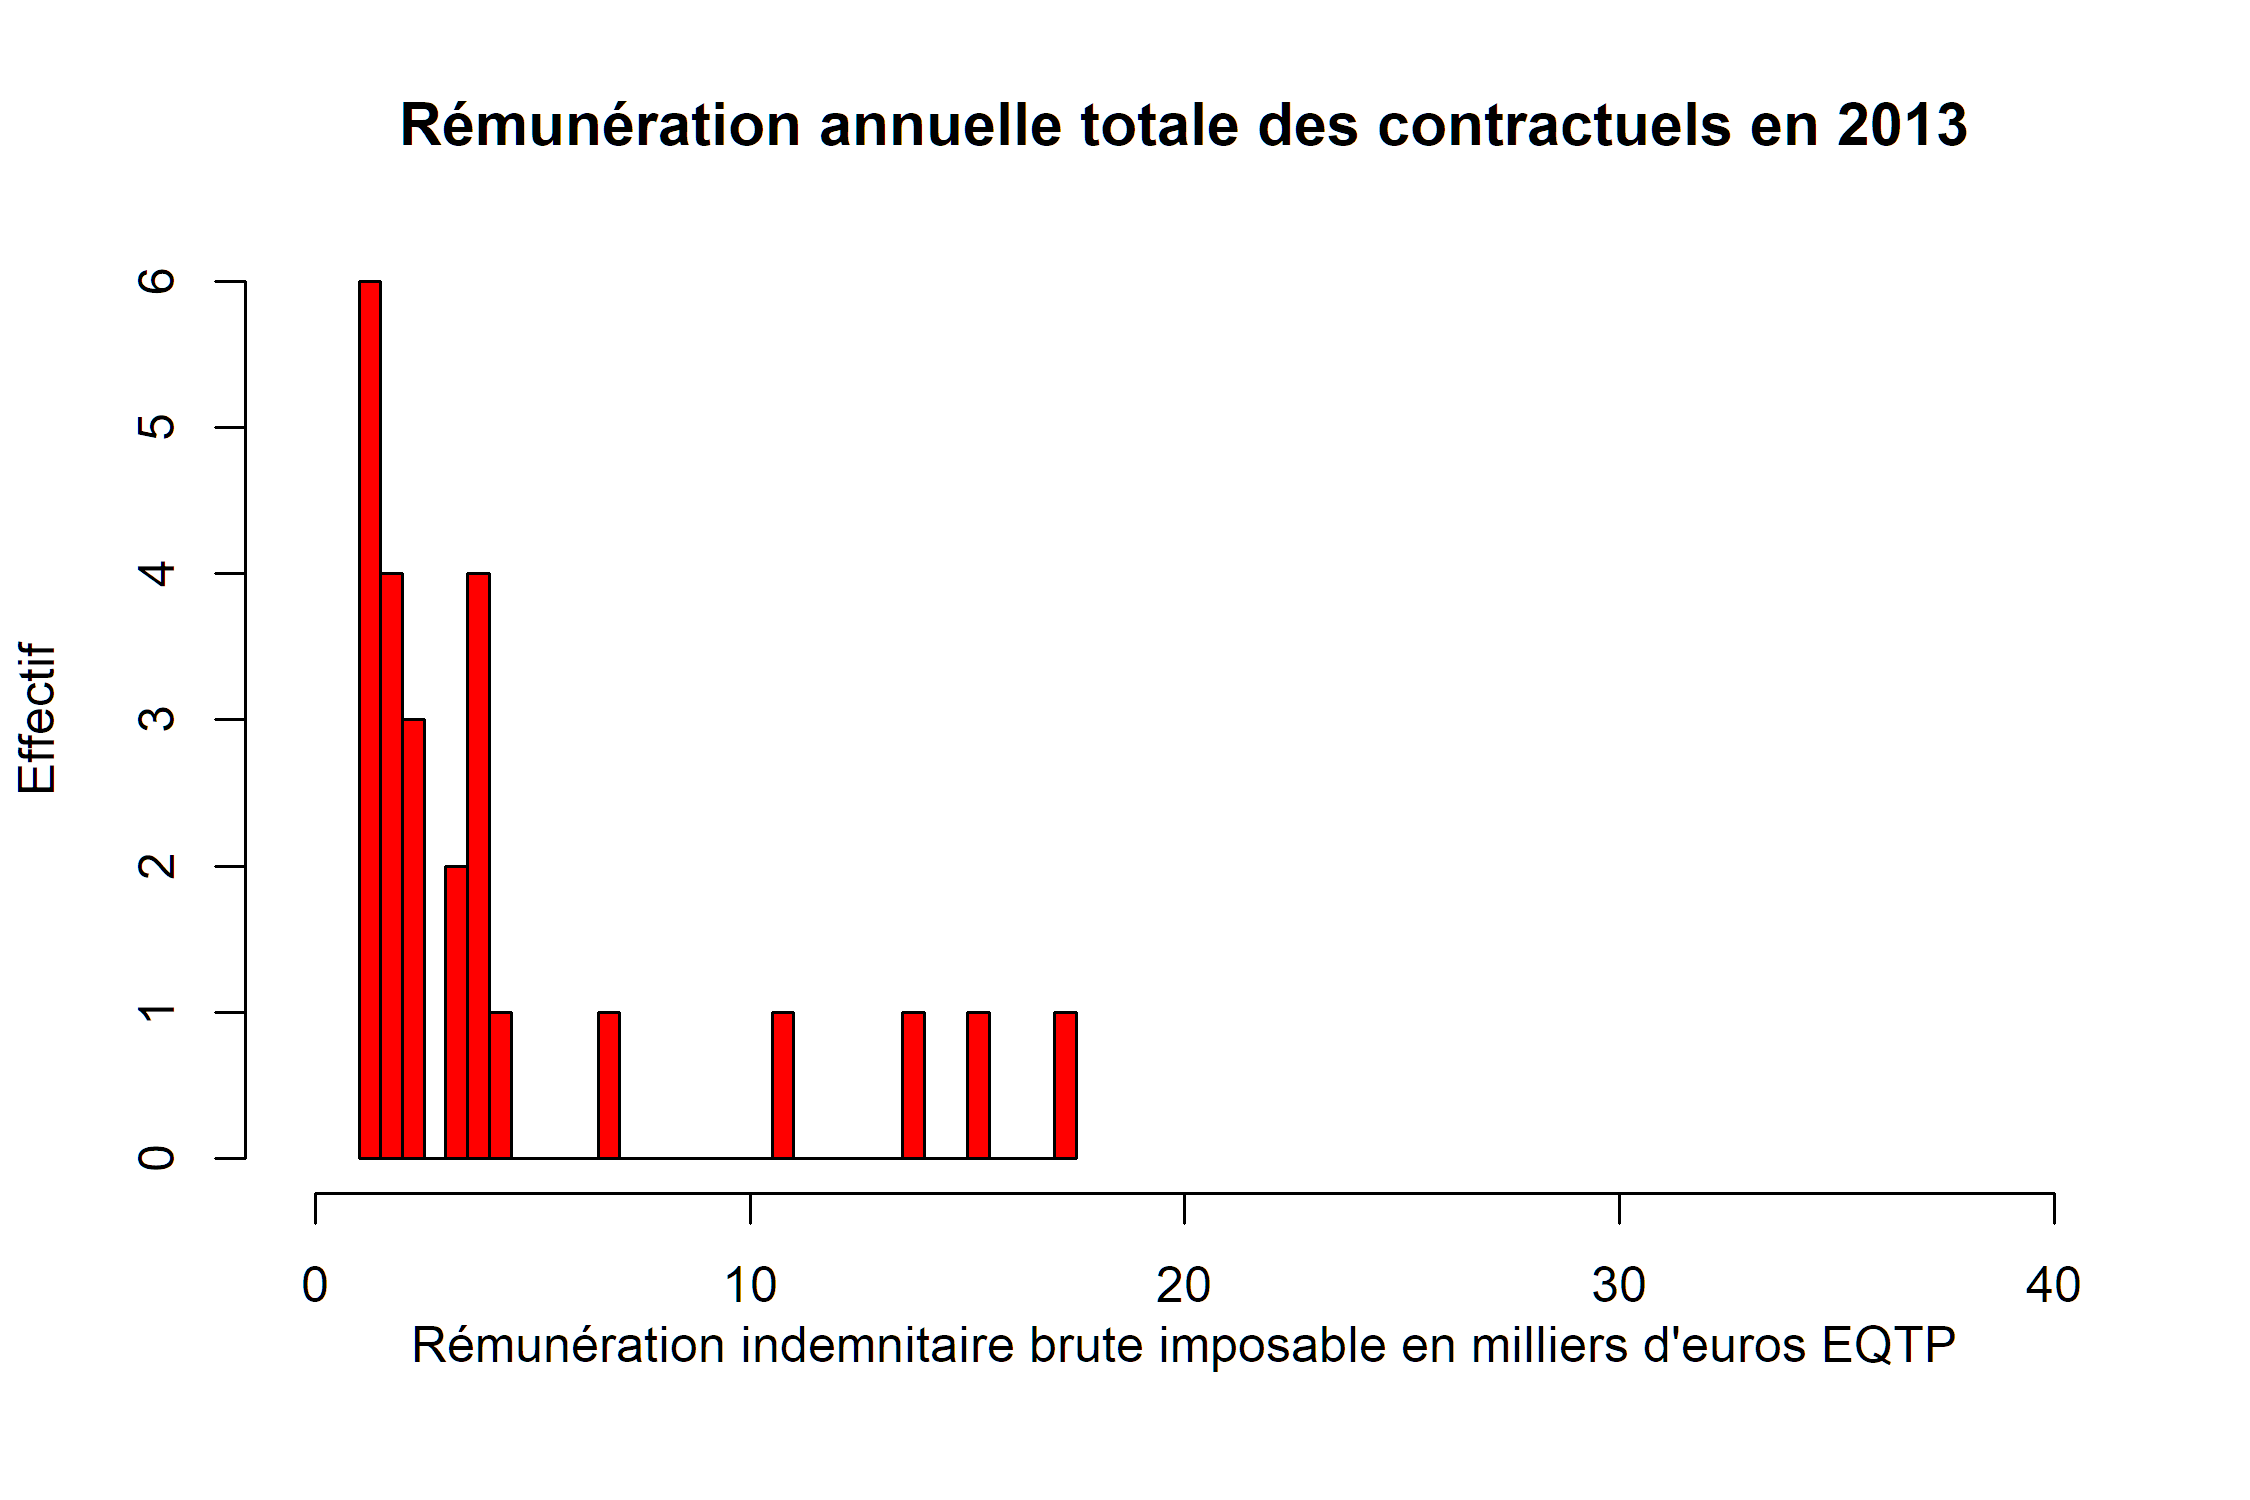
\includegraphics{altair_files/figure-latex/unnamed-chunk-94-1.png}

\textbf{Nota :} Ne sont retenues que les rémunérations supérieures à 1
000 k€. Les élus ne sont pas pris en compte.

\textbf{Formation et distribution du salaire brut moyen par tête (SMPT)
en EQTP pour l'année 2014 }

~\emph{Tableau 3.3.1}

\begin{longtable}[]{@{}rrrrr@{}}
\toprule
Statistique & Primes & Autres rémunérations & Quotité &
Effectif\tabularnewline
\midrule
\endhead
Minimum & -5 600 & 0 & 0,17 &\tabularnewline
1er quartile & 930 & 0 & 0,75 &\tabularnewline
Médiane & 2 060 & 0 & 1 &\tabularnewline
Moyenne & 2 500 & 0 & 0,86 & 356\tabularnewline
3ème quartile & 3 459 & 0 & 1 &\tabularnewline
Maximum & 15 113 & 0 & 1 &\tabularnewline
\bottomrule
\end{longtable}

~\emph{Tableau 3.3.2}

\begin{longtable}[]{@{}rrrrr@{}}
\toprule
Statistique & Total rémunérations & Total rémunérations EQTP & Quotité &
Effectif\tabularnewline
\midrule
\endhead
Minimum & 4 351 & 56 847 & 0,17 &\tabularnewline
1er quartile & 15 966 & 210 979 & 0,75 &\tabularnewline
Médiane & 21 518 & 256 476 & 1 &\tabularnewline
Moyenne & 32 560 & 395 316 & 0,86 & 356\tabularnewline
3ème quartile & 25 665 & 319 920 & 1 &\tabularnewline
Maximum & 131 280 & 1 545 714 & 1 &\tabularnewline
\bottomrule
\end{longtable}

\href{../Bases/Remunerations/Analyse.remunerations.csv}{Lien vers la base
des rémunérations}

\newpage

\hypertarget{remunerations-brutes-par-grade-et-par-emploi}{%
\subsection{3.4 Rémunérations brutes par grade et par
emploi}\label{remunerations-brutes-par-grade-et-par-emploi}}

\href{../Bases/Remunerations/brut.eqtp.csv}{Rémunérations brutes par grade}

\href{../Bases/Remunerations/brut.eqtp.emploi.csv}{Rémunérations brutes par
emploi}

\hypertarget{comparaisons-source-inseedgcl}{%
\subsection{3.5 Comparaisons source
INSEE/DGCL}\label{comparaisons-source-inseedgcl}}

\emph{Salaires annnuels bruts moyens 2011-2017 en EQTP (hors assistantes
maternelles)}

~\emph{Tableau 3.5.1}

\begin{longtable}[]{@{}llllllll@{}}
\toprule
Agrégat (euros) & 2011 & 2012 & 2013 & 2014 & 2015 & 2016 &
2017\tabularnewline
\midrule
\endhead
Ensemble & 25 908 & 26 340 & 26 616 & 26 844 & 27 384 & 27 636 & 28
356\tabularnewline
Titulaires & 26 676 & 27 108 & 27 444 & 28 044 & 28 464 & 28 764 & 29
472\tabularnewline
Autres salariés* & 22 836 & NA & 24 360 & 24 504 & 24 696 & 24 828 & 25
320\tabularnewline
\bottomrule
\end{longtable}

\begin{itemize}
\tightlist
\item
  \emph{Contractuels à partir de 2017} *
\end{itemize}

\textbf{Eléments de la rémunération brute pour les titulaires de la
fonction publique territoriale}

~\emph{Tableau 3.5.2}

\begin{longtable}[]{@{}lllllll@{}}
\toprule
Rém. annuelles & 2011 & Primes & 2012 & Primes & 2013 &
Primes\tabularnewline
\midrule
\endhead
Salaire brut & 26 660 & & 27 108 & & 27 444 &\tabularnewline
Traitement brut & 20 562 & 22,9 \% & 20 724 & 23,6 \% & 21 060 & 23,6
\%\tabularnewline
Primes et rémunérations annexes & & & & & &\tabularnewline
y compris IR et SFT & 6 098 & & 6 384 & & 6 384 &\tabularnewline
\bottomrule
\end{longtable}

\begin{longtable}[]{@{}lllllll@{}}
\toprule
Rém. annuelles & 2014 & Primes & 2015 & Primes & 2016 &
Primes\tabularnewline
\midrule
\endhead
Salaire brut & 28 044 & & 28 464 & & 28 764 &\tabularnewline
Traitement brut & 21 456 & 23,5 \% & 21 816 & 23,4 \% & 22 104 & 23,2
\%\tabularnewline
Primes et rémunérations annexes & & & & & &\tabularnewline
y compris IR et SFT & 6 588 & & 6 648 & & 6 660 &\tabularnewline
\bottomrule
\end{longtable}

\emph{Champ : France. Salariés en équivalent-temps plein (EQTP) des
collectivités territoriales (y compris bénéficiaires de contrats aidés,
hors assistantes maternelles).}\\
\emph{Les primes sont cumulées au supplément familial de traitement
(SFT) et à l'indemnité de résidence (IR). Le cumul est rapporté à la
rémunération brute totale.}\\
\href{../Docs/ip1486.xls}{Source INSEE}\\
\href{../Docs/Vue3_Remuneration_2017.xlsx}{Source DGCL}\\
\href{../Docs/Vue-Remunerations-2018.xlsx}{Source DGCL}\\
\href{../Docs/RA_2015.pdf}{Source RAEFP 2015}\\
\href{../Docs/RA_2016.pdf}{Source RAEFP 2016}\\
\href{../Docs/RA_2017.pdf}{Source RAEFP 2017}\\
\href{../Docs/RA_2018.pdf}{Source RAEFP 2018}

\hypertarget{cout-charge}{%
\subsection{3.6 Coût chargé}\label{cout-charge}}

\textbf{Les liens ci-après renvoient vers des tableaux présentant le
coût moyen chargé par agent}

\href{../Bases/Remunerations/cout.eqtp.csv}{Coût moyen chargé par grade}

\href{../Bases/Remunerations/cout.eqtp.emploi.csv}{Coût moyen chargé par
emploi}

\hypertarget{remunerations-nettes-evolutions-sur-la-periode-sous-revue}{%
\section{4. Rémunérations nettes : évolutions sur la periode sous
revue}\label{remunerations-nettes-evolutions-sur-la-periode-sous-revue}}

\textbf{Nombre d'exercices: 4 }

\textbf{Périmètre des données}\\
\textbf{Les données présentées dans cette section sont toutes relatives
à des rémunérations nettes en équivalent temps plein (EQTP)}\\
\textbf{Les élus, les vacataires et les assistantes maternelles ont été
retirés de la population étudiée}\\
\textbf{Seuls sont considérés les postes actifs et non annexes}

\emph{Nota :}\\
\emph{Rémunération annualisée en EQTP (Equivalent temps plein) : la
rémunération annuelle équivalente pour un temps plein en année pleine
est calculée pour chaque agent}\\
\emph{Chaque agent est rentre ensuite dans la somme avec la pondération
correspondant à son temps de travail annuel. }

\hypertarget{distribution-de-la-remuneration-nette-moyenne-sur-la-periode}{%
\subsection{4.1 Distribution de la rémunération nette moyenne sur la
periode}\label{distribution-de-la-remuneration-nette-moyenne-sur-la-periode}}

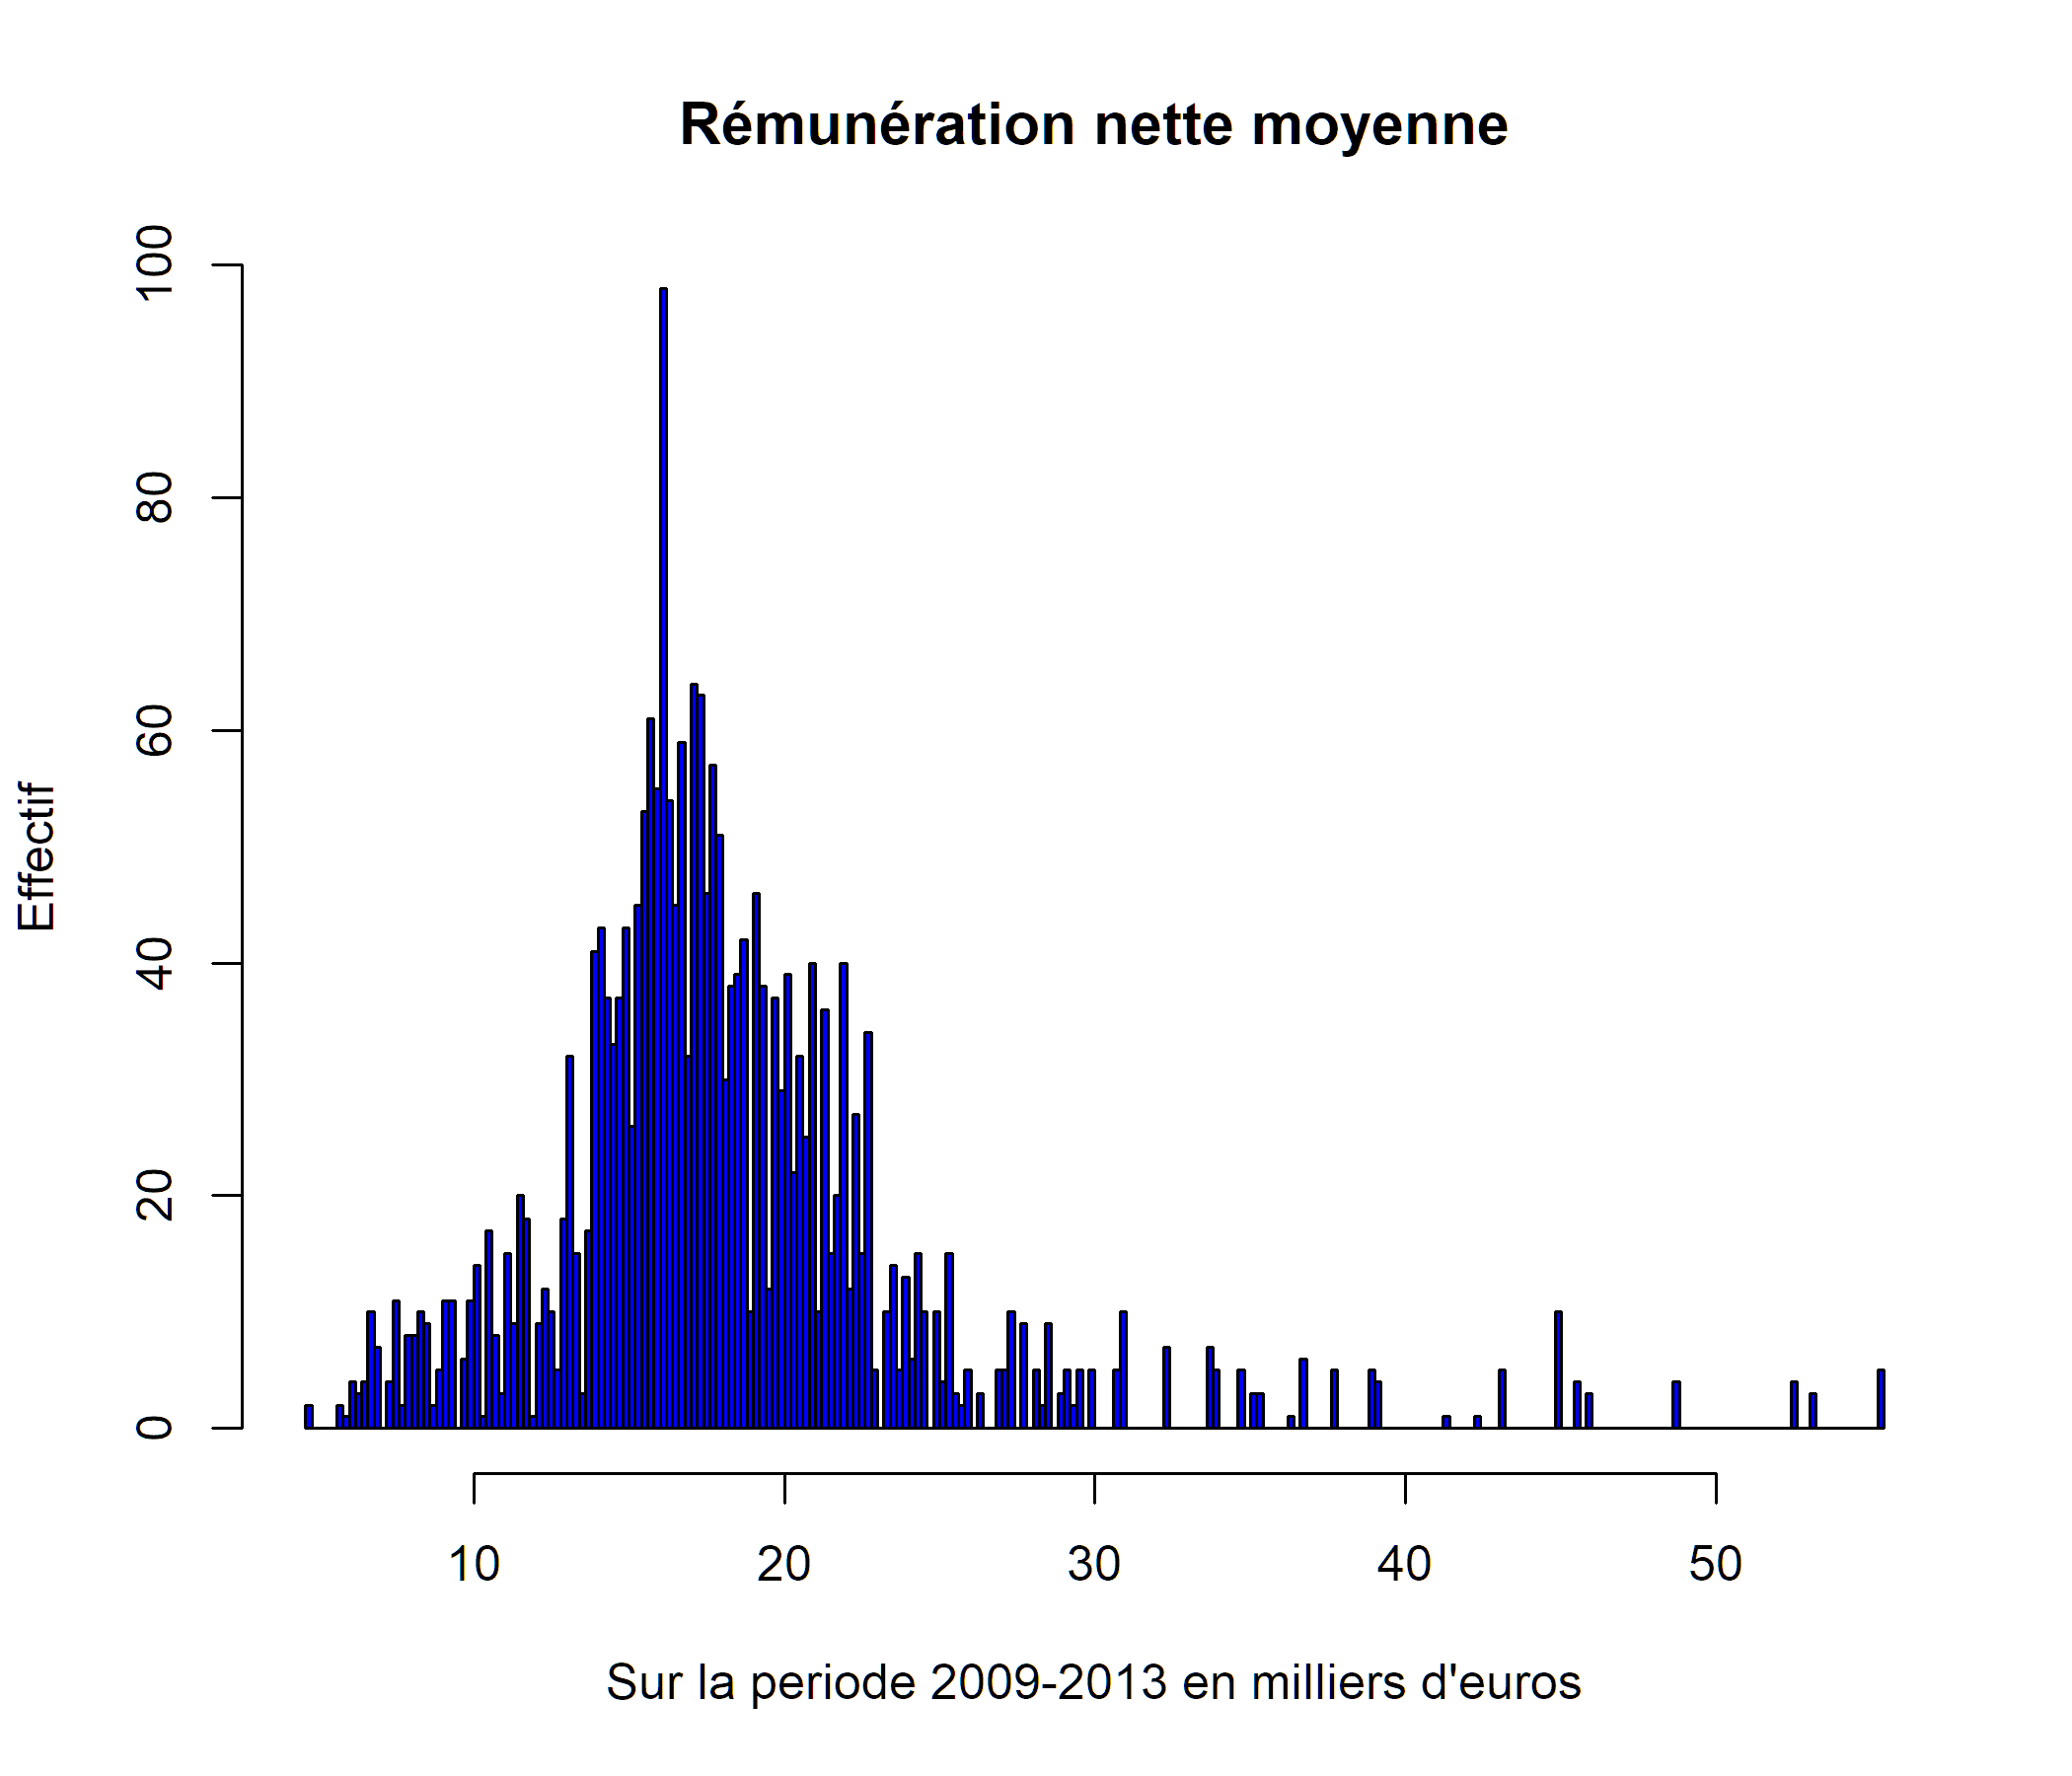
\includegraphics{altair_files/figure-latex/unnamed-chunk-115-1.png}

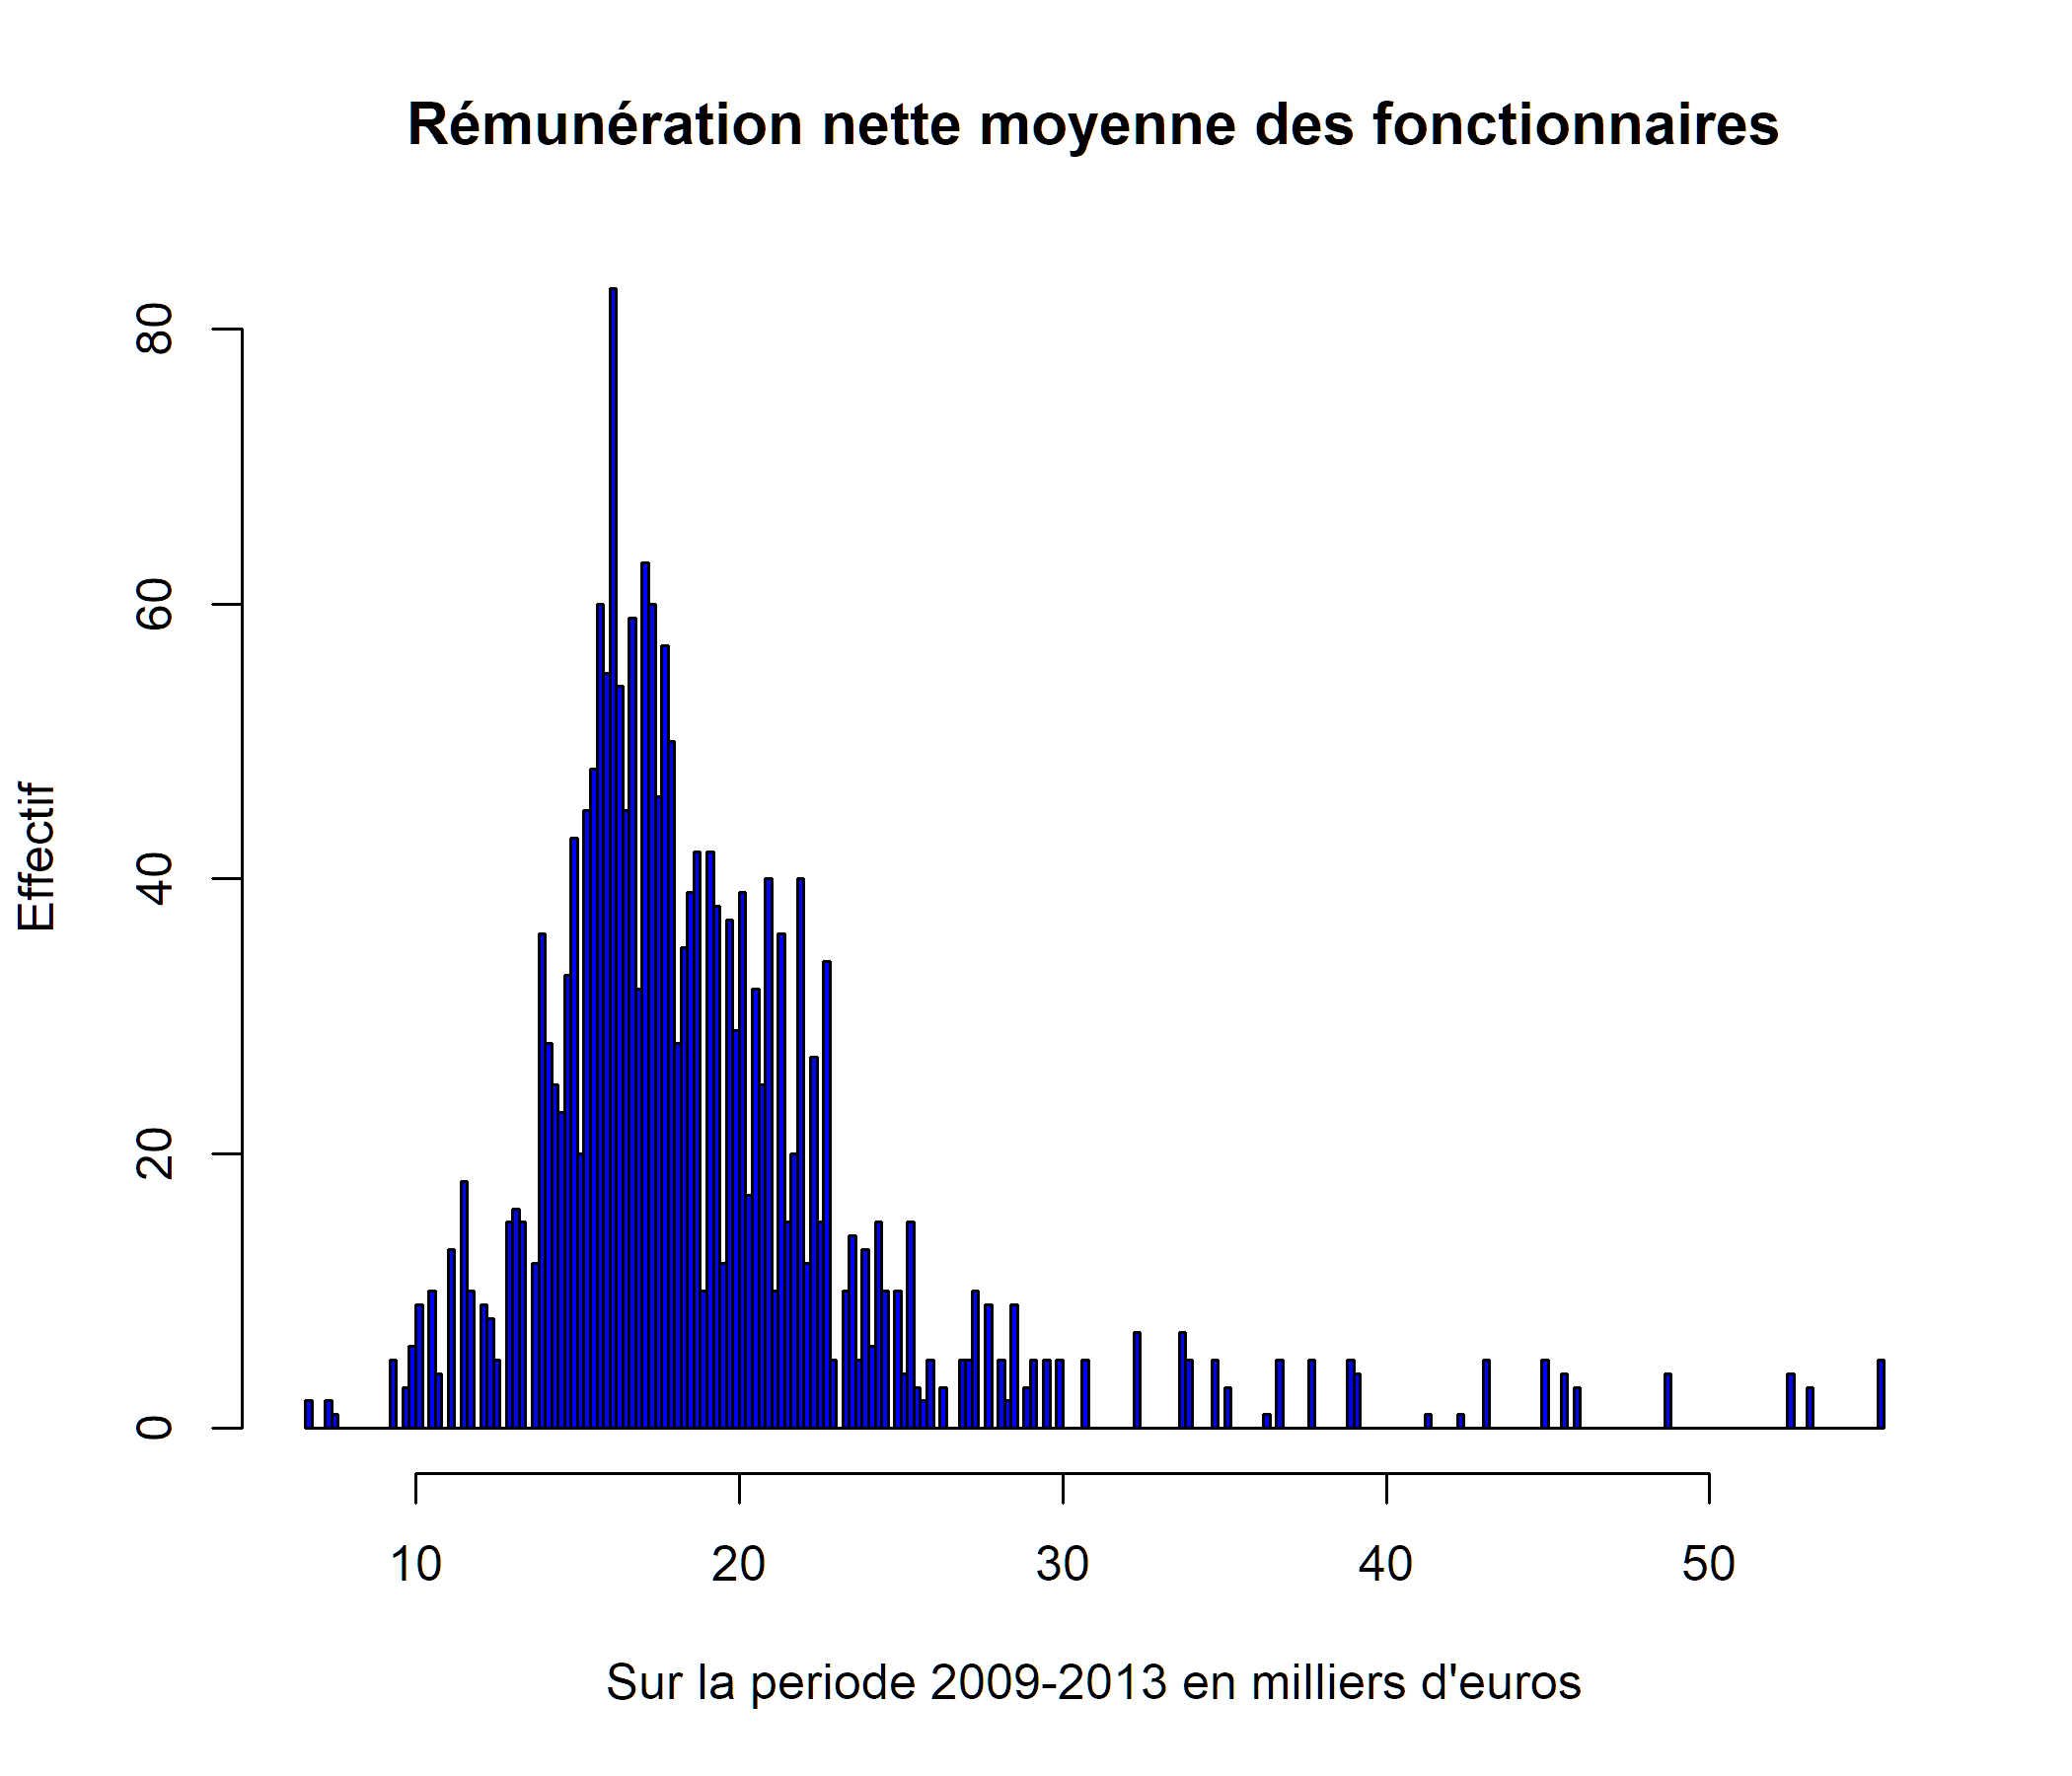
\includegraphics{altair_files/figure-latex/unnamed-chunk-116-1.png}

\href{../Bases/Remunerations/Analyse.variations.csv}{Lien vers la base de
données synthétique}\\
\href{../Bases/Remunerations/Analyse.variations.par.exercice.csv}{Lien vers
la base de données détaillée par année}

\hypertarget{evolutions-du-smpt-sur-la-periode-sous-revue}{%
\subsection{4.2 Evolutions du SMPT sur la periode sous
revue}\label{evolutions-du-smpt-sur-la-periode-sous-revue}}

\hypertarget{evolution-du-smpt-pour-lensemble-des-personnels-fonctionnaires-et-non-titulaires-hors-elus}{%
\subsubsection{4.2.1 Evolution du SMPT pour l'ensemble des personnels
fonctionnaires et non titulaires (hors
élus)}\label{evolution-du-smpt-pour-lensemble-des-personnels-fonctionnaires-et-non-titulaires-hors-elus}}

\textbf{Salaire net moyen par tête (SMPT net) en EQTP, hors élus}

~\emph{Tableau 4.2.1.1}

Il manque une ligne au moins dans la table. Annulation. {[}extra =
variation{]}\\
NULL

\textbf{Distribution et variation sur la periode du salaire moyen net
par tête (SMPT net) en EQTP}\\
\textbf{pour les salariés à temps complet}

~\emph{Tableau 4.2.1.2}

Table non générée.NULL

\emph{Nota :} La population retenue est constituée des agents qui ne
font pas partie des 2 centiles extrêmaux

Les élus, vacataires et assistantes maternelles sont retirés du
périmètre.\\
TC : personnels à temps complet sur toute l'annee\\
Seuls sont pris en compte les agents ayant connu au moins un mois actif
et ayant eu, sur l'annee, des rémunérations non annexes.\\
\href{../Docs/méthodologie.pdf}{Compléments méthodologiques}

\textbf{Comparaisons source INSEE/DGCL}

\textbf{Salaires nets annuels moyens en EQTP (hors assistantes
maternelles) dans la FPT}

~\emph{Tableau 4.2.1.3}

\begin{longtable}[]{@{}lrrrrrr@{}}
\toprule
net (euros) & 2011 & 2012 & 2013 & 2014 & 2016 & 2017\tabularnewline
\midrule
\endhead
Ensemble & 21 876 & 22 176 & 22 224 & 22 524 & 22 824 & 23
328\tabularnewline
Titulaires & 22 632 & 22 920 & 22 920 & 23 424 & 23 820 & 24
312\tabularnewline
Autres salariés* & 18 864 & NA & NA & 18 732 & 20 207 & 20
532\tabularnewline
\bottomrule
\end{longtable}

*Contractuels à partir de 2017

\emph{Champ : France. Salariés en équivalent-temps plein (EQTP) des
collectivités territoriales (y compris bénéficiaires de contrats aidés,
hors assistantes maternelles).}

\textbf{Distribution des salaires nets annuels en EQTP dans la fonction
publique territoriale (2011-2016)}

~\emph{Tableau 4.2.1.4}

\begin{longtable}[]{@{}llllll@{}}
\toprule
Décile ~euros & 2011 FPT & 2013 FPT & 2014 FPT & 2016 FPT & 2017
FPT\tabularnewline
\midrule
\endhead
D1 & 15 288 & 15 600 & 15 768 & 15 912 & 16 272\tabularnewline
D2 & 16 512 & 16 860 & 17 124 & 17 340 & 17 688\tabularnewline
D3 & 17 508 & 17 844 & 18 156 & 18 432 & 18 828\tabularnewline
D4 & 18 480 & 18 816 & 19 164 & 19 476 & 19 908\tabularnewline
D5 (médiane) & 19 632 & 19 908 & 20 256 & 20 616 & 21 096\tabularnewline
D6 & 21 012 & 21 300 & 21 648 & 22 020 & 22 548\tabularnewline
D7 & 22 860 & 23 160 & 23 496 & 23 868 & 24 444\tabularnewline
D8 & 25 596 & 25 956 & 26 292 & 26 700 & 27 336\tabularnewline
D9 & 30 876 & 31 272 & 31 596 & 31 968 & 32 652\tabularnewline
Moyenne & 21 876 & 22 212 & 22 524 & 22 824 & 23 328\tabularnewline
\bottomrule
\end{longtable}

\textbf{Distribution des salaires nets annuels en EQTP dans la fonction
publique d'Etat (2011-2016)}

~\emph{Tableau 4.2.1.5}

\begin{longtable}[]{@{}llll@{}}
\toprule
Décile ~euros & 2011 & 2013 & 2016\tabularnewline
\midrule
\endhead
D1 & 17 496 & 18 012 & 17 928\tabularnewline
D2 & 20 916 & 21 348 & 21 588\tabularnewline
D3 & 23 052 & 23 376 & 23 844\tabularnewline
D4 & 24 912 & 25 248 & 25 764\tabularnewline
D5 (médiane) & 26 832 & 27 120 & 27 720\tabularnewline
D6 & 28 944 & 29 220 & 29 760\tabularnewline
D7 & 31 632 & 31 968 & 32 604\tabularnewline
D8 & 35 592 & 35 964 & 36 588\tabularnewline
D9 & 42 456 & 42 780 & 43 332\tabularnewline
Moyenne & 29 208 & 29 628 & 30 060\tabularnewline
\bottomrule
\end{longtable}

\textbf{Distribution des salaires nets annuels en EQTP dans la fonction
publique hospitalière (hôpitaux) (2011-2016)}

~\emph{Tableau 4.2.1.6}

\begin{longtable}[]{@{}lllll@{}}
\toprule
Décile ~euros & 2011 & 2013 & 2016 & 2017\tabularnewline
\midrule
\endhead
D1 & 16 584 & 17 016 & 17 460 & 17 688\tabularnewline
D2 & 18 168 & 18 492 & 18 852 & 19 104\tabularnewline
D3 & 19 620 & 19 872 & 20 160 & 20 460\tabularnewline
D4 & 21 048 & 21 192 & 21 456 & 21 816\tabularnewline
D5 (médiane) & 22 596 & 22 656 & 22 848 & 23 220\tabularnewline
D6 & 24 504 & 24 516 & 24 540 & 24 888\tabularnewline
D7 & 27 216 & 27 252 & 27 108 & 27 408\tabularnewline
D8 & 30 996 & 31 176 & 31 092 & 31 404\tabularnewline
D9 & 37 812 & 38 100 & 38 064 & 38 388\tabularnewline
Moyenne & 26 496 & 26 916 & 27 096 & 27 456\tabularnewline
\bottomrule
\end{longtable}

\href{../Docs/ip1486.xls}{Source INSEE, onglets Figure3, F1web et F3web -
2011}\\
\href{../Docs/vue3_remunerations.xls}{Source INSEE, onglets F V3.1-2, F
V3.1-5 - 2013}\\
\href{../Docs/Vue-Remunerations-2018.xlsx}{Source INSEE, onglet v3-2, V3-5
2016}

\hypertarget{evolution-du-smpt-des-fonctionnaires}{%
\subsubsection{4.2.2 Evolution du SMPT des
fonctionnaires}\label{evolution-du-smpt-des-fonctionnaires}}

\hypertarget{toutes-categories-statutaires}{%
\subparagraph{4.2.2.1 Toutes categories
statutaires}\label{toutes-categories-statutaires}}

\textbf{Salaire net moyen par tête (SMPT net) en EQTP}

~\emph{Tableau 4.2.2.1.1}

Il manque une ligne au moins dans la table. Annulation. {[}extra =
variation{]}\\
NULL

\hypertarget{par-categorie-statutaire}{%
\subparagraph{4.2.2.2 Par categorie
statutaire}\label{par-categorie-statutaire}}

\textbf{Categorie A}

~\emph{Tableau 4.2.2.2.1}

Il manque une ligne au moins dans la table. Annulation. {[}extra =
variation{]}\\
NULL

\emph{Comparaisons nationales}\\
\emph{FPT categorie A}

\begin{longtable}[]{@{}lllll@{}}
\toprule
Décile ~euros & 2011 & 2013 & 2014 & 2016\tabularnewline
\midrule
\endhead
D1 & 26 040 & 26 340 & 26 460 & 26 724\tabularnewline
D2 & 28 992 & & &\tabularnewline
D3 & 31 272 & & &\tabularnewline
D4 & 33 468 & & &\tabularnewline
D5 (médiane) & 35 820 & 36 312 & 36 580 & 37 020\tabularnewline
D6 & 38 664 & & &\tabularnewline
D7 & 42 276 & & &\tabularnewline
D8 & 47 124 & & &\tabularnewline
D9 & 54 840 & 55 032 & 55 440 & 55 284\tabularnewline
Moyenne & 38 700 & 39 120 & 39 360 & 39 564\tabularnewline
\bottomrule
\end{longtable}

\textbf{Categorie B}

~\emph{Tableau 4.2.2.2.2}

Il manque une ligne au moins dans la table. Annulation. {[}extra =
variation{]}\\
NULL

\emph{Comparaisons nationales}\\
\emph{FPT categorie B}

\begin{longtable}[]{@{}lllll@{}}
\toprule
Décile ~euros & 2011 & 2013 & 2014 & 2016\tabularnewline
\midrule
\endhead
D1 & 20 580 & 20 964 & 21 108 & 21 372\tabularnewline
D2 & 22 272 & & &\tabularnewline
D3 & 23 652 & & &\tabularnewline
D4 & 24 960 & & &\tabularnewline
D5 (médiane) & 26 244 & 26 820 & 27 000 & 27 216\tabularnewline
D6 & 27 636 & & &\tabularnewline
D7 & 29 160 & & &\tabularnewline
D8 & 30 984 & & &\tabularnewline
D9 & 33 804 & 34 224 & 34 344 & 34 560\tabularnewline
Moyenne & 26 940 & 27 408 & 27 588 & 27 828\tabularnewline
\bottomrule
\end{longtable}

\textbf{Categorie C}

~\emph{Tableau 4.2.2.2.3}

Il manque une ligne au moins dans la table. Annulation. {[}extra =
variation{]}\\
NULL

\emph{Comparaisons nationales}\\
\emph{FPT categorie C}

\begin{longtable}[]{@{}lllll@{}}
\toprule
Décile ~euros & 2011 & 2013 & 2014 & 2016\tabularnewline
\midrule
\endhead
D1 & 15 972 & 16 296 & 16 632 & 16 920\tabularnewline
D2 & 16 896 & & &\tabularnewline
D3 & 17 652 & & &\tabularnewline
D4 & 18 360 & & &\tabularnewline
D5 (médiane) & 19 164 & 19 464 & 19 884 & 20 256\tabularnewline
D6 & 20 100 & & &\tabularnewline
D7 & 21 216 & & &\tabularnewline
D8 & 22 680 & & &\tabularnewline
D9 & 24 996 & 25 176 & 25 608 & 26 028\tabularnewline
Moyenne & 20 016 & 20 268 & 20 676 & 21 024\tabularnewline
\bottomrule
\end{longtable}

\hypertarget{distribution-et-variation-sur-la-periode-du-smpt-net-en-eqtp}{%
\subsubsection{4.2.3 Distribution et variation sur la periode du SMPT
net en
EQTP}\label{distribution-et-variation-sur-la-periode-du-smpt-net-en-eqtp}}

\hypertarget{pour-lensemble-des-categories-statutaires}{%
\paragraph{4.2.3.1 Pour l'ensemble des categories
statutaires}\label{pour-lensemble-des-categories-statutaires}}

\textbf{Fonctionnaires}\\
\hspace*{0.333em}\emph{Tableau 4.2.3.1.1}

Table non générée.NULL

\hypertarget{par-categorie-statutaire-1}{%
\paragraph{4.2.3.2 Par categorie
statutaire}\label{par-categorie-statutaire-1}}

\textbf{Categorie A}\\
\hspace*{0.333em}\emph{Tableau 4.2.3.2.1}

Table non générée.NULL

\textbf{Categorie B}\\
\hspace*{0.333em}\emph{Tableau 4.2.3.2.2}

Table non générée.NULL

\textbf{Categorie C}\\
\hspace*{0.333em}\emph{Tableau 4.2.3.2.3}

Table non générée.NULL

\href{../Bases/Remunerations/Analyse.variations.par.exercice.csv}{Lien vers
la base de données}

\hypertarget{remuneration-moyenne-des-personnes-en-place-rmpp-et-effet-de-noria}{%
\subsection{4.3 Rémunération moyenne des personnes en place (RMPP) et
effet de
noria}\label{remuneration-moyenne-des-personnes-en-place-rmpp-et-effet-de-noria}}

\hypertarget{rmpp-de-lensemble-des-personnels-titulaires-et-non-titulaires}{%
\subsubsection{4.3.1 RMPP de l'ensemble des personnels titulaires et
non-titulaires}\label{rmpp-de-lensemble-des-personnels-titulaires-et-non-titulaires}}

\hypertarget{application-de-filtres-sur-les-donnees}{%
\subsubsection{Application de filtres sur les
données}\label{application-de-filtres-sur-les-donnees}}

\textbf{Afin d'apprécier la sensibilité des résultats à la qualité ou
aux valeurs extrêmes des données, le filtrage suivant est à présent
appliqué.}\\
\textbf{Sont retirés les valeurs manquantes des variations, les centiles
extrêmaux, les rémunérations nettes négatives (rappels) ou proche de
zéro.}

\textbf{Un statut explicite doit être renseigné en fin de periode. Des
rémunérations doivent être versées à la fois en début et en fin de
periode de paiement de l'agent, supérieures à 0,5 . Le nombre de jours
d'exercice doit être supérieur à 4 .}

\textbf{Ces filtres sont référencés ci-après par les termes ``filtres
sur RMPP''.}

\emph{Cet histogramme décrit l'évolution de la rémunération moyenne des
personnes en place (RMPP), définies comme présentes deux annees entières
consécutives avec la même quotité}\\
\emph{L'évolution de la RMPP permet d'étudier le glissement
vieillesse-technicité ``positif'', à effectifs constants sur deux
années}

\textbf{Variation individuelle de rémunération nette en EQTP pour les
personnels présents sur toute la periode}

~\emph{Tableau 4.3.1.1}

\begin{longtable}[]{@{}rrrrr@{}}
\toprule
\begin{minipage}[b]{0.12\columnwidth}\raggedleft
Statistique\strut
\end{minipage} & \begin{minipage}[b]{0.22\columnwidth}\raggedleft
Variation normalisée (\%)\strut
\end{minipage} & \begin{minipage}[b]{0.37\columnwidth}\raggedleft
Variation annuelle moyenne normalisée (\%)\strut
\end{minipage} & \begin{minipage}[b]{0.07\columnwidth}\raggedleft
Quotité\strut
\end{minipage} & \begin{minipage}[b]{0.08\columnwidth}\raggedleft
Effectif\strut
\end{minipage}\tabularnewline
\midrule
\endhead
\begin{minipage}[t]{0.12\columnwidth}\raggedleft
Minimum\strut
\end{minipage} & \begin{minipage}[t]{0.22\columnwidth}\raggedleft
-56\strut
\end{minipage} & \begin{minipage}[t]{0.37\columnwidth}\raggedleft
-24\strut
\end{minipage} & \begin{minipage}[t]{0.07\columnwidth}\raggedleft
0,3\strut
\end{minipage} & \begin{minipage}[t]{0.08\columnwidth}\raggedleft
\strut
\end{minipage}\tabularnewline
\begin{minipage}[t]{0.12\columnwidth}\raggedleft
1er quartile\strut
\end{minipage} & \begin{minipage}[t]{0.22\columnwidth}\raggedleft
0,67\strut
\end{minipage} & \begin{minipage}[t]{0.37\columnwidth}\raggedleft
0,22\strut
\end{minipage} & \begin{minipage}[t]{0.07\columnwidth}\raggedleft
0,9\strut
\end{minipage} & \begin{minipage}[t]{0.08\columnwidth}\raggedleft
\strut
\end{minipage}\tabularnewline
\begin{minipage}[t]{0.12\columnwidth}\raggedleft
Médiane\strut
\end{minipage} & \begin{minipage}[t]{0.22\columnwidth}\raggedleft
5,6\strut
\end{minipage} & \begin{minipage}[t]{0.37\columnwidth}\raggedleft
1,8\strut
\end{minipage} & \begin{minipage}[t]{0.07\columnwidth}\raggedleft
1\strut
\end{minipage} & \begin{minipage}[t]{0.08\columnwidth}\raggedleft
\strut
\end{minipage}\tabularnewline
\begin{minipage}[t]{0.12\columnwidth}\raggedleft
Moyenne\strut
\end{minipage} & \begin{minipage}[t]{0.22\columnwidth}\raggedleft
6,1\strut
\end{minipage} & \begin{minipage}[t]{0.37\columnwidth}\raggedleft
1,7\strut
\end{minipage} & \begin{minipage}[t]{0.07\columnwidth}\raggedleft
0,94\strut
\end{minipage} & \begin{minipage}[t]{0.08\columnwidth}\raggedleft
716\strut
\end{minipage}\tabularnewline
\begin{minipage}[t]{0.12\columnwidth}\raggedleft
3ème quartile\strut
\end{minipage} & \begin{minipage}[t]{0.22\columnwidth}\raggedleft
12\strut
\end{minipage} & \begin{minipage}[t]{0.37\columnwidth}\raggedleft
3,7\strut
\end{minipage} & \begin{minipage}[t]{0.07\columnwidth}\raggedleft
1\strut
\end{minipage} & \begin{minipage}[t]{0.08\columnwidth}\raggedleft
\strut
\end{minipage}\tabularnewline
\begin{minipage}[t]{0.12\columnwidth}\raggedleft
Maximum\strut
\end{minipage} & \begin{minipage}[t]{0.22\columnwidth}\raggedleft
162\strut
\end{minipage} & \begin{minipage}[t]{0.37\columnwidth}\raggedleft
38\strut
\end{minipage} & \begin{minipage}[t]{0.07\columnwidth}\raggedleft
1\strut
\end{minipage} & \begin{minipage}[t]{0.08\columnwidth}\raggedleft
\strut
\end{minipage}\tabularnewline
\bottomrule
\end{longtable}

\hypertarget{rmpp-des-titulaires-et-stagiaires}{%
\subsubsection{4.3.2 RMPP des titulaires et
stagiaires}\label{rmpp-des-titulaires-et-stagiaires}}

\textbf{Variation individuelle de rémunération nette en EQTP pour les
personnels présents sur toute la periode}

~\emph{Tableau 4.3.2.1}

\begin{longtable}[]{@{}rrrrr@{}}
\toprule
\begin{minipage}[b]{0.12\columnwidth}\raggedleft
Statistique\strut
\end{minipage} & \begin{minipage}[b]{0.22\columnwidth}\raggedleft
Variation normalisée (\%)\strut
\end{minipage} & \begin{minipage}[b]{0.37\columnwidth}\raggedleft
Variation annuelle moyenne normalisée (\%)\strut
\end{minipage} & \begin{minipage}[b]{0.07\columnwidth}\raggedleft
Quotité\strut
\end{minipage} & \begin{minipage}[b]{0.08\columnwidth}\raggedleft
Effectif\strut
\end{minipage}\tabularnewline
\midrule
\endhead
\begin{minipage}[t]{0.12\columnwidth}\raggedleft
Minimum\strut
\end{minipage} & \begin{minipage}[t]{0.22\columnwidth}\raggedleft
-56\strut
\end{minipage} & \begin{minipage}[t]{0.37\columnwidth}\raggedleft
-24\strut
\end{minipage} & \begin{minipage}[t]{0.07\columnwidth}\raggedleft
0,46\strut
\end{minipage} & \begin{minipage}[t]{0.08\columnwidth}\raggedleft
\strut
\end{minipage}\tabularnewline
\begin{minipage}[t]{0.12\columnwidth}\raggedleft
1er quartile\strut
\end{minipage} & \begin{minipage}[t]{0.22\columnwidth}\raggedleft
0,55\strut
\end{minipage} & \begin{minipage}[t]{0.37\columnwidth}\raggedleft
0,18\strut
\end{minipage} & \begin{minipage}[t]{0.07\columnwidth}\raggedleft
0,89\strut
\end{minipage} & \begin{minipage}[t]{0.08\columnwidth}\raggedleft
\strut
\end{minipage}\tabularnewline
\begin{minipage}[t]{0.12\columnwidth}\raggedleft
Médiane\strut
\end{minipage} & \begin{minipage}[t]{0.22\columnwidth}\raggedleft
5,5\strut
\end{minipage} & \begin{minipage}[t]{0.37\columnwidth}\raggedleft
1,8\strut
\end{minipage} & \begin{minipage}[t]{0.07\columnwidth}\raggedleft
1\strut
\end{minipage} & \begin{minipage}[t]{0.08\columnwidth}\raggedleft
\strut
\end{minipage}\tabularnewline
\begin{minipage}[t]{0.12\columnwidth}\raggedleft
Moyenne\strut
\end{minipage} & \begin{minipage}[t]{0.22\columnwidth}\raggedleft
5,3\strut
\end{minipage} & \begin{minipage}[t]{0.37\columnwidth}\raggedleft
1,5\strut
\end{minipage} & \begin{minipage}[t]{0.07\columnwidth}\raggedleft
0,94\strut
\end{minipage} & \begin{minipage}[t]{0.08\columnwidth}\raggedleft
584\strut
\end{minipage}\tabularnewline
\begin{minipage}[t]{0.12\columnwidth}\raggedleft
3ème quartile\strut
\end{minipage} & \begin{minipage}[t]{0.22\columnwidth}\raggedleft
11\strut
\end{minipage} & \begin{minipage}[t]{0.37\columnwidth}\raggedleft
3,5\strut
\end{minipage} & \begin{minipage}[t]{0.07\columnwidth}\raggedleft
1\strut
\end{minipage} & \begin{minipage}[t]{0.08\columnwidth}\raggedleft
\strut
\end{minipage}\tabularnewline
\begin{minipage}[t]{0.12\columnwidth}\raggedleft
Maximum\strut
\end{minipage} & \begin{minipage}[t]{0.22\columnwidth}\raggedleft
157\strut
\end{minipage} & \begin{minipage}[t]{0.37\columnwidth}\raggedleft
37\strut
\end{minipage} & \begin{minipage}[t]{0.07\columnwidth}\raggedleft
1\strut
\end{minipage} & \begin{minipage}[t]{0.08\columnwidth}\raggedleft
\strut
\end{minipage}\tabularnewline
\bottomrule
\end{longtable}

\href{../Bases/Remunerations/Anavar.synthese.csv}{Lien vers la base de
données}

\textbf{Nota}

\emph{Personnes en place :} en fonction au moins deux années
consécutives avec la même quotité sur la periode 2011 à 2014

\emph{Variation sur la periode d'activité :} entre l'arrivée et le
départ de la personne\\
\emph{Variation normalisée :} conforme à la définition INSEE (présente
en début et en fin de période avec la même quotité)

\textbf{Commentaire}

Les différences éventuelles constatées entre l'évolution de la RMPP au
tableau -2 sont dues soit à l'effet de noria soit à l'effet périmètre.

\hypertarget{les-filtres-rmpp-appliques-au-4.3.1-et-4.3.2-ne-sont-plus-appliques.-il-peut-en-resulter-des-variations-significativement-differentes-de-celles-calculees-precedemment.}{%
\subparagraph{Les filtres RMPP appliqués au 4.3.1 et 4.3.2 ne sont plus
appliqués. Il peut en résulter des variations significativement
différentes de celles calculees
précédemment.}\label{les-filtres-rmpp-appliques-au-4.3.1-et-4.3.2-ne-sont-plus-appliques.-il-peut-en-resulter-des-variations-significativement-differentes-de-celles-calculees-precedemment.}}

\hypertarget{effet-de-noria-et-de-variation-deffectifs-sur-remunerations-moyennes}{%
\subsubsection{4.3.3 Effet de noria et de variation d'effectifs sur
rémunérations
moyennes}\label{effet-de-noria-et-de-variation-deffectifs-sur-remunerations-moyennes}}

\emph{Les calculs de RMPP sur la première année de la periode sous revue
sont estimatifs et ne devraient pas être pris en compte pour
publication.}

\textbf{Effet de noria et de variations d'effectifs sur rémunérations
nettes moyennes EQTP}

~\emph{Tableau 4.3.3.1}

\begin{longtable}[]{@{}lllllllll@{}}
\toprule
\begin{minipage}[b]{0.05\columnwidth}\raggedright
Annee\strut
\end{minipage} & \begin{minipage}[b]{0.08\columnwidth}\raggedright
Effectifs\strut
\end{minipage} & \begin{minipage}[b]{0.05\columnwidth}\raggedright
ETPT\strut
\end{minipage} & \begin{minipage}[b]{0.10\columnwidth}\raggedright
ETPT entrants\strut
\end{minipage} & \begin{minipage}[b]{0.10\columnwidth}\raggedright
ETPT sortants\strut
\end{minipage} & \begin{minipage}[b]{0.07\columnwidth}\raggedright
Entrants\strut
\end{minipage} & \begin{minipage}[b]{0.07\columnwidth}\raggedright
Sortants\strut
\end{minipage} & \begin{minipage}[b]{0.11\columnwidth}\raggedright
Var. effectifs\strut
\end{minipage} & \begin{minipage}[b]{0.14\columnwidth}\raggedright
Taux de rotation \%\strut
\end{minipage}\tabularnewline
\midrule
\endhead
\begin{minipage}[t]{0.05\columnwidth}\raggedright
2011\strut
\end{minipage} & \begin{minipage}[t]{0.08\columnwidth}\raggedright
825,0\strut
\end{minipage} & \begin{minipage}[t]{0.05\columnwidth}\raggedright
787,8\strut
\end{minipage} & \begin{minipage}[t]{0.10\columnwidth}\raggedright
43,9\strut
\end{minipage} & \begin{minipage}[t]{0.10\columnwidth}\raggedright
44,9\strut
\end{minipage} & \begin{minipage}[t]{0.07\columnwidth}\raggedright
87,0\strut
\end{minipage} & \begin{minipage}[t]{0.07\columnwidth}\raggedright
84,0\strut
\end{minipage} & \begin{minipage}[t]{0.11\columnwidth}\raggedright
3,0\strut
\end{minipage} & \begin{minipage}[t]{0.14\columnwidth}\raggedright
10,4\strut
\end{minipage}\tabularnewline
\begin{minipage}[t]{0.05\columnwidth}\raggedright
2012\strut
\end{minipage} & \begin{minipage}[t]{0.08\columnwidth}\raggedright
833,0\strut
\end{minipage} & \begin{minipage}[t]{0.05\columnwidth}\raggedright
808,3\strut
\end{minipage} & \begin{minipage}[t]{0.10\columnwidth}\raggedright
59,4\strut
\end{minipage} & \begin{minipage}[t]{0.10\columnwidth}\raggedright
50,0\strut
\end{minipage} & \begin{minipage}[t]{0.07\columnwidth}\raggedright
125,0\strut
\end{minipage} & \begin{minipage}[t]{0.07\columnwidth}\raggedright
96,0\strut
\end{minipage} & \begin{minipage}[t]{0.11\columnwidth}\raggedright
29,0\strut
\end{minipage} & \begin{minipage}[t]{0.14\columnwidth}\raggedright
13,3\strut
\end{minipage}\tabularnewline
\begin{minipage}[t]{0.05\columnwidth}\raggedright
2013\strut
\end{minipage} & \begin{minipage}[t]{0.08\columnwidth}\raggedright
853,0\strut
\end{minipage} & \begin{minipage}[t]{0.05\columnwidth}\raggedright
825,4\strut
\end{minipage} & \begin{minipage}[t]{0.10\columnwidth}\raggedright
55,5\strut
\end{minipage} & \begin{minipage}[t]{0.10\columnwidth}\raggedright
43,9\strut
\end{minipage} & \begin{minipage}[t]{0.07\columnwidth}\raggedright
103,0\strut
\end{minipage} & \begin{minipage}[t]{0.07\columnwidth}\raggedright
89,0\strut
\end{minipage} & \begin{minipage}[t]{0.11\columnwidth}\raggedright
14,0\strut
\end{minipage} & \begin{minipage}[t]{0.14\columnwidth}\raggedright
11,3\strut
\end{minipage}\tabularnewline
\begin{minipage}[t]{0.05\columnwidth}\raggedright
2014\strut
\end{minipage} & \begin{minipage}[t]{0.08\columnwidth}\raggedright
873,0\strut
\end{minipage} & \begin{minipage}[t]{0.05\columnwidth}\raggedright
824,2\strut
\end{minipage} & \begin{minipage}[t]{0.10\columnwidth}\raggedright
37,3\strut
\end{minipage} & \begin{minipage}[t]{0.10\columnwidth}\raggedright
47,1\strut
\end{minipage} & \begin{minipage}[t]{0.07\columnwidth}\raggedright
89,0\strut
\end{minipage} & \begin{minipage}[t]{0.07\columnwidth}\raggedright
88,0\strut
\end{minipage} & \begin{minipage}[t]{0.11\columnwidth}\raggedright
1,0\strut
\end{minipage} & \begin{minipage}[t]{0.14\columnwidth}\raggedright
10,1\strut
\end{minipage}\tabularnewline
\begin{minipage}[t]{0.05\columnwidth}\raggedright
Total\strut
\end{minipage} & \begin{minipage}[t]{0.08\columnwidth}\raggedright
\strut
\end{minipage} & \begin{minipage}[t]{0.05\columnwidth}\raggedright
\strut
\end{minipage} & \begin{minipage}[t]{0.10\columnwidth}\raggedright
196,1\strut
\end{minipage} & \begin{minipage}[t]{0.10\columnwidth}\raggedright
185,9\strut
\end{minipage} & \begin{minipage}[t]{0.07\columnwidth}\raggedright
404,0\strut
\end{minipage} & \begin{minipage}[t]{0.07\columnwidth}\raggedright
357,0\strut
\end{minipage} & \begin{minipage}[t]{0.11\columnwidth}\raggedright
47,0\strut
\end{minipage} & \begin{minipage}[t]{0.14\columnwidth}\raggedright
\strut
\end{minipage}\tabularnewline
\bottomrule
\end{longtable}

\begin{longtable}[]{@{}lllllllll@{}}
\toprule
\begin{minipage}[b]{0.05\columnwidth}\raggedright
Annee\strut
\end{minipage} & \begin{minipage}[b]{0.10\columnwidth}\raggedright
Effet noria\strut
\end{minipage} & \begin{minipage}[b]{0.06\columnwidth}\raggedright
\% SMPT\strut
\end{minipage} & \begin{minipage}[b]{0.16\columnwidth}\raggedright
Effet var. effectifs\strut
\end{minipage} & \begin{minipage}[b]{0.06\columnwidth}\raggedright
\% SMPT\strut
\end{minipage} & \begin{minipage}[b]{0.12\columnwidth}\raggedright
Effet vacances\strut
\end{minipage} & \begin{minipage}[b]{0.06\columnwidth}\raggedright
\% SMPT\strut
\end{minipage} & \begin{minipage}[b]{0.10\columnwidth}\raggedright
Total\strut
\end{minipage} & \begin{minipage}[b]{0.06\columnwidth}\raggedright
\% SMPT\strut
\end{minipage}\tabularnewline
\midrule
\endhead
\begin{minipage}[t]{0.05\columnwidth}\raggedright
2011\strut
\end{minipage} & \begin{minipage}[t]{0.10\columnwidth}\raggedright
181 485,9\strut
\end{minipage} & \begin{minipage}[t]{0.06\columnwidth}\raggedright
0,1\strut
\end{minipage} & \begin{minipage}[t]{0.16\columnwidth}\raggedright
272 742,3\strut
\end{minipage} & \begin{minipage}[t]{0.06\columnwidth}\raggedright
0,1\strut
\end{minipage} & \begin{minipage}[t]{0.12\columnwidth}\raggedright
601 524,7\strut
\end{minipage} & \begin{minipage}[t]{0.06\columnwidth}\raggedright
0,3\strut
\end{minipage} & \begin{minipage}[t]{0.10\columnwidth}\raggedright
1 055 752,9\strut
\end{minipage} & \begin{minipage}[t]{0.06\columnwidth}\raggedright
0,5\strut
\end{minipage}\tabularnewline
\begin{minipage}[t]{0.05\columnwidth}\raggedright
2012\strut
\end{minipage} & \begin{minipage}[t]{0.10\columnwidth}\raggedright
-1 473 886,8\strut
\end{minipage} & \begin{minipage}[t]{0.06\columnwidth}\raggedright
-0,6\strut
\end{minipage} & \begin{minipage}[t]{0.16\columnwidth}\raggedright
1 789 542,1\strut
\end{minipage} & \begin{minipage}[t]{0.06\columnwidth}\raggedright
0,8\strut
\end{minipage} & \begin{minipage}[t]{0.12\columnwidth}\raggedright
-50 066,3\strut
\end{minipage} & \begin{minipage}[t]{0.06\columnwidth}\raggedright
-0,0\strut
\end{minipage} & \begin{minipage}[t]{0.10\columnwidth}\raggedright
265 589,0\strut
\end{minipage} & \begin{minipage}[t]{0.06\columnwidth}\raggedright
0,1\strut
\end{minipage}\tabularnewline
\begin{minipage}[t]{0.05\columnwidth}\raggedright
2013\strut
\end{minipage} & \begin{minipage}[t]{0.10\columnwidth}\raggedright
1 683 365,1\strut
\end{minipage} & \begin{minipage}[t]{0.06\columnwidth}\raggedright
0,7\strut
\end{minipage} & \begin{minipage}[t]{0.16\columnwidth}\raggedright
1 273 144,9\strut
\end{minipage} & \begin{minipage}[t]{0.06\columnwidth}\raggedright
0,5\strut
\end{minipage} & \begin{minipage}[t]{0.12\columnwidth}\raggedright
481 855,1\strut
\end{minipage} & \begin{minipage}[t]{0.06\columnwidth}\raggedright
0,2\strut
\end{minipage} & \begin{minipage}[t]{0.10\columnwidth}\raggedright
3 438 365,1\strut
\end{minipage} & \begin{minipage}[t]{0.06\columnwidth}\raggedright
1,4\strut
\end{minipage}\tabularnewline
\begin{minipage}[t]{0.05\columnwidth}\raggedright
2014\strut
\end{minipage} & \begin{minipage}[t]{0.10\columnwidth}\raggedright
-1 429 847,3\strut
\end{minipage} & \begin{minipage}[t]{0.06\columnwidth}\raggedright
-0,6\strut
\end{minipage} & \begin{minipage}[t]{0.16\columnwidth}\raggedright
53 308,1\strut
\end{minipage} & \begin{minipage}[t]{0.06\columnwidth}\raggedright
0,0\strut
\end{minipage} & \begin{minipage}[t]{0.12\columnwidth}\raggedright
-514 859,9\strut
\end{minipage} & \begin{minipage}[t]{0.06\columnwidth}\raggedright
-0,2\strut
\end{minipage} & \begin{minipage}[t]{0.10\columnwidth}\raggedright
-1 891 399,1\strut
\end{minipage} & \begin{minipage}[t]{0.06\columnwidth}\raggedright
-0,8\strut
\end{minipage}\tabularnewline
\begin{minipage}[t]{0.05\columnwidth}\raggedright
Total\strut
\end{minipage} & \begin{minipage}[t]{0.10\columnwidth}\raggedright
-1 038 883,1\strut
\end{minipage} & \begin{minipage}[t]{0.06\columnwidth}\raggedright
\strut
\end{minipage} & \begin{minipage}[t]{0.16\columnwidth}\raggedright
3 388 737,5\strut
\end{minipage} & \begin{minipage}[t]{0.06\columnwidth}\raggedright
\strut
\end{minipage} & \begin{minipage}[t]{0.12\columnwidth}\raggedright
518 453,7\strut
\end{minipage} & \begin{minipage}[t]{0.06\columnwidth}\raggedright
\strut
\end{minipage} & \begin{minipage}[t]{0.10\columnwidth}\raggedright
2 868 308,0\strut
\end{minipage} & \begin{minipage}[t]{0.06\columnwidth}\raggedright
\strut
\end{minipage}\tabularnewline
\bottomrule
\end{longtable}

\begin{longtable}[]{@{}lllllllll@{}}
\toprule
Annee & RMPP & Entrées n - 1 & Noria & Var. effectifs & Vacances & Total
E/S & Ajustement & SMPT\tabularnewline
\midrule
\endhead
2011 & 309 599,4 & -0,1 & 0,1 & 0,1 & 0,2 & 0,3 & -0,05 & 296
540,4\tabularnewline
2012 & 316 323,1 & -0,5 & -0,6 & 0,7 & -0,0 & -0,4 & -0,06 & 294
867,0\tabularnewline
2013 & 323 828,7 & -2,9 & 0,6 & 0,5 & 0,2 & -1,7 & -0,06 & 298
900,4\tabularnewline
2014 & 318 917,9 & -0,6 & -0,5 & 0,0 & -0,2 & -1,3 & -0,04 & 301
906,4\tabularnewline
Moyenne géom. & 317 125,6 & -1,0 & -0,1 & 0,3 & 0,1 & -0,7 & -0,06 & 298
041,8\tabularnewline
\bottomrule
\end{longtable}

\begin{longtable}[]{@{}lllll@{}}
\toprule
Annee & Var. RMPP & Var. effets E/S & Cumul & Var. SMPT\tabularnewline
\midrule
\endhead
2011-2012 & 2,2 & -2,7 & -0,6 & -0,6\tabularnewline
2012-2013 & 2,4 & -1,0 & 1,4 & 1,4\tabularnewline
2013-2014 & -1,5 & 2,6 & 1,0 & 1,0\tabularnewline
2011-2014 & 3,0 & -1,2 & 1,8 & 1,8\tabularnewline
\bottomrule
\end{longtable}

\textbf{Effet de noria et de variations d'effectifs sur rémunérations
brutes moyennes EQTP}

~\emph{Tableau 4.3.3.2}

\begin{longtable}[]{@{}lllllllll@{}}
\toprule
\begin{minipage}[b]{0.05\columnwidth}\raggedright
Annee\strut
\end{minipage} & \begin{minipage}[b]{0.08\columnwidth}\raggedright
Effectifs\strut
\end{minipage} & \begin{minipage}[b]{0.05\columnwidth}\raggedright
ETPT\strut
\end{minipage} & \begin{minipage}[b]{0.10\columnwidth}\raggedright
ETPT entrants\strut
\end{minipage} & \begin{minipage}[b]{0.10\columnwidth}\raggedright
ETPT sortants\strut
\end{minipage} & \begin{minipage}[b]{0.07\columnwidth}\raggedright
Entrants\strut
\end{minipage} & \begin{minipage}[b]{0.07\columnwidth}\raggedright
Sortants\strut
\end{minipage} & \begin{minipage}[b]{0.11\columnwidth}\raggedright
Var. effectifs\strut
\end{minipage} & \begin{minipage}[b]{0.14\columnwidth}\raggedright
Taux de rotation \%\strut
\end{minipage}\tabularnewline
\midrule
\endhead
\begin{minipage}[t]{0.05\columnwidth}\raggedright
2011\strut
\end{minipage} & \begin{minipage}[t]{0.08\columnwidth}\raggedright
825,0\strut
\end{minipage} & \begin{minipage}[t]{0.05\columnwidth}\raggedright
787,8\strut
\end{minipage} & \begin{minipage}[t]{0.10\columnwidth}\raggedright
43,9\strut
\end{minipage} & \begin{minipage}[t]{0.10\columnwidth}\raggedright
44,9\strut
\end{minipage} & \begin{minipage}[t]{0.07\columnwidth}\raggedright
87,0\strut
\end{minipage} & \begin{minipage}[t]{0.07\columnwidth}\raggedright
84,0\strut
\end{minipage} & \begin{minipage}[t]{0.11\columnwidth}\raggedright
3,0\strut
\end{minipage} & \begin{minipage}[t]{0.14\columnwidth}\raggedright
10,4\strut
\end{minipage}\tabularnewline
\begin{minipage}[t]{0.05\columnwidth}\raggedright
2012\strut
\end{minipage} & \begin{minipage}[t]{0.08\columnwidth}\raggedright
833,0\strut
\end{minipage} & \begin{minipage}[t]{0.05\columnwidth}\raggedright
808,3\strut
\end{minipage} & \begin{minipage}[t]{0.10\columnwidth}\raggedright
59,4\strut
\end{minipage} & \begin{minipage}[t]{0.10\columnwidth}\raggedright
50,0\strut
\end{minipage} & \begin{minipage}[t]{0.07\columnwidth}\raggedright
125,0\strut
\end{minipage} & \begin{minipage}[t]{0.07\columnwidth}\raggedright
96,0\strut
\end{minipage} & \begin{minipage}[t]{0.11\columnwidth}\raggedright
29,0\strut
\end{minipage} & \begin{minipage}[t]{0.14\columnwidth}\raggedright
13,3\strut
\end{minipage}\tabularnewline
\begin{minipage}[t]{0.05\columnwidth}\raggedright
2013\strut
\end{minipage} & \begin{minipage}[t]{0.08\columnwidth}\raggedright
853,0\strut
\end{minipage} & \begin{minipage}[t]{0.05\columnwidth}\raggedright
825,4\strut
\end{minipage} & \begin{minipage}[t]{0.10\columnwidth}\raggedright
55,5\strut
\end{minipage} & \begin{minipage}[t]{0.10\columnwidth}\raggedright
43,9\strut
\end{minipage} & \begin{minipage}[t]{0.07\columnwidth}\raggedright
103,0\strut
\end{minipage} & \begin{minipage}[t]{0.07\columnwidth}\raggedright
89,0\strut
\end{minipage} & \begin{minipage}[t]{0.11\columnwidth}\raggedright
14,0\strut
\end{minipage} & \begin{minipage}[t]{0.14\columnwidth}\raggedright
11,3\strut
\end{minipage}\tabularnewline
\begin{minipage}[t]{0.05\columnwidth}\raggedright
2014\strut
\end{minipage} & \begin{minipage}[t]{0.08\columnwidth}\raggedright
873,0\strut
\end{minipage} & \begin{minipage}[t]{0.05\columnwidth}\raggedright
824,2\strut
\end{minipage} & \begin{minipage}[t]{0.10\columnwidth}\raggedright
37,3\strut
\end{minipage} & \begin{minipage}[t]{0.10\columnwidth}\raggedright
47,1\strut
\end{minipage} & \begin{minipage}[t]{0.07\columnwidth}\raggedright
89,0\strut
\end{minipage} & \begin{minipage}[t]{0.07\columnwidth}\raggedright
88,0\strut
\end{minipage} & \begin{minipage}[t]{0.11\columnwidth}\raggedright
1,0\strut
\end{minipage} & \begin{minipage}[t]{0.14\columnwidth}\raggedright
10,1\strut
\end{minipage}\tabularnewline
\begin{minipage}[t]{0.05\columnwidth}\raggedright
Total\strut
\end{minipage} & \begin{minipage}[t]{0.08\columnwidth}\raggedright
\strut
\end{minipage} & \begin{minipage}[t]{0.05\columnwidth}\raggedright
\strut
\end{minipage} & \begin{minipage}[t]{0.10\columnwidth}\raggedright
196,1\strut
\end{minipage} & \begin{minipage}[t]{0.10\columnwidth}\raggedright
185,9\strut
\end{minipage} & \begin{minipage}[t]{0.07\columnwidth}\raggedright
404,0\strut
\end{minipage} & \begin{minipage}[t]{0.07\columnwidth}\raggedright
357,0\strut
\end{minipage} & \begin{minipage}[t]{0.11\columnwidth}\raggedright
47,0\strut
\end{minipage} & \begin{minipage}[t]{0.14\columnwidth}\raggedright
\strut
\end{minipage}\tabularnewline
\bottomrule
\end{longtable}

\begin{longtable}[]{@{}lllllllll@{}}
\toprule
\begin{minipage}[b]{0.05\columnwidth}\raggedright
Annee\strut
\end{minipage} & \begin{minipage}[b]{0.10\columnwidth}\raggedright
Effet noria\strut
\end{minipage} & \begin{minipage}[b]{0.06\columnwidth}\raggedright
\% SMPT\strut
\end{minipage} & \begin{minipage}[b]{0.16\columnwidth}\raggedright
Effet var. effectifs\strut
\end{minipage} & \begin{minipage}[b]{0.06\columnwidth}\raggedright
\% SMPT\strut
\end{minipage} & \begin{minipage}[b]{0.12\columnwidth}\raggedright
Effet vacances\strut
\end{minipage} & \begin{minipage}[b]{0.06\columnwidth}\raggedright
\% SMPT\strut
\end{minipage} & \begin{minipage}[b]{0.10\columnwidth}\raggedright
Total\strut
\end{minipage} & \begin{minipage}[b]{0.06\columnwidth}\raggedright
\% SMPT\strut
\end{minipage}\tabularnewline
\midrule
\endhead
\begin{minipage}[t]{0.05\columnwidth}\raggedright
2011\strut
\end{minipage} & \begin{minipage}[t]{0.10\columnwidth}\raggedright
479 279,3\strut
\end{minipage} & \begin{minipage}[t]{0.06\columnwidth}\raggedright
0,2\strut
\end{minipage} & \begin{minipage}[t]{0.16\columnwidth}\raggedright
330 110,7\strut
\end{minipage} & \begin{minipage}[t]{0.06\columnwidth}\raggedright
0,1\strut
\end{minipage} & \begin{minipage}[t]{0.12\columnwidth}\raggedright
728 048,8\strut
\end{minipage} & \begin{minipage}[t]{0.06\columnwidth}\raggedright
0,3\strut
\end{minipage} & \begin{minipage}[t]{0.10\columnwidth}\raggedright
1 537 438,9\strut
\end{minipage} & \begin{minipage}[t]{0.06\columnwidth}\raggedright
0,5\strut
\end{minipage}\tabularnewline
\begin{minipage}[t]{0.05\columnwidth}\raggedright
2012\strut
\end{minipage} & \begin{minipage}[t]{0.10\columnwidth}\raggedright
-1 741 719,7\strut
\end{minipage} & \begin{minipage}[t]{0.06\columnwidth}\raggedright
-0,6\strut
\end{minipage} & \begin{minipage}[t]{0.16\columnwidth}\raggedright
2 181 330,2\strut
\end{minipage} & \begin{minipage}[t]{0.06\columnwidth}\raggedright
0,8\strut
\end{minipage} & \begin{minipage}[t]{0.12\columnwidth}\raggedright
-61 027,4\strut
\end{minipage} & \begin{minipage}[t]{0.06\columnwidth}\raggedright
-0,0\strut
\end{minipage} & \begin{minipage}[t]{0.10\columnwidth}\raggedright
378 583,2\strut
\end{minipage} & \begin{minipage}[t]{0.06\columnwidth}\raggedright
0,1\strut
\end{minipage}\tabularnewline
\begin{minipage}[t]{0.05\columnwidth}\raggedright
2013\strut
\end{minipage} & \begin{minipage}[t]{0.10\columnwidth}\raggedright
2 016 902,7\strut
\end{minipage} & \begin{minipage}[t]{0.06\columnwidth}\raggedright
0,7\strut
\end{minipage} & \begin{minipage}[t]{0.16\columnwidth}\raggedright
1 550 179,9\strut
\end{minipage} & \begin{minipage}[t]{0.06\columnwidth}\raggedright
0,5\strut
\end{minipage} & \begin{minipage}[t]{0.12\columnwidth}\raggedright
586 706,2\strut
\end{minipage} & \begin{minipage}[t]{0.06\columnwidth}\raggedright
0,2\strut
\end{minipage} & \begin{minipage}[t]{0.10\columnwidth}\raggedright
4 153 788,8\strut
\end{minipage} & \begin{minipage}[t]{0.06\columnwidth}\raggedright
1,4\strut
\end{minipage}\tabularnewline
\begin{minipage}[t]{0.05\columnwidth}\raggedright
2014\strut
\end{minipage} & \begin{minipage}[t]{0.10\columnwidth}\raggedright
-1 721 687,5\strut
\end{minipage} & \begin{minipage}[t]{0.06\columnwidth}\raggedright
-0,6\strut
\end{minipage} & \begin{minipage}[t]{0.16\columnwidth}\raggedright
66 074,0\strut
\end{minipage} & \begin{minipage}[t]{0.06\columnwidth}\raggedright
0,0\strut
\end{minipage} & \begin{minipage}[t]{0.12\columnwidth}\raggedright
-638 155,3\strut
\end{minipage} & \begin{minipage}[t]{0.06\columnwidth}\raggedright
-0,2\strut
\end{minipage} & \begin{minipage}[t]{0.10\columnwidth}\raggedright
-2 293 768,8\strut
\end{minipage} & \begin{minipage}[t]{0.06\columnwidth}\raggedright
-0,8\strut
\end{minipage}\tabularnewline
\begin{minipage}[t]{0.05\columnwidth}\raggedright
Total\strut
\end{minipage} & \begin{minipage}[t]{0.10\columnwidth}\raggedright
-967 225,2\strut
\end{minipage} & \begin{minipage}[t]{0.06\columnwidth}\raggedright
\strut
\end{minipage} & \begin{minipage}[t]{0.16\columnwidth}\raggedright
4 127 694,8\strut
\end{minipage} & \begin{minipage}[t]{0.06\columnwidth}\raggedright
\strut
\end{minipage} & \begin{minipage}[t]{0.12\columnwidth}\raggedright
615 572,4\strut
\end{minipage} & \begin{minipage}[t]{0.06\columnwidth}\raggedright
\strut
\end{minipage} & \begin{minipage}[t]{0.10\columnwidth}\raggedright
3 776 042,0\strut
\end{minipage} & \begin{minipage}[t]{0.06\columnwidth}\raggedright
\strut
\end{minipage}\tabularnewline
\bottomrule
\end{longtable}

\begin{longtable}[]{@{}lllllllll@{}}
\toprule
Annee & RMPP & Entrées n - 1 & Noria & Var. effectifs & Vacances & Total
E/S & Ajustement & SMPT\tabularnewline
\midrule
\endhead
2011 & 370 817,4 & 0,1 & 0,2 & 0,1 & 0,2 & 0,6 & -0,05 & 355
632,7\tabularnewline
2012 & 381 570,1 & -0,4 & -0,6 & 0,7 & -0,0 & -0,3 & -0,06 & 356
135,7\tabularnewline
2013 & 393 371,8 & -2,9 & 0,6 & 0,5 & 0,2 & -1,6 & -0,06 & 363
336,0\tabularnewline
2014 & 388 815,8 & -0,6 & -0,5 & 0,0 & -0,2 & -1,3 & -0,04 & 368
238,0\tabularnewline
Moyenne géom. & 383 548,6 & -1,0 & -0,1 & 0,3 & 0,1 & -0,6 & -0,06 & 360
797,5\tabularnewline
\bottomrule
\end{longtable}

\begin{longtable}[]{@{}lllll@{}}
\toprule
Annee & Var. RMPP & Var. effets E/S & Cumul & Var. SMPT\tabularnewline
\midrule
\endhead
2011-2012 & 2,9 & -2,7 & 0,1 & 0,1\tabularnewline
2012-2013 & 3,1 & -1,0 & 2,0 & 2,0\tabularnewline
2013-2014 & -1,2 & 2,5 & 1,3 & 1,3\tabularnewline
2011-2014 & 4,9 & -1,2 & 3,5 & 3,5\tabularnewline
\bottomrule
\end{longtable}

\emph{Note :}\\
\emph{Effet de noria} : \emph{variation des rémunérations liées au
remplacement de salariés sortants par un même nombre d'entrants.}\\
\emph{Effet des variations d'effectifs (ou de périmètre)} :
\emph{variation des rémunérations liées à la différence entre nombre de
sortants et d'entrants.}\\
\emph{Les effets de vacances d'emploi, s'ils existent, sont intégrés
dans le calcul de l'effet de noria}\\
\emph{Voir les exemples traités en bas de page du lien technique
suivant}\\
\href{../Docs/Notices/noria.html}{Spécifications techniques des tables RMPP
et effet de noria}\\
\href{../Docs/Notices/GVT\%20et\%20noria.pdf}{Voir complément
méthodologique DGFIP}

\hypertarget{effet-de-noria-et-de-variation-deffectifs-sur-remunerations-moyennes-des-fonctionnaires}{%
\subsubsection{4.3.4 Effet de noria et de variation d'effectifs sur
rémunérations moyennes des
fonctionnaires}\label{effet-de-noria-et-de-variation-deffectifs-sur-remunerations-moyennes-des-fonctionnaires}}

\textbf{Effet de noria et de variations d'effectifs sur rémunérations
nettes moyennes EQTP des fonctionnaires}

~\emph{Tableau 4.3.4.1}

\begin{longtable}[]{@{}lllllllll@{}}
\toprule
\begin{minipage}[b]{0.05\columnwidth}\raggedright
Annee\strut
\end{minipage} & \begin{minipage}[b]{0.08\columnwidth}\raggedright
Effectifs\strut
\end{minipage} & \begin{minipage}[b]{0.05\columnwidth}\raggedright
ETPT\strut
\end{minipage} & \begin{minipage}[b]{0.10\columnwidth}\raggedright
ETPT entrants\strut
\end{minipage} & \begin{minipage}[b]{0.10\columnwidth}\raggedright
ETPT sortants\strut
\end{minipage} & \begin{minipage}[b]{0.07\columnwidth}\raggedright
Entrants\strut
\end{minipage} & \begin{minipage}[b]{0.07\columnwidth}\raggedright
Sortants\strut
\end{minipage} & \begin{minipage}[b]{0.11\columnwidth}\raggedright
Var. effectifs\strut
\end{minipage} & \begin{minipage}[b]{0.14\columnwidth}\raggedright
Taux de rotation \%\strut
\end{minipage}\tabularnewline
\midrule
\endhead
\begin{minipage}[t]{0.05\columnwidth}\raggedright
2011\strut
\end{minipage} & \begin{minipage}[t]{0.08\columnwidth}\raggedright
606,0\strut
\end{minipage} & \begin{minipage}[t]{0.05\columnwidth}\raggedright
556,8\strut
\end{minipage} & \begin{minipage}[t]{0.10\columnwidth}\raggedright
3,5\strut
\end{minipage} & \begin{minipage}[t]{0.10\columnwidth}\raggedright
13,2\strut
\end{minipage} & \begin{minipage}[t]{0.07\columnwidth}\raggedright
7,0\strut
\end{minipage} & \begin{minipage}[t]{0.07\columnwidth}\raggedright
26,0\strut
\end{minipage} & \begin{minipage}[t]{0.11\columnwidth}\raggedright
-19,0\strut
\end{minipage} & \begin{minipage}[t]{0.14\columnwidth}\raggedright
2,7\strut
\end{minipage}\tabularnewline
\begin{minipage}[t]{0.05\columnwidth}\raggedright
2012\strut
\end{minipage} & \begin{minipage}[t]{0.08\columnwidth}\raggedright
609,0\strut
\end{minipage} & \begin{minipage}[t]{0.05\columnwidth}\raggedright
562,4\strut
\end{minipage} & \begin{minipage}[t]{0.10\columnwidth}\raggedright
3,4\strut
\end{minipage} & \begin{minipage}[t]{0.10\columnwidth}\raggedright
11,4\strut
\end{minipage} & \begin{minipage}[t]{0.07\columnwidth}\raggedright
6,0\strut
\end{minipage} & \begin{minipage}[t]{0.07\columnwidth}\raggedright
18,0\strut
\end{minipage} & \begin{minipage}[t]{0.11\columnwidth}\raggedright
-12,0\strut
\end{minipage} & \begin{minipage}[t]{0.14\columnwidth}\raggedright
2,0\strut
\end{minipage}\tabularnewline
\begin{minipage}[t]{0.05\columnwidth}\raggedright
2013\strut
\end{minipage} & \begin{minipage}[t]{0.08\columnwidth}\raggedright
599,0\strut
\end{minipage} & \begin{minipage}[t]{0.05\columnwidth}\raggedright
549,2\strut
\end{minipage} & \begin{minipage}[t]{0.10\columnwidth}\raggedright
5,3\strut
\end{minipage} & \begin{minipage}[t]{0.10\columnwidth}\raggedright
12,2\strut
\end{minipage} & \begin{minipage}[t]{0.07\columnwidth}\raggedright
9,0\strut
\end{minipage} & \begin{minipage}[t]{0.07\columnwidth}\raggedright
23,0\strut
\end{minipage} & \begin{minipage}[t]{0.11\columnwidth}\raggedright
-14,0\strut
\end{minipage} & \begin{minipage}[t]{0.14\columnwidth}\raggedright
2,7\strut
\end{minipage}\tabularnewline
\begin{minipage}[t]{0.05\columnwidth}\raggedright
2014\strut
\end{minipage} & \begin{minipage}[t]{0.08\columnwidth}\raggedright
616,0\strut
\end{minipage} & \begin{minipage}[t]{0.05\columnwidth}\raggedright
567,4\strut
\end{minipage} & \begin{minipage}[t]{0.10\columnwidth}\raggedright
2,5\strut
\end{minipage} & \begin{minipage}[t]{0.10\columnwidth}\raggedright
12,7\strut
\end{minipage} & \begin{minipage}[t]{0.07\columnwidth}\raggedright
5,0\strut
\end{minipage} & \begin{minipage}[t]{0.07\columnwidth}\raggedright
23,0\strut
\end{minipage} & \begin{minipage}[t]{0.11\columnwidth}\raggedright
-18,0\strut
\end{minipage} & \begin{minipage}[t]{0.14\columnwidth}\raggedright
2,3\strut
\end{minipage}\tabularnewline
\begin{minipage}[t]{0.05\columnwidth}\raggedright
Total\strut
\end{minipage} & \begin{minipage}[t]{0.08\columnwidth}\raggedright
\strut
\end{minipage} & \begin{minipage}[t]{0.05\columnwidth}\raggedright
\strut
\end{minipage} & \begin{minipage}[t]{0.10\columnwidth}\raggedright
14,7\strut
\end{minipage} & \begin{minipage}[t]{0.10\columnwidth}\raggedright
49,6\strut
\end{minipage} & \begin{minipage}[t]{0.07\columnwidth}\raggedright
27,0\strut
\end{minipage} & \begin{minipage}[t]{0.07\columnwidth}\raggedright
90,0\strut
\end{minipage} & \begin{minipage}[t]{0.11\columnwidth}\raggedright
-63,0\strut
\end{minipage} & \begin{minipage}[t]{0.14\columnwidth}\raggedright
\strut
\end{minipage}\tabularnewline
\bottomrule
\end{longtable}

\begin{longtable}[]{@{}lllllllll@{}}
\toprule
\begin{minipage}[b]{0.05\columnwidth}\raggedright
Annee\strut
\end{minipage} & \begin{minipage}[b]{0.10\columnwidth}\raggedright
Effet noria\strut
\end{minipage} & \begin{minipage}[b]{0.06\columnwidth}\raggedright
\% SMPT\strut
\end{minipage} & \begin{minipage}[b]{0.16\columnwidth}\raggedright
Effet var. effectifs\strut
\end{minipage} & \begin{minipage}[b]{0.06\columnwidth}\raggedright
\% SMPT\strut
\end{minipage} & \begin{minipage}[b]{0.12\columnwidth}\raggedright
Effet vacances\strut
\end{minipage} & \begin{minipage}[b]{0.06\columnwidth}\raggedright
\% SMPT\strut
\end{minipage} & \begin{minipage}[b]{0.10\columnwidth}\raggedright
Total\strut
\end{minipage} & \begin{minipage}[b]{0.06\columnwidth}\raggedright
\% SMPT\strut
\end{minipage}\tabularnewline
\midrule
\endhead
\begin{minipage}[t]{0.05\columnwidth}\raggedright
2011\strut
\end{minipage} & \begin{minipage}[t]{0.10\columnwidth}\raggedright
299 161,3\strut
\end{minipage} & \begin{minipage}[t]{0.06\columnwidth}\raggedright
0,2\strut
\end{minipage} & \begin{minipage}[t]{0.16\columnwidth}\raggedright
-1 875 067,6\strut
\end{minipage} & \begin{minipage}[t]{0.06\columnwidth}\raggedright
-1,2\strut
\end{minipage} & \begin{minipage}[t]{0.12\columnwidth}\raggedright
7 199,0\strut
\end{minipage} & \begin{minipage}[t]{0.06\columnwidth}\raggedright
0,0\strut
\end{minipage} & \begin{minipage}[t]{0.10\columnwidth}\raggedright
-1 568 707,3\strut
\end{minipage} & \begin{minipage}[t]{0.06\columnwidth}\raggedright
-1,0\strut
\end{minipage}\tabularnewline
\begin{minipage}[t]{0.05\columnwidth}\raggedright
2012\strut
\end{minipage} & \begin{minipage}[t]{0.10\columnwidth}\raggedright
-317 060,9\strut
\end{minipage} & \begin{minipage}[t]{0.06\columnwidth}\raggedright
-0,2\strut
\end{minipage} & \begin{minipage}[t]{0.16\columnwidth}\raggedright
-1 046 084,0\strut
\end{minipage} & \begin{minipage}[t]{0.06\columnwidth}\raggedright
-0,6\strut
\end{minipage} & \begin{minipage}[t]{0.12\columnwidth}\raggedright
552 157,1\strut
\end{minipage} & \begin{minipage}[t]{0.06\columnwidth}\raggedright
0,3\strut
\end{minipage} & \begin{minipage}[t]{0.10\columnwidth}\raggedright
-810 987,8\strut
\end{minipage} & \begin{minipage}[t]{0.06\columnwidth}\raggedright
-0,5\strut
\end{minipage}\tabularnewline
\begin{minipage}[t]{0.05\columnwidth}\raggedright
2013\strut
\end{minipage} & \begin{minipage}[t]{0.10\columnwidth}\raggedright
70 483,3\strut
\end{minipage} & \begin{minipage}[t]{0.06\columnwidth}\raggedright
0,0\strut
\end{minipage} & \begin{minipage}[t]{0.16\columnwidth}\raggedright
-1 592 358,1\strut
\end{minipage} & \begin{minipage}[t]{0.06\columnwidth}\raggedright
-1,0\strut
\end{minipage} & \begin{minipage}[t]{0.12\columnwidth}\raggedright
532 117,2\strut
\end{minipage} & \begin{minipage}[t]{0.06\columnwidth}\raggedright
0,3\strut
\end{minipage} & \begin{minipage}[t]{0.10\columnwidth}\raggedright
-989 757,7\strut
\end{minipage} & \begin{minipage}[t]{0.06\columnwidth}\raggedright
-0,6\strut
\end{minipage}\tabularnewline
\begin{minipage}[t]{0.05\columnwidth}\raggedright
2014\strut
\end{minipage} & \begin{minipage}[t]{0.10\columnwidth}\raggedright
88 779,9\strut
\end{minipage} & \begin{minipage}[t]{0.06\columnwidth}\raggedright
0,1\strut
\end{minipage} & \begin{minipage}[t]{0.16\columnwidth}\raggedright
-2 354 405,2\strut
\end{minipage} & \begin{minipage}[t]{0.06\columnwidth}\raggedright
-1,4\strut
\end{minipage} & \begin{minipage}[t]{0.12\columnwidth}\raggedright
368 798,4\strut
\end{minipage} & \begin{minipage}[t]{0.06\columnwidth}\raggedright
0,2\strut
\end{minipage} & \begin{minipage}[t]{0.10\columnwidth}\raggedright
-1 896 826,8\strut
\end{minipage} & \begin{minipage}[t]{0.06\columnwidth}\raggedright
-1,1\strut
\end{minipage}\tabularnewline
\begin{minipage}[t]{0.05\columnwidth}\raggedright
Total\strut
\end{minipage} & \begin{minipage}[t]{0.10\columnwidth}\raggedright
141 363,6\strut
\end{minipage} & \begin{minipage}[t]{0.06\columnwidth}\raggedright
\strut
\end{minipage} & \begin{minipage}[t]{0.16\columnwidth}\raggedright
-6 867 914,8\strut
\end{minipage} & \begin{minipage}[t]{0.06\columnwidth}\raggedright
\strut
\end{minipage} & \begin{minipage}[t]{0.12\columnwidth}\raggedright
1 460 271,7\strut
\end{minipage} & \begin{minipage}[t]{0.06\columnwidth}\raggedright
\strut
\end{minipage} & \begin{minipage}[t]{0.10\columnwidth}\raggedright
-5 266 279,5\strut
\end{minipage} & \begin{minipage}[t]{0.06\columnwidth}\raggedright
\strut
\end{minipage}\tabularnewline
\bottomrule
\end{longtable}

\begin{longtable}[]{@{}lllllllll@{}}
\toprule
Annee & RMPP & Entrées n - 1 & Noria & Var. effectifs & Vacances & Total
E/S & Ajustement & SMPT\tabularnewline
\midrule
\endhead
2011 & 290 549,4 & 0,1 & 0,2 & -1,2 & 0,0 & -0,9 & -0,00 & 287
608,6\tabularnewline
2012 & 294 916,9 & -0,9 & -0,2 & -0,6 & 0,3 & -1,4 & -0,00 & 289
590,5\tabularnewline
2013 & 298 469,3 & -0,3 & 0,0 & -1,0 & 0,3 & -0,9 & -0,01 & 294
071,7\tabularnewline
2014 & 298 155,1 & -1,6 & 0,1 & -1,4 & 0,2 & -2,8 & 0,01 & 292
297,0\tabularnewline
Moyenne géom. & 295 505,4 & -0,7 & 0,0 & -1,0 & 0,2 & -1,5 & -0,02 & 290
881,4\tabularnewline
\bottomrule
\end{longtable}

\begin{longtable}[]{@{}lllll@{}}
\toprule
Annee & Var. RMPP & Var. effets E/S & Cumul & Var. SMPT\tabularnewline
\midrule
\endhead
2011-2012 & 1,5 & -0,8 & 0,7 & 0,7\tabularnewline
2012-2013 & 1,2 & 0,3 & 1,5 & 1,5\tabularnewline
2013-2014 & -0,1 & -0,5 & -0,6 & -0,6\tabularnewline
2011-2014 & 2,6 & -1,0 & 1,6 & 1,6\tabularnewline
\bottomrule
\end{longtable}

\textbf{Effet de noria et de variations d'effectifs sur rémunérations
brutes moyennes EQTP des fonctionnaires}

~\emph{Tableau 4.3.4.2}

\begin{longtable}[]{@{}lllllllll@{}}
\toprule
\begin{minipage}[b]{0.05\columnwidth}\raggedright
Annee\strut
\end{minipage} & \begin{minipage}[b]{0.08\columnwidth}\raggedright
Effectifs\strut
\end{minipage} & \begin{minipage}[b]{0.05\columnwidth}\raggedright
ETPT\strut
\end{minipage} & \begin{minipage}[b]{0.10\columnwidth}\raggedright
ETPT entrants\strut
\end{minipage} & \begin{minipage}[b]{0.10\columnwidth}\raggedright
ETPT sortants\strut
\end{minipage} & \begin{minipage}[b]{0.07\columnwidth}\raggedright
Entrants\strut
\end{minipage} & \begin{minipage}[b]{0.07\columnwidth}\raggedright
Sortants\strut
\end{minipage} & \begin{minipage}[b]{0.11\columnwidth}\raggedright
Var. effectifs\strut
\end{minipage} & \begin{minipage}[b]{0.14\columnwidth}\raggedright
Taux de rotation \%\strut
\end{minipage}\tabularnewline
\midrule
\endhead
\begin{minipage}[t]{0.05\columnwidth}\raggedright
2011\strut
\end{minipage} & \begin{minipage}[t]{0.08\columnwidth}\raggedright
606,0\strut
\end{minipage} & \begin{minipage}[t]{0.05\columnwidth}\raggedright
556,8\strut
\end{minipage} & \begin{minipage}[t]{0.10\columnwidth}\raggedright
3,5\strut
\end{minipage} & \begin{minipage}[t]{0.10\columnwidth}\raggedright
13,2\strut
\end{minipage} & \begin{minipage}[t]{0.07\columnwidth}\raggedright
7,0\strut
\end{minipage} & \begin{minipage}[t]{0.07\columnwidth}\raggedright
26,0\strut
\end{minipage} & \begin{minipage}[t]{0.11\columnwidth}\raggedright
-19,0\strut
\end{minipage} & \begin{minipage}[t]{0.14\columnwidth}\raggedright
2,7\strut
\end{minipage}\tabularnewline
\begin{minipage}[t]{0.05\columnwidth}\raggedright
2012\strut
\end{minipage} & \begin{minipage}[t]{0.08\columnwidth}\raggedright
609,0\strut
\end{minipage} & \begin{minipage}[t]{0.05\columnwidth}\raggedright
562,4\strut
\end{minipage} & \begin{minipage}[t]{0.10\columnwidth}\raggedright
3,4\strut
\end{minipage} & \begin{minipage}[t]{0.10\columnwidth}\raggedright
11,4\strut
\end{minipage} & \begin{minipage}[t]{0.07\columnwidth}\raggedright
6,0\strut
\end{minipage} & \begin{minipage}[t]{0.07\columnwidth}\raggedright
18,0\strut
\end{minipage} & \begin{minipage}[t]{0.11\columnwidth}\raggedright
-12,0\strut
\end{minipage} & \begin{minipage}[t]{0.14\columnwidth}\raggedright
2,0\strut
\end{minipage}\tabularnewline
\begin{minipage}[t]{0.05\columnwidth}\raggedright
2013\strut
\end{minipage} & \begin{minipage}[t]{0.08\columnwidth}\raggedright
599,0\strut
\end{minipage} & \begin{minipage}[t]{0.05\columnwidth}\raggedright
549,2\strut
\end{minipage} & \begin{minipage}[t]{0.10\columnwidth}\raggedright
5,3\strut
\end{minipage} & \begin{minipage}[t]{0.10\columnwidth}\raggedright
12,2\strut
\end{minipage} & \begin{minipage}[t]{0.07\columnwidth}\raggedright
9,0\strut
\end{minipage} & \begin{minipage}[t]{0.07\columnwidth}\raggedright
23,0\strut
\end{minipage} & \begin{minipage}[t]{0.11\columnwidth}\raggedright
-14,0\strut
\end{minipage} & \begin{minipage}[t]{0.14\columnwidth}\raggedright
2,7\strut
\end{minipage}\tabularnewline
\begin{minipage}[t]{0.05\columnwidth}\raggedright
2014\strut
\end{minipage} & \begin{minipage}[t]{0.08\columnwidth}\raggedright
616,0\strut
\end{minipage} & \begin{minipage}[t]{0.05\columnwidth}\raggedright
567,4\strut
\end{minipage} & \begin{minipage}[t]{0.10\columnwidth}\raggedright
2,5\strut
\end{minipage} & \begin{minipage}[t]{0.10\columnwidth}\raggedright
12,7\strut
\end{minipage} & \begin{minipage}[t]{0.07\columnwidth}\raggedright
5,0\strut
\end{minipage} & \begin{minipage}[t]{0.07\columnwidth}\raggedright
23,0\strut
\end{minipage} & \begin{minipage}[t]{0.11\columnwidth}\raggedright
-18,0\strut
\end{minipage} & \begin{minipage}[t]{0.14\columnwidth}\raggedright
2,3\strut
\end{minipage}\tabularnewline
\begin{minipage}[t]{0.05\columnwidth}\raggedright
Total\strut
\end{minipage} & \begin{minipage}[t]{0.08\columnwidth}\raggedright
\strut
\end{minipage} & \begin{minipage}[t]{0.05\columnwidth}\raggedright
\strut
\end{minipage} & \begin{minipage}[t]{0.10\columnwidth}\raggedright
14,7\strut
\end{minipage} & \begin{minipage}[t]{0.10\columnwidth}\raggedright
49,6\strut
\end{minipage} & \begin{minipage}[t]{0.07\columnwidth}\raggedright
27,0\strut
\end{minipage} & \begin{minipage}[t]{0.07\columnwidth}\raggedright
90,0\strut
\end{minipage} & \begin{minipage}[t]{0.11\columnwidth}\raggedright
-63,0\strut
\end{minipage} & \begin{minipage}[t]{0.14\columnwidth}\raggedright
\strut
\end{minipage}\tabularnewline
\bottomrule
\end{longtable}

\begin{longtable}[]{@{}lllllllll@{}}
\toprule
\begin{minipage}[b]{0.05\columnwidth}\raggedright
Annee\strut
\end{minipage} & \begin{minipage}[b]{0.10\columnwidth}\raggedright
Effet noria\strut
\end{minipage} & \begin{minipage}[b]{0.06\columnwidth}\raggedright
\% SMPT\strut
\end{minipage} & \begin{minipage}[b]{0.16\columnwidth}\raggedright
Effet var. effectifs\strut
\end{minipage} & \begin{minipage}[b]{0.06\columnwidth}\raggedright
\% SMPT\strut
\end{minipage} & \begin{minipage}[b]{0.12\columnwidth}\raggedright
Effet vacances\strut
\end{minipage} & \begin{minipage}[b]{0.06\columnwidth}\raggedright
\% SMPT\strut
\end{minipage} & \begin{minipage}[b]{0.10\columnwidth}\raggedright
Total\strut
\end{minipage} & \begin{minipage}[b]{0.06\columnwidth}\raggedright
\% SMPT\strut
\end{minipage}\tabularnewline
\midrule
\endhead
\begin{minipage}[t]{0.05\columnwidth}\raggedright
2011\strut
\end{minipage} & \begin{minipage}[t]{0.10\columnwidth}\raggedright
468 638,2\strut
\end{minipage} & \begin{minipage}[t]{0.06\columnwidth}\raggedright
0,2\strut
\end{minipage} & \begin{minipage}[t]{0.16\columnwidth}\raggedright
-2 306 657,0\strut
\end{minipage} & \begin{minipage}[t]{0.06\columnwidth}\raggedright
-1,2\strut
\end{minipage} & \begin{minipage}[t]{0.12\columnwidth}\raggedright
8 856,0\strut
\end{minipage} & \begin{minipage}[t]{0.06\columnwidth}\raggedright
0,0\strut
\end{minipage} & \begin{minipage}[t]{0.10\columnwidth}\raggedright
-1 829 162,8\strut
\end{minipage} & \begin{minipage}[t]{0.06\columnwidth}\raggedright
-1,0\strut
\end{minipage}\tabularnewline
\begin{minipage}[t]{0.05\columnwidth}\raggedright
2012\strut
\end{minipage} & \begin{minipage}[t]{0.10\columnwidth}\raggedright
-351 958,4\strut
\end{minipage} & \begin{minipage}[t]{0.06\columnwidth}\raggedright
-0,2\strut
\end{minipage} & \begin{minipage}[t]{0.16\columnwidth}\raggedright
-1 295 582,8\strut
\end{minipage} & \begin{minipage}[t]{0.06\columnwidth}\raggedright
-0,7\strut
\end{minipage} & \begin{minipage}[t]{0.12\columnwidth}\raggedright
683 850,7\strut
\end{minipage} & \begin{minipage}[t]{0.06\columnwidth}\raggedright
0,3\strut
\end{minipage} & \begin{minipage}[t]{0.10\columnwidth}\raggedright
-963 690,5\strut
\end{minipage} & \begin{minipage}[t]{0.06\columnwidth}\raggedright
-0,5\strut
\end{minipage}\tabularnewline
\begin{minipage}[t]{0.05\columnwidth}\raggedright
2013\strut
\end{minipage} & \begin{minipage}[t]{0.10\columnwidth}\raggedright
117 068,5\strut
\end{minipage} & \begin{minipage}[t]{0.06\columnwidth}\raggedright
0,1\strut
\end{minipage} & \begin{minipage}[t]{0.16\columnwidth}\raggedright
-1 938 357,2\strut
\end{minipage} & \begin{minipage}[t]{0.06\columnwidth}\raggedright
-1,0\strut
\end{minipage} & \begin{minipage}[t]{0.12\columnwidth}\raggedright
647 739,4\strut
\end{minipage} & \begin{minipage}[t]{0.06\columnwidth}\raggedright
0,3\strut
\end{minipage} & \begin{minipage}[t]{0.10\columnwidth}\raggedright
-1 173 549,3\strut
\end{minipage} & \begin{minipage}[t]{0.06\columnwidth}\raggedright
-0,6\strut
\end{minipage}\tabularnewline
\begin{minipage}[t]{0.05\columnwidth}\raggedright
2014\strut
\end{minipage} & \begin{minipage}[t]{0.10\columnwidth}\raggedright
30 451,6\strut
\end{minipage} & \begin{minipage}[t]{0.06\columnwidth}\raggedright
0,0\strut
\end{minipage} & \begin{minipage}[t]{0.16\columnwidth}\raggedright
-2 795 036,4\strut
\end{minipage} & \begin{minipage}[t]{0.06\columnwidth}\raggedright
-1,4\strut
\end{minipage} & \begin{minipage}[t]{0.12\columnwidth}\raggedright
437 819,8\strut
\end{minipage} & \begin{minipage}[t]{0.06\columnwidth}\raggedright
0,2\strut
\end{minipage} & \begin{minipage}[t]{0.10\columnwidth}\raggedright
-2 326 765,0\strut
\end{minipage} & \begin{minipage}[t]{0.06\columnwidth}\raggedright
-1,2\strut
\end{minipage}\tabularnewline
\begin{minipage}[t]{0.05\columnwidth}\raggedright
Total\strut
\end{minipage} & \begin{minipage}[t]{0.10\columnwidth}\raggedright
264 199,9\strut
\end{minipage} & \begin{minipage}[t]{0.06\columnwidth}\raggedright
\strut
\end{minipage} & \begin{minipage}[t]{0.16\columnwidth}\raggedright
-8 335 633,4\strut
\end{minipage} & \begin{minipage}[t]{0.06\columnwidth}\raggedright
\strut
\end{minipage} & \begin{minipage}[t]{0.12\columnwidth}\raggedright
1 778 265,9\strut
\end{minipage} & \begin{minipage}[t]{0.06\columnwidth}\raggedright
\strut
\end{minipage} & \begin{minipage}[t]{0.10\columnwidth}\raggedright
-6 293 167,6\strut
\end{minipage} & \begin{minipage}[t]{0.06\columnwidth}\raggedright
\strut
\end{minipage}\tabularnewline
\bottomrule
\end{longtable}

\begin{longtable}[]{@{}lllllllll@{}}
\toprule
Annee & RMPP & Entrées n - 1 & Noria & Var. effectifs & Vacances & Total
E/S & Ajustement & SMPT\tabularnewline
\midrule
\endhead
2011 & 346 489,3 & 0,2 & 0,2 & -1,2 & 0,0 & -0,7 & -0,00 & 343
408,1\tabularnewline
2012 & 354 994,3 & -0,9 & -0,2 & -0,7 & 0,3 & -1,4 & -0,00 & 348
706,4\tabularnewline
2013 & 362 919,6 & -0,3 & 0,1 & -1,0 & 0,3 & -0,9 & -0,01 & 357
532,7\tabularnewline
2014 & 363 341,2 & -1,7 & 0,0 & -1,4 & 0,2 & -2,8 & 0,01 & 355
979,2\tabularnewline
Moyenne géom. & 356 869,2 & -0,7 & 0,0 & -1,1 & 0,2 & -1,4 & -0,02 & 351
360,3\tabularnewline
\bottomrule
\end{longtable}

\begin{longtable}[]{@{}lllll@{}}
\toprule
Annee & Var. RMPP & Var. effets E/S & Cumul & Var. SMPT\tabularnewline
\midrule
\endhead
2011-2012 & 2,5 & -0,9 & 1,5 & 1,5\tabularnewline
2012-2013 & 2,2 & 0,3 & 2,5 & 2,5\tabularnewline
2013-2014 & 0,1 & -0,6 & -0,4 & -0,4\tabularnewline
2011-2014 & 4,9 & -1,1 & 3,7 & 3,7\tabularnewline
\bottomrule
\end{longtable}

\hypertarget{effet-de-noria-et-de-variation-deffectifs-sur-remunerations-moyennes-par-categorie-statutaire}{%
\subsubsection{4.3.5 Effet de noria et de variation d'effectifs sur
rémunérations moyennes par categorie
statutaire}\label{effet-de-noria-et-de-variation-deffectifs-sur-remunerations-moyennes-par-categorie-statutaire}}

\textbf{Effet de noria et de variations d'effectifs sur rémunérations
nettes moyennes EQTP des fonctionnaires de categorie A}

~\emph{Tableau 4.3.5.1}

\begin{longtable}[]{@{}lllllllll@{}}
\toprule
\begin{minipage}[b]{0.05\columnwidth}\raggedright
Annee\strut
\end{minipage} & \begin{minipage}[b]{0.08\columnwidth}\raggedright
Effectifs\strut
\end{minipage} & \begin{minipage}[b]{0.05\columnwidth}\raggedright
ETPT\strut
\end{minipage} & \begin{minipage}[b]{0.10\columnwidth}\raggedright
ETPT entrants\strut
\end{minipage} & \begin{minipage}[b]{0.10\columnwidth}\raggedright
ETPT sortants\strut
\end{minipage} & \begin{minipage}[b]{0.07\columnwidth}\raggedright
Entrants\strut
\end{minipage} & \begin{minipage}[b]{0.07\columnwidth}\raggedright
Sortants\strut
\end{minipage} & \begin{minipage}[b]{0.11\columnwidth}\raggedright
Var. effectifs\strut
\end{minipage} & \begin{minipage}[b]{0.14\columnwidth}\raggedright
Taux de rotation \%\strut
\end{minipage}\tabularnewline
\midrule
\endhead
\begin{minipage}[t]{0.05\columnwidth}\raggedright
2011\strut
\end{minipage} & \begin{minipage}[t]{0.08\columnwidth}\raggedright
312,0\strut
\end{minipage} & \begin{minipage}[t]{0.05\columnwidth}\raggedright
287,9\strut
\end{minipage} & \begin{minipage}[t]{0.10\columnwidth}\raggedright
14,1\strut
\end{minipage} & \begin{minipage}[t]{0.10\columnwidth}\raggedright
24,4\strut
\end{minipage} & \begin{minipage}[t]{0.07\columnwidth}\raggedright
29,0\strut
\end{minipage} & \begin{minipage}[t]{0.07\columnwidth}\raggedright
42,0\strut
\end{minipage} & \begin{minipage}[t]{0.11\columnwidth}\raggedright
-13,0\strut
\end{minipage} & \begin{minipage}[t]{0.14\columnwidth}\raggedright
11,4\strut
\end{minipage}\tabularnewline
\begin{minipage}[t]{0.05\columnwidth}\raggedright
2012\strut
\end{minipage} & \begin{minipage}[t]{0.08\columnwidth}\raggedright
315,0\strut
\end{minipage} & \begin{minipage}[t]{0.05\columnwidth}\raggedright
296,4\strut
\end{minipage} & \begin{minipage}[t]{0.10\columnwidth}\raggedright
20,4\strut
\end{minipage} & \begin{minipage}[t]{0.10\columnwidth}\raggedright
29,5\strut
\end{minipage} & \begin{minipage}[t]{0.07\columnwidth}\raggedright
47,0\strut
\end{minipage} & \begin{minipage}[t]{0.07\columnwidth}\raggedright
51,0\strut
\end{minipage} & \begin{minipage}[t]{0.11\columnwidth}\raggedright
-4,0\strut
\end{minipage} & \begin{minipage}[t]{0.14\columnwidth}\raggedright
15,6\strut
\end{minipage}\tabularnewline
\begin{minipage}[t]{0.05\columnwidth}\raggedright
2013\strut
\end{minipage} & \begin{minipage}[t]{0.08\columnwidth}\raggedright
307,0\strut
\end{minipage} & \begin{minipage}[t]{0.05\columnwidth}\raggedright
280,7\strut
\end{minipage} & \begin{minipage}[t]{0.10\columnwidth}\raggedright
13,0\strut
\end{minipage} & \begin{minipage}[t]{0.10\columnwidth}\raggedright
18,7\strut
\end{minipage} & \begin{minipage}[t]{0.07\columnwidth}\raggedright
25,0\strut
\end{minipage} & \begin{minipage}[t]{0.07\columnwidth}\raggedright
35,0\strut
\end{minipage} & \begin{minipage}[t]{0.11\columnwidth}\raggedright
-10,0\strut
\end{minipage} & \begin{minipage}[t]{0.14\columnwidth}\raggedright
9,8\strut
\end{minipage}\tabularnewline
\begin{minipage}[t]{0.05\columnwidth}\raggedright
2014\strut
\end{minipage} & \begin{minipage}[t]{0.08\columnwidth}\raggedright
321,0\strut
\end{minipage} & \begin{minipage}[t]{0.05\columnwidth}\raggedright
292,2\strut
\end{minipage} & \begin{minipage}[t]{0.10\columnwidth}\raggedright
13,0\strut
\end{minipage} & \begin{minipage}[t]{0.10\columnwidth}\raggedright
21,7\strut
\end{minipage} & \begin{minipage}[t]{0.07\columnwidth}\raggedright
28,0\strut
\end{minipage} & \begin{minipage}[t]{0.07\columnwidth}\raggedright
40,0\strut
\end{minipage} & \begin{minipage}[t]{0.11\columnwidth}\raggedright
-12,0\strut
\end{minipage} & \begin{minipage}[t]{0.14\columnwidth}\raggedright
10,6\strut
\end{minipage}\tabularnewline
\begin{minipage}[t]{0.05\columnwidth}\raggedright
Total\strut
\end{minipage} & \begin{minipage}[t]{0.08\columnwidth}\raggedright
\strut
\end{minipage} & \begin{minipage}[t]{0.05\columnwidth}\raggedright
\strut
\end{minipage} & \begin{minipage}[t]{0.10\columnwidth}\raggedright
60,4\strut
\end{minipage} & \begin{minipage}[t]{0.10\columnwidth}\raggedright
94,4\strut
\end{minipage} & \begin{minipage}[t]{0.07\columnwidth}\raggedright
129,0\strut
\end{minipage} & \begin{minipage}[t]{0.07\columnwidth}\raggedright
168,0\strut
\end{minipage} & \begin{minipage}[t]{0.11\columnwidth}\raggedright
-39,0\strut
\end{minipage} & \begin{minipage}[t]{0.14\columnwidth}\raggedright
\strut
\end{minipage}\tabularnewline
\bottomrule
\end{longtable}

\begin{longtable}[]{@{}lllllllll@{}}
\toprule
\begin{minipage}[b]{0.05\columnwidth}\raggedright
Annee\strut
\end{minipage} & \begin{minipage}[b]{0.10\columnwidth}\raggedright
Effet noria\strut
\end{minipage} & \begin{minipage}[b]{0.06\columnwidth}\raggedright
\% SMPT\strut
\end{minipage} & \begin{minipage}[b]{0.16\columnwidth}\raggedright
Effet var. effectifs\strut
\end{minipage} & \begin{minipage}[b]{0.06\columnwidth}\raggedright
\% SMPT\strut
\end{minipage} & \begin{minipage}[b]{0.12\columnwidth}\raggedright
Effet vacances\strut
\end{minipage} & \begin{minipage}[b]{0.06\columnwidth}\raggedright
\% SMPT\strut
\end{minipage} & \begin{minipage}[b]{0.10\columnwidth}\raggedright
Total\strut
\end{minipage} & \begin{minipage}[b]{0.06\columnwidth}\raggedright
\% SMPT\strut
\end{minipage}\tabularnewline
\midrule
\endhead
\begin{minipage}[t]{0.05\columnwidth}\raggedright
2011\strut
\end{minipage} & \begin{minipage}[t]{0.10\columnwidth}\raggedright
-70 523,6\strut
\end{minipage} & \begin{minipage}[t]{0.06\columnwidth}\raggedright
-0,1\strut
\end{minipage} & \begin{minipage}[t]{0.16\columnwidth}\raggedright
-1 435 229,3\strut
\end{minipage} & \begin{minipage}[t]{0.06\columnwidth}\raggedright
-1,3\strut
\end{minipage} & \begin{minipage}[t]{0.12\columnwidth}\raggedright
631 019,5\strut
\end{minipage} & \begin{minipage}[t]{0.06\columnwidth}\raggedright
0,6\strut
\end{minipage} & \begin{minipage}[t]{0.10\columnwidth}\raggedright
-874 733,4\strut
\end{minipage} & \begin{minipage}[t]{0.06\columnwidth}\raggedright
-0,8\strut
\end{minipage}\tabularnewline
\begin{minipage}[t]{0.05\columnwidth}\raggedright
2012\strut
\end{minipage} & \begin{minipage}[t]{0.10\columnwidth}\raggedright
-1 473 650,2\strut
\end{minipage} & \begin{minipage}[t]{0.06\columnwidth}\raggedright
-1,3\strut
\end{minipage} & \begin{minipage}[t]{0.16\columnwidth}\raggedright
-225 592,1\strut
\end{minipage} & \begin{minipage}[t]{0.06\columnwidth}\raggedright
-0,2\strut
\end{minipage} & \begin{minipage}[t]{0.12\columnwidth}\raggedright
81 145,9\strut
\end{minipage} & \begin{minipage}[t]{0.06\columnwidth}\raggedright
0,1\strut
\end{minipage} & \begin{minipage}[t]{0.10\columnwidth}\raggedright
-1 618 096,4\strut
\end{minipage} & \begin{minipage}[t]{0.06\columnwidth}\raggedright
-1,4\strut
\end{minipage}\tabularnewline
\begin{minipage}[t]{0.05\columnwidth}\raggedright
2013\strut
\end{minipage} & \begin{minipage}[t]{0.10\columnwidth}\raggedright
1 372 630,6\strut
\end{minipage} & \begin{minipage}[t]{0.06\columnwidth}\raggedright
1,2\strut
\end{minipage} & \begin{minipage}[t]{0.16\columnwidth}\raggedright
-1 341 777,0\strut
\end{minipage} & \begin{minipage}[t]{0.06\columnwidth}\raggedright
-1,1\strut
\end{minipage} & \begin{minipage}[t]{0.12\columnwidth}\raggedright
487 475,8\strut
\end{minipage} & \begin{minipage}[t]{0.06\columnwidth}\raggedright
0,4\strut
\end{minipage} & \begin{minipage}[t]{0.10\columnwidth}\raggedright
518 329,3\strut
\end{minipage} & \begin{minipage}[t]{0.06\columnwidth}\raggedright
0,4\strut
\end{minipage}\tabularnewline
\begin{minipage}[t]{0.05\columnwidth}\raggedright
2014\strut
\end{minipage} & \begin{minipage}[t]{0.10\columnwidth}\raggedright
-456 777,1\strut
\end{minipage} & \begin{minipage}[t]{0.06\columnwidth}\raggedright
-0,4\strut
\end{minipage} & \begin{minipage}[t]{0.16\columnwidth}\raggedright
-926 158,9\strut
\end{minipage} & \begin{minipage}[t]{0.06\columnwidth}\raggedright
-0,8\strut
\end{minipage} & \begin{minipage}[t]{0.12\columnwidth}\raggedright
42 363,5\strut
\end{minipage} & \begin{minipage}[t]{0.06\columnwidth}\raggedright
0,0\strut
\end{minipage} & \begin{minipage}[t]{0.10\columnwidth}\raggedright
-1 340 572,4\strut
\end{minipage} & \begin{minipage}[t]{0.06\columnwidth}\raggedright
-1,1\strut
\end{minipage}\tabularnewline
\begin{minipage}[t]{0.05\columnwidth}\raggedright
Total\strut
\end{minipage} & \begin{minipage}[t]{0.10\columnwidth}\raggedright
-628 320,3\strut
\end{minipage} & \begin{minipage}[t]{0.06\columnwidth}\raggedright
\strut
\end{minipage} & \begin{minipage}[t]{0.16\columnwidth}\raggedright
-3 928 757,4\strut
\end{minipage} & \begin{minipage}[t]{0.06\columnwidth}\raggedright
\strut
\end{minipage} & \begin{minipage}[t]{0.12\columnwidth}\raggedright
1 242 004,8\strut
\end{minipage} & \begin{minipage}[t]{0.06\columnwidth}\raggedright
\strut
\end{minipage} & \begin{minipage}[t]{0.10\columnwidth}\raggedright
-3 315 072,9\strut
\end{minipage} & \begin{minipage}[t]{0.06\columnwidth}\raggedright
\strut
\end{minipage}\tabularnewline
\bottomrule
\end{longtable}

\begin{longtable}[]{@{}lllllllll@{}}
\toprule
Annee & RMPP & Entrées n - 1 & Noria & Var. effectifs & Vacances & Total
E/S & Ajustement & SMPT\tabularnewline
\midrule
\endhead
2011 & 419 562,1 & -0,5 & -0,1 & -1,2 & 0,5 & -1,2 & -0,04 & 396
550,6\tabularnewline
2012 & 426 790,3 & 1,5 & -1,1 & -0,2 & 0,1 & 0,3 & -0,07 & 395
917,0\tabularnewline
2013 & 450 588,0 & -1,5 & 1,1 & -1,1 & 0,4 & -1,1 & -0,05 & 424
325,9\tabularnewline
2014 & 447 990,9 & -0,9 & -0,4 & -0,7 & 0,0 & -1,9 & -0,05 & 418
133,2\tabularnewline
Moyenne géom. & 436 028,5 & -0,3 & -0,1 & -0,8 & 0,3 & -1,0 & -0,06 &
408 535,0\tabularnewline
\bottomrule
\end{longtable}

\begin{longtable}[]{@{}lllll@{}}
\toprule
Annee & Var. RMPP & Var. effets E/S & Cumul & Var. SMPT\tabularnewline
\midrule
\endhead
2011-2012 & 1,7 & -1,9 & -0,2 & -0,2\tabularnewline
2012-2013 & 5,6 & 1,5 & 7,2 & 7,2\tabularnewline
2013-2014 & -0,6 & -0,9 & -1,5 & -1,5\tabularnewline
2011-2014 & 6,8 & -1,2 & 5,4 & 5,4\tabularnewline
\bottomrule
\end{longtable}

\textbf{Effet de noria et de variations d'effectifs sur rémunérations
brutes moyennes EQTP des fonctionnaires de categorie A}

~\emph{Tableau 4.3.5.2}

\begin{longtable}[]{@{}lllllllll@{}}
\toprule
\begin{minipage}[b]{0.05\columnwidth}\raggedright
Annee\strut
\end{minipage} & \begin{minipage}[b]{0.08\columnwidth}\raggedright
Effectifs\strut
\end{minipage} & \begin{minipage}[b]{0.05\columnwidth}\raggedright
ETPT\strut
\end{minipage} & \begin{minipage}[b]{0.10\columnwidth}\raggedright
ETPT entrants\strut
\end{minipage} & \begin{minipage}[b]{0.10\columnwidth}\raggedright
ETPT sortants\strut
\end{minipage} & \begin{minipage}[b]{0.07\columnwidth}\raggedright
Entrants\strut
\end{minipage} & \begin{minipage}[b]{0.07\columnwidth}\raggedright
Sortants\strut
\end{minipage} & \begin{minipage}[b]{0.11\columnwidth}\raggedright
Var. effectifs\strut
\end{minipage} & \begin{minipage}[b]{0.14\columnwidth}\raggedright
Taux de rotation \%\strut
\end{minipage}\tabularnewline
\midrule
\endhead
\begin{minipage}[t]{0.05\columnwidth}\raggedright
2011\strut
\end{minipage} & \begin{minipage}[t]{0.08\columnwidth}\raggedright
312,0\strut
\end{minipage} & \begin{minipage}[t]{0.05\columnwidth}\raggedright
287,9\strut
\end{minipage} & \begin{minipage}[t]{0.10\columnwidth}\raggedright
14,1\strut
\end{minipage} & \begin{minipage}[t]{0.10\columnwidth}\raggedright
24,4\strut
\end{minipage} & \begin{minipage}[t]{0.07\columnwidth}\raggedright
29,0\strut
\end{minipage} & \begin{minipage}[t]{0.07\columnwidth}\raggedright
42,0\strut
\end{minipage} & \begin{minipage}[t]{0.11\columnwidth}\raggedright
-13,0\strut
\end{minipage} & \begin{minipage}[t]{0.14\columnwidth}\raggedright
11,4\strut
\end{minipage}\tabularnewline
\begin{minipage}[t]{0.05\columnwidth}\raggedright
2012\strut
\end{minipage} & \begin{minipage}[t]{0.08\columnwidth}\raggedright
315,0\strut
\end{minipage} & \begin{minipage}[t]{0.05\columnwidth}\raggedright
296,4\strut
\end{minipage} & \begin{minipage}[t]{0.10\columnwidth}\raggedright
20,4\strut
\end{minipage} & \begin{minipage}[t]{0.10\columnwidth}\raggedright
29,5\strut
\end{minipage} & \begin{minipage}[t]{0.07\columnwidth}\raggedright
47,0\strut
\end{minipage} & \begin{minipage}[t]{0.07\columnwidth}\raggedright
51,0\strut
\end{minipage} & \begin{minipage}[t]{0.11\columnwidth}\raggedright
-4,0\strut
\end{minipage} & \begin{minipage}[t]{0.14\columnwidth}\raggedright
15,6\strut
\end{minipage}\tabularnewline
\begin{minipage}[t]{0.05\columnwidth}\raggedright
2013\strut
\end{minipage} & \begin{minipage}[t]{0.08\columnwidth}\raggedright
307,0\strut
\end{minipage} & \begin{minipage}[t]{0.05\columnwidth}\raggedright
280,7\strut
\end{minipage} & \begin{minipage}[t]{0.10\columnwidth}\raggedright
13,0\strut
\end{minipage} & \begin{minipage}[t]{0.10\columnwidth}\raggedright
18,7\strut
\end{minipage} & \begin{minipage}[t]{0.07\columnwidth}\raggedright
25,0\strut
\end{minipage} & \begin{minipage}[t]{0.07\columnwidth}\raggedright
35,0\strut
\end{minipage} & \begin{minipage}[t]{0.11\columnwidth}\raggedright
-10,0\strut
\end{minipage} & \begin{minipage}[t]{0.14\columnwidth}\raggedright
9,8\strut
\end{minipage}\tabularnewline
\begin{minipage}[t]{0.05\columnwidth}\raggedright
2014\strut
\end{minipage} & \begin{minipage}[t]{0.08\columnwidth}\raggedright
321,0\strut
\end{minipage} & \begin{minipage}[t]{0.05\columnwidth}\raggedright
292,2\strut
\end{minipage} & \begin{minipage}[t]{0.10\columnwidth}\raggedright
13,0\strut
\end{minipage} & \begin{minipage}[t]{0.10\columnwidth}\raggedright
21,7\strut
\end{minipage} & \begin{minipage}[t]{0.07\columnwidth}\raggedright
28,0\strut
\end{minipage} & \begin{minipage}[t]{0.07\columnwidth}\raggedright
40,0\strut
\end{minipage} & \begin{minipage}[t]{0.11\columnwidth}\raggedright
-12,0\strut
\end{minipage} & \begin{minipage}[t]{0.14\columnwidth}\raggedright
10,6\strut
\end{minipage}\tabularnewline
\begin{minipage}[t]{0.05\columnwidth}\raggedright
Total\strut
\end{minipage} & \begin{minipage}[t]{0.08\columnwidth}\raggedright
\strut
\end{minipage} & \begin{minipage}[t]{0.05\columnwidth}\raggedright
\strut
\end{minipage} & \begin{minipage}[t]{0.10\columnwidth}\raggedright
60,4\strut
\end{minipage} & \begin{minipage}[t]{0.10\columnwidth}\raggedright
94,4\strut
\end{minipage} & \begin{minipage}[t]{0.07\columnwidth}\raggedright
129,0\strut
\end{minipage} & \begin{minipage}[t]{0.07\columnwidth}\raggedright
168,0\strut
\end{minipage} & \begin{minipage}[t]{0.11\columnwidth}\raggedright
-39,0\strut
\end{minipage} & \begin{minipage}[t]{0.14\columnwidth}\raggedright
\strut
\end{minipage}\tabularnewline
\bottomrule
\end{longtable}

\begin{longtable}[]{@{}lllllllll@{}}
\toprule
\begin{minipage}[b]{0.05\columnwidth}\raggedright
Annee\strut
\end{minipage} & \begin{minipage}[b]{0.10\columnwidth}\raggedright
Effet noria\strut
\end{minipage} & \begin{minipage}[b]{0.06\columnwidth}\raggedright
\% SMPT\strut
\end{minipage} & \begin{minipage}[b]{0.16\columnwidth}\raggedright
Effet var. effectifs\strut
\end{minipage} & \begin{minipage}[b]{0.06\columnwidth}\raggedright
\% SMPT\strut
\end{minipage} & \begin{minipage}[b]{0.12\columnwidth}\raggedright
Effet vacances\strut
\end{minipage} & \begin{minipage}[b]{0.06\columnwidth}\raggedright
\% SMPT\strut
\end{minipage} & \begin{minipage}[b]{0.10\columnwidth}\raggedright
Total\strut
\end{minipage} & \begin{minipage}[b]{0.06\columnwidth}\raggedright
\% SMPT\strut
\end{minipage}\tabularnewline
\midrule
\endhead
\begin{minipage}[t]{0.05\columnwidth}\raggedright
2011\strut
\end{minipage} & \begin{minipage}[t]{0.10\columnwidth}\raggedright
-32 338,2\strut
\end{minipage} & \begin{minipage}[t]{0.06\columnwidth}\raggedright
-0,0\strut
\end{minipage} & \begin{minipage}[t]{0.16\columnwidth}\raggedright
-1 762 344,3\strut
\end{minipage} & \begin{minipage}[t]{0.06\columnwidth}\raggedright
-1,3\strut
\end{minipage} & \begin{minipage}[t]{0.12\columnwidth}\raggedright
774 840,4\strut
\end{minipage} & \begin{minipage}[t]{0.06\columnwidth}\raggedright
0,6\strut
\end{minipage} & \begin{minipage}[t]{0.10\columnwidth}\raggedright
-1 019 842,1\strut
\end{minipage} & \begin{minipage}[t]{0.06\columnwidth}\raggedright
-0,8\strut
\end{minipage}\tabularnewline
\begin{minipage}[t]{0.05\columnwidth}\raggedright
2012\strut
\end{minipage} & \begin{minipage}[t]{0.10\columnwidth}\raggedright
-1 788 294,8\strut
\end{minipage} & \begin{minipage}[t]{0.06\columnwidth}\raggedright
-1,3\strut
\end{minipage} & \begin{minipage}[t]{0.16\columnwidth}\raggedright
-275 929,0\strut
\end{minipage} & \begin{minipage}[t]{0.06\columnwidth}\raggedright
-0,2\strut
\end{minipage} & \begin{minipage}[t]{0.12\columnwidth}\raggedright
99 252,2\strut
\end{minipage} & \begin{minipage}[t]{0.06\columnwidth}\raggedright
0,1\strut
\end{minipage} & \begin{minipage}[t]{0.10\columnwidth}\raggedright
-1 964 971,6\strut
\end{minipage} & \begin{minipage}[t]{0.06\columnwidth}\raggedright
-1,4\strut
\end{minipage}\tabularnewline
\begin{minipage}[t]{0.05\columnwidth}\raggedright
2013\strut
\end{minipage} & \begin{minipage}[t]{0.10\columnwidth}\raggedright
1 680 880,6\strut
\end{minipage} & \begin{minipage}[t]{0.06\columnwidth}\raggedright
1,2\strut
\end{minipage} & \begin{minipage}[t]{0.16\columnwidth}\raggedright
-1 643 161,4\strut
\end{minipage} & \begin{minipage}[t]{0.06\columnwidth}\raggedright
-1,1\strut
\end{minipage} & \begin{minipage}[t]{0.12\columnwidth}\raggedright
596 970,6\strut
\end{minipage} & \begin{minipage}[t]{0.06\columnwidth}\raggedright
0,4\strut
\end{minipage} & \begin{minipage}[t]{0.10\columnwidth}\raggedright
634 689,7\strut
\end{minipage} & \begin{minipage}[t]{0.06\columnwidth}\raggedright
0,4\strut
\end{minipage}\tabularnewline
\begin{minipage}[t]{0.05\columnwidth}\raggedright
2014\strut
\end{minipage} & \begin{minipage}[t]{0.10\columnwidth}\raggedright
-527 776,7\strut
\end{minipage} & \begin{minipage}[t]{0.06\columnwidth}\raggedright
-0,4\strut
\end{minipage} & \begin{minipage}[t]{0.16\columnwidth}\raggedright
-1 147 361,0\strut
\end{minipage} & \begin{minipage}[t]{0.06\columnwidth}\raggedright
-0,8\strut
\end{minipage} & \begin{minipage}[t]{0.12\columnwidth}\raggedright
52 481,6\strut
\end{minipage} & \begin{minipage}[t]{0.06\columnwidth}\raggedright
0,0\strut
\end{minipage} & \begin{minipage}[t]{0.10\columnwidth}\raggedright
-1 622 656,1\strut
\end{minipage} & \begin{minipage}[t]{0.06\columnwidth}\raggedright
-1,1\strut
\end{minipage}\tabularnewline
\begin{minipage}[t]{0.05\columnwidth}\raggedright
Total\strut
\end{minipage} & \begin{minipage}[t]{0.10\columnwidth}\raggedright
-667 529,1\strut
\end{minipage} & \begin{minipage}[t]{0.06\columnwidth}\raggedright
\strut
\end{minipage} & \begin{minipage}[t]{0.16\columnwidth}\raggedright
-4 828 795,8\strut
\end{minipage} & \begin{minipage}[t]{0.06\columnwidth}\raggedright
\strut
\end{minipage} & \begin{minipage}[t]{0.12\columnwidth}\raggedright
1 523 544,8\strut
\end{minipage} & \begin{minipage}[t]{0.06\columnwidth}\raggedright
\strut
\end{minipage} & \begin{minipage}[t]{0.10\columnwidth}\raggedright
-3 972 780,1\strut
\end{minipage} & \begin{minipage}[t]{0.06\columnwidth}\raggedright
\strut
\end{minipage}\tabularnewline
\bottomrule
\end{longtable}

\begin{longtable}[]{@{}lllllllll@{}}
\toprule
Annee & RMPP & Entrées n - 1 & Noria & Var. effectifs & Vacances & Total
E/S & Ajustement & SMPT\tabularnewline
\midrule
\endhead
2011 & 496 994,3 & -0,2 & -0,0 & -1,2 & 0,5 & -0,9 & -0,04 & 471
986,8\tabularnewline
2012 & 510 405,4 & 1,7 & -1,2 & -0,2 & 0,1 & 0,4 & -0,07 & 474
833,5\tabularnewline
2013 & 546 088,7 & -1,5 & 1,1 & -1,1 & 0,4 & -1,1 & -0,05 & 514
513,0\tabularnewline
2014 & 545 246,3 & -0,9 & -0,3 & -0,7 & 0,0 & -1,9 & -0,05 & 509
013,3\tabularnewline
Moyenne géom. & 524 240,6 & -0,2 & -0,1 & -0,8 & 0,3 & -0,9 & -0,06 &
492 208,6\tabularnewline
\bottomrule
\end{longtable}

\begin{longtable}[]{@{}lllll@{}}
\toprule
Annee & Var. RMPP & Var. effets E/S & Cumul & Var. SMPT\tabularnewline
\midrule
\endhead
2011-2012 & 2,7 & -2,0 & 0,6 & 0,6\tabularnewline
2012-2013 & 7,0 & 1,3 & 8,4 & 8,4\tabularnewline
2013-2014 & -0,2 & -0,9 & -1,1 & -1,1\tabularnewline
2011-2014 & 9,7 & -1,7 & 7,8 & 7,8\tabularnewline
\bottomrule
\end{longtable}

\textbf{Effet de noria et de variations d'effectifs sur rémunérations
nettes moyennes EQTP des fonctionnaires de categorie B}

~\emph{Tableau 4.3.5.3}

\begin{longtable}[]{@{}lllllllll@{}}
\toprule
\begin{minipage}[b]{0.05\columnwidth}\raggedright
Annee\strut
\end{minipage} & \begin{minipage}[b]{0.08\columnwidth}\raggedright
Effectifs\strut
\end{minipage} & \begin{minipage}[b]{0.04\columnwidth}\raggedright
ETPT\strut
\end{minipage} & \begin{minipage}[b]{0.10\columnwidth}\raggedright
ETPT entrants\strut
\end{minipage} & \begin{minipage}[b]{0.10\columnwidth}\raggedright
ETPT sortants\strut
\end{minipage} & \begin{minipage}[b]{0.07\columnwidth}\raggedright
Entrants\strut
\end{minipage} & \begin{minipage}[b]{0.07\columnwidth}\raggedright
Sortants\strut
\end{minipage} & \begin{minipage}[b]{0.11\columnwidth}\raggedright
Var. effectifs\strut
\end{minipage} & \begin{minipage}[b]{0.14\columnwidth}\raggedright
Taux de rotation \%\strut
\end{minipage}\tabularnewline
\midrule
\endhead
\begin{minipage}[t]{0.05\columnwidth}\raggedright
2011\strut
\end{minipage} & \begin{minipage}[t]{0.08\columnwidth}\raggedright
56,0\strut
\end{minipage} & \begin{minipage}[t]{0.04\columnwidth}\raggedright
55,2\strut
\end{minipage} & \begin{minipage}[t]{0.10\columnwidth}\raggedright
3,4\strut
\end{minipage} & \begin{minipage}[t]{0.10\columnwidth}\raggedright
4,1\strut
\end{minipage} & \begin{minipage}[t]{0.07\columnwidth}\raggedright
8,0\strut
\end{minipage} & \begin{minipage}[t]{0.07\columnwidth}\raggedright
7,0\strut
\end{minipage} & \begin{minipage}[t]{0.11\columnwidth}\raggedright
1,0\strut
\end{minipage} & \begin{minipage}[t]{0.14\columnwidth}\raggedright
13,4\strut
\end{minipage}\tabularnewline
\begin{minipage}[t]{0.05\columnwidth}\raggedright
2012\strut
\end{minipage} & \begin{minipage}[t]{0.08\columnwidth}\raggedright
77,0\strut
\end{minipage} & \begin{minipage}[t]{0.04\columnwidth}\raggedright
71,4\strut
\end{minipage} & \begin{minipage}[t]{0.10\columnwidth}\raggedright
1,2\strut
\end{minipage} & \begin{minipage}[t]{0.10\columnwidth}\raggedright
3,2\strut
\end{minipage} & \begin{minipage}[t]{0.07\columnwidth}\raggedright
4,0\strut
\end{minipage} & \begin{minipage}[t]{0.07\columnwidth}\raggedright
7,0\strut
\end{minipage} & \begin{minipage}[t]{0.11\columnwidth}\raggedright
-3,0\strut
\end{minipage} & \begin{minipage}[t]{0.14\columnwidth}\raggedright
7,1\strut
\end{minipage}\tabularnewline
\begin{minipage}[t]{0.05\columnwidth}\raggedright
2013\strut
\end{minipage} & \begin{minipage}[t]{0.08\columnwidth}\raggedright
84,0\strut
\end{minipage} & \begin{minipage}[t]{0.04\columnwidth}\raggedright
83,9\strut
\end{minipage} & \begin{minipage}[t]{0.10\columnwidth}\raggedright
6,1\strut
\end{minipage} & \begin{minipage}[t]{0.10\columnwidth}\raggedright
12,7\strut
\end{minipage} & \begin{minipage}[t]{0.07\columnwidth}\raggedright
13,0\strut
\end{minipage} & \begin{minipage}[t]{0.07\columnwidth}\raggedright
18,0\strut
\end{minipage} & \begin{minipage}[t]{0.11\columnwidth}\raggedright
-5,0\strut
\end{minipage} & \begin{minipage}[t]{0.14\columnwidth}\raggedright
18,5\strut
\end{minipage}\tabularnewline
\begin{minipage}[t]{0.05\columnwidth}\raggedright
2014\strut
\end{minipage} & \begin{minipage}[t]{0.08\columnwidth}\raggedright
82,0\strut
\end{minipage} & \begin{minipage}[t]{0.04\columnwidth}\raggedright
78,2\strut
\end{minipage} & \begin{minipage}[t]{0.10\columnwidth}\raggedright
1,8\strut
\end{minipage} & \begin{minipage}[t]{0.10\columnwidth}\raggedright
10,8\strut
\end{minipage} & \begin{minipage}[t]{0.07\columnwidth}\raggedright
6,0\strut
\end{minipage} & \begin{minipage}[t]{0.07\columnwidth}\raggedright
15,0\strut
\end{minipage} & \begin{minipage}[t]{0.11\columnwidth}\raggedright
-9,0\strut
\end{minipage} & \begin{minipage}[t]{0.14\columnwidth}\raggedright
12,8\strut
\end{minipage}\tabularnewline
\begin{minipage}[t]{0.05\columnwidth}\raggedright
Total\strut
\end{minipage} & \begin{minipage}[t]{0.08\columnwidth}\raggedright
\strut
\end{minipage} & \begin{minipage}[t]{0.04\columnwidth}\raggedright
\strut
\end{minipage} & \begin{minipage}[t]{0.10\columnwidth}\raggedright
12,6\strut
\end{minipage} & \begin{minipage}[t]{0.10\columnwidth}\raggedright
30,8\strut
\end{minipage} & \begin{minipage}[t]{0.07\columnwidth}\raggedright
31,0\strut
\end{minipage} & \begin{minipage}[t]{0.07\columnwidth}\raggedright
47,0\strut
\end{minipage} & \begin{minipage}[t]{0.11\columnwidth}\raggedright
-16,0\strut
\end{minipage} & \begin{minipage}[t]{0.14\columnwidth}\raggedright
\strut
\end{minipage}\tabularnewline
\bottomrule
\end{longtable}

\begin{longtable}[]{@{}lllllllll@{}}
\toprule
\begin{minipage}[b]{0.05\columnwidth}\raggedright
Annee\strut
\end{minipage} & \begin{minipage}[b]{0.10\columnwidth}\raggedright
Effet noria\strut
\end{minipage} & \begin{minipage}[b]{0.06\columnwidth}\raggedright
\% SMPT\strut
\end{minipage} & \begin{minipage}[b]{0.16\columnwidth}\raggedright
Effet var. effectifs\strut
\end{minipage} & \begin{minipage}[b]{0.06\columnwidth}\raggedright
\% SMPT\strut
\end{minipage} & \begin{minipage}[b]{0.12\columnwidth}\raggedright
Effet vacances\strut
\end{minipage} & \begin{minipage}[b]{0.06\columnwidth}\raggedright
\% SMPT\strut
\end{minipage} & \begin{minipage}[b]{0.10\columnwidth}\raggedright
Total\strut
\end{minipage} & \begin{minipage}[b]{0.06\columnwidth}\raggedright
\% SMPT\strut
\end{minipage}\tabularnewline
\midrule
\endhead
\begin{minipage}[t]{0.05\columnwidth}\raggedright
2011\strut
\end{minipage} & \begin{minipage}[t]{0.10\columnwidth}\raggedright
-164 186,3\strut
\end{minipage} & \begin{minipage}[t]{0.06\columnwidth}\raggedright
-1,0\strut
\end{minipage} & \begin{minipage}[t]{0.16\columnwidth}\raggedright
59 040,2\strut
\end{minipage} & \begin{minipage}[t]{0.06\columnwidth}\raggedright
0,4\strut
\end{minipage} & \begin{minipage}[t]{0.12\columnwidth}\raggedright
8 716,6\strut
\end{minipage} & \begin{minipage}[t]{0.06\columnwidth}\raggedright
0,1\strut
\end{minipage} & \begin{minipage}[t]{0.10\columnwidth}\raggedright
-96 429,6\strut
\end{minipage} & \begin{minipage}[t]{0.06\columnwidth}\raggedright
-0,6\strut
\end{minipage}\tabularnewline
\begin{minipage}[t]{0.05\columnwidth}\raggedright
2012\strut
\end{minipage} & \begin{minipage}[t]{0.10\columnwidth}\raggedright
-254 662,3\strut
\end{minipage} & \begin{minipage}[t]{0.06\columnwidth}\raggedright
-1,2\strut
\end{minipage} & \begin{minipage}[t]{0.16\columnwidth}\raggedright
-72 946,3\strut
\end{minipage} & \begin{minipage}[t]{0.06\columnwidth}\raggedright
-0,3\strut
\end{minipage} & \begin{minipage}[t]{0.12\columnwidth}\raggedright
-129 068,9\strut
\end{minipage} & \begin{minipage}[t]{0.06\columnwidth}\raggedright
-0,6\strut
\end{minipage} & \begin{minipage}[t]{0.10\columnwidth}\raggedright
-456 677,5\strut
\end{minipage} & \begin{minipage}[t]{0.06\columnwidth}\raggedright
-2,2\strut
\end{minipage}\tabularnewline
\begin{minipage}[t]{0.05\columnwidth}\raggedright
2013\strut
\end{minipage} & \begin{minipage}[t]{0.10\columnwidth}\raggedright
-315 840,5\strut
\end{minipage} & \begin{minipage}[t]{0.06\columnwidth}\raggedright
-1,3\strut
\end{minipage} & \begin{minipage}[t]{0.16\columnwidth}\raggedright
-341 096,2\strut
\end{minipage} & \begin{minipage}[t]{0.06\columnwidth}\raggedright
-1,5\strut
\end{minipage} & \begin{minipage}[t]{0.12\columnwidth}\raggedright
455 411,5\strut
\end{minipage} & \begin{minipage}[t]{0.06\columnwidth}\raggedright
1,9\strut
\end{minipage} & \begin{minipage}[t]{0.10\columnwidth}\raggedright
-201 525,2\strut
\end{minipage} & \begin{minipage}[t]{0.06\columnwidth}\raggedright
-0,9\strut
\end{minipage}\tabularnewline
\begin{minipage}[t]{0.05\columnwidth}\raggedright
2014\strut
\end{minipage} & \begin{minipage}[t]{0.10\columnwidth}\raggedright
-717 160,8\strut
\end{minipage} & \begin{minipage}[t]{0.06\columnwidth}\raggedright
-3,2\strut
\end{minipage} & \begin{minipage}[t]{0.16\columnwidth}\raggedright
-208 673,0\strut
\end{minipage} & \begin{minipage}[t]{0.06\columnwidth}\raggedright
-0,9\strut
\end{minipage} & \begin{minipage}[t]{0.12\columnwidth}\raggedright
28 802,2\strut
\end{minipage} & \begin{minipage}[t]{0.06\columnwidth}\raggedright
0,1\strut
\end{minipage} & \begin{minipage}[t]{0.10\columnwidth}\raggedright
-897 031,6\strut
\end{minipage} & \begin{minipage}[t]{0.06\columnwidth}\raggedright
-4,0\strut
\end{minipage}\tabularnewline
\begin{minipage}[t]{0.05\columnwidth}\raggedright
Total\strut
\end{minipage} & \begin{minipage}[t]{0.10\columnwidth}\raggedright
-1 451 850,0\strut
\end{minipage} & \begin{minipage}[t]{0.06\columnwidth}\raggedright
\strut
\end{minipage} & \begin{minipage}[t]{0.16\columnwidth}\raggedright
-563 675,3\strut
\end{minipage} & \begin{minipage}[t]{0.06\columnwidth}\raggedright
\strut
\end{minipage} & \begin{minipage}[t]{0.12\columnwidth}\raggedright
363 861,4\strut
\end{minipage} & \begin{minipage}[t]{0.06\columnwidth}\raggedright
\strut
\end{minipage} & \begin{minipage}[t]{0.10\columnwidth}\raggedright
-1 651 663,9\strut
\end{minipage} & \begin{minipage}[t]{0.06\columnwidth}\raggedright
\strut
\end{minipage}\tabularnewline
\bottomrule
\end{longtable}

\begin{longtable}[]{@{}lllllllll@{}}
\toprule
Annee & RMPP & Entrées n - 1 & Noria & Var. effectifs & Vacances & Total
E/S & Ajustement & SMPT\tabularnewline
\midrule
\endhead
2011 & 300 544,9 & -1,0 & -1,0 & 0,4 & 0,1 & -1,5 & -0,04 & 285
205,9\tabularnewline
2012 & 312 592,6 & -2,7 & -1,2 & -0,3 & -0,6 & -4,8 & -0,01 & 293
659,2\tabularnewline
2013 & 307 604,8 & -2,5 & -1,3 & -1,4 & 1,9 & -3,3 & -0,06 & 279
492,8\tabularnewline
2014 & 299 332,4 & -0,1 & -3,1 & -0,9 & 0,1 & -3,9 & 0,00 & 288
905,2\tabularnewline
Moyenne géom. & 304 971,1 & -1,6 & -1,6 & -0,6 & 0,4 & -3,4 & -0,06 &
286 768,9\tabularnewline
\bottomrule
\end{longtable}

\begin{longtable}[]{@{}lllll@{}}
\toprule
Annee & Var. RMPP & Var. effets E/S & Cumul & Var. SMPT\tabularnewline
\midrule
\endhead
2011-2012 & 4,0 & -1,0 & 3,0 & 3,0\tabularnewline
2012-2013 & -1,6 & -3,3 & -4,8 & -4,8\tabularnewline
2013-2014 & -2,7 & 6,2 & 3,4 & 3,4\tabularnewline
2011-2014 & -0,4 & 1,7 & 1,3 & 1,3\tabularnewline
\bottomrule
\end{longtable}

\textbf{Effet de noria et de variations d'effectifs sur rémunérations
brutes moyennes EQTP des fonctionnaires de categorie B}

~\emph{Tableau 4.3.5.4}

\begin{longtable}[]{@{}lllllllll@{}}
\toprule
\begin{minipage}[b]{0.05\columnwidth}\raggedright
Annee\strut
\end{minipage} & \begin{minipage}[b]{0.08\columnwidth}\raggedright
Effectifs\strut
\end{minipage} & \begin{minipage}[b]{0.04\columnwidth}\raggedright
ETPT\strut
\end{minipage} & \begin{minipage}[b]{0.10\columnwidth}\raggedright
ETPT entrants\strut
\end{minipage} & \begin{minipage}[b]{0.10\columnwidth}\raggedright
ETPT sortants\strut
\end{minipage} & \begin{minipage}[b]{0.07\columnwidth}\raggedright
Entrants\strut
\end{minipage} & \begin{minipage}[b]{0.07\columnwidth}\raggedright
Sortants\strut
\end{minipage} & \begin{minipage}[b]{0.11\columnwidth}\raggedright
Var. effectifs\strut
\end{minipage} & \begin{minipage}[b]{0.14\columnwidth}\raggedright
Taux de rotation \%\strut
\end{minipage}\tabularnewline
\midrule
\endhead
\begin{minipage}[t]{0.05\columnwidth}\raggedright
2011\strut
\end{minipage} & \begin{minipage}[t]{0.08\columnwidth}\raggedright
56,0\strut
\end{minipage} & \begin{minipage}[t]{0.04\columnwidth}\raggedright
55,2\strut
\end{minipage} & \begin{minipage}[t]{0.10\columnwidth}\raggedright
3,4\strut
\end{minipage} & \begin{minipage}[t]{0.10\columnwidth}\raggedright
4,1\strut
\end{minipage} & \begin{minipage}[t]{0.07\columnwidth}\raggedright
8,0\strut
\end{minipage} & \begin{minipage}[t]{0.07\columnwidth}\raggedright
7,0\strut
\end{minipage} & \begin{minipage}[t]{0.11\columnwidth}\raggedright
1,0\strut
\end{minipage} & \begin{minipage}[t]{0.14\columnwidth}\raggedright
13,4\strut
\end{minipage}\tabularnewline
\begin{minipage}[t]{0.05\columnwidth}\raggedright
2012\strut
\end{minipage} & \begin{minipage}[t]{0.08\columnwidth}\raggedright
77,0\strut
\end{minipage} & \begin{minipage}[t]{0.04\columnwidth}\raggedright
71,4\strut
\end{minipage} & \begin{minipage}[t]{0.10\columnwidth}\raggedright
1,2\strut
\end{minipage} & \begin{minipage}[t]{0.10\columnwidth}\raggedright
3,2\strut
\end{minipage} & \begin{minipage}[t]{0.07\columnwidth}\raggedright
4,0\strut
\end{minipage} & \begin{minipage}[t]{0.07\columnwidth}\raggedright
7,0\strut
\end{minipage} & \begin{minipage}[t]{0.11\columnwidth}\raggedright
-3,0\strut
\end{minipage} & \begin{minipage}[t]{0.14\columnwidth}\raggedright
7,1\strut
\end{minipage}\tabularnewline
\begin{minipage}[t]{0.05\columnwidth}\raggedright
2013\strut
\end{minipage} & \begin{minipage}[t]{0.08\columnwidth}\raggedright
84,0\strut
\end{minipage} & \begin{minipage}[t]{0.04\columnwidth}\raggedright
83,9\strut
\end{minipage} & \begin{minipage}[t]{0.10\columnwidth}\raggedright
6,1\strut
\end{minipage} & \begin{minipage}[t]{0.10\columnwidth}\raggedright
12,7\strut
\end{minipage} & \begin{minipage}[t]{0.07\columnwidth}\raggedright
13,0\strut
\end{minipage} & \begin{minipage}[t]{0.07\columnwidth}\raggedright
18,0\strut
\end{minipage} & \begin{minipage}[t]{0.11\columnwidth}\raggedright
-5,0\strut
\end{minipage} & \begin{minipage}[t]{0.14\columnwidth}\raggedright
18,5\strut
\end{minipage}\tabularnewline
\begin{minipage}[t]{0.05\columnwidth}\raggedright
2014\strut
\end{minipage} & \begin{minipage}[t]{0.08\columnwidth}\raggedright
82,0\strut
\end{minipage} & \begin{minipage}[t]{0.04\columnwidth}\raggedright
78,2\strut
\end{minipage} & \begin{minipage}[t]{0.10\columnwidth}\raggedright
1,8\strut
\end{minipage} & \begin{minipage}[t]{0.10\columnwidth}\raggedright
10,8\strut
\end{minipage} & \begin{minipage}[t]{0.07\columnwidth}\raggedright
6,0\strut
\end{minipage} & \begin{minipage}[t]{0.07\columnwidth}\raggedright
15,0\strut
\end{minipage} & \begin{minipage}[t]{0.11\columnwidth}\raggedright
-9,0\strut
\end{minipage} & \begin{minipage}[t]{0.14\columnwidth}\raggedright
12,8\strut
\end{minipage}\tabularnewline
\begin{minipage}[t]{0.05\columnwidth}\raggedright
Total\strut
\end{minipage} & \begin{minipage}[t]{0.08\columnwidth}\raggedright
\strut
\end{minipage} & \begin{minipage}[t]{0.04\columnwidth}\raggedright
\strut
\end{minipage} & \begin{minipage}[t]{0.10\columnwidth}\raggedright
12,6\strut
\end{minipage} & \begin{minipage}[t]{0.10\columnwidth}\raggedright
30,8\strut
\end{minipage} & \begin{minipage}[t]{0.07\columnwidth}\raggedright
31,0\strut
\end{minipage} & \begin{minipage}[t]{0.07\columnwidth}\raggedright
47,0\strut
\end{minipage} & \begin{minipage}[t]{0.11\columnwidth}\raggedright
-16,0\strut
\end{minipage} & \begin{minipage}[t]{0.14\columnwidth}\raggedright
\strut
\end{minipage}\tabularnewline
\bottomrule
\end{longtable}

\begin{longtable}[]{@{}lllllllll@{}}
\toprule
\begin{minipage}[b]{0.05\columnwidth}\raggedright
Annee\strut
\end{minipage} & \begin{minipage}[b]{0.10\columnwidth}\raggedright
Effet noria\strut
\end{minipage} & \begin{minipage}[b]{0.06\columnwidth}\raggedright
\% SMPT\strut
\end{minipage} & \begin{minipage}[b]{0.16\columnwidth}\raggedright
Effet var. effectifs\strut
\end{minipage} & \begin{minipage}[b]{0.06\columnwidth}\raggedright
\% SMPT\strut
\end{minipage} & \begin{minipage}[b]{0.12\columnwidth}\raggedright
Effet vacances\strut
\end{minipage} & \begin{minipage}[b]{0.06\columnwidth}\raggedright
\% SMPT\strut
\end{minipage} & \begin{minipage}[b]{0.10\columnwidth}\raggedright
Total\strut
\end{minipage} & \begin{minipage}[b]{0.06\columnwidth}\raggedright
\% SMPT\strut
\end{minipage}\tabularnewline
\midrule
\endhead
\begin{minipage}[t]{0.05\columnwidth}\raggedright
2011\strut
\end{minipage} & \begin{minipage}[t]{0.10\columnwidth}\raggedright
-207 236,6\strut
\end{minipage} & \begin{minipage}[t]{0.06\columnwidth}\raggedright
-1,1\strut
\end{minipage} & \begin{minipage}[t]{0.16\columnwidth}\raggedright
71 882,9\strut
\end{minipage} & \begin{minipage}[t]{0.06\columnwidth}\raggedright
0,4\strut
\end{minipage} & \begin{minipage}[t]{0.12\columnwidth}\raggedright
10 612,6\strut
\end{minipage} & \begin{minipage}[t]{0.06\columnwidth}\raggedright
0,1\strut
\end{minipage} & \begin{minipage}[t]{0.10\columnwidth}\raggedright
-124 741,1\strut
\end{minipage} & \begin{minipage}[t]{0.06\columnwidth}\raggedright
-0,6\strut
\end{minipage}\tabularnewline
\begin{minipage}[t]{0.05\columnwidth}\raggedright
2012\strut
\end{minipage} & \begin{minipage}[t]{0.10\columnwidth}\raggedright
-308 550,5\strut
\end{minipage} & \begin{minipage}[t]{0.06\columnwidth}\raggedright
-1,2\strut
\end{minipage} & \begin{minipage}[t]{0.16\columnwidth}\raggedright
-89 537,1\strut
\end{minipage} & \begin{minipage}[t]{0.06\columnwidth}\raggedright
-0,3\strut
\end{minipage} & \begin{minipage}[t]{0.12\columnwidth}\raggedright
-158 424,2\strut
\end{minipage} & \begin{minipage}[t]{0.06\columnwidth}\raggedright
-0,6\strut
\end{minipage} & \begin{minipage}[t]{0.10\columnwidth}\raggedright
-556 511,8\strut
\end{minipage} & \begin{minipage}[t]{0.06\columnwidth}\raggedright
-2,2\strut
\end{minipage}\tabularnewline
\begin{minipage}[t]{0.05\columnwidth}\raggedright
2013\strut
\end{minipage} & \begin{minipage}[t]{0.10\columnwidth}\raggedright
-382 604,3\strut
\end{minipage} & \begin{minipage}[t]{0.06\columnwidth}\raggedright
-1,3\strut
\end{minipage} & \begin{minipage}[t]{0.16\columnwidth}\raggedright
-417 127,2\strut
\end{minipage} & \begin{minipage}[t]{0.06\columnwidth}\raggedright
-1,4\strut
\end{minipage} & \begin{minipage}[t]{0.12\columnwidth}\raggedright
556 923,6\strut
\end{minipage} & \begin{minipage}[t]{0.06\columnwidth}\raggedright
1,9\strut
\end{minipage} & \begin{minipage}[t]{0.10\columnwidth}\raggedright
-242 807,8\strut
\end{minipage} & \begin{minipage}[t]{0.06\columnwidth}\raggedright
-0,8\strut
\end{minipage}\tabularnewline
\begin{minipage}[t]{0.05\columnwidth}\raggedright
2014\strut
\end{minipage} & \begin{minipage}[t]{0.10\columnwidth}\raggedright
-900 927,6\strut
\end{minipage} & \begin{minipage}[t]{0.06\columnwidth}\raggedright
-3,2\strut
\end{minipage} & \begin{minipage}[t]{0.16\columnwidth}\raggedright
-251 638,2\strut
\end{minipage} & \begin{minipage}[t]{0.06\columnwidth}\raggedright
-0,9\strut
\end{minipage} & \begin{minipage}[t]{0.12\columnwidth}\raggedright
34 732,5\strut
\end{minipage} & \begin{minipage}[t]{0.06\columnwidth}\raggedright
0,1\strut
\end{minipage} & \begin{minipage}[t]{0.10\columnwidth}\raggedright
-1 117 833,3\strut
\end{minipage} & \begin{minipage}[t]{0.06\columnwidth}\raggedright
-4,0\strut
\end{minipage}\tabularnewline
\begin{minipage}[t]{0.05\columnwidth}\raggedright
Total\strut
\end{minipage} & \begin{minipage}[t]{0.10\columnwidth}\raggedright
-1 799 319,0\strut
\end{minipage} & \begin{minipage}[t]{0.06\columnwidth}\raggedright
\strut
\end{minipage} & \begin{minipage}[t]{0.16\columnwidth}\raggedright
-686 419,6\strut
\end{minipage} & \begin{minipage}[t]{0.06\columnwidth}\raggedright
\strut
\end{minipage} & \begin{minipage}[t]{0.12\columnwidth}\raggedright
443 844,6\strut
\end{minipage} & \begin{minipage}[t]{0.06\columnwidth}\raggedright
\strut
\end{minipage} & \begin{minipage}[t]{0.10\columnwidth}\raggedright
-2 041 894,0\strut
\end{minipage} & \begin{minipage}[t]{0.06\columnwidth}\raggedright
\strut
\end{minipage}\tabularnewline
\bottomrule
\end{longtable}

\begin{longtable}[]{@{}lllllllll@{}}
\toprule
Annee & RMPP & Entrées n - 1 & Noria & Var. effectifs & Vacances & Total
E/S & Ajustement & SMPT\tabularnewline
\midrule
\endhead
2011 & 366 489,7 & -0,8 & -1,0 & 0,4 & 0,1 & -1,4 & -0,03 & 348
430,4\tabularnewline
2012 & 382 597,1 & -2,8 & -1,2 & -0,3 & -0,6 & -4,9 & -0,01 & 359
068,7\tabularnewline
2013 & 377 249,5 & -2,4 & -1,2 & -1,4 & 1,9 & -3,2 & -0,06 & 343
034,2\tabularnewline
2014 & 370 154,0 & -0,1 & -3,1 & -0,9 & 0,1 & -3,9 & 0,00 & 357
261,7\tabularnewline
Moyenne géom. & 374 070,7 & -1,5 & -1,6 & -0,6 & 0,4 & -3,4 & -0,06 &
351 887,9\tabularnewline
\bottomrule
\end{longtable}

\begin{longtable}[]{@{}lllll@{}}
\toprule
Annee & Var. RMPP & Var. effets E/S & Cumul & Var. SMPT\tabularnewline
\midrule
\endhead
2011-2012 & 4,4 & -1,3 & 3,1 & 3,1\tabularnewline
2012-2013 & -1,4 & -3,1 & -4,5 & -4,5\tabularnewline
2013-2014 & -1,9 & 6,1 & 4,1 & 4,1\tabularnewline
2011-2014 & 1,0 & 1,5 & 2,5 & 2,5\tabularnewline
\bottomrule
\end{longtable}

\textbf{Effet de noria et de variations d'effectifs sur rémunérations
nettes moyennes EQTP des fonctionnaires de categorie C}

~\emph{Tableau 4.3.5.5}

\begin{longtable}[]{@{}lllllllll@{}}
\toprule
\begin{minipage}[b]{0.05\columnwidth}\raggedright
Annee\strut
\end{minipage} & \begin{minipage}[b]{0.08\columnwidth}\raggedright
Effectifs\strut
\end{minipage} & \begin{minipage}[b]{0.05\columnwidth}\raggedright
ETPT\strut
\end{minipage} & \begin{minipage}[b]{0.10\columnwidth}\raggedright
ETPT entrants\strut
\end{minipage} & \begin{minipage}[b]{0.10\columnwidth}\raggedright
ETPT sortants\strut
\end{minipage} & \begin{minipage}[b]{0.07\columnwidth}\raggedright
Entrants\strut
\end{minipage} & \begin{minipage}[b]{0.07\columnwidth}\raggedright
Sortants\strut
\end{minipage} & \begin{minipage}[b]{0.11\columnwidth}\raggedright
Var. effectifs\strut
\end{minipage} & \begin{minipage}[b]{0.14\columnwidth}\raggedright
Taux de rotation \%\strut
\end{minipage}\tabularnewline
\midrule
\endhead
\begin{minipage}[t]{0.05\columnwidth}\raggedright
2011\strut
\end{minipage} & \begin{minipage}[t]{0.08\columnwidth}\raggedright
415,0\strut
\end{minipage} & \begin{minipage}[t]{0.05\columnwidth}\raggedright
405,6\strut
\end{minipage} & \begin{minipage}[t]{0.10\columnwidth}\raggedright
22,0\strut
\end{minipage} & \begin{minipage}[t]{0.10\columnwidth}\raggedright
17,0\strut
\end{minipage} & \begin{minipage}[t]{0.07\columnwidth}\raggedright
40,0\strut
\end{minipage} & \begin{minipage}[t]{0.07\columnwidth}\raggedright
33,0\strut
\end{minipage} & \begin{minipage}[t]{0.11\columnwidth}\raggedright
7,0\strut
\end{minipage} & \begin{minipage}[t]{0.14\columnwidth}\raggedright
8,8\strut
\end{minipage}\tabularnewline
\begin{minipage}[t]{0.05\columnwidth}\raggedright
2012\strut
\end{minipage} & \begin{minipage}[t]{0.08\columnwidth}\raggedright
421,0\strut
\end{minipage} & \begin{minipage}[t]{0.05\columnwidth}\raggedright
417,0\strut
\end{minipage} & \begin{minipage}[t]{0.10\columnwidth}\raggedright
30,7\strut
\end{minipage} & \begin{minipage}[t]{0.10\columnwidth}\raggedright
26,7\strut
\end{minipage} & \begin{minipage}[t]{0.07\columnwidth}\raggedright
59,0\strut
\end{minipage} & \begin{minipage}[t]{0.07\columnwidth}\raggedright
46,0\strut
\end{minipage} & \begin{minipage}[t]{0.11\columnwidth}\raggedright
13,0\strut
\end{minipage} & \begin{minipage}[t]{0.14\columnwidth}\raggedright
12,5\strut
\end{minipage}\tabularnewline
\begin{minipage}[t]{0.05\columnwidth}\raggedright
2013\strut
\end{minipage} & \begin{minipage}[t]{0.08\columnwidth}\raggedright
438,0\strut
\end{minipage} & \begin{minipage}[t]{0.05\columnwidth}\raggedright
428,6\strut
\end{minipage} & \begin{minipage}[t]{0.10\columnwidth}\raggedright
23,5\strut
\end{minipage} & \begin{minipage}[t]{0.10\columnwidth}\raggedright
17,9\strut
\end{minipage} & \begin{minipage}[t]{0.07\columnwidth}\raggedright
42,0\strut
\end{minipage} & \begin{minipage}[t]{0.07\columnwidth}\raggedright
37,0\strut
\end{minipage} & \begin{minipage}[t]{0.11\columnwidth}\raggedright
5,0\strut
\end{minipage} & \begin{minipage}[t]{0.14\columnwidth}\raggedright
9,0\strut
\end{minipage}\tabularnewline
\begin{minipage}[t]{0.05\columnwidth}\raggedright
2014\strut
\end{minipage} & \begin{minipage}[t]{0.08\columnwidth}\raggedright
442,0\strut
\end{minipage} & \begin{minipage}[t]{0.05\columnwidth}\raggedright
425,7\strut
\end{minipage} & \begin{minipage}[t]{0.10\columnwidth}\raggedright
14,8\strut
\end{minipage} & \begin{minipage}[t]{0.10\columnwidth}\raggedright
23,3\strut
\end{minipage} & \begin{minipage}[t]{0.07\columnwidth}\raggedright
34,0\strut
\end{minipage} & \begin{minipage}[t]{0.07\columnwidth}\raggedright
36,0\strut
\end{minipage} & \begin{minipage}[t]{0.11\columnwidth}\raggedright
-2,0\strut
\end{minipage} & \begin{minipage}[t]{0.14\columnwidth}\raggedright
7,9\strut
\end{minipage}\tabularnewline
\begin{minipage}[t]{0.05\columnwidth}\raggedright
Total\strut
\end{minipage} & \begin{minipage}[t]{0.08\columnwidth}\raggedright
\strut
\end{minipage} & \begin{minipage}[t]{0.05\columnwidth}\raggedright
\strut
\end{minipage} & \begin{minipage}[t]{0.10\columnwidth}\raggedright
90,9\strut
\end{minipage} & \begin{minipage}[t]{0.10\columnwidth}\raggedright
84,9\strut
\end{minipage} & \begin{minipage}[t]{0.07\columnwidth}\raggedright
175,0\strut
\end{minipage} & \begin{minipage}[t]{0.07\columnwidth}\raggedright
152,0\strut
\end{minipage} & \begin{minipage}[t]{0.11\columnwidth}\raggedright
23,0\strut
\end{minipage} & \begin{minipage}[t]{0.14\columnwidth}\raggedright
\strut
\end{minipage}\tabularnewline
\bottomrule
\end{longtable}

\begin{longtable}[]{@{}lllllllll@{}}
\toprule
\begin{minipage}[b]{0.05\columnwidth}\raggedright
Annee\strut
\end{minipage} & \begin{minipage}[b]{0.10\columnwidth}\raggedright
Effet noria\strut
\end{minipage} & \begin{minipage}[b]{0.06\columnwidth}\raggedright
\% SMPT\strut
\end{minipage} & \begin{minipage}[b]{0.16\columnwidth}\raggedright
Effet var. effectifs\strut
\end{minipage} & \begin{minipage}[b]{0.06\columnwidth}\raggedright
\% SMPT\strut
\end{minipage} & \begin{minipage}[b]{0.12\columnwidth}\raggedright
Effet vacances\strut
\end{minipage} & \begin{minipage}[b]{0.06\columnwidth}\raggedright
\% SMPT\strut
\end{minipage} & \begin{minipage}[b]{0.10\columnwidth}\raggedright
Total\strut
\end{minipage} & \begin{minipage}[b]{0.06\columnwidth}\raggedright
\% SMPT\strut
\end{minipage}\tabularnewline
\midrule
\endhead
\begin{minipage}[t]{0.05\columnwidth}\raggedright
2011\strut
\end{minipage} & \begin{minipage}[t]{0.10\columnwidth}\raggedright
-73 662,2\strut
\end{minipage} & \begin{minipage}[t]{0.06\columnwidth}\raggedright
-0,1\strut
\end{minipage} & \begin{minipage}[t]{0.16\columnwidth}\raggedright
520 759,7\strut
\end{minipage} & \begin{minipage}[t]{0.06\columnwidth}\raggedright
0,6\strut
\end{minipage} & \begin{minipage}[t]{0.12\columnwidth}\raggedright
292 514,5\strut
\end{minipage} & \begin{minipage}[t]{0.06\columnwidth}\raggedright
0,3\strut
\end{minipage} & \begin{minipage}[t]{0.10\columnwidth}\raggedright
739 612,0\strut
\end{minipage} & \begin{minipage}[t]{0.06\columnwidth}\raggedright
0,8\strut
\end{minipage}\tabularnewline
\begin{minipage}[t]{0.05\columnwidth}\raggedright
2012\strut
\end{minipage} & \begin{minipage}[t]{0.10\columnwidth}\raggedright
-151 310,7\strut
\end{minipage} & \begin{minipage}[t]{0.06\columnwidth}\raggedright
-0,2\strut
\end{minipage} & \begin{minipage}[t]{0.16\columnwidth}\raggedright
920 584,6\strut
\end{minipage} & \begin{minipage}[t]{0.06\columnwidth}\raggedright
1,0\strut
\end{minipage} & \begin{minipage}[t]{0.12\columnwidth}\raggedright
629 934,9\strut
\end{minipage} & \begin{minipage}[t]{0.06\columnwidth}\raggedright
0,7\strut
\end{minipage} & \begin{minipage}[t]{0.10\columnwidth}\raggedright
1 399 208,8\strut
\end{minipage} & \begin{minipage}[t]{0.06\columnwidth}\raggedright
1,5\strut
\end{minipage}\tabularnewline
\begin{minipage}[t]{0.05\columnwidth}\raggedright
2013\strut
\end{minipage} & \begin{minipage}[t]{0.10\columnwidth}\raggedright
414 833,3\strut
\end{minipage} & \begin{minipage}[t]{0.06\columnwidth}\raggedright
0,4\strut
\end{minipage} & \begin{minipage}[t]{0.16\columnwidth}\raggedright
367 809,8\strut
\end{minipage} & \begin{minipage}[t]{0.06\columnwidth}\raggedright
0,4\strut
\end{minipage} & \begin{minipage}[t]{0.12\columnwidth}\raggedright
208 787,1\strut
\end{minipage} & \begin{minipage}[t]{0.06\columnwidth}\raggedright
0,2\strut
\end{minipage} & \begin{minipage}[t]{0.10\columnwidth}\raggedright
991 430,2\strut
\end{minipage} & \begin{minipage}[t]{0.06\columnwidth}\raggedright
1,0\strut
\end{minipage}\tabularnewline
\begin{minipage}[t]{0.05\columnwidth}\raggedright
2014\strut
\end{minipage} & \begin{minipage}[t]{0.10\columnwidth}\raggedright
-645 427,7\strut
\end{minipage} & \begin{minipage}[t]{0.06\columnwidth}\raggedright
-0,7\strut
\end{minipage} & \begin{minipage}[t]{0.16\columnwidth}\raggedright
-98 920,9\strut
\end{minipage} & \begin{minipage}[t]{0.06\columnwidth}\raggedright
-0,1\strut
\end{minipage} & \begin{minipage}[t]{0.12\columnwidth}\raggedright
329 286,0\strut
\end{minipage} & \begin{minipage}[t]{0.06\columnwidth}\raggedright
0,3\strut
\end{minipage} & \begin{minipage}[t]{0.10\columnwidth}\raggedright
-415 062,6\strut
\end{minipage} & \begin{minipage}[t]{0.06\columnwidth}\raggedright
-0,4\strut
\end{minipage}\tabularnewline
\begin{minipage}[t]{0.05\columnwidth}\raggedright
Total\strut
\end{minipage} & \begin{minipage}[t]{0.10\columnwidth}\raggedright
-455 567,3\strut
\end{minipage} & \begin{minipage}[t]{0.06\columnwidth}\raggedright
\strut
\end{minipage} & \begin{minipage}[t]{0.16\columnwidth}\raggedright
1 710 233,2\strut
\end{minipage} & \begin{minipage}[t]{0.06\columnwidth}\raggedright
\strut
\end{minipage} & \begin{minipage}[t]{0.12\columnwidth}\raggedright
1 460 522,5\strut
\end{minipage} & \begin{minipage}[t]{0.06\columnwidth}\raggedright
\strut
\end{minipage} & \begin{minipage}[t]{0.10\columnwidth}\raggedright
2 715 188,4\strut
\end{minipage} & \begin{minipage}[t]{0.06\columnwidth}\raggedright
\strut
\end{minipage}\tabularnewline
\bottomrule
\end{longtable}

\begin{longtable}[]{@{}lllllllll@{}}
\toprule
Annee & RMPP & Entrées n - 1 & Noria & Var. effectifs & Vacances & Total
E/S & Ajustement & SMPT\tabularnewline
\midrule
\endhead
2011 & 230 677,2 & -0,3 & -0,1 & 0,6 & 0,3 & 0,5 & -0,04 & 222
308,6\tabularnewline
2012 & 233 940,3 & -1,0 & -0,2 & 1,0 & 0,6 & 0,4 & -0,06 & 220
405,1\tabularnewline
2013 & 235 139,8 & -1,9 & 0,4 & 0,4 & 0,2 & -1,0 & -0,05 & 222
033,1\tabularnewline
2014 & 235 385,8 & -0,8 & -0,6 & -0,1 & 0,3 & -1,2 & -0,03 & 226
447,9\tabularnewline
Moyenne géom. & 233 778,2 & -1,0 & -0,1 & 0,4 & 0,4 & -0,3 & -0,05 & 222
787,6\tabularnewline
\bottomrule
\end{longtable}

\begin{longtable}[]{@{}lllll@{}}
\toprule
Annee & Var. RMPP & Var. effets E/S & Cumul & Var. SMPT\tabularnewline
\midrule
\endhead
2011-2012 & 1,4 & -2,2 & -0,9 & -0,9\tabularnewline
2012-2013 & 0,5 & 0,2 & 0,7 & 0,7\tabularnewline
2013-2014 & 0,1 & 1,9 & 2,0 & 2,0\tabularnewline
2011-2014 & 2,0 & -0,2 & 1,9 & 1,9\tabularnewline
\bottomrule
\end{longtable}

\textbf{Effet de noria et de variations d'effectifs sur rémunérations
brutes moyennes EQTP des fonctionnaires de categorie C}

~\emph{Tableau 4.3.5.6}

\begin{longtable}[]{@{}lllllllll@{}}
\toprule
\begin{minipage}[b]{0.05\columnwidth}\raggedright
Annee\strut
\end{minipage} & \begin{minipage}[b]{0.08\columnwidth}\raggedright
Effectifs\strut
\end{minipage} & \begin{minipage}[b]{0.05\columnwidth}\raggedright
ETPT\strut
\end{minipage} & \begin{minipage}[b]{0.10\columnwidth}\raggedright
ETPT entrants\strut
\end{minipage} & \begin{minipage}[b]{0.10\columnwidth}\raggedright
ETPT sortants\strut
\end{minipage} & \begin{minipage}[b]{0.07\columnwidth}\raggedright
Entrants\strut
\end{minipage} & \begin{minipage}[b]{0.07\columnwidth}\raggedright
Sortants\strut
\end{minipage} & \begin{minipage}[b]{0.11\columnwidth}\raggedright
Var. effectifs\strut
\end{minipage} & \begin{minipage}[b]{0.14\columnwidth}\raggedright
Taux de rotation \%\strut
\end{minipage}\tabularnewline
\midrule
\endhead
\begin{minipage}[t]{0.05\columnwidth}\raggedright
2011\strut
\end{minipage} & \begin{minipage}[t]{0.08\columnwidth}\raggedright
415,0\strut
\end{minipage} & \begin{minipage}[t]{0.05\columnwidth}\raggedright
405,6\strut
\end{minipage} & \begin{minipage}[t]{0.10\columnwidth}\raggedright
22,0\strut
\end{minipage} & \begin{minipage}[t]{0.10\columnwidth}\raggedright
17,0\strut
\end{minipage} & \begin{minipage}[t]{0.07\columnwidth}\raggedright
40,0\strut
\end{minipage} & \begin{minipage}[t]{0.07\columnwidth}\raggedright
33,0\strut
\end{minipage} & \begin{minipage}[t]{0.11\columnwidth}\raggedright
7,0\strut
\end{minipage} & \begin{minipage}[t]{0.14\columnwidth}\raggedright
8,8\strut
\end{minipage}\tabularnewline
\begin{minipage}[t]{0.05\columnwidth}\raggedright
2012\strut
\end{minipage} & \begin{minipage}[t]{0.08\columnwidth}\raggedright
421,0\strut
\end{minipage} & \begin{minipage}[t]{0.05\columnwidth}\raggedright
417,0\strut
\end{minipage} & \begin{minipage}[t]{0.10\columnwidth}\raggedright
30,7\strut
\end{minipage} & \begin{minipage}[t]{0.10\columnwidth}\raggedright
26,7\strut
\end{minipage} & \begin{minipage}[t]{0.07\columnwidth}\raggedright
59,0\strut
\end{minipage} & \begin{minipage}[t]{0.07\columnwidth}\raggedright
46,0\strut
\end{minipage} & \begin{minipage}[t]{0.11\columnwidth}\raggedright
13,0\strut
\end{minipage} & \begin{minipage}[t]{0.14\columnwidth}\raggedright
12,5\strut
\end{minipage}\tabularnewline
\begin{minipage}[t]{0.05\columnwidth}\raggedright
2013\strut
\end{minipage} & \begin{minipage}[t]{0.08\columnwidth}\raggedright
438,0\strut
\end{minipage} & \begin{minipage}[t]{0.05\columnwidth}\raggedright
428,6\strut
\end{minipage} & \begin{minipage}[t]{0.10\columnwidth}\raggedright
23,5\strut
\end{minipage} & \begin{minipage}[t]{0.10\columnwidth}\raggedright
17,9\strut
\end{minipage} & \begin{minipage}[t]{0.07\columnwidth}\raggedright
42,0\strut
\end{minipage} & \begin{minipage}[t]{0.07\columnwidth}\raggedright
37,0\strut
\end{minipage} & \begin{minipage}[t]{0.11\columnwidth}\raggedright
5,0\strut
\end{minipage} & \begin{minipage}[t]{0.14\columnwidth}\raggedright
9,0\strut
\end{minipage}\tabularnewline
\begin{minipage}[t]{0.05\columnwidth}\raggedright
2014\strut
\end{minipage} & \begin{minipage}[t]{0.08\columnwidth}\raggedright
442,0\strut
\end{minipage} & \begin{minipage}[t]{0.05\columnwidth}\raggedright
425,7\strut
\end{minipage} & \begin{minipage}[t]{0.10\columnwidth}\raggedright
14,8\strut
\end{minipage} & \begin{minipage}[t]{0.10\columnwidth}\raggedright
23,3\strut
\end{minipage} & \begin{minipage}[t]{0.07\columnwidth}\raggedright
34,0\strut
\end{minipage} & \begin{minipage}[t]{0.07\columnwidth}\raggedright
36,0\strut
\end{minipage} & \begin{minipage}[t]{0.11\columnwidth}\raggedright
-2,0\strut
\end{minipage} & \begin{minipage}[t]{0.14\columnwidth}\raggedright
7,9\strut
\end{minipage}\tabularnewline
\begin{minipage}[t]{0.05\columnwidth}\raggedright
Total\strut
\end{minipage} & \begin{minipage}[t]{0.08\columnwidth}\raggedright
\strut
\end{minipage} & \begin{minipage}[t]{0.05\columnwidth}\raggedright
\strut
\end{minipage} & \begin{minipage}[t]{0.10\columnwidth}\raggedright
90,9\strut
\end{minipage} & \begin{minipage}[t]{0.10\columnwidth}\raggedright
84,9\strut
\end{minipage} & \begin{minipage}[t]{0.07\columnwidth}\raggedright
175,0\strut
\end{minipage} & \begin{minipage}[t]{0.07\columnwidth}\raggedright
152,0\strut
\end{minipage} & \begin{minipage}[t]{0.11\columnwidth}\raggedright
23,0\strut
\end{minipage} & \begin{minipage}[t]{0.14\columnwidth}\raggedright
\strut
\end{minipage}\tabularnewline
\bottomrule
\end{longtable}

\begin{longtable}[]{@{}lllllllll@{}}
\toprule
\begin{minipage}[b]{0.05\columnwidth}\raggedright
Annee\strut
\end{minipage} & \begin{minipage}[b]{0.10\columnwidth}\raggedright
Effet noria\strut
\end{minipage} & \begin{minipage}[b]{0.06\columnwidth}\raggedright
\% SMPT\strut
\end{minipage} & \begin{minipage}[b]{0.16\columnwidth}\raggedright
Effet var. effectifs\strut
\end{minipage} & \begin{minipage}[b]{0.06\columnwidth}\raggedright
\% SMPT\strut
\end{minipage} & \begin{minipage}[b]{0.12\columnwidth}\raggedright
Effet vacances\strut
\end{minipage} & \begin{minipage}[b]{0.06\columnwidth}\raggedright
\% SMPT\strut
\end{minipage} & \begin{minipage}[b]{0.10\columnwidth}\raggedright
Total\strut
\end{minipage} & \begin{minipage}[b]{0.06\columnwidth}\raggedright
\% SMPT\strut
\end{minipage}\tabularnewline
\midrule
\endhead
\begin{minipage}[t]{0.05\columnwidth}\raggedright
2011\strut
\end{minipage} & \begin{minipage}[t]{0.10\columnwidth}\raggedright
194 186,9\strut
\end{minipage} & \begin{minipage}[t]{0.06\columnwidth}\raggedright
0,2\strut
\end{minipage} & \begin{minipage}[t]{0.16\columnwidth}\raggedright
620 652,2\strut
\end{minipage} & \begin{minipage}[t]{0.06\columnwidth}\raggedright
0,6\strut
\end{minipage} & \begin{minipage}[t]{0.12\columnwidth}\raggedright
348 624,8\strut
\end{minipage} & \begin{minipage}[t]{0.06\columnwidth}\raggedright
0,3\strut
\end{minipage} & \begin{minipage}[t]{0.10\columnwidth}\raggedright
1 163 463,9\strut
\end{minipage} & \begin{minipage}[t]{0.06\columnwidth}\raggedright
1,1\strut
\end{minipage}\tabularnewline
\begin{minipage}[t]{0.05\columnwidth}\raggedright
2012\strut
\end{minipage} & \begin{minipage}[t]{0.10\columnwidth}\raggedright
-161 416,7\strut
\end{minipage} & \begin{minipage}[t]{0.06\columnwidth}\raggedright
-0,1\strut
\end{minipage} & \begin{minipage}[t]{0.16\columnwidth}\raggedright
1 127 764,6\strut
\end{minipage} & \begin{minipage}[t]{0.06\columnwidth}\raggedright
1,0\strut
\end{minipage} & \begin{minipage}[t]{0.12\columnwidth}\raggedright
771 703,4\strut
\end{minipage} & \begin{minipage}[t]{0.06\columnwidth}\raggedright
0,7\strut
\end{minipage} & \begin{minipage}[t]{0.10\columnwidth}\raggedright
1 738 051,3\strut
\end{minipage} & \begin{minipage}[t]{0.06\columnwidth}\raggedright
1,6\strut
\end{minipage}\tabularnewline
\begin{minipage}[t]{0.05\columnwidth}\raggedright
2013\strut
\end{minipage} & \begin{minipage}[t]{0.10\columnwidth}\raggedright
501 387,0\strut
\end{minipage} & \begin{minipage}[t]{0.06\columnwidth}\raggedright
0,4\strut
\end{minipage} & \begin{minipage}[t]{0.16\columnwidth}\raggedright
450 375,6\strut
\end{minipage} & \begin{minipage}[t]{0.06\columnwidth}\raggedright
0,4\strut
\end{minipage} & \begin{minipage}[t]{0.12\columnwidth}\raggedright
255 655,6\strut
\end{minipage} & \begin{minipage}[t]{0.06\columnwidth}\raggedright
0,2\strut
\end{minipage} & \begin{minipage}[t]{0.10\columnwidth}\raggedright
1 207 418,1\strut
\end{minipage} & \begin{minipage}[t]{0.06\columnwidth}\raggedright
1,0\strut
\end{minipage}\tabularnewline
\begin{minipage}[t]{0.05\columnwidth}\raggedright
2014\strut
\end{minipage} & \begin{minipage}[t]{0.10\columnwidth}\raggedright
-721 472,4\strut
\end{minipage} & \begin{minipage}[t]{0.06\columnwidth}\raggedright
-0,6\strut
\end{minipage} & \begin{minipage}[t]{0.16\columnwidth}\raggedright
-125 046,4\strut
\end{minipage} & \begin{minipage}[t]{0.06\columnwidth}\raggedright
-0,1\strut
\end{minipage} & \begin{minipage}[t]{0.12\columnwidth}\raggedright
416 252,1\strut
\end{minipage} & \begin{minipage}[t]{0.06\columnwidth}\raggedright
0,4\strut
\end{minipage} & \begin{minipage}[t]{0.10\columnwidth}\raggedright
-430 266,8\strut
\end{minipage} & \begin{minipage}[t]{0.06\columnwidth}\raggedright
-0,4\strut
\end{minipage}\tabularnewline
\begin{minipage}[t]{0.05\columnwidth}\raggedright
Total\strut
\end{minipage} & \begin{minipage}[t]{0.10\columnwidth}\raggedright
-187 315,2\strut
\end{minipage} & \begin{minipage}[t]{0.06\columnwidth}\raggedright
\strut
\end{minipage} & \begin{minipage}[t]{0.16\columnwidth}\raggedright
2 073 745,9\strut
\end{minipage} & \begin{minipage}[t]{0.06\columnwidth}\raggedright
\strut
\end{minipage} & \begin{minipage}[t]{0.12\columnwidth}\raggedright
1 792 235,9\strut
\end{minipage} & \begin{minipage}[t]{0.06\columnwidth}\raggedright
\strut
\end{minipage} & \begin{minipage}[t]{0.10\columnwidth}\raggedright
3 678 666,6\strut
\end{minipage} & \begin{minipage}[t]{0.06\columnwidth}\raggedright
\strut
\end{minipage}\tabularnewline
\bottomrule
\end{longtable}

\begin{longtable}[]{@{}lllllllll@{}}
\toprule
Annee & RMPP & Entrées n - 1 & Noria & Var. effectifs & Vacances & Total
E/S & Ajustement & SMPT\tabularnewline
\midrule
\endhead
2011 & 278 585,2 & -0,2 & 0,2 & 0,5 & 0,3 & 0,8 & -0,05 & 267
759,1\tabularnewline
2012 & 283 873,8 & -1,0 & -0,1 & 1,0 & 0,7 & 0,5 & -0,06 & 267
611,5\tabularnewline
2013 & 285 672,5 & -1,9 & 0,4 & 0,4 & 0,2 & -0,9 & -0,05 & 270
026,9\tabularnewline
2014 & 286 612,2 & -0,8 & -0,6 & -0,1 & 0,3 & -1,2 & -0,03 & 275
952,6\tabularnewline
Moyenne géom. & 283 668,9 & -1,0 & -0,0 & 0,4 & 0,4 & -0,2 & -0,05 & 270
316,5\tabularnewline
\bottomrule
\end{longtable}

\begin{longtable}[]{@{}lllll@{}}
\toprule
Annee & Var. RMPP & Var. effets E/S & Cumul & Var. SMPT\tabularnewline
\midrule
\endhead
2011-2012 & 1,9 & -1,9 & -0,1 & -0,1\tabularnewline
2012-2013 & 0,6 & 0,3 & 0,9 & 0,9\tabularnewline
2013-2014 & 0,3 & 1,9 & 2,2 & 2,2\tabularnewline
2011-2014 & 2,9 & 0,2 & 3,1 & 3,1\tabularnewline
\bottomrule
\end{longtable}

\href{../Bases/Remunerations/Anavar.synthese.csv}{Lien vers la base de
données}

\hypertarget{remunerations-nettes-par-grade-emploi-et-service}{%
\subsection{4.4 Rémunérations nettes par grade, emploi et
service}\label{remunerations-nettes-par-grade-emploi-et-service}}

\href{../Bases/Remunerations/net.grades.csv}{Rémunérations nettes par
grade}

\href{../Bases/Remunerations/net.emplois.csv}{Rémunérations nettes par
emploi}

\emph{Note : les moyennes des tableaux sont pondérées en EQTP. Les
rémunérations nettes sont calculees en retranchant le supplément
familial de traitement.}

\hypertarget{comparaisons-avec-la-situation-nationale-des-remunerations}{%
\subsection{4.5 Comparaisons avec la situation nationale des
rémunérations}\label{comparaisons-avec-la-situation-nationale-des-remunerations}}

\textbf{Évolution en euros courants du SMPT et de la RMPP dans la FPT
(en \% et euros courants)}

~\emph{Tableau 4.5.1}

\begin{longtable}[]{@{}crrrrrrrrr@{}}
\toprule
Annee & 2009 & 2010 & 2011 & 2012 & 2013 & 2014 & 2015 & 2016 &
2017\tabularnewline
\midrule
\endhead
SMPT brut & 2,5 & 1,3 & 1,5 & 1,7 & 1,1 & 1,7 & 1,2 & 0,9 &
2,4\tabularnewline
SMPT net & 3,0 & 1,4 & 1,3 & 1,4 & 0,8 & 1,3 & 0,8 & 0,6 &
2,1\tabularnewline
RMPP brute & 3,3 & 2,5 & 2,5 & 2,7 & 1,9 & 3,0 & 2,1 & 1,7 &
3,2\tabularnewline
RMPP nette & 3,3 & 2,5 & 2,3 & 2,4 & 1,6 & 2,7 & 1,7 & 1,3 &
2,8\tabularnewline
\bottomrule
\end{longtable}

\emph{Source : fichier général de l'État (FGE), DADS, SIASP, Insee,
Drees. Traitement Insee, Drees, DGCL}\\
Hors assistants maternels et familiaux, y compris bénéficiaires de
contrats aidés.\\
Lecture : en 2014, le SMPT brut en EQTP a augmenté de 1,7 \% SMPT :
Salaire moyen par tête en EQTP.\\
RMPP : Agents présents 24 mois consécutifs chez le même employeur avec
la même quotité de travail.\\
Lecture : en 2014, la rémunération nette en EQTP des agents présents
deux annees consécutives en 2012 et 2013 avec la même quotité a augmenté
de 2,7 \%

\textbf{Salaires nets annuels et évolution moyenne type de collectivité
en euros courants EQTP}

~\emph{Tableau 4.5.2}

\begin{longtable}[]{@{}crrrrrrr@{}}
\toprule
\begin{minipage}[b]{0.24\columnwidth}\centering
Organisme SMPT net\strut
\end{minipage} & \begin{minipage}[b]{0.07\columnwidth}\raggedleft
2011\strut
\end{minipage} & \begin{minipage}[b]{0.09\columnwidth}\raggedleft
2012\strut
\end{minipage} & \begin{minipage}[b]{0.08\columnwidth}\raggedleft
2013\strut
\end{minipage} & \begin{minipage}[b]{0.07\columnwidth}\raggedleft
2014\strut
\end{minipage} & \begin{minipage}[b]{0.06\columnwidth}\raggedleft
2015\strut
\end{minipage} & \begin{minipage}[b]{0.09\columnwidth}\raggedleft
2016\strut
\end{minipage} & \begin{minipage}[b]{0.07\columnwidth}\raggedleft
2017\strut
\end{minipage}\tabularnewline
\midrule
\endhead
\begin{minipage}[t]{0.24\columnwidth}\centering
Communes\strut
\end{minipage} & \begin{minipage}[t]{0.07\columnwidth}\raggedleft
20 784\strut
\end{minipage} & \begin{minipage}[t]{0.09\columnwidth}\raggedleft
21 120\strut
\end{minipage} & \begin{minipage}[t]{0.08\columnwidth}\raggedleft
21 096\strut
\end{minipage} & \begin{minipage}[t]{0.07\columnwidth}\raggedleft
21 444\strut
\end{minipage} & \begin{minipage}[t]{0.06\columnwidth}\raggedleft
21 552\strut
\end{minipage} & \begin{minipage}[t]{0.09\columnwidth}\raggedleft
21 632\strut
\end{minipage} & \begin{minipage}[t]{0.07\columnwidth}\raggedleft
22 116\strut
\end{minipage}\tabularnewline
\begin{minipage}[t]{0.24\columnwidth}\centering
CCAS et caisses des écoles\strut
\end{minipage} & \begin{minipage}[t]{0.07\columnwidth}\raggedleft
19 415\strut
\end{minipage} & \begin{minipage}[t]{0.09\columnwidth}\raggedleft
19 716\strut
\end{minipage} & \begin{minipage}[t]{0.08\columnwidth}\raggedleft
19 788\strut
\end{minipage} & \begin{minipage}[t]{0.07\columnwidth}\raggedleft
20 124\strut
\end{minipage} & \begin{minipage}[t]{0.06\columnwidth}\raggedleft
20 232\strut
\end{minipage} & \begin{minipage}[t]{0.09\columnwidth}\raggedleft
20 370\strut
\end{minipage} & \begin{minipage}[t]{0.07\columnwidth}\raggedleft
20 796\strut
\end{minipage}\tabularnewline
\begin{minipage}[t]{0.24\columnwidth}\centering
EPCI à fiscalité propre\strut
\end{minipage} & \begin{minipage}[t]{0.07\columnwidth}\raggedleft
22 882\strut
\end{minipage} & \begin{minipage}[t]{0.09\columnwidth}\raggedleft
23 088\strut
\end{minipage} & \begin{minipage}[t]{0.08\columnwidth}\raggedleft
23 184\strut
\end{minipage} & \begin{minipage}[t]{0.07\columnwidth}\raggedleft
23 412\strut
\end{minipage} & \begin{minipage}[t]{0.06\columnwidth}\raggedleft
23 424\strut
\end{minipage} & \begin{minipage}[t]{0.09\columnwidth}\raggedleft
23 754\strut
\end{minipage} & \begin{minipage}[t]{0.07\columnwidth}\raggedleft
24 288\strut
\end{minipage}\tabularnewline
\begin{minipage}[t]{0.24\columnwidth}\centering
Autres structures intercommunales\strut
\end{minipage} & \begin{minipage}[t]{0.07\columnwidth}\raggedleft
21 299\strut
\end{minipage} & \begin{minipage}[t]{0.09\columnwidth}\raggedleft
21 684\strut
\end{minipage} & \begin{minipage}[t]{0.08\columnwidth}\raggedleft
21 828\strut
\end{minipage} & \begin{minipage}[t]{0.07\columnwidth}\raggedleft
22 140\strut
\end{minipage} & \begin{minipage}[t]{0.06\columnwidth}\raggedleft
22 332\strut
\end{minipage} & \begin{minipage}[t]{0.09\columnwidth}\raggedleft
22 517\strut
\end{minipage} & \begin{minipage}[t]{0.07\columnwidth}\raggedleft
22 908\strut
\end{minipage}\tabularnewline
\begin{minipage}[t]{0.24\columnwidth}\centering
Départements\strut
\end{minipage} & \begin{minipage}[t]{0.07\columnwidth}\raggedleft
24 487\strut
\end{minipage} & \begin{minipage}[t]{0.09\columnwidth}\raggedleft
24 744\strut
\end{minipage} & \begin{minipage}[t]{0.08\columnwidth}\raggedleft
24 852\strut
\end{minipage} & \begin{minipage}[t]{0.07\columnwidth}\raggedleft
25 068\strut
\end{minipage} & \begin{minipage}[t]{0.06\columnwidth}\raggedleft
25 344\strut
\end{minipage} & \begin{minipage}[t]{0.09\columnwidth}\raggedleft
25 391\strut
\end{minipage} & \begin{minipage}[t]{0.07\columnwidth}\raggedleft
25 908\strut
\end{minipage}\tabularnewline
\begin{minipage}[t]{0.24\columnwidth}\centering
SDIS\strut
\end{minipage} & \begin{minipage}[t]{0.07\columnwidth}\raggedleft
29 811\strut
\end{minipage} & \begin{minipage}[t]{0.09\columnwidth}\raggedleft
29 940\strut
\end{minipage} & \begin{minipage}[t]{0.08\columnwidth}\raggedleft
30 180\strut
\end{minipage} & \begin{minipage}[t]{0.07\columnwidth}\raggedleft
30 480\strut
\end{minipage} & \begin{minipage}[t]{0.06\columnwidth}\raggedleft
30 912\strut
\end{minipage} & \begin{minipage}[t]{0.09\columnwidth}\raggedleft
31 147\strut
\end{minipage} & \begin{minipage}[t]{0.07\columnwidth}\raggedleft
31 740\strut
\end{minipage}\tabularnewline
\begin{minipage}[t]{0.24\columnwidth}\centering
Régions\strut
\end{minipage} & \begin{minipage}[t]{0.07\columnwidth}\raggedleft
22 432\strut
\end{minipage} & \begin{minipage}[t]{0.09\columnwidth}\raggedleft
22 836\strut
\end{minipage} & \begin{minipage}[t]{0.08\columnwidth}\raggedleft
23 004\strut
\end{minipage} & \begin{minipage}[t]{0.07\columnwidth}\raggedleft
23 484\strut
\end{minipage} & \begin{minipage}[t]{0.06\columnwidth}\raggedleft
23 808\strut
\end{minipage} & \begin{minipage}[t]{0.09\columnwidth}\raggedleft
24 284\strut
\end{minipage} & \begin{minipage}[t]{0.07\columnwidth}\raggedleft
24 936\strut
\end{minipage}\tabularnewline
\begin{minipage}[t]{0.24\columnwidth}\centering
Autres collectivités locales\strut
\end{minipage} & \begin{minipage}[t]{0.07\columnwidth}\raggedleft
24 680\strut
\end{minipage} & \begin{minipage}[t]{0.09\columnwidth}\raggedleft
24 696\strut
\end{minipage} & \begin{minipage}[t]{0.08\columnwidth}\raggedleft
24 828\strut
\end{minipage} & \begin{minipage}[t]{0.07\columnwidth}\raggedleft
25 032\strut
\end{minipage} & \begin{minipage}[t]{0.06\columnwidth}\raggedleft
25 368\strut
\end{minipage} & \begin{minipage}[t]{0.09\columnwidth}\raggedleft
25 456\strut
\end{minipage} & \begin{minipage}[t]{0.07\columnwidth}\raggedleft
25 848\strut
\end{minipage}\tabularnewline
\begin{minipage}[t]{0.24\columnwidth}\centering
Ensemble (moyenne)\strut
\end{minipage} & \begin{minipage}[t]{0.07\columnwidth}\raggedleft
21 873\strut
\end{minipage} & \begin{minipage}[t]{0.09\columnwidth}\raggedleft
22 176\strut
\end{minipage} & \begin{minipage}[t]{0.08\columnwidth}\raggedleft
22 212\strut
\end{minipage} & \begin{minipage}[t]{0.07\columnwidth}\raggedleft
22 524\strut
\end{minipage} & \begin{minipage}[t]{0.06\columnwidth}\raggedleft
22 692\strut
\end{minipage} & \begin{minipage}[t]{0.09\columnwidth}\raggedleft
22 819\strut
\end{minipage} & \begin{minipage}[t]{0.07\columnwidth}\raggedleft
23 328\strut
\end{minipage}\tabularnewline
\bottomrule
\end{longtable}

\textbf{RMPP nette (salariés présents deux années de suite avec la même
quotité) en EQTP}

\begin{longtable}[]{@{}crrrr@{}}
\toprule
Organisme RMPP net & 2014 & 2014-2015 (\%) & 2015-2016 (\%) & 2016-2017
(\%)\tabularnewline
\midrule
\endhead
Communes & 22 524 & 1,5 & 1,1 & 2,1\tabularnewline
CCAS et caisses des écoles & 21 420 & 1,6 & 1,1 & 2\tabularnewline
EPCI à fiscalité propre & 24 864 & 1,9 & 1,6 & 2\tabularnewline
Autres structures intercommunales & 23 988 & 2,1 & 1,7 &
1,6\tabularnewline
Départements & 25 932 & 1,9 & 1,3 & 1,8\tabularnewline
SDIS & 31 032 & 2,6 & 1,5 & 1,8\tabularnewline
Régions & 24 240 & 2,1 & 1,3 & 2,4\tabularnewline
Autres collectivités locales & 21 873 & 2,0 & 1,7 & 1,4\tabularnewline
Ensemble (moyenne) & 23 760 & 1,7 & 1,3 & 2,1\tabularnewline
\bottomrule
\end{longtable}

\emph{Champ : France. Salariés en équivalent-temps plein (EQTP) des
collectivités territoriales (y compris bénéficiaires de contrats aidés,
hors assistantes maternelles).}\\
Conversion en euros courants, calcul CRC. La métropole de Lyon est
classée avec les départements\\
\href{../Docs/RA_2016.pdf}{Source RAEFP 2016 données 2014}\\
\href{../Docs/RA_2017.pdf}{Source RAEFP 2017 données 2015}\\
\href{../Docs/RA_2018.pdf}{Source RAEFP 2018 données 2016}\\
\href{../Docs/RA_2019.pdf}{Source RAEFP 2019 données 2017}

\newpage

\hypertarget{tests-reglementaires}{%
\section{5. Tests réglementaires}\label{tests-reglementaires}}

\textbf{Dans cette partie, l'ensemble de la base de paie est étudié.}\\
Les agents non actifs ou dont le poste est annexe sont réintroduits dans
le périmètre.

\hypertarget{controle-des-nouvelles-bonifications-indiciaires-nbi}{%
\subsection{5.1 Contrôle des nouvelles bonifications indiciaires
(NBI)}\label{controle-des-nouvelles-bonifications-indiciaires-nbi}}

Il est fortement conseillé, pour ce test, de saisir les codes de NBI
dans l'onglet Codes de l'interface graphique ~
\href{../Docs/Notices/fiche_onglet_codes.odt}{
\includegraphics{icones/Notice.png}}\\
A défaut, des lignes de paye de rappels de cotisations sur NBI peuvent
être agrégées, dans certains cas, aux rappels de rémunération brute.\\
Avertissement : les contrôles de liquidation et de proratisation
tiennent compte de rappels de paiement. D'importants écarts peuvent être
liés à des problèmes de qualité sur le renseignement des rappels.\\
En début et en fin de période, le fait que des rappels de paiement ne
soient pas disponibles peut également fausser les calculs.\\
Ces tests ne doivent donc donner lieu à instruction que si les écarts
constatés sont significatifs, en tenant compte des rappels et de la
manière dont ils sont comptabilisés,\\
qui peut différer de la modélisation adoptée (voir notices).

Pas de NBI en points non entiers.\\
Pas de NBI apparemment attribuée à des non-titulaires. Le champ Année de
rattachement du rappel n'est pas renseigné en base (défaut de qualité)
pour 334 ligne(s) de rappels.\\
L'année de rattachement du rappel est présumée être celle en cours.\\
Le champ Mois de rappel n'est pas renseigné en base (défaut de qualité)
pour 334 ligne(s) de rappel.Le mois de rattachement du rappel est
présumé être celui du mois en cours.

\href{../Docs/Notices/fiche_NBI_nt.odt}{
\includegraphics{icones/Notice.png}}

~\emph{Tableau 5.1.1 : Contrôle de liquidation de la NBI}
\href{../Docs/Notices/fiche_NBI_liq.odt}{
\includegraphics{icones/Notice.png}}

\begin{longtable}[]{@{}ccc@{}}
\toprule
Lignes de NBI concernées & Coûts correspondants & Rappels (montants
bruts)\tabularnewline
\midrule
\endhead
31 & 6 946,5 & 8 052\tabularnewline
\bottomrule
\end{longtable}

~\emph{Tableau 5.1.2 : Contrôle de liquidation de la NBI, hors rappels}
~
\href{../Docs/Notices/fiche_NBI_liq.odt}{
\includegraphics{icones/Notice.png}}

Pas de résultat

\href{../Bases/Fiabilite/lignes.nbi.anormales.csv}{Lien vers la base de
données des anomalies de NBI}

\textbf{Nota :}\\
\emph{Est considéré comme anomalie manifeste un total annuel de
rémunérations NBI correspondant à un point d'indice net mensuel
inférieur à la moyenne de l'annee moins 1 euro ou supérieur à cette
moyenne plus 1 euro.}\\
\emph{Les rappels ne sont pas pris en compte dans les montants versés.
Certains écarts peuvent être régularisés en les prenant en compte}

~\emph{Tableau 5.1.3 : Contrôle global de la liquidation des NBI} ~
\href{../Docs/Notices/fiche_NBI_glob.odt}{
\includegraphics{icones/Notice.png}}

\href{../Bases/Fiabilite/cumuls.nbi.csv}{Lien vers la base de données des
cumuls annuels de NBI}

~\emph{Tableau 5.1.4 : Contrôle de proratisation/liquidation de la NBI}
~
\href{../Docs/Notices/fiche_NBI_prorat.odt}{
\includegraphics{icones/Notice.png}}

\begin{longtable}[]{@{}cc@{}}
\toprule
Differences \textgreater{} 2 euro : nombre de lignes & Coût total des
différences\tabularnewline
\midrule
\endhead
497 & 1 770\tabularnewline
\bottomrule
\end{longtable}

\href{../Bases/Fiabilite/lignes.nbi.anormales.mensuel.csv}{Lien vers les
bulletins anormaux du contrôle de proratisation/liquidation de la NBI}

\href{../Bases/Fiabilite/lignes.paie.nbi.anormales.mensuel.csv}{Lien vers
les lignes de paye du contrôle de proratisation/liquidation de la NBI}

~\emph{Tableau 5.1.5 : Contrôle d'attribution de NBI par categorie
statutaire} ~
\href{../Docs/Notices/fiche_plafonds_NBI.odt}{
\includegraphics{icones/Notice.png}}

Error in (NBI - ifelse(Categorie == ``A'', 50, ifelse(Categorie ==
``B'', : argument non numérique pour un opérateur binaire Le contrôle du
lien entre NBI et categorie statutaire n'a pas pu être réalisé.

\textbf{Nota :}\\
Coût annuel calcule pour la quotite de travail observée, limité aux
dépassements des maxima ci-après.\\
Dépassements de NBI :\\
- plus de 50 points pour la categorie A;\\
- plus de 30 points pour la categorie B;\\
- plus de 20 points pour la categorie C.\\
Directeurs généraux adjoints : plus de 80 points.\\
Directeurs généraux adjoints : plus de 120 points.

\hypertarget{controle-sur-les-heures-supplementaires}{%
\subsection{5.2 Contrôle sur les heures
supplémentaires}\label{controle-sur-les-heures-supplementaires}}

\href{../Docs/Notices/fiche_IHTS.odt}{
\includegraphics{icones/Notice.png}}

~\emph{Tableau 5.2.1 : Paiements au-delà des seuils de liquidation pour
l'exercice}

102 attributaires des IHTS sont des non-titulaires.\\
\textbf{Vérifier l'existence d'une délibération} le prévoyant
expressément.\\
Pas de dépassement détecté du maximum d'IHTS pouvant être liquidé au
titre du mois.

~
\href{../Docs/Notices/fiche_liquidation_IHTS.odt}{
\includegraphics{icones/Notice.png}}

\href{../Bases/Reglementation/Base.IHTS.non.tit.csv}{Lien vers la base de
données des IHTS aux non-titulaires}

\href{../Bases/Reglementation/Taux.horaires.csv}{Lien vers la base de
données calcul des taux horaires individuels}

\emph{Le cumul des heures supplémentaires déclarées (colonne Heures.Sup.
des bases) est, par année, comparé au cumul des bases de liquidation
IHTS, pour l'année et en régularisation l'année suivante au titre du
même exercice}\\
\emph{Le volume d'heures supplémentaires déclarées et non liquidées sous
forme d'IHTS peut correspondre à d'autres régimes d'heures
supplémentaires (enseignants, élections) ou à des heures supplémentaires
non effectuées ou sous-déclarées}\\
\emph{Des différences importantes peuvent indiquer une mauvaise
fiabilité des déclarations d'heures supplémentaires et/ou des bases de
liquidation IHTS}

~\emph{Tableau 5.2.2 : Cumuls d'heures supplémentaires déclarées et des
IHTS payees, en nombre d'heures}

\begin{longtable}[]{@{}llllll@{}}
\toprule
Annee N & Cumul HS N & Cumul IHTS N & dont du mois & dont rappels N &
dont payes N+1\tabularnewline
\midrule
\endhead
2011 & 9 366,1 & NA & NA & NA & NA\tabularnewline
2012 & 9 065,7 & 52,8 & 52,8 & &\tabularnewline
2013 & 7 749,2 & 112,6 & 112,6 & &\tabularnewline
2014 & 9 886,1 & 272,6 & 272,6 & &\tabularnewline
\bottomrule
\end{longtable}

\href{../Bases/Reglementation/CumHS.csv}{Lien vers les données du
tableau}\\
\href{../Bases/Reglementation/lignes.IHTS.tot.csv}{Lien vers les cumuls
IHTS par matricule}\\
\href{../Bases/Reglementation/lignes.IHTS.csv}{Lien vers les lignes IHTS}

~\emph{Tableau 5.2.3 : Heures supplémentaires au-delà des seuils}

Les cumuls d'IHTS sont déterminés à partir des paiements de l'année,
rappels compris, et des rappels payés l'année suivante.

\begin{longtable}[]{@{}cc@{}}
\toprule
Nombre de lignes HS en excès & Nombre de lignes IHTS cat.
A\tabularnewline
\midrule
\endhead
10 & 3 147\tabularnewline
\bottomrule
\end{longtable}

\href{../Bases/Reglementation/HS.sup.25.csv}{Lien vers la base de données
Heures supplémentaires en excès du seuil de 15h (FPH) ou de 25h/mois
(FPT)}

\href{../Bases/Reglementation/ihts.cat.A.csv}{Lien vers la base de données
IHTS versées à des fonctionnaires de cat. A}

\textbf{Nota :}\\
HS en excès : au-delà de 25 heures par mois dans la FPT et 15 heures par
mois dans la FPH, sauf pour certains emplois (18,3 heures par mois)\\
IHTS cat.A : attribuées à des fonctionnaires ou non-titulaires de
categorie A ou assimilés.\\
Dans les tableaux en lien les grades, emplois et service sont ceux
connus en fin d'annee.

\hypertarget{controle-des-indemnites-pour-astreintes}{%
\subsection{5.3 Contrôle des indemnités pour
astreintes}\label{controle-des-indemnites-pour-astreintes}}

\href{../Docs/Notices/fiche_astreintes.odt}{\includegraphics{icones/Notice.png}}

~\emph{Tableau 5.3.1 : Cumuls irréguliers NBI et astreintes
(responsabilité supérieure)}

\begin{longtable}[]{@{}ll@{}}
\toprule
Annee & Montant astreintes irrégulières (euros)\tabularnewline
\midrule
\endhead
Total &\tabularnewline
\bottomrule
\end{longtable}

\textbf{Nota}\\
Vérifier l'adéquation des libellés de paye d'astreinte dans le tableau
en lien ci-après.\\
Définition des fonctions de responsabilité supérieure : décrets du 27
décembre 2001 et du 28 décembre 200

\href{../Bases/Reglementation/libelles.astreintes.csv}{Lien vers les
libellés et codes astreintes}

~\emph{Tableau 5.3.2 : Cumuls potentiellement irréguliers IHTS et
astreintes}

\begin{longtable}[]{@{}lll@{}}
\toprule
\begin{minipage}[b]{0.07\columnwidth}\raggedright
Annee\strut
\end{minipage} & \begin{minipage}[b]{0.55\columnwidth}\raggedright
Montant astreintes potentiellement irrégulières (euros)\strut
\end{minipage} & \begin{minipage}[b]{0.29\columnwidth}\raggedright
Montant IHTS correspondantes\strut
\end{minipage}\tabularnewline
\midrule
\endhead
\begin{minipage}[t]{0.07\columnwidth}\raggedright
Total\strut
\end{minipage} & \begin{minipage}[t]{0.55\columnwidth}\raggedright
\strut
\end{minipage} & \begin{minipage}[t]{0.29\columnwidth}\raggedright
\strut
\end{minipage}\tabularnewline
\bottomrule
\end{longtable}

\textbf{Nota}:\\
Les cumuls peuvent être réguliers s'il y a eu des interventions non
compensées en periode d'astreinte.

\href{../Bases/Reglementation/Cum_astreintes_HS_irreg.csv}{Lien vers les
cumuls annuels}

\hypertarget{controle-sur-les-indemnites-iat-et-ifts}{%
\subsection{5.4 Contrôle sur les indemnités IAT et
IFTS}\label{controle-sur-les-indemnites-iat-et-ifts}}

\href{../Docs/Notices/fiche_IAT_IFTS.odt}{\includegraphics{icones/Notice.png}}

Les attributaires de IFTS satisfont tous au critère de la borne
indiciaire (INM 350). Tous les attributaires de IFTS sont titulaires ou
stagiaires. Tous les attributaires de IFTS sont identifiés en categorie
A B . Tous les attributaires de IAT sont titulaires ou stagiaires. Tous
les attributaires de IAT sont identifiés en categorie B C .

\begin{longtable}[]{@{}cc@{}}
\toprule
Codes IAT & Agents cumulant IAT et IFTS\tabularnewline
\midrule
\endhead
& 0\tabularnewline
\bottomrule
\end{longtable}

\hypertarget{controle-sur-les-iat-pour-categories-b-c-et-non-titulaires}{%
\subsubsection{Contrôle sur les IAT pour categories B C et
non-titulaires}\label{controle-sur-les-iat-pour-categories-b-c-et-non-titulaires}}

\hypertarget{controle-sur-les-ifts-pour-categories-b-et-non-titulaires}{%
\subsubsection{Contrôle sur les IFTS pour categories B et
non-titulaires}\label{controle-sur-les-ifts-pour-categories-b-et-non-titulaires}}

~\emph{Tableau 5.4.1 : Cumul IAT/IFTS}

Pas de cumuls.

\hypertarget{controle-sur-le-cumul-logement-par-nas-et-ifts}{%
\subsubsection{Contrôle sur le cumul logement par NAS et
IFTS}\label{controle-sur-le-cumul-logement-par-nas-et-ifts}}

~\emph{Tableau 5.4.2 : Cumul logement par NAS/IFTS}

Pas de cumuls prime-NAS.\\
La base des logements par NAS n'est pas détectée.\\
Le test de compatibilité de la prime avec les concessions de logements
ne sera pas réalisé.

\hypertarget{controle-de-la-prime-de-fonctions-et-de-resultats-pfr}{%
\subsection{5.5 Contrôle de la prime de fonctions et de résultats
(PFR)}\label{controle-de-la-prime-de-fonctions-et-de-resultats-pfr}}

\href{../Docs/Notices/fiche_PFR.odt}{\includegraphics{icones/Notice.png}}

~\emph{Tableau 5.5.1 : Cumul PFR/IFTS}

Tous les attributaires de PFR sont titulaires ou stagiaires. Tous les
attributaires de PFR sont identifiés en categorie A .

\begin{longtable}[]{@{}cc@{}}
\toprule
Codes PFR & Agents cumulant PFR et IFTS\tabularnewline
\midrule
\endhead
167C & 0\tabularnewline
\bottomrule
\end{longtable}

~\emph{Tableau 5.5.2 : Cumuls PFR/IFTS}

Pas de cumuls.

645 attributaires ISS sont des non-titulaires. 837 attributaires de ISS
ne sont pas identifiés en categorie A B . Tous les attributaires de PFR
sont titulaires ou stagiaires. Tous les attributaires de PFR sont
identifiés en categorie A .

\begin{longtable}[]{@{}cc@{}}
\toprule
Codes PFR & Agents cumulant PFR et ISS\tabularnewline
\midrule
\endhead
167C & 0\tabularnewline
\bottomrule
\end{longtable}

~\emph{Tableau 5.5.3 : Cumul PFR/ISS}

Pas de cumuls.

Tous les attributaires de IEMP sont titulaires ou stagiaires. Tous les
attributaires de IEMP sont identifiés en categorie A B C . Tous les
attributaires de PFR sont titulaires ou stagiaires. Tous les
attributaires de PFR sont identifiés en categorie A .

\begin{longtable}[]{@{}cc@{}}
\toprule
Codes PFR & Agents cumulant PFR et IEMP\tabularnewline
\midrule
\endhead
167C & 0\tabularnewline
\bottomrule
\end{longtable}

~\emph{Tableau 5.5.4 : Cumul PFR/IEMP}

Pas de cumuls.

~\emph{Tableau 5.5.5 : Rappel des plafonds annuels de la PFR}

\begin{longtable}[]{@{}ccccc@{}}
\toprule
Adm. général & Adm. HC & Adm. & Direct./Attaché princ. & Secr.
mairie/Attaché\tabularnewline
\midrule
\endhead
58 800 & 55 200 & 49 800 & 25 800 & 20 100\tabularnewline
\bottomrule
\end{longtable}

Les plafonds annuels de la PFR ne sont pas dépassés.

~\emph{Tableau 5.5.6 : Valeurs de l'agrégat annuel (PFR ou IFTS) pour
les bénéficiaires de la PFR}

\href{../Bases/Remunerations/beneficiaires.PFR.IFTS.csv}{Lien vers la base
de données agrégat PFR-IFTS}

~\emph{Tableau 5.5.7 : Variations de l'agrégat mensuel moyen (PFR ou
IFTS) pour les bénéficiaires de la PFR}

\hypertarget{controle-de-la-prime-de-service-et-de-rendement-psr}{%
\subsection{5.6 Contrôle de la prime de service et de rendement
(PSR)}\label{controle-de-la-prime-de-service-et-de-rendement-psr}}

Tous les attributaires de PSR sont titulaires ou stagiaires. Tous les
attributaires de PSR sont identifiés en categorie A B .

\begin{longtable}[]{@{}cc@{}}
\toprule
Codes PSR & Agents cumulant PSR et IFTS\tabularnewline
\midrule
\endhead
& 0\tabularnewline
\bottomrule
\end{longtable}

~\emph{Tableau 5.6.1 : Cumul PSR/IFTS}

Pas de cumuls.

~\emph{Tableau 5.6.2 : Valeurs de l'agrégat annuel (PSR ou IFTS) pour
les bénéficiaires de la PSR}

~\emph{Tableau 5.6.3 : Variations de l'agrégat mensuel moyen (PSR ou
IFTS) pour les bénéficiaires de la PSR}

Tous les attributaires de PSR sont titulaires ou stagiaires. Tous les
attributaires de PSR sont identifiés en categorie A B .

\begin{longtable}[]{@{}cc@{}}
\toprule
Codes PSR & Agents cumulant PSR et IAT\tabularnewline
\midrule
\endhead
& 0\tabularnewline
\bottomrule
\end{longtable}

~\emph{Tableau 5.6.4 : Cumul PSR/IAT}

Pas de cumuls.

~\emph{Tableau 5.6.5 : Valeurs de l'agrégat annuel (PSR ou IAT) pour les
bénéficiaires de la PSR}

~\emph{Tableau 5.6.6 : Variations de l'agrégat mensuel moyen (PSR ou
IAT) pour les bénéficiaires de la PSR}

\hypertarget{controle-de-lindemnite-de-performance-et-de-fonctions-ipf}{%
\subsection{5.7 Contrôle de l'indemnité de performance et de fonctions
(IPF)}\label{controle-de-lindemnite-de-performance-et-de-fonctions-ipf}}

Tous les attributaires de IPF sont titulaires ou stagiaires. Tous les
attributaires de IPF sont identifiés en categorie A .

\begin{longtable}[]{@{}cc@{}}
\toprule
Codes IPF & Agents cumulant IPF et IFTS\tabularnewline
\midrule
\endhead
& 0\tabularnewline
\bottomrule
\end{longtable}

~\emph{Tableau 5.7.1 : Cumul IPF/IFTS}

Pas de cumuls.

Tous les attributaires de IPF sont titulaires ou stagiaires. Tous les
attributaires de IPF sont identifiés en categorie A .

\begin{longtable}[]{@{}cc@{}}
\toprule
Codes IPF & Agents cumulant IPF et PFR\tabularnewline
\midrule
\endhead
& 0\tabularnewline
\bottomrule
\end{longtable}

~\emph{Tableau 5.7.2 : Cumul IPF/PFR}

Pas de cumuls.

Tous les attributaires de IPF sont titulaires ou stagiaires. Tous les
attributaires de IPF sont identifiés en categorie A .

\begin{longtable}[]{@{}cc@{}}
\toprule
Codes IPF & Agents cumulant IPF et ISS\tabularnewline
\midrule
\endhead
& 0\tabularnewline
\bottomrule
\end{longtable}

~\emph{Tableau 5.7.3 : Cumul IPF/ISS}

Pas de cumuls.

~\emph{Tableau 5.7.4 : Valeurs de l'agrégat annuel (IPF ou IFTS) pour
les bénéficiaires de l'IPF}

~\emph{Tableau 5.7.5 : Variations de l'agrégat mensuel moyen (IPF ou
IFTS) pour les bénéficiaires de l'IPF}

\hypertarget{controle-du-rifseep-ifse}{%
\subsection{5.8 Contrôle du RIFSEEP
(IFSE)}\label{controle-du-rifseep-ifse}}

\emph{Pour tirer pleinement profit de ces fonctionnalités, il est
préférable de faire remplir, par les organismes contrôlés le tableau CSV
accessible dans le bloc} \textbf{IFSE} \emph{de l'onglet Extra de
l'application graphique, ou bien à ce lien. Voir aussi la notice} ~
\href{../Docs/Notices/fiche_tableau_ifse.odt}{\includegraphics{icones/Notice.png}}

Tous les attributaires de IFSE sont titulaires ou stagiaires. Tous les
attributaires de IFSE sont identifiés en categorie A B C .

\begin{longtable}[]{@{}cc@{}}
\toprule
Codes IFSE & Agents cumulant IFSE et IFTS\tabularnewline
\midrule
\endhead
& 0\tabularnewline
\bottomrule
\end{longtable}

~\emph{Tableau 5.8.1 : Cumul IFSE/IFTS}

Pas de cumuls.

~\emph{Tableau 5.8.2 : Cumul IFSE/IAT}

Tous les attributaires de IFSE sont titulaires ou stagiaires. Tous les
attributaires de IFSE sont identifiés en categorie A B C .

\begin{longtable}[]{@{}cc@{}}
\toprule
Codes IFSE & Agents cumulant IFSE et IAT\tabularnewline
\midrule
\endhead
& 0\tabularnewline
\bottomrule
\end{longtable}

Pas de cumuls.

645 attributaires ISS sont des non-titulaires. 837 attributaires de ISS
ne sont pas identifiés en categorie A B . Tous les attributaires de IFSE
sont titulaires ou stagiaires. Tous les attributaires de IFSE sont
identifiés en categorie A B C .

\begin{longtable}[]{@{}cc@{}}
\toprule
Codes IFSE & Agents cumulant IFSE et ISS\tabularnewline
\midrule
\endhead
& 0\tabularnewline
\bottomrule
\end{longtable}

~\emph{Tableau 5.8.3 : Cumul IFSE/ISS}

Pas de cumuls.

Tous les attributaires de IEMP sont titulaires ou stagiaires. Tous les
attributaires de IEMP sont identifiés en categorie A B C . Tous les
attributaires de IFSE sont titulaires ou stagiaires. Tous les
attributaires de IFSE sont identifiés en categorie A B C .

\begin{longtable}[]{@{}cc@{}}
\toprule
Codes IFSE & Agents cumulant IFSE et IEMP\tabularnewline
\midrule
\endhead
& 0\tabularnewline
\bottomrule
\end{longtable}

~\emph{Tableau 5.8.4 : Cumul IFSE/IEMP}

Pas de cumuls.

Tous les attributaires de PFI sont titulaires ou stagiaires. Tous les
attributaires de PFI sont identifiés en categorie A B C . Tous les
attributaires de IFSE sont titulaires ou stagiaires. Tous les
attributaires de IFSE sont identifiés en categorie A B C .

\begin{longtable}[]{@{}cc@{}}
\toprule
Codes IFSE & Agents cumulant IFSE et PFI\tabularnewline
\midrule
\endhead
& 0\tabularnewline
\bottomrule
\end{longtable}

~\emph{Tableau 5.8.5 : Cumul IFSE/PFI}

Pas de cumuls.

Tous les attributaires de IFSE sont titulaires ou stagiaires. Tous les
attributaires de IFSE sont identifiés en categorie A B C .

\begin{longtable}[]{@{}cc@{}}
\toprule
Codes IFSE & Agents cumulant IFSE et PSR\tabularnewline
\midrule
\endhead
& 0\tabularnewline
\bottomrule
\end{longtable}

~\emph{Tableau 5.8.6 : Cumul IFSE/PSR}

Pas de cumuls.

Tous les attributaires de IFSE sont titulaires ou stagiaires. Tous les
attributaires de IFSE sont identifiés en categorie A B C .

\begin{longtable}[]{@{}cc@{}}
\toprule
Codes IFSE & Agents cumulant IFSE et PFR\tabularnewline
\midrule
\endhead
& 0\tabularnewline
\bottomrule
\end{longtable}

~\emph{Tableau 5.8.7 : Cumul IFSE/PFR}

Pas de cumuls.

Le fichier des plafonds de l'IFSE n'est pas importé. Le test du respect
des plafonds ne peut donc pas être effectué. Le lien ci-après est
inactif.

~\emph{Tableau 5.8.8 : Coûts des dépassements de plafond IFSE}

Pas d'analyse des plafonds IFSE.

~\emph{Tableau 5.8.9 : Valeurs de l'agrégat annuel (IFSE ou PFR) pour
les bénéficiaires de l'IFSE}

~\emph{Tableau 5.8.10 : Variations de l'agrégat mensuel moyen (IFSE ou
PFR) pour les bénéficiaires de l'IFSE}

\hypertarget{controle-de-la-prime-de-fonctions-informatiques-pfi}{%
\subsection{5.9 Contrôle de la prime de fonctions informatiques
(PFI)}\label{controle-de-la-prime-de-fonctions-informatiques-pfi}}

\href{../Docs/Notices/fiche_PFI.odt}{\includegraphics{icones/Notice.png}}

aucune

\hypertarget{controle-des-vacations-horaires-pour-les-fonctionnaires}{%
\subsection{5.10 Contrôle des vacations horaires pour les
fonctionnaires}\label{controle-des-vacations-horaires-pour-les-fonctionnaires}}

\textbf{Attention ces tests sont souvent peu opérants car les vacataires
ne sont pas toujours identifiables comme tels en base de paye.}

Les fonctionnaires peuvent effectuer des vacations horaires pour leur
propre employeur à condition de bénéficier d'une autorisation de cumul
d'activité accessoire et que les activités concernées ne fassent pas
partie du service normal. Les cumuls détectés ci-dessous se limitent aux
cas de vacations horaires détectées. L'existence des pièces
justificatives pourra être recherchée.

Pas de vacation détectée.

\hypertarget{controles-sur-les-contractuels-effectuant-des-vacations-horaires}{%
\subsection{5.11 Contrôles sur les contractuels effectuant des vacations
horaires}\label{controles-sur-les-contractuels-effectuant-des-vacations-horaires}}

\href{../Docs/Notices/fiche_CEV_droit.odt}{\includegraphics{icones/Notice.png}}

\textbf{Attention}\\
Les contrôles réalisés sur les payes des vacataires nécessitent, le plus
souvent, la saisie des codes de paye relatifs aux vacations dans
l'onglet Codes de l'interface graphique, en raison du fréquent mauvais
renseignement de ces codes en base de paye. ~
\href{../Docs/Notices/fiche_onglet_codes.odt}{\includegraphics{icones/Notice.png}}

~\emph{Tableau 5.11.1 : Contractuels effectuant des vacations horaires
(CEV)} ~
\href{../Docs/Notices/fiche_CEV_horaires.odt}{\includegraphics{icones/Notice.png}}

\begin{longtable}[]{@{}cc@{}}
\toprule
Nombre de CEV & Nombre de lignes indemnitaires payees\tabularnewline
\midrule
\endhead
0 & 0\tabularnewline
\bottomrule
\end{longtable}

~\emph{Tableau 5.11.2 : CEV percevant le supplément familial de
traitement ou l'indemnité de résidence} ~
\href{../Docs/Notices/fiche_CEV_SFT.odt}{\includegraphics{icones/Notice.png}}

\begin{longtable}[]{@{}cc@{}}
\toprule
Nombre d'agents concernés & Nombre de lignes de paye
SFT/IR\tabularnewline
\midrule
\endhead
0 & 0\tabularnewline
\bottomrule
\end{longtable}

\hypertarget{controle-sur-les-indemnites-des-elus}{%
\subsection{5.12 Contrôle sur les indemnités des
élus}\label{controle-sur-les-indemnites-des-elus}}

Tableau des indemnités d'élu : pas de données.

\hypertarget{lien-avec-le-compte-de-gestion}{%
\subsection{5.13 Lien avec le compte de
gestion}\label{lien-avec-le-compte-de-gestion}}

\emph{Pour tirer pleinement profit de ces fonctionnalités, il est
préférable de faire remplir, par les organismes contrôlés le tableau CSV
accessible dans le bloc} \textbf{Bugdet} \emph{de l'onglet Extra de
l'application graphique, ou bien à ce lien. Voir aussi la notice} ~
\href{../Docs/Notices/fiche_tableau_budget.odt}{\includegraphics{icones/Notice.png}}

La correspondance avec le compte de gestion ne peut pas être établie
réigoureusement sans le fichier de correspondance paye-budget (voir
onglet Extra).

\emph{Avertissement : les rappels comprennent également les rappels de
cotisations et déductions diverses.}

\hypertarget{controle-du-supplement-familial-de-traitement}{%
\subsection{5.14 Contrôle du supplément familial de
traitement}\label{controle-du-supplement-familial-de-traitement}}

\href{../Docs/Notices/fiche_SFT.odt}{\includegraphics{icones/Notice.png}}

Pour les agents n'ayant pas d'enfant signalé en base, il a été détecté 1
bulletin de paie présentant un paiement du SFT apparemment anormal.

\href{../Bases/Reglementation/Paie.sans.enfant.reduit.csv}{Lien vers la
base des paiements de SFT à agents sans enfant signalé}

Pour les agents ayant au moins un enfant, il a été détecté 24 bulletins
de paie présentant un écart de paiement du SFT supérieur à 1 euro.

\href{../Bases/Reglementation/controle.sft.csv}{Lien vers la base des
écarts de paiement sur SFT}

\hypertarget{controle-des-cotisations-de-retraite}{%
\subsection{5.15 Contrôle des cotisations de
retraite}\label{controle-des-cotisations-de-retraite}}

\href{../Docs/Notices/fiche_retraite.odt}{\includegraphics{icones/Notice.png}}\\
\textbf{Non titulaires}

Les non titulaires ne doivent pas cotiser à la CNRACL.

~\emph{Tableau 5.15.1 : Cotisations irrégulières à la CNRACL}

\begin{longtable}[]{@{}cc@{}}
\toprule
Cotisations salarié & Cotisations employeur\tabularnewline
\midrule
\endhead
0 & 0\tabularnewline
\bottomrule
\end{longtable}

\textbf{Titulaires}

Les titulaires ne doivent pas cotiser à l'IRCANTEC.

~\emph{Tableau 5.15.2 : Cotisations irrégulières à l'IRCANTEC}

Des cotisations IRCANTEC sont versées pour des agents titulaires : 18
lignes de paye.

\begin{longtable}[]{@{}cc@{}}
\toprule
Cotisations salarié & Cotisations employeur\tabularnewline
\midrule
\endhead
19,19 & 28,83\tabularnewline
\bottomrule
\end{longtable}

\href{../Bases/Reglementation/Cotisations.irreg.ircantec.csv}{Lien vers la
base des cotisations irrégulières}

\hypertarget{primes-de-la-fonction-publique-hospitaliere}{%
\subsection{5.16 Primes de la fonction publique
hospitalière}\label{primes-de-la-fonction-publique-hospitaliere}}

\href{../Docs/Notices/fiche_FPH.odt}{\includegraphics{icones/Notice.png}}

\emph{Les primes qui suivent ne peuvent être octroyées qu'à des
fontionnaires.}\\
\emph{Les tests portent sur les cas d'attribution à des non-titulaires
(et autres statuts)}

\textbf{Prime spécifique}

Ce contrôle ne porte pas sur la FPH. Les liens hypertextes ci-dessous
seront désactivés.\\
Pour activer le contrôle FPH, cocher la case correspondante de l'onglet
\textbf{Options \textgreater{} Format} de l'interface graphique\\
Prime spécifique Non traité.

\textbf{Prime de technicité}

Ce contrôle ne porte pas sur la FPH. Les liens hypertextes ci-dessous
seront désactivés.\\
Pour activer le contrôle FPH, cocher la case correspondante de l'onglet
\textbf{Options \textgreater{} Format} de l'interface graphique\\
Primes de technicité Non traité.

\textbf{Indemnité forfaitaire et technique}

Ce contrôle ne porte pas sur la FPH. Les liens hypertextes ci-dessous
seront désactivés.\\
Pour activer le contrôle FPH, cocher la case correspondante de l'onglet
\textbf{Options \textgreater{} Format} de l'interface graphique

Indemnité forfaitaire et technique Non traité.

\textbf{Prime de service}

Ce contrôle ne porte pas sur la FPH. Les liens hypertextes ci-dessous
seront désactivés.\\
Pour activer le contrôle FPH, cocher la case correspondante de l'onglet
\textbf{Options \textgreater{} Format} de l'interface graphique

Primes de service Non traité.

\newpage

\hypertarget{annexe}{%
\section{Annexe}\label{annexe}}

\hypertarget{controle-des-evenements-de-paye}{%
\subsection{Contrôle des événements de
paye}\label{controle-des-evenements-de-paye}}

\href{../Bases/Fiabilite/Evenements.csv}{Lien vers la nomenclature des
événements de paye}\\
\href{../Bases/Fiabilite/Evenements.ind.csv}{Tri par type d'évement, agent,
année, mois}\\
\href{../Bases/Fiabilite/Evenements.mat.csv}{Tri par agent, année, mois,
événement}

\hypertarget{codes-et-libelles-de-paye}{%
\subsection{Codes et libellés de paye}\label{codes-et-libelles-de-paye}}

\href{../Docs/Notices/fiche_individualisation.odt}{\includegraphics{icones/Notice.png}}

Certains libellés ou codes de paye peuvent être équivoques et entraîner
des erreurs de requête.\\
Les liens ci-après donnent les codes correspondant à au moins deux
libellés distincts, les libellés correspondant à au moins deux codes et
les codes ou libellés correspondant à au moins deux types de ligne de
paye distincts.\\
L'association d'un même code à plusieurs libellés de paye peut induire
des erreurs d'analyse comptable et financière lorsque les libellés
correspondent à des types de ligne de paye distincts.

\href{../Bases/Fiabilite/code.libelle.short.csv}{Lien vers la table
Codes/Libelles pour l'onglet Codes}\\
\href{../Bases/Fiabilite/code.libelle.csv}{Lien vers la table
Codes/Libelles pour appariement avec les balances}

\hypertarget{doublons}{%
\subsection{Doublons}\label{doublons}}

Attention : Altaïr a détecté des lignes dupliquées alors qu'aucun
retraitement des lignes dupliquées n'est prévu par défaut.

\hypertarget{fiabilite-des-heures-et-des-quotites-de-travail}{%
\subsection{Fiabilite des heures et des quotités de
travail}\label{fiabilite-des-heures-et-des-quotites-de-travail}}

Nombre de bulletins : 46 073

Les heures de travail ont été redressées avec la méthode des quotités.
La méthode des quotités ne s'applique pas aux élus, vacataires et
assistantes maternelles détectés. Pour les autres agents, si la quotité
de temps de travail est non nulle, la méthode redresse le nombre
d'heures réalisées à partir du nombre d'heures normal à temps plein
lorsqu'une quotité de temps de travail est aussi indiquée.

Nombre de bulletins de paie redressés : 14 005

Pourcentage de redressements : 30,4 \% des bulletins de paie.

Pourcentage d'heures renseignées (après redressement éventuel): 100 \%

Pourcentage de quotités renseignées : 100 \%

Nombre de bulletins à heures et quotités : 46073 {[} 100 \%{]}

Nombre de bulletins à heures sans quotités : 0 {[} 0 \%{]}

Nombre de bulletins à quotités sans heures : 0 {[} 0 \%{]}

Nombre de bulletins apparemment inactifs : 0 {[} 0 \%{]}

\hypertarget{tableau-des-personnels}{%
\subsection{Tableau des personnels}\label{tableau-des-personnels}}

\emph{Pour vérifier que le logiciel déduit correctement les categories
statutaires des libellés de grade, il est préférable de faire remplir,
par les organismes contrôlés le tableau CSV accessible dans le bloc}
\textbf{Grade et categorie statutaire} \emph{de l'onglet Extra de
l'application graphique, ou bien à ce lien. Voir aussi la notice} ~
\href{../Docs/Notices/fiche_tableau_categories.odt}{\includegraphics{icones/Notice.png}}

\href{../Bases/Effectifs/grades.categories.csv}{Lien vers la base des
grades et categories}

\href{../Bases/Effectifs/matricules.csv}{Lien vers la base des personnels}
